\chapter{Solving the flow equations with the FEM} \label{solvingFEM} %%%%%%%%%%%%%%%%%%%%%%%%%%%%%%
\begin{flushright} {\tiny {\color{gray} chapter\_fem2.tex}} \end{flushright}

\section{A quick tour of similar literature} 
\input{similar} 
\input{incompressible} %---------------------------------------------------------------------------

\newpage %%%%%%%%%%%%%%%%%%%%%%%%%%%%%%%%%%%%%%%%%%%%%%%%%%%%%%%%%%%%%%%%%%%%%%%%%%%%%%%%%%%%%%%%%%
\section{Strong and weak forms} \begin{flushright} {\tiny {\color{gray} \tt strongweak.tex}} \end{flushright}
%------------------------------------------------------------------------------

\index{general}{strong form} 

As we have seen in Section~\ref{sec:diff1D}
the strong form consists of the governing equation and the boundary conditions, i.e. 
the mass, momentum and energy conservation equations supplemented with Dirichlet and/or Neumann
boundary conditions on (parts of) the boundary. Ultimately we have two main unknowns that 
we wish to solve for: velocity (a vector) and pressure (a scalar).

\index{general}{weak form}
To develop the finite element formulation, the partial differential equations 
must be restated in an integral form called the weak form. In essence the PDEs are 
first multiplied by an arbitrary function and integrated over the domain.

 %--------------------------------------------

\newpage %%%%%%%%%%%%%%%%%%%%%%%%%%%%%%%%%%%%%%%%%%%%%%%%%%%%%%%%%%%%%%%%%%%%%%%%%%%%%%%%%%%%%%%%%%
\section{Which velocity-pressure pair for Stokes?}\label{ss:pair}

The success of a mixed finite element formulation crucially depends on a proper choice of the local interpolations of the velocity and the pressure. 

%........................................................................................
\subsubsection{The compatibility condition (or LBB condition, or inf-sup condition)} \label{ss:LBBcond}
\index{general}{LBB} \index{general}{Optimal Rate}

\begin{flushright} {\tiny {\color{gray} lbb.tex}} \end{flushright}
%~~~~~~~~~~~~~~~~~~~~~~~~~~~~~~~~~~~~~~~~~~~~~~~~~~~~~~~~~~~~~~~~~~~~~~~~~~~~~~~~~~~~~~~~~~~~~~~~~~

What follows is a rough attempt at making sense of it.

\hspace{.4cm}

The Lady{\v z}henskaya-Babu{\v s}ka-Brezzi (LBB\footnote{
\url{https://en.wikipedia.org/wiki/Ladyzhenskaya-Babuska-Brezzi_condition}}) condition is a sufficient 
condition for a saddle point problem to have a unique solution.
For saddle point problems coming from the Stokes equations, 
many discretizations (i.e. choices for the velocity and pressure polynomial spaces)
are unstable, giving rise to artifacts such as spurious oscillations. 
The LBB condition gives criteria for when a discretization of a saddle point problem is stable. 
It also assures convergence at the optimal rate. 

Bochev \& Gunzburger \cite{bogu09} state: 
\begin{displayquote}
{\color{darkgray}
The terminology 'LBB' originates from the facts that this condition was first explicitly discussed
in the finite element setting for saddle point problems by Brezzi\footnote{
\url{https://en.wikipedia.org/wiki/Franco_Brezzi}} \cite{brez74} and that it is a special case of
the general weak-coercivity condition first discussed for finite element methods by Ivo Babu{\v s}ka\footnote{
\url{https://en.wikipedia.org/wiki/Ivo_Babuska}}
\cite{babu71} and that, in the continuous setting of the Stokes equation, this condition was first proved to
hold by Olga Ladyzhenskaya\footnote{\url{https://en.wikipedia.org/wiki/Olga_Ladyzhenskaya}}; see \cite{lady69}.
}
\end{displayquote}

Unfortunately, to quote Donea \& Huerta \cite{dohu03}: 
\begin{displayquote}
{\color{darkgray}
In the finite element context, it is by no means easy to prove whether or not a given
velocity-pressure pair satisfies the LBB compatibility condition.
}
\end{displayquote}

Elman \etal state: 
\begin{displayquote}
{\color{darkgray}
[...] Choosing spaces for which the discrete inf-sup condition holds
and is a delicate matter, and seemingly natural choices of velocity and pressure approximation
do not work. [...] In general, care must be taken to make the velocity space 
rich enough compared to the pressure space.
}
\end{displayquote}

By rich enough the authors essentially mean that 
the order of the polynomials used to represent velocity must be higher than the one used 
for pressure.

The LBB condition, or inf-sup condition can be proven in different ways, 
and standard techniques have been designed
as listed in \textcite{bobf08} (2008).


Elman \etal \cite{elsw} state (p.129) that 
\begin{displayquote}
{\color{darkgray}
The inf-sup condition is a sufficient condition 
for the pressure to be unique up to constant in the case of an enclosed flow.
}
\end{displayquote}
This can also be proven for other boundary conditions.
This approach, based on the macro-element technique \cite{sten90} is explored in Appendix \ref{app:Gel}.

It can be shown that, provided the kernel (null space) of matrix $\G$ is zero,
the Stokes matrix is non-singular, that is $\vec{\cal V}$ and $\vec{\cal P}$ 
are uniquely defined, and the Schur complement matrix $\SSS$ is positive definite. 
Simply put, taking $\vec{\cal V}=\vec{0}$ in the discretised Stokes system 
without body forces yields $\G \cdot \vec{\cal P}=\vec{0}$ and implies
that any pressure solution is only unique up to the null space of the matrix $\G$.

We know that the Schur complement matrix $\SSS$ is positive definite if and only if all of its eigenvalues are positive.
One could then (numerically) compute the eigenvalues of $\SSS$ and check that these are indeed strictly positive
to show that $\SSS$ is positive definite but that would prove very costly. 

Another way is to see that $\SSS$ is positive definite only if $\text{ker}(\G)=\{0\}$.
Again to quote Donea \& Huerta \cite{dohu03}: ``If this is the case, the partitioned Stokes matrix  
is non-singular and delivers uniquely defined velocity and pressure fields. If this is not the case, a
stable and convergent velocity field might be obtained, but the pressure field is likely
to present spurious and oscillatory results.'' 
Note that in the case of the ${\bm Q}_1 \times P_0$ element it has been shown that the multiple families of 
checkboard pressure modes actually lie in the kernel of $\G$. \cite{sagl81a,sagl81b}

\hspace{.4cm}

We can look at this in a different manner, as explained in \textcite{elsw}:
the unique solvability of the matrix system
\begin{equation}
\left(
\begin{array}{cc}
\K & \G \\
\G^T & 0 
\end{array}
\right)
\cdot 
\left(
\begin{array}{c}
\vec{\cal V} \\ \vec{\cal P}
\end{array}
\right)
=
\left(
\begin{array}{c}
\vec{f} \\ \vec{h}
\end{array}
\right)
\label{eq:lbbsyst}
\end{equation}
is determined by looking at the homogeneous system
\begin{equation}
\left(
\begin{array}{cc}
\K & \G \\
\G^T & 0 
\end{array}
\right)
\cdot 
\left(
\begin{array}{c}
\vec{\cal V} \\ \vec{\cal P}
\end{array}
\right)
=
\left(
\begin{array}{c}
\vec{0} \\ \vec{0}
\end{array}
\right)
\end{equation}
or,
\begin{eqnarray}
\K \cdot \vec{\cal V} + \G \cdot \vec{\cal P} &=& \vec{0} \nn\\
\G^T \cdot \vec{\cal V} &=& \vec{0}
\end{eqnarray}
To start, premultiply the first equation by $\vec{\cal V}^T$ and the second by 
$\vec{\cal P}^T$. The second yields
$\vec{\cal P}^T \cdot \G^T \cdot \vec{\cal V} = ( \vec{\cal V}^T \cdot \G\cdot \vec{\cal P}  )^T = \vec{0}$
which is present in the first equation so that it simplifies to $\vec{\cal V}^T\cdot \K \cdot \vec{\cal V} = \vec{0}$.
Since $\K$ is positive definite, it follows that $\vec{\cal V}=\vec{0}$, implying unique solvability
with respect to the velocity. 

On the other hand, unique solvability with respect to the pressure is problematic. Substituting $\vec{\cal V}=\vec{0}$
in the system above gives $\G \cdot \vec{\cal P} = \vec{0}$, and implies that any pressure solution is only unique 
up to the nullspace of the matrix $\G$. 
The bottom line is that if Eq.~\eqref{eq:lbbsyst} is to properly represent a continuous Stokes
problem, then the mixed approximation spaces need to be chosen carefully.
Specifically, we have to ensure that $\text{null}(\G)=\{1\}$ in the case of enclosed flow,
and that $\text{null}(\G)=\{0\}$, otherwise.

\textcite{grsa} state: 
\begin{displayquote}
{\color{darkgray}
LBB stable elements assure the existence of a unique solution to Stokes flow and 
assure convergence at optimal rate. [...] LBB-unstable elements may not converge, 
and if they do, they may not do so at the optimal rate.
}
\end{displayquote}


%........................................................................................
\subsubsection{Families}
\index{general}{Taylor-Hood}

The family of {\color{olive} Taylor-Hood} finite element spaces on triangular/tetrahedral 
grids is given by ${\bm P}_k \times P_{k-1}$ with $k\geq 2$, 
and on quadrilateral/hexahedral grids by ${\bm Q}_k \times Q_{k-1}$ with $k\geq 2$.
This means that the pressure is then approximated by continuous functions. 

These finite elements are very popular, in particular the pairs for $k=2$, i.e.
${\bm Q}_2\times Q_1$ and ${\bm P}_2\times P_1$.
The reason why $k\geq 2$ comes from the fact that the 
${\bm Q}_1 \times Q_0$ (often referred to as ${\bm Q}_1 \times P_0$) and ${\bm P}_1\times P_0$
are not stable elements (they are not inf-sup stable), as
shown in John \cite[p64]{john16} and \cite[p67]{john16}. 

\begin{remark}
Note that a similar element to ${\bm Q}_2 \times Q_1$ has been proposed
and used succesfully used in \textcite{taho73} (1973) and \textcite{hota74} (1974): 
it is denoted by ${\bm Q}_2^{(8)} \times Q_1$ 
since the center node ('$x^2y^2$') and its associated degrees of freedom have been removed. It 
has also been proved to be LBB stable. These are also called {\color{olive} Serendipity} elements. 
\end{remark}

%........................................................................................
\subsubsection{The bi/tri-linear velocity - constant pressure element ($Q_1\times P_0$)}
\label{ss:pairq1p0}
\begin{flushright} {\tiny {\color{gray} pair\_q1p0.tex}} \end{flushright}
%~~~~~~~~~~~~~~~~~~~~~~~~~~~~~~~~~~~~~~~~~~~~~~~~~~~~~~~~~~~~~~~~~~~~~~~~~~~~~~~~~~~~~~~~~~~~~~~~~~


\begin{minipage}{0.48\textwidth}
\begin{center}
\begin{flushright} {\tiny {\color{gray} \tt (tikz\_q1p0.tex)}} \end{flushright}
%~~~~~~~~~~~~~~~~~~~~~~~~~~~~~~~~~~~~~~~~~~~~~~~~~~~~~~~~~~~~~~~~~~~~~~~~~~~~~~~~~~~~~~~~~~~~~~~~~~

\begin{tikzpicture}
%\draw[fill=gray!23,gray!23](0,0) rectangle (5,5);
%\draw[step=0.5cm,gray,very thin] (0,0) grid (4,4); %background grid
\draw[thick] (1,1) -- (3,1.2) -- (2.7,3) -- (1.1,3.1) -- cycle;  
\node[] at (0.8,0.8) {0};
\node[] at (3.2,1) {1};
\node[] at (2.9,3.1) {2};
\node[] at (0.9,3.2) {3};
\draw[violet] (1.9,2.075) circle (4pt);
\draw[black,fill=teal] (1,1)   circle (2pt);
\draw[black,fill=teal] (3,1.2)  circle (2pt);
\draw[black,fill=teal] (2.7,3)  circle (2pt);
\draw[black,fill=teal] (1.1,3.1) circle (2pt);
\draw[black,fill=teal] (3.1,0.2) circle (2pt); 
\node[] at (3.4,0.2) {$\vec\upnu$};
\draw[violet] (4.1,0.2) circle (4pt); 
\node[] at (4.4,0.2) {$p$};
\node[] at (2.5,4.5) {4 vel. nodes, 1 press. node};
\end{tikzpicture}

\end{center}
\end{minipage}
\begin{minipage}{0.48\textwidth}
\begin{center}
\input{tikz/tikz_q1p0_3D}
\end{center}
\end{minipage}

However simple it may look, the \index{general}{${Q}_1 \times P_0$} element is 
one of the hardest elements to analyze and many questions are still open about its properties. 
The element does not satisfy the inf-sup condition \cite[p211]{hugh}. 
In Gresho \& Sani \cite{grsa} it is labeled as follows: ``slightly unstable but highly usable''. 

The ${\bm Q}_1 \times P_0$ mixed approximation is the lowest order conforming approximation 
method defined on a rectangular grid. It also happens to be the most famous example 
of an unstable mixed approximation method \cite[p235]{elsw}.
\textcite{boni84} (1984) and \textcite{boni85} (1985) show that it is not stable.

This element is discussed in Fortin (1981) \cite{fort81}, Fortin \& Fortin (1985) \cite{fofo85} 
and in Pitk\"aranta \& Saarinen (1985) \cite{pisa85} in the context of multigrid use.

This element is plagued by so-called pressure checkerboard modes which
have been thoroughly analysed, see for example \textcite{grsi94} (1994), 
\textcite{chpc95} (1995), \textcite{sagl81a,sagl81b} (1981).
These can be filtered out, see for example \textcite{chpc95} (1995) or \textcite{legs79} (1997), 
and explained in Section~\ref{psmoothing}.

\Literature: \textcite{fobo90} (1990), \cite{grle85} (1985),
\textcite{leru86} (1986), \textcite{odja84} (1984).



%----------------------------------------------------------------------
\subsubsection{The bi/tri-quadratic velocity - bi/tri-linear pressure element ($Q_2 \times Q_1$)}
\label{ss:pairq2q1}
\begin{flushright} {\tiny {\color{gray} \tt pair\_q2q1.tex}} \end{flushright}
%~~~~~~~~~~~~~~~~~~~~~~~~~~~~~~~~~~~~~~~~~~~~~~~~~~~~~~~~~~~~~~~~~~~~~~~~~~~~~~~~~~~~~~~~~~~~~~~~~~

\noindent
\begin{minipage}{0.48\textwidth}
\begin{center}
\input{tikz/tikz_q2q1}
\end{center}
\end{minipage}
\hfill
\begin{minipage}{0.48\textwidth}
\begin{center}
\input{tikz/tikz_q2q1_3D}
\end{center}
\end{minipage}

It belongs to the Taylor-Hood family of elements and satisfies the inf-sup (LBB) condition \cite[p215]{hugh}.
Gresho \& Sani \cite[p554]{grsa} write that in their opinion $div(\vec v)=0$ is not strong enough.
This element, implemented in penalised form, is discussed in Bercovier \& Engelman (1979) \cite{been79} 
and the follow-up paper \cite{been80}. 

It is the default of the \aspect code (see Appendix~\ref{app:codes}).
It is implemented in \stone~18,21,48,91,120,...
 




%----------------------------------------------------------------------
\subsubsection{The bi/tri-quadratic velocity - discontinuous linear pressure element ($Q_2 \times P_{-1}$)}
\label{ss:pairq2pm1}
\begin{flushright} {\tiny {\color{gray} \tt pair\_q2pm1.tex}} \end{flushright}
%~~~~~~~~~~~~~~~~~~~~~~~~~~~~~~~~~~~~~~~~~~~~~~~~~~~~~~~~~~~~~~~~~~~~~~~~~~~~~~~~~~~~~~~~~~~~~~~~~~

{\color{red} all what followed has been temporarily copy pasted in stone 76 text}










%----------------------------------------------------------------------
\subsubsection{The biquadratic velocity - discontinuous bilinear pressure element ($Q_2 \times Q_{-1}$)}
\label{ss:pair_q2qm1}
\begin{flushright} {\tiny {\color{gray} \tt pair\_q2qm1.tex}} \end{flushright}
%~~~~~~~~~~~~~~~~~~~~~~~~~~~~~~~~~~~~~~~~~~~~~~~~~~~~~~~~~~~~~~~~~~~~~~~~~~~~~~~~~~~~~~~~~~~~~~~~~~


The ${\bm Q}_2\times Q_{-1}$ element is shown in Table~3.13-2 of Gresho \& Sani's book \cite{grsa}, 
and discussed in Section~3.13.6b of the book too. It is {\it not} LBB stable
and has one chequerboard pressure mode.

It is used (alongside many other element pairs) in \textcite{chgs02} (2002) in the context of 
a flow benchmark in a 2D box. The authors conclude that
\begin{displayquote}
{\color{darkgray}
[...] the Q2-Q-1 element fared
slightly better than the Q2-P-1 . Most surprising, though, were the good results obtained with
the 'old' Taylor–Hood element, Q2-Q1 .}
\end{displayquote}

It is also used in \textcite{grsu02} (2002) on a similar benchmark setup (8:1 thermal 
cavity problem) along with ${\bm Q}_1\times P_0$, ${\bm Q}_2\times P_{-1}$ and 
${\bm Q}_2\times Q_1$. The authors state that Q2Q-1 has div- stability problems
but 
\begin{displayquote}
{\color{darkgray}
produces excellent results and is still useful in general.
[...]
If the pesky-mode instability could be effiently dealt with, then the Q2xQ-1 element
should be employed over the Q2xP-1 -especially in 3D (we believe).}
\end{displayquote}

Authors mention that it was also used in \textcite{dejo83} (1983) and that it ``performed
extremely well.''

In \textcite{zhmu16} a special version of the ${\bm Q}_k \times Q_{-(k-1)}$ element is presented.


%----------------------------------------------------------------------
\subsubsection{The stabilised bi/tri-linear velocity - constant pressure element ($Q_1\times P_0$-stab)}
\label{ss:pairq1p0stab}
\begin{flushright} {\tiny {\color{gray} \tt pair\_q1p0stab.tex}} \end{flushright}
%~~~~~~~~~~~~~~~~~~~~~~~~~~~~~~~~~~~~~~~~~~~~~~~~~~~~~~~~~~~~~~~~~~~~~~~~~~~~~~~~~~~~~~~~~~~~~~~~~~
Much has been written about the $Q_1\times P_0$ element and the fact that it is not LBB-stable and that the pressure field contains a chequerboard mode that needs to be filtered out. 
It was the principal element used in computational geodynamics in codes such as Sopale, Citcom, Fantom, ... before being 
superseded by LBB-stable elements such as $Q_2\times Q_1$ or $Q_2\times P_{-1}$ \cite{thba22}.

Many techniques have been proposed to stabilise this element but I here focus on those which keep the number of degrees of freedom unchanged, i.e. a matrix $\C$ is added to the Stokes matrix:
\[
\left(
\begin{array}{cc}
\K & \G \\
\G^T & -\C 
\end{array}
\right)
\cdot
\left(
\begin{array}{c}
\vec{\cal V} \\
\vec{\cal P}
\end{array}
\right)
=
\left(
\begin{array}{c}
\vec{f} \\
\vec{h}
\end{array}
\right)
\]
More specifically I will focus on the pressure jump methods.

Note that in 3D the physical dimension of the $\C$ matrix is that of $h^{dim}/\eta$ (i.e. $M^{-1}L^4T$) where $h$ is the element size and $\eta$ a viscosity. The Schur complement $\SSS=\G^T\cdot \K^{-1} \cdot G$ has obviously the same dimensions with $[\G]=L^2$ and $[\K]=MT^{-1}$.

As explained in Silvester \& Kechkar \cite{sike90}: ``
The system [without the $\C$ matrix] is not strictly positive definite because of the zero coefficients on the
diagonal. This fact makes pivoting necessary when solving [the system] by direct methods and limits the applicability of almost all iterative solution techniques. What is also well-known is that for certain combinations of the approximation velocity and pressure spaces, the uniqueness of the discrete solution may not be guaranteed. This is due to the occurrence of spurious pressure modes in the pressure approximation space.''

The stability of mixed finite element methods boils down to properties of the null space of the matrix $\G$. 
An approximation is unstable if $\G \cdot \vec{\cal P} = \vec{0}$ where $\vec{\cal P}$ corresponds to some spurious pressure mode different from the constant value pressure. Note that if $\G\cdot \vec{\cal P} = \vec{0}$, then $(\vec{0},\vec{\cal P})^T$ is a null vector of  
the homogeneous system. 

The basic idea behind stabilization is to relax the incompressibility constraint in a special way so that this vector is no longer a null vector of the resulting coefficient matrix, and the discrete solutions satisfy rigorous error bounds. In other words the idea consists in regularising the system by replacing the zero block by an appropriate positive semi-definite matrix $-\C$ \cite{sike90}.
%Stabilization is applicable to any mixed approximation method. 

We will here look at so-called local and global jump methods (and their various flavours), the macro-element method, as well as the penalty method (which is not really a stabilisation method, as we will see).

\begin{itemize}
\item global jump stabilisation: 
\textcite{hufr87} (1987), \textcite{nosi98} (1998), \textcite{dowa89} (1989),
\textcite{chco01} (2001), \textcite{cao03} (2003),
\textcite{eguc03} (2003), \textcite{lica06} (2006)
\item local jump stabilisation: 
\textcite{sike90} (1990), \textcite{kesi92} (1992), \textcite{vibo92} (1992), \textcite{cao03} (2003), 
\textcite{qizh07} (2007), \textcite{chri02} (2002), \textcite{chco01} (2001),
\textcite{lisi13} (2013), \textcite{lica06} (2006)
\item stabilisation through macro-elements:
\textcite{fobo90} (1990), \textcite{leru86} (1986), \textcite{leta81} (1981)
%\item supg like stabilisation: \cite{teos00}, \cite{tezd92,hufb86}
%\item enrichment through velocity and/or pressure bubble function \cite{frol03}(only triangles)
%\item additional (normal) velocity degrees of freedom on faces \cite{fofo85}, 
%mentioned in \cite{sofo87}, \cite{fort81}.
%adding 1 dof mid-side on each face with buble function \cite{rota87}
%\item method ? : \cite{babg04},  \cite{bodg06} , \cite{bogl07}
\end{itemize}

In effect, these jump stabilisation techniques provide an a-priori filter for the weakly unstable pressure modes associated with the $Q_1\times P_0$ element. 

%Explain qh, ph notation

Consistency: in \textcite{babg04}:``we should define what we mean by a \textbf{consistent method}; perhaps
a more apt terminology would be variationally consistent. In standard usage, consistency of numerical schemes for partial differential equations requires that the pointwise
truncation error vanish as the grid size goes to zero; i.e., if one substitutes a smooth
solution of the partial differential equation into the numerical scheme, then the residual is at least o(h), where h denotes the grid size. Finite element schemes are not,
in general, consistent in this sense. However, for standard finite element methods,
sufficiently smooth exact solutions of the partial differential equations exactly satisfy
the variational equation that defines the discrete finite element equations. This is
what we mean by a consistent finite element scheme. This allows us to differentiate
between the methods we consider in this paper and methods which are not consistent
in this latter sense. For example, penalty methods for the Stokes problem are not consistent finite element methods since substitution of an exact solution into the discrete
equations leaves a residual that is proportional to the penalty parameter. Thus, we
consider only methods that do not suffer from this type of variational inconsistency.''

As explained in Elman book: ``to ensure consistency we require $\vec{1} \in null(\C)$ (this precludes the use of inconsistent 'penalty methods') and we require $\vec{p}^T\cdot \C \cdot \vec{p} >0$ for all 
spurious pressure  modes $\vec{p} \neq \vec{1}$ in $null(\G)$.''

\todo[inline]{define jump operator !! looking at sike90, I realise that I don't understand how the(ir) jump operator works in practice. Eq on page 78?}

The driving question behind all this, besides my wanting to understand these stabilisation schemes better, is the fact that 1) none of the existing publishing literature seems to address the problem of large and/or sharp viscosity contrasts/variations; 2) almost all papers deal with regular meshes and rectangular elements.

\vspace{.5cm}

%%%%%%%%%%%%%%%%%%%%%%%%%%%%%%%%%%%%%%%%%%
\paragraph{Penalty}

The conventional way of computing a regularisation matrix $\C$
is to use a penalty formulation.
In the framework presented in \textcite{sike90} (1990), the standard penalty method corresponds to the specific choice of
\begin{equation}
C(q^h,p^h)=\epsilon \int_\Omega q^h p^h \; dV = \epsilon {\M}_p
\end{equation}
with $\epsilon > 0$ and ${\M}_p$ is the pressure mass matrix. 
For a regular grid of squares with size $h$, it follows that 
\[
C_{ij}=0 \quad {\rm if} \; i\neq j
\quad\quad \text{and} \quad\quad
C_{ii}=\epsilon \int_{\Omega_i} dV = h^2 \epsilon
\]
so that the stabilisation matrix is diagonal:

\begin{center}
\input{tikz/tikz_q1p0stab_penalty}\\
{\captionfont Two-dimensional grid composed of $6\times 4$ elements
on the left and the resulting sparsity pattern of the $\C$ matrix 
on the right.}
\end{center}

In Zienkiewicz \& Taylor (Section 4.8.2) the matrix is also written as $\C = \epsilon h^2 {\bm 1} $ where ${\bm 1}$ is the unit matrix. 

It is stressed here that the penalty technique does not stabilise an  
unstable mixed method \cite{sike90}. A small penalty parameter 
means that the original problem is solved quite accurately.

See \textcite{cuss86} (1986) for some more details about the penalty method. The approach above is similar to the one presented in Section~\ref{XYZ}. The only difference is that instead of replacing the pressure in the momentum equation by $p = \lambda \vec\nabla\cdot\vec\upnu$ we keep both velocity and pressure
as unknowns and we take $\epsilon=\lambda^{-1}$. Since 
normally $\lambda >> \eta$ then $\epsilon=\lambda^{-1}$ must be small. 
As explained in Silvester \& Kechkar \cite{sike90}, 
``despite its theoretical attraction, the penalty
technique breaks down in practice because of its sensitivity to the particular choice of penalty parameter''.

The Stokes system for a single element then writes
\[
\left(
\begin{array}{cc}
\K & \G \\
\G^T & -\C 
\end{array}
\right)
\cdot
\left(
\begin{array}{c}
\vec{\cal V} \\
\vec{\cal P}
\end{array}
\right)
=
\left(
\begin{array}{cc}
\K & \G \\
\G^T & -\epsilon \M_p 
\end{array}
\right)
\cdot
\left(
\begin{array}{c}
\vec{\cal V} \\
\vec{\cal P}
\end{array}
\right)
=
\left(
\begin{array}{c}
\vec{f} \\
\vec{h}
\end{array}
\right)
\]
The second line yields
\[
\G^T \cdot \vec{\cal V} - \epsilon \M_p \cdot \vec{\cal P} = \vec{h}
\]
or, 
\[
\vec{\cal P} =\frac{1}{\epsilon} \M_p^{-1} \cdot( \G^T \cdot \vec{\cal V} -\vec{h})
\]
which can be re-introduced in the first line:
\[
\K \cdot \vec{\cal V} + \G \cdot \frac{1}{\epsilon} \M_p^{-1} \cdot( \G^T \cdot \vec{\cal V} -\vec{h}) = \vec{f}
\]
or, 
\[
\left( \K + \frac{1}{\epsilon} \G\cdot \M_p^{-1} \cdot \G^T
\right) \cdot \vec{\cal V} = \vec{f} +  \frac{1}{\epsilon}\G \cdot \M_p^{-1} \cdot \vec{h}
\]
This elimination could be carried out element by element so that one only
solves for the velocity degrees of freedom. 


- reduced integration? sike90 does not say anything about it.

- condition number explodes since $\frac{1}{\epsilon} >> \eta$

\textcite{dobo04} (2004) state: ``Penalty methods are another category of non-residual based regularizations.
They, however, differ from stabilized methods in the sense that application of a penalty does not circumvent the inf–sup condition and only serves to uncouple pressure from velocity. In
this sense, penalty methods should be viewed as solution, rather then stabilization procedures for the mixed equations.''

\vspace{.5cm}

%%%%%%%%%%%%%%%%%%%%%%%%%%%%%%%%%%%%%%%%%%
\paragraph{Global jump}

This method is explained in Silvester \& Kechkar (1990) and the authors state that it was introduced by Hughes \& Franca \cite{hufr87} in which a general theoretical framework for analysing global stabilisation techniques is presented. Using this framework, optimum rates of convergence for the $Q_1\times P_0$ method stabilised with global jumps are established.

The global jump stabilisation formulation introduces a pressure diffusion operator that perturbs the incompressibility constraint. The global jump formulation insures mass conservation in a global sense since the null space of the stabilising matrix constrains the constant-pressure vector.
However, the global jump stabilisation smears the div-free constraint over a small region, i.e., the divergence is not zero at the element level \cite{chri00}.

Consider the stabilisation term
\begin{equation}
C(q^h,p^h) 
=\beta h \sum_{s=1}^{N_s} 
\int_{\partial \Omega_s} \llbracket q^h \rrbracket  \llbracket p^h \rrbracket ds 
\end{equation}
in which $h$ is the mesh parameter (defined locally), $\llbracket . \rrbracket$ is the jump operator, and $\beta>0$ is a stabilising parameter. The summation is over {\it all} interior inter-element edges.

%from \cite{sike90}
To illustrate, consider element $9$ in the mesh consisting of equally  sized squares represented here:
\begin{center}
\input{tikz/tikz_globaljump}
\end{center}
Element 9 has four direct neighbours: 3, 8, 10, and 15.
The stabilisation term for this element involves the sum over its four neighbours:
\begin{eqnarray}
\beta h \sum_{s=1}^{4} \int_{\partial \Omega_s}[[ q^h ]]  [[p^h ]] ds
&=& \beta h^2 [ (p_9-p_3)+(p_9-p_8)+(p_9-p_{10})+(p_9-p_{15})   ]  \nn\\
&=& \beta h^2 ( 4 p_9-p_3 -p_8-p_{10} -p_{15})  \nn
\end{eqnarray}
The integral along each edge is simply the pressure difference across the edge 
multiplied by the edge surface/length which happens to be constant in this case.
This means that the in the matrix $\C$, there will be entries on the $9^{th}$
line at columns 3, 8, 10, and 15. 

Be careful, let us now turn to element 6: it has 2 neighbours (5 and 12), so that
the stabilisation term for this element involves the sum over its two neighbours:
\begin{eqnarray}
 \beta h^2 [ (p_6-p_5)+(p_6-p_{12})  ]  
&=& \beta h^2 ( 2 p_6-p_5 -p_{12} )  \nn
\end{eqnarray}

And looking now at element 23: it has three neighbours (17, 22, and 24), so that 
the stabilisation term for this element involves the sum over its three neighbours:
\begin{eqnarray}
\beta h^2 [ (p_{23}-p_{17})+(p_{23}-p_{22}) +(p_{23}-p_{24})  ] 
&=& \beta h^2 ( 3 p_{23}-p_{17} -p_{22} - p_{24} )  \nn
\end{eqnarray}

The resulting assembled $\C$ matrix is shown here:
\begin{center}
\input{tikz/tikz_q1p0stab_global}
\end{center}
As stated in \cite{sike90}, ``for a natural numbering strategy the stabilisation matrix C is pentadiagonal''.

The global jump stabilisation is effective in practice, although a careful choice of the parameter $\beta$ is required in order to prevent a loss of accuracy in the solution. According to \textcite{sike90} the only other deficiency is the fact that the global nature of the jump terms makes the method awkward to implement into existing codes \footnote{I don't understand this remark}.

Let us now consider the following chequerboard pressure mode:
\begin{center}
\input{tikz/tikz_chequerboard}
\end{center}
We find 
\[
\beta h^2 ( 4 p_9-p_3 -p_8-p_{10} -p_{15})  
=
\beta h^2 ( 4 \cdot (+1)-(-1) -(-1)-(-1) -(-1))  
= 8 \beta h^2 \ne 0
\]

\begin{remark}
In \textcite{cao03} (2003) the parameter $\beta$ is set to 1.
\end{remark}

\begin{remark}
Note that this approach is somewhat linked to the idea of a pressure smoother via a discrete  Laplace\footnote{\url{http://en.wikipedia.org/wiki/Discrete_Laplace_operator}}:
The Discrete Laplace operator is often used in image processing e.g. in edge detection and motion estimation applications. The discrete Laplacian is defined as the sum of the second derivatives Laplace
and calculated as sum of differences over the nearest neighbours of the central pixel. Here is an example of a 2D filter and it is of course similar in nature to the Global
stabilisation stensil matrix:
\[
D^{(1)}=
\left[
\begin{array}{ccc}
0 &-1 &0\\
-1 &+4 &-1\\
0 &-1 &0
\end{array}
\right]
\]
Note that other filters can also be found although we will not use them here in this context:
\[
D^{(2)}=
\left[
\begin{array}{ccc}
-0.5 &-1 &-0.5\\
-1 &+6 &-1\\
-0.5 &-1 &-0.5
\end{array}
\right]
\quad\quad\quad
D^{(3)}=
\left[
\begin{array}{ccc}
-1 &-1 &-1\\
-1 &+8 &-1\\
-1 &-1 &-1
\end{array}
\right]
\quad\quad\quad
D^{(4)}=
\left[
\begin{array}{ccc}
1 & -2 & 1 \\
-2 & 4 & -2 \\
1 & -2 & 1 \\
\end{array}
\right]
\]
\end{remark}    

Eguchi (2003) adds a linear form to the global stab $\C$ to suppress the pressure nullspace.

\vspace{.5cm}

%%%%%%%%%%%%%%%%%%%%%%%%%%%%%%%%%%%%%%%%%%%%%%%%%%%%%%%%%
\paragraph{Local jump}

According to \textcite{sike90}, the deficiencies of the global jump method can be overcome by a straightforward modification. Assume that the elements in can now be assembled into $N_m$ disjoint macro-elements
of $2\times 2$ elements, as shown in gray on the following figure:

\begin{center}
\input{tikz/tikz_localjump}
\end{center}

Consider now the bilinear form given by
\[
C(q^h,p^h) = \beta h \sum_{m=1}^{N_m} \sum_{i=1}^4 \int_{\partial \Omega_m} \llbracket q^h \rrbracket  \llbracket p^h \rrbracket ds
\]
where the first summation is over all $2\times 2$ macroelements,
and the second summation runs over all inter element edges strictly within each macroelelement.

The form of the stabilisation matrix $\C$ is similar to that above except that there is now a local basis.

For instance, considering again element 9, it now belongs to the second macro-element and therefore only 'sees' neighbours 3 and 10.
The resulting $\C$ matrix is shown on the figure here after and
its structure is obviously different than in the global stabilisation case, albeit also pentadiagonal.

\begin{center}
\input{tikz/tikz_q1p0stab_local}
\end{center}

\begin{remark}
Obviously, one could re-number the elements so that matrix $\C$
is block diagonal: macroelement 1 would contain elements 1,2,3,4, macroelement 2 would contain elements 5,6,7,8, etc ... 
\end{remark}

According to \textcite{sike90} or \textcite{chke20}, the advantages of this local method over the global jump
formulation are:
\begin{enumerate}
\item implementation is more straightforward because for assembly purposes each $2\times 2$ block of elements can be treated as a single macroelement \footnote{same here, not sure what they mean by this}
\item mass is conserved locally (over a macroelement), using the global jump formulation mass is only conserved globally
\item robustness is improved in the sense that the discrete velocity solution is less sensitive to the magnitude of $\beta$, the influence of the stabilisation matrix being localised (will need to be tested numerically!). 
\end{enumerate}

\begin{remark}
The globally stabilised formulation corresponds to the
extreme case of a local stabilisation based on a single macro-element \cite{grsa}.
\end{remark}

One of the features of the local stabilisation is that if the discrete incompressibility constraints are added together then the jump terms sum to zero in each macro element.
Indeed, let us consider the following macro element:

\begin{center}
\input{tikz/tikz_macro}
\end{center}

The corresponding matrix (making abstraction of the $\beta$ term) writes:
\[
h^2
\left(
\begin{array}{cccc}
2 & -1 & -1 &0 \\
-1 & 2 & 0 & -1 \\
-1 & 0 & 2 & -1 \\
0 & -1 & -1 & 2
\end{array}
\right)
\left(
\begin{array}{c}
p_1 \\ p_2 \\ p_3 \\ p_4
\end{array}
\right)
\]
and the row/column sum of its entries is always null. Also, 
$\C$ is obviously positive semi-definite \cite{sike90}.

Gresho \& Sani \cite{grsa} state:``
This is crucially important to the success of the method since it implies that the local incompressibility of the $Q_1\times P_0$ method is retained after stabilisation (albeit over macro-elements).
It also suggests that a good strategy when constructing the partition
is to form macro-elements containing as few elements as possible.
Once a suitable macro-element partitioning has been formed, the local stabilisation matrices can be calculated by running through the component elements, summing jump contributions corresponding to the internal edges.''

If one now considers the following irregular macro-element,
\begin{center}
\input{tikz/tikz_macro2}
\end{center}
the corresponding matrix is given by\footnote{I suspect it should involve the normal vectors to the edges ...?}
\[
\tilde{h}
\left(
\begin{array}{cccc}
h_{12}+h_{13} & -h_{12} & -h_{13} & 0\\
-h_{12} & h_{12}+h_{24} & 0 & -h_{24} \\
-h_{13} & 0 & h_{13}+h_{34} & -h_{34} \\
0 & -h_{24} & -h_{34} & h_{24} + h_{34}
\end{array}
\right)
\left(
\begin{array}{c}
p_1 \\ p_2 \\ p_3 \\ p_4
\end{array}
\right)
\]
where $h_{ij}$ is the length/surface of the edge betweens elements $i$ and $j$. The reference length $\tilde{h}$ may be computed by simply defining it to be the average diameter of the constituent elements.


\begin{remark}
In three dimensions, the $2\times 2 \times 2$ block is the obvious starting point for stabilising $Q_1\times P_0$ \cite{grsa}.
\end{remark}


Perhaps the most serious potential drawback of the local framework is that stability is only guaranteed if the stabilisation parameter $\beta$ is bigger than some critical value $\beta_0$, which needs to be estimated.

It can be estimated that $\beta=1/4$ in 2D and $\beta=1/6$ in 3D (see Gresho \& Sani \cite[p636]{grsa} for a detailed derivation, see also \textcite{vibo92} (1992)).

Silvester \& Kechkar state: ``
The advantages of the stabilisation procedures over the penalty method
are especially relevant to the discretisation of 3D incompressible flow problems, since iterative solution methods have to be used.
Similar stabilisation techniques to those described here are applicable to the three-dimensional version of the $Q_1 \times P_0$ mixed method
''.

The conclusion in \cite{sike90} is as follows:
The local jump formulation proves to be an efficient method for a priori filtering of spurious pressure modes. It cleanly stabilises the $Q_1\times P_0$ mixed method without compromising
its simplicity and resulting efficiency; in particular, it is very robust with respect to the magnitude of the stabilisation parameter.

It is reported in Gresho \& Sani \cite{grsa} that when using an iterative solver, iteration counts
are only independent of the grid in the stabilised cases: using the raw $Q_1\times P_0$ method the iteration counts significantly increase with decreasing $h$. Note that the deterioration of the condition number of the matrix with decreasing $h$ is worse in 3D than in 2D (but
bear in mind that one almost always use higher resolutions in 2D than in 3D, so it does not help). 3D is also discussed in \cite{chsu97}.

A way to look at the global vs. local stabilisation schemes is presented
on the following figure from Christon (2002) \cite{chri02}:

\begin{center}
\includegraphics[width=10cm]{images/q1p0stab/chri02}\\
{\captionfont Element configuration for pressure stabilization: (a) global jump; (b) local jump.}
\end{center}

\begin{remark}
The locally stabilised Q1P0 and P1P0 elements have been analysed in Kechkar \& Silvester \cite{kesi92}. Penalty, global and local approaches are mentioned in Vincent \& Boyer (1992) but only the local jump
stabilisation is used. 
\end{remark}

Silvester (1994) investigates the value for $\beta$ for Q1P0 and 
arrives at $0.0615 \leq \beta \le 0.25$.
Chang \& Sugiyama (1997) report that ``a value between 0.01 and 0.1 appears to work well for most applications conducted so far''.
In \cite{elsw} the authors state that $\beta=\frac14$ is an idea value which ``ensures stability independently of the rectangle aspect ratio''.

Norburn \& Silvester (1998) state: ``Although the ‘optimal parameter’ (the value of $\beta$ which minimises the discretisation error on a given mesh) is impossible to determine a priori, good parameter choices (usually over-estimating the optimal parameter) can be
found by minimising the condition number of the pressure Schur complement matrix. [...]
The motivation for choosing the parameter value $\beta$ which minimises the condition number (ratio of largest to smallest eigenvalue) of the pressure Schur complement is that this quantity roughly determines the rate of convergence of Uzawa type iteration methods.'' They conclude that $\beta \simeq 0.1$ is appropriate for P1P0.

Rather interestingly we see that choosing the 'best' $\beta$ is primarily based in the literature on the Schur complement condition number, and less on the accuracy of the solutions (although it is sometimes assessed, see Fig.~4 of \textcite{nosi98} (1998)). 

Finally it is worth mentioning a recent paper by \textcite{chke20} (2020) who present modified 
local jump stabilisation schemes which effectively 
only take 2 or 1 one pressure jump into account instead
of 4 per macro-element. 

\vspace{.5cm}
%..............................................
In  three dimensions the matrix $\SSS$ is obtained by assembling the submatrices 
for the macroelements which, in general, are made up of 8 (i.e., $2\times 2 \times 2$) 
adjacent elements, as shown in the following sketch \cite{chsu97}:

\begin{center}
\includegraphics[width=4cm]{images/q1p0stab/macro3D}\\
{\captionfont Numbering of hexahedrons in a macroelement.\\ 
Element No. 3 is behind No. 1 and below No. 7.} 
\end{center}

For a macroelement of 8 elements as ordered in the above sketch, the submatrix is defined below:

\[
\SSS=
\left(
\begin{array}{cccccccc}
h_{12}+h_{13}+h_{h15} & -h_{12} & -h_{13} &  0  &  -h_{15} & 0  & 0 & 0 \\
-h_{21} & h_{21}+h_{24} + h_{26} & 0 & -h_{24} & 0 & -h_{26} & 0 & 0 \\
-h_{31} & ... \\
0 & ... \\
-h_{51} & ...\\
0 & ...\\
0 & ...\\
0 & ...
\end{array}
\right)
\]
in which $h_{ij}$ is the length scale for elements `i' and `j' in the macroelement. 
The matrix $\SSS$ is symmetric, since $h_{ij}=h_{ji}$. 

Two approaches are possible  for computing the length scale $h_{ij}$:
\begin{itemize}
\item the square root of the interior inter-element surface area between elements `i' and `j' 
\item the quotient of the interior inter-element surface area divided by the cube 
root of the average element volume of the macroelement.
\end{itemize}


\vspace{.5cm}

%%%%%%%%%%%%%%%%%%%%%%%%%%%%%%%%%%%%%%%%%%
\paragraph{Macro-element}

One source for this stabilisation approach is Section~5.3.2 of the book by Elman, Silvester and Wathen \cite{elsw}.
The $\C$ matrix for the 2D macroelement is shown to be:
\[
\C = \beta
\left(
\begin{array}{cccc}
1 &-1& 1 &-1 \\
-1& 1& -1& 1 \\
1 &-1& 1 &-1 \\
-1& 1& -1& 1 
\end{array}
\right)
\]
and the authors suggest $\beta = \frac14 h_xh_y$.  

\input{tikz/tikz_q1p0stab_macro}

Also see \cite{fobo90} (1990) .

\vspace{.5cm}
%\newpage
%%%%%%%%%%%%%%%%%%%%%%%%%%%%%%%%%%%%%%%%%%%%%%%%%%%%%%%
\paragraph{Numerical scaling of $\C$}

Since the matrix $\mathbb{K}$ contains the viscosity, it is to be expected that the magnitude of the entries in matrix $\mathbb{C}$ must somehow follows the values in the $\mathbb{G}^T \cdot \mathbb{K}^{-1} \cdot \mathbb{G}$  term. Indeed the Schur complement is $\G^T\cdot\K^{-1}\cdot\G+\C$ so if the entries in $\C$ are wrongly scaled it will either have no effect at all or will alter the solution too much.
This is indeed what is advocated in Christon (2002) \cite{chri02}:

\begin{center}
\includegraphics[width=10cm]{images/q1p0stab/chri02a}\\
{\captionfont In the paper $S$ stands for $\C$, and $C$ stands for $\G$. Also, because Christon is solving the N-S equations,\\ and because of his algorithmic choice to do so, there is a velocity mass matrix where our $\K$ block resides. As such\\ his implementation showcases the lumped mass matrix in the equation above rather than the lumped $\K$ matrix.\\} 
\end{center}

In the paper Christon states that the PPE term $C^TM_L^{-1}C$
is symmetric. This is obviously true since it is a scalar for the $Q_1\times P_0$ element. Am I missing something here?

Using our notations, the off-diagonal entries of the stabilisation matrix $\C$ for the global approach  becomes:
\begin{equation}
\C_{ef} = -\beta (\G^T\cdot \K_L^{-1} \cdot \G)_{e} 
\frac{1}{\Gamma_{ef}} \int_{\Gamma_{ef}} \llbracket \psi_e \rrbracket \; \llbracket \psi_f \rrbracket d\Gamma
\qquad
\text{for} \; e\ne f
\label{eq:Cchriston}
\end{equation}
where $e$ and $f$ identify adjacent elements that share a common face, $\Gamma_{ef}$ represents the shared inter-element boundary (a length in 2D, a surface in 3D),  $\beta$ is a non-dimensional scaling parameter, and $\K_L$ is the row-wise lumped $\K$ matrix\footnote{
The quantity $\mathbb{G}^T \cdot \mathbb{K}^{-1} \cdot \mathbb{G}$ for $Q_1\times P_0$ elements is a scalar,
which is rather convenient as it gives in a simple way the scaling for the stabilisation term. However the inverse of $\K$ is costly so there is a cheaper alternative which consists in lumping it so that it becomes diagonal and its inverse is then trivial.}.
For the $Q_1\times P_0$ element, the pressure approximation is piecewise constant with $\psi_i=1$ inside the element and zero outside.

The inclusion of the $\G^T\cdot \K_L^{-1} \cdot \G$
term  in the stabilisation yields proper dimensionality of the stabilization matrix (the integrand is dimensionless so that the dimensions of $\C$ are those of the elemental Schur complement block), accounts for scaling due to irregular elements, and still preserves the symmetry \cite{chri02}.


Finally, the diagonal element of $C$ for element $e$ is computed as 
\[
\C_{ee} =  \beta (\G^T\cdot \K_L^{-1} \cdot \G)_{e} 
\sum_{f\ne e} \frac{1}{\Gamma_{ef}} \int_{\Gamma_{ef}} \llbracket \psi_e \rrbracket \; \llbracket \psi_f \rrbracket d\Gamma
\]
We find that the sum of the terms on the row corresponding to $e$ is indeed zero, consistency is ensured even for non-rectangular elements.

There is however a major problem with this approach: even when the viscosity is constant in the domain, Eq.~\eqref{eq:Cchriston} does not yield a symmetric matrix if elements are not identical in shape. 
Since $\C_{ef} \propto (\G^T\cdot \K_L^{-1} \cdot \G)_{e}$
then $\C_{ef} \neq \C_{fe}$!
I then suspect that Christon's notation $|C^TM_L^{-1}C|_{IJ}$
indicates that some care must be taken so as to ensure $S_{IJ}=S_{JI}$ but it is not further specified.
We will then have to figure this out. 

\vspace{.5cm}


Let us consider the case of square elements of size $h_x=h_y=h$. Then the $\K_e$ and $\G_e$ matrices are given by:
\[
\K_e=
\left(
\begin{array}{cccccccc}
1    & 0.25 & -0.5 & -0.25 & -0.5  & -0.25 & 0     & 0.25 \\
0.25 & 1    & 0.25 & 0     & -0.25 & -0.5  & -0.25 & -0.5 \\
-0.5 & 0.25 & 1    & -0.25 &     0 & -0.25 & - 0.5 & 0.25 \\
-0.25 & 0 & -0.25 & 1 & 0.25 & -0.5 & 0.25 & -0.5 \\
-0.5 & -0.25 & 0 & 0.25 & 1 & 0.25 & -0.5 & -0.25 \\
-0.25 & -0.5 & -0.25 & -0.5 & 0.25 & 1 & 0.25 & 0 \\
0 & -0.25 & -0.5 & 0.25 & -0.5 & 0.25 & 1 & -0.25 \\
0.25 & -0.5 & 0.25 & -0.5 & -0.25 & 0 & -0.25 & 1 
\end{array}
\right)
\qquad 
\G_e=h
\left(
\begin{array}{c}
+1/2\\
+1/2\\
-1/2\\
+1/2\\
-1/2\\
-1/2\\
+1/2\\
-1/2
\end{array}
\right)
\]
so that the Schur complement is 
\[
\SSS_e = \G^T_e \cdot \tilde{\K}_e^{-1} \cdot \G_e
= \frac{2}{3}h^2
\]
In that case we almost recover the expression of for example the macro-element. 


\vspace{.5cm}

%%%%%%%%%%%%%%%%%%%%%%%%%%%%%%%%%%%%%%%%%%%%%%%%%%%%%%%%%%
\paragraph{Dealing with viscosity contrasts/large variations}


This topic is almost never discussed as many papers consider
the standard Stokes equations with $\eta=1$ (and also regular meshes made of identical elements). This is not 
problematic in engineering where often the fluid in question 
has a constant viscosity (or the equations have been rendered dimensionless). However, in geodynamical applications
we know that the viscosity field can showcase very sharp gradients (sinking/rising objects, shear bands, free surface, ...). In what follows we assume that each element $e$ has an effective viscosity $\eta_e$. 

The scaling of the $\C$ matrix in the previous section is not formulated when viscosity contrasts from one element to the other are present. For example scaling the row entries of the $\C$ matrix by the element viscosity still yields a structurally symmetric matrix, but not a numerically symmetric one which is problematic since we have seen that $\C$ must be semi-positive definite. Some form of viscosity averaging must then take place between adjacent elements so that the contribution from element $e$ to $ f$ is exactly the same as $f$ to $e$

In order for the stabilisation to remain consistent it must satisfy $\C\cdot \vec{1}= 0$, i.e. it should have zero effect on a constant pressure field, which then forces the sum of the entries for each row (or column) to be null. This requirement makes the above viscosity averaging idea very difficult in practice in the global case (satisfying both symmetry and consistency).

%One could then decide to use a reference viscosity valid for the whole domain which would provide adequate (numerical) scaling but not account for viscosity contrasts.

%In the previous section we have $\C \propto (\G^T\cdot \K_L^{-1} \cdot \G)_{e} $ which is problematic since it is not symmetric.
%Once again, Christon uses a double subscript on this term but does not explain what it means.  

Let us start by defining the elemental Schur complement
\[
\tilde{\SSS}_e = |(\G^T\cdot \K_L^{-1} \cdot \G)_e|
\]
and then 
\[
\tilde{\SSS}_{ef} = \phi( \tilde{\SSS}_e , \tilde{\SSS}_f)   
\]
where $\phi$ is a function to be specified later such that $\phi(x,y)=\phi(y,x)$.
The local and global jump stabilisation can then be 
formulated as follows:
\begin{equation}
\C_{ef} = -\beta \tilde{\SSS}_{ef}  
\frac{1}{\Gamma_{ef}} \int_{\Gamma_{ef}} \llbracket \psi_e \rrbracket \; \llbracket \psi_f \rrbracket d\Gamma
\qquad
\text{for} \; e\ne f
\label{eq:Cchriston2}
\end{equation}
supplemented by
\[
\C_{ee} =  \beta 
\sum_{f\ne e} \tilde{\SSS}_{ef}\frac{1}{\Gamma_{ef}} \int_{\Gamma_{ef}} \llbracket \psi_e \rrbracket \; \llbracket \psi_f \rrbracket d\Gamma
\]
In this case the matrix $\C$ is symmetric and consistent!



\newpage
%%%%%%%%%%%%%%%%%%%%%%%%%%%%%%%%%%%%%%%%%%%%%%%%%%%%%%
\paragraph{Recap}: For each element compute its (scalar) Schur complement
\[
\tilde{\SSS}_e = |(\G_e^T\cdot \tilde{\K}_e^{-1} \cdot \G)|
\]
We here assume that elements can have different viscosities and/or shape so that $\SSS_e$ varies 
from element to element. 

\begin{itemize}
\item{Global jump} Assuming elements $e$ and $f$ share and edge, build the $\C$ matrix as follows:
\begin{equation}
\C_{ef} = -\beta \tilde{\SSS}_{ef}  
\frac{1}{\Gamma_{ef}} \int_{\Gamma_{ef}} \llbracket \psi_e \rrbracket \; \llbracket \psi_f \rrbracket d\Gamma
\qquad
\text{for} \; e\ne f
\end{equation}
supplemented by
\[
\C_{ee} =  \beta 
\sum_{f\ne e} \tilde{\SSS}_{ef}\frac{1}{\Gamma_{ef}} \int_{\Gamma_{ef}} \llbracket \psi_e \rrbracket \; \llbracket \psi_f \rrbracket d\Gamma
\]

\item{Local jump}  Let ${\cal M}_e$ be the macroelement that element $e$ is in. Assuming elements $e$ and $f$ share and edge, build the $\C$ matrix as follows:
\begin{equation}
\C_{ef} = -\beta \tilde{\SSS}_{ef}  
\frac{1}{\Gamma_{ef}} \int_{\Gamma_{ef}} \llbracket \psi_e \rrbracket \; \llbracket \psi_f \rrbracket d\Gamma
\qquad
\text{for} \; e\ne f \quad \text{and} \quad f\in {\cal M}_e
\end{equation}
supplemented by
\[
\C_{ee} =  \beta 
\sum_{f\ne e, f\in {\cal M}_e} \tilde{\SSS}_{ef}\frac{1}{\Gamma_{ef}} \int_{\Gamma_{ef}} \llbracket \psi_e \rrbracket \; \llbracket \psi_f \rrbracket d\Gamma
\]



\item{Macroelement stab} 
Let ${\cal M}_e$ be the macroelement that element $e$ is in. 
\begin{center}
\input{tikz/tikz_macro2}
\end{center}

This is less straighforward than the local jump since 
(for example) elements 1 and 4 do not have an edge in common so that the jump operator cannot be used. 
One could think of assigning all four elements a single effective viscosity but elements shapes/sizes can differ and the matrix is then not necessarily consistent. 
One should probably go back to the derivations in 
\textcite{elsw} and see whether a more generic form of the macroelement stabilisation matrix $\C$ could be derived?

\end{itemize}




%--------------------------------------------------------------------------------------------------
\subsubsection{The stabilised bi/tri-linear velocity - bi/tri-linear pressure element ($Q_1\times Q_1$-stab)}
\label{ss:pairq1q1stab}

\label{ss:pairq1q1stab}
\begin{flushright} {\tiny {\color{gray} \tt pair\_q1q1stab.tex}} \end{flushright}
%~~~~~~~~~~~~~~~~~~~~~~~~~~~~~~~~~~~~~~~~~~~~~~~~~~~~~~~~~~~~~~~~~~~~~~~~~~~~~~~~~~~~~~~~~~~~~~~~~~

\begin{minipage}[t]{0.5\textwidth}
\input{tikz/tikz_q1q1}
\end{minipage}
\begin{minipage}[t]{0.5\textwidth}
\input{tikz/tikz_q1q1_3D}
\end{minipage}

The ${\bm Q}_1\times Q_1$ element is not LBB-stable but it can be stabilised. Despite
some applications in geodynamics (it is used in \textcite{bugs09} (2009) 
and \textcite{busa13} (2013)), it is not appropriate for buoyancy-driven flows, 
as shown in \textcite{thba22}.

See \textcite{nosi01} (2001) for a fourier analysis of the normal 
and stablised (a la \textcite{hufb86} (1986)) ${\bm Q}_1\times Q_1$ element.
Stabilisation is worked out out in \textcite{dobo04} (2004), \textcite{bodg06} (2006), 
and \textcite{bodo06} (2006).

\begin{itemize}
\item 
${\bm Q}_1\times P_0$-stab. Pro: stabilisation can be switched off; Con: stabilisation for deformed elements? 
problem near boundaries: incomplete stencil? choice of parameter $\beta$.
\item 
${\bm Q}_1\times Q_1$-stab. Pro: easier to implement than ${\bm Q}_1\times P_0$-stab, stabilisation local to element, 
easier when elements are not rectangular, no free parameter; Con: stabilisation cannot be switched off.
\end{itemize}

\Literature: \textcite{shry78,temr92,tezd92,grcc95,idsn95,knto00,fros07,lihc09}. 
See \textcite{brlu09} for a review of local projection stabilisation for incompressible flow problems. 

This unstable pair is also used in ice sheet modelling \textcite{heah18} , \textcite{zhjg11}, 
\textcite{zwgg07}. A ${\bm P}_1\times P_1$ version of it is used in \textcite{kahp20} (2020).






%-----------------------------------------------------------------
\subsubsection{The Rannacher-Turek element - rotated ${ Q}_1\times P_0$} \label{ss:RTq1p0}

\index{general}{$\tilde{Q}_1\times P_0$}
\index{general}{Korn's inequality}
\index{general}{Rannacher-Turek element}
\index{general}{Nonconforming element}
\begin{flushright} {\tiny {\color{gray} \tt pair\_rannacher\_turek.tex}} \end{flushright}
%~~~~~~~~~~~~~~~~~~~~~~~~~~~~~~~~~~~~~~~~~~~~~~~~~~~~~~~~~~~~~~~~~~~~~~~~~~~~~~~~~~~~~~~~~~~~~~~~~~

This element is the natural quadrilateral analogue
of the well-known triangular $P_1^{nc} $Stokes element of 
Crouzeix-Raviart \cite{crra73}.
This element is sometimes called ${\bm Q}_1^{rot} \times Q_0$ 
or the Rannacher-Turek element 
\cite[Section 3.6.5]{john16} (see also Appendix~B.4, example B.53 of \textcite{john16}).
This rectangular nonconforming \cite{crfa89} element is termed 
the rotated ${\bm Q}_1$ element because of the fact that $r^2-s^2$ can 
be generated from $rs$ (occurring in the bilinear $Q_1$ 
element) by a rotation of 45$\degree$ \cite[p93]{chen}.
The velocity approximation is achieved by rotated dim-linear functions that have 
continuous degrees of freedom on
the faces of the mesh cells as we have seen in Section~\ref{ss:rq1}.
This element was introduced in Rannacher \& Turek (1992) \cite{ratu92} 
has been proven to satisfy the inf-sup condition. It has been 
studied comprehensively in Schieweck 
(1997)\footnote{Habilitation thesis in German}, \cite{shzh06} and 
in Turek \cite{ture94,ture96}.
Superconvergence properties have also been reported \cite{misx06,misx07}.
It has been used in 2D \cite{maky17} and 3D \cite{klll96,gekm08} and forms 
the basis of the FeatFlow 
software\footnote{\url{http://www.featflow.de/en/index.html}}. 
It is used in the PhD thesis of Gastaldo \cite{gast07} and Ouazzi \cite{ouaz05}.
It has been successfully coupled to multigrid solvers \cite{chos98,tuos02}.
This element has been compared to the stabilised ${\bm Q}_1\times P_0$ 
element \cite{lisi13}. It is mentioned in \cite{hans11}

It essentially comes in two flavours, the Middle Point (MP) and the Mid Value (MV) one.

\begin{remark} 
John \cite{john16} explains that: "For the point-value-oriented 
non-conforming finite element spaces (MP), 
the value of the Dirichlet boundary
condition in the barycenter of the faces at the boundary is taken. Using the mean-
value-oriented spaces (MV), one computes the integrals of the boundary condition on
these faces and normalizes with the area of the faces to set the boundary values.
In the case of homogeneous Dirichlet boundary conditions, the boundary values
computed in both ways are zero."
\end{remark}

\begin{remark} 
John also makes a very important point: "There are also unmapped 
(non-parametric) versions of 
these finite element spaces, which define the polynomials directly on 
the mesh cell $K$. It is shown in \textcite{ratu92} (1992) that these 
versions are inf-sup stable on more general meshes than
the mapped (parametric) version of the ${\bm Q}_1^{rot}\times Q_0$ 
finite element, e.g., on strongly
nonuniform meshes. Considering all four types of ${\bm Q}_1^{rot}\times Q_0$ 
finite elements, the
optimal order of convergence on perturbed meshes is achieved only by the mean-
value-oriented version of the unmapped ${\bm Q}_1^{rot}\times Q_0$   finite element.
\end{remark}

Mahmood \etal \cite{maky17} mention a very important fact: 
\begin{displayquote}
{\color{darkgray}
The chosen nonconforming element requires
additional stabilization for handling the deformation tensor 
formulation due to missing Korn's inequality 
(see \textcite{horg95} (1995), \textcite{knob00} (2000), \textcite{bren04} (2004) 
for details about Korn's equality). To this end we employ the standard 
edge oriented stabilization 
(\textcite{tuos02} (2002), \textcite{tuou07} (2007)) in our simulations.}
\end{displayquote}
This is a rather unfortunate fact that although LBB stable this 
element needs an additional 
term in the weak form (see Turek \etal (2002) \cite{tuos02}) 
so as to suppress parasitic velocity modes when the div-grad formulation 
of the Stokes equation is used (as opposed to the Laplace formulation -- see \cite[Section 6.5.2]{dohu03}).

This element is used in \textcite{hala01} (2001) in the context 
of near incompressible elasticity. 
It is mentioned that it does not fulfill the discrete Korn's inequality. 
It is then stabilised 
in a discontinuous Galerkin framework.

We find on page 47 of \textcite{john16}:
\begin{displayquote}
{\color{darkgray}
It should be noted that estimates of Korn's type do not hold for all spaces, e.g. they do not hold
for certain non-conforming finite element spaces.}
\end{displayquote}


\Literature \textcite{shee20} (2020)

\url{https://defelement.com/elements/rannacher-turek.html}






%------------------------------------------------------------------
\subsubsection{The ${ P}_1\times P_0$ pair} \label{ss:p1p0}
\index{general}{$P_1\times P_0$}
%---
example 3.70 in \textcite{john16} (book),


Elman Silvester Wathen say (5.3.3) that 
``it can be readily stabilized using the pressure jump
stabilization together with an appropriate macroelement subdivision.''
See \textcite{nosi98} (1998) for globally and locally stabilised versions. 

\textcite{qizh07b} (2007) states: ``the element is unstable for any mesh since
the dimension of the discrete velocity space is always less than that of the pressure space (with
Dirichlet boundary condition).'' The authors explain a filter algorithm to make the
element usable. 

\textcite{arno93} (1993) states: ''Unfortunately, this simplest possible Stokes element is notoriously unstable. On any tri-
angulation with at least three vertices on the boundary the dimension of the pressure
space exceeds that of the velocity space [...] and the finite
dimensional problem is singular. 
Moreover, while the discrete velocity field $u_h$ is uniquely
determined (as it is for any conforming method for the Stokes problem), for this choice of
elements $u_h$ belongs to the space of divergence-free fields piecewise linear fields, and on
many meshes, for example on a uniform diagonal mesh of the square [...],
this space is known to reduce to zero. So even after accounting for the indeterminancy of
the pressure we have no convergence.''

Example 3.2 of \textcite{bobf08} (2008) explains neatly the locking phenomenon and how 
to circumvent it via a so-called cross-grid macroelement. See also 
\textcite{hokl03} (2003).

In his lecture notes\footnote{\url{https://www.math.tamu.edu/~guermond/}}, 
Guermond states ``A simple alternative to the 
$Q_1\times P_0$ element consists of using the $P_1\times P_0$ element.
Let ${\cal T}_h$  be a mesh of $D$ composed of affine simplices, and approximate the 
velocity with continuous piecewise linear polynomials and the pressure with
(discontinuous) piecewise constants. Since the velocity is piecewise linear, its
divergence is constant on each simplex. As a result, testing the divergence
of the velocity with piecewise constants enforces the divergence to be zero
everywhere. That is to say, the $P_1\times P_0$ finite element yields a velocity 
approximation that is exactly divergence-free [...]. Unfortunately,
this pair does not satisfy the inf-sup condition.''

I have not found a paper yet which showcases its accuracy on a manufactured solution
and compares it to other element pairs.




%------------------------------------------------------------------
\subsubsection{The ${ P}_2\times P_0$ pair} \label{ss:p2p0}
\begin{flushright} {\tiny {\color{gray} \tt  pair\_p2p0.tex}} \end{flushright}
%~~~~~~~~~~~~~~~~~~~~~~~~~~~~~~~~~~~~~~~~~~~~~~~~~~~~~~~~~~~~~~~~~~~~~~~~~~~~~~~~~~~~~~~~~~~~~~~~~~

 \cite{bobf08}, \cite{cakp18} stable (Kanschat book)

compared with P1NC-P0 and BR element in \textcite{cakp15} (2015).


%------------------------------------------------------------------
\subsubsection{The ${ Q}_2\times Q_0$ pair} \label{ss:pairq2q0}
\index{general}{${\bm Q}_2 \times Q_0$}

Quadratic velocities, constant pressure. The element satisfies the inf-sup condition, 
but the constant pressure assumption may require fine discretisation.
source?


%------------------------------------------------------------------
\subsubsection{The ${ P}_1\times P_1$-stabilised pair} \label{ss:P1P1stab}

Like its quadrilateral counterpart ${\bm Q}_1\times Q_1$, the 
$P_1\times P_1$ pair is not stable and needs to be stabilised \cite{nosi98,tasu00}.
TerraNeo code uses stabilised with PSPG \cite{babd20}.

\textcite{nosi98}

%--------------------------------------------------------------------------------------------------
\subsubsection{The ${ P}_1^+\times P_1$ (MINI) pair in 2D \& 3D \label{pair:mini}}
\begin{flushright} {\tiny {\color{gray} \tt pair\_mini.tex}} \end{flushright}
%~~~~~~~~~~~~~~~~~~~~~~~~~~~~~~~~~~~~~~~~~~~~~~~~~~~~~~~~~~~~~~~~~~~~~~~~~~~~~~~~~~~~~~~~~~~~~~~~~~

\noindent
\begin{minipage}{0.48\textwidth}
The \index{general}{MINI element} MINI element was first introduced in 
\textcite{arbf84} (1984). It is also denoted by ${\bm P}_1^+\times P_1$.
It is also discussed in Section~3.6.1 of \textcite{john16} (2016) and in Section~6.1 
of \textcite{bobf08} (2008). It is thoroughly studied in \textcite{cibo19} (2019).

As explained in Braess \cite{braess}, since the support of the cubic bubble is restricted to the element, 
the associated variable (dofs living on the bubble) can be eliminated from the resulting 
system of linear equations by static condensation \cite{koko19}. \index{general}{Static Condensation}
Also, the MINI element is cheaper than the Taylor-Hood element but it is commonly accepted
that it yields a poorer approximation of the pressure.
\end{minipage}\hfill
\begin{minipage}{0.48\textwidth}
\input{tikz/tikz_mini}
\end{minipage}

\begin{remark}
Note that \textcite{frol03} (2003) propose an equal-order-linear-continuous 
velocity-pressure variables which is enriched 
with velocity {\it and} pressure bubble functions to model the Stokes problem. 
They show by static condensation that
these bubble functions give rise to a stabilized method involving least-squares forms of 
the momentum and of the
continuity equations. In some cases their approach recovers 
the MINI element. Also check \textcite{gamt08} (2008).
\end{remark}

The 3D MINI element is not very common but it is used for instance in \textcite{pico98} (1998),
\textcite{tokv09} (2009), \textcite{koko19} (2019) or \textcite{kuak24} (2024). 
It is also said to be LBB stable in Reddy \cite[p180]{reddybook2}.
It is used in \cite{furstoss} phd thesis in the context of microstructures deformation modeling, 
which itself cites \textcite{camb13} (2013).

\begin{center}
\includegraphics[width=8cm]{images/mini/mini3D}\\
{\captionfont Velocity and pressure nodes for the 3D MINI element, taken from \cite{pico98}}
\end{center}

Note that this element is used in Braess \& Wriggers (2000) \cite{brwr00} 
in the context of Arbitrary Lagrangian Eulerian 
finite element analysis of free surface flows, and also 
in \textcite{zldf07} (2007) for subduction with X-FEM technique. 
\index{general}{X-FEM}. It is also mentioned in \textcite{nath93} (1993).
The 2D element is implemented in \stone~120.

\begin{center}
\url{https://defelement.com/elements/mini.html}
\end{center}

\url{https://www.math.uci.edu/~chenlong/ifemdoc/fem/StokesP1bP1femrate.html}

MATLAB source: \url{https://nl.mathworks.com/matlabcentral/fileexchange/70996-kstok}


%--------------------------------------------------------------------------------------------------
\subsubsection{The ${ P}_2\times P_1$ pair \label{ss:p2p1}}
\index{general}{${\bm P}_2\times P_1$}
\begin{flushright} {\tiny {\color{gray} \tt pair\_p2p1.tex}} \end{flushright}
%~~~~~~~~~~~~~~~~~~~~~~~~~~~~~~~~~~~~~~~~~~~~~~~~~~~~~~~~~~~~~~~~~~~~~~~~~~~~~~~~~~~~~~~~~~~~~~~~~~

\noindent
\begin{minipage}{0.54\textwidth}
From Segal \cite{segal}: 
\begin{displayquote}
{\color{darkgray}
Taylor-Hood elements \cite{taho73} 
are characterized by the fact that the pressure is continuous in the region $\Omega$. 
A typical example is the quadratic triangle (${\bm P}_2\times P_1$ element).
In this element the velocity is approximated by a quadratic polynomial and the pressure by a
linear polynomial. One can easily verify that both approximations are continuous over 
the element boundaries.}
\end{displayquote}

It can be shown, Segal (1979), that this element is admissible if at least 3 elements 
are used. The quadrilateral counterpart of this triangle is the ${\bm Q}_2\times Q_1$ element.
Reddy and Gartling \cite[p179]{reddybook2} also report this element to be LBB stable.
It is also mentioned in \textcite{nath93}.

\Literature: \textcite{scan85} (1985), \textcite{lejx14} (2014), \textcite{cump20} (2020)
\end{minipage}
\hfill
\begin{minipage}{0.42\textwidth}
\begin{center}
\input{tikz/tikz_p2p1}
\end{center}
\end{minipage}

Note that the element is not stable if the triangulation contains less than three triangles
(Lemma 3.125 of \cite{john16} on page 100).



%----------------------------------------------------------------------
\subsubsection{The ${ P}_2^+\times P_{-1}$ pair  (Crouzeix-Raviart) }
\label{sec:crouzeix-raviart}
\begin{flushright} {\tiny {\color{gray} \tt pair\_crouzeixraviart.tex}} \end{flushright}
%~~~~~~~~~~~~~~~~~~~~~~~~~~~~~~~~~~~~~~~~~~~~~~~~~~~~~~~~~~~~~~~~~~~~~~~~~~~~~~~~~~~~~~~~~~~~~~~~~~

Since the ${\bm P}_2\times P_{-1}$ pair is not LBB stable \cite[p179]{reddybook2}, 
(see also table 3.13-1 of \textcite{grsa})
it is enhanced by a cubic bubble and is therefore called ${\bm P}_2^+\times P_{-1}$. 

This element was first introduced in \textcite{crra73} (1973).
It is a seven-node triangle (in 2D) with quadratic velocity shape 
functions enhanced by a cubic bubble function and discontinuous linear interpolation for 
the pressure field \cite{cuss86}. 
This element is LBB stable and no additional stabilization techniques are required \cite{elsw}.
The '+' in its name stands for the bubble while the '-' stands for the discontinuous
character of the pressure field: it is $P_1$ over the element, but discontinuous
across element edges.

\begin{remark}
Cuvelier \etal, 1986 \cite{cuss86} recommend a 6-point or 7-point quadrature rule for this element.
\end{remark}

\begin{remark}
Segal \cite{segal} explains 
for output purposes (printing, plotting etc.) the discontinuous pressures are averaged 
in vertices for all the adjoining elements. See also Fig. 7.3 of \cite{cuss86}.
\end{remark}

\begin{remark}
The simplest Crouzeix-Raviart element is the non-conforming linear triangle 
with constant pressure \cite{cuss86}, see Section~\ref{ss:p1ncp0}.
\end{remark}

It is worth noting that this element has more degrees of freedom  than the 
Taylor-Hood element for the same order of accuracy. However, since the 
bubble can be eliminated, one can design a modified version of this element.
\todo[inline]{Check Cuvelier book chapter 8 for modified element}

\begin{remark}
I have once asked the (main) author of MILAMIN why he chose this element, for 
example over the ${\bm P}_2\times P_1$. His answer is as follows:
{\color{darkgray} ``Elements with continuous pressure  are incapable of converging in the Linf 
norm for mechanical problems exhibiting pressure jumps such as the inclusion-host setup. 
During my MSc and PhD I was focusing on sharp heterogeneities, so this is why I decided 
to choose ${\bm P}_2^+\times P_{-1}$. 
You will see that it is also easy to invert the pressure mass matrix for such elements, 
which is really useful (both for the augmentation and preconditioning).''}
\end{remark}

This element is used by \textcite{popo92} (1992) to study the deformation of 
the surface above a rising diapir. Note that they actually use a 
{\color{darkgray} ``13 point integration formula (Hughes 1987) for calculation of the stiffness matrix was 
used in order to conserve detailed information from the marker field in the coarse FEM mesh''}. 
It is the element used in the MILAMIN code, see \textcite{daks08} (2008).
It is also featured in \textcite{thba24} (2024).
It is also used in \textcite{anmp15} (2015) in the context of a new free-surface stabilization scheme. 
It is the element used in LaCoDe, see \textcite{demh19} (2019).
It is mentioned in Section~6.2 in \textcite{bobf08} (2008).
It is compared to the ${\bm P}_2\times P_1$ element for the Navier-Stokes equations in 
\textcite{krba05} (2005).

\begin{center}
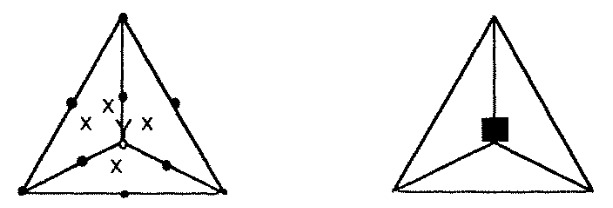
\includegraphics[width=6cm]{images/pair_cr/cr}\\
{\captionfont Taken from \textcite{begt92} (1992).}
\end{center}

The 3D version of this element is presented in \textcite{begt92} (1992). 
In their Table III we find the following node coordinates and basis functions:
\[
\begin{array}{lll}
\text{\# node} & \text{coordinates} & \text{basis function} \\
1  & (0,0,0) & \bN_1(r,s,t)=(1-r-s-t) -\frac12 (\bN_5+\bN_7+\bN_8)-\frac13(\bN_{11}+\bN_{12}+\bN_{13})-\bN_{15}/4 \\ 
2  & (1,0,0) & \bN_2(r,s,t)=r-\frac12(\bN_5+\bN_6+\bN_9)    -\frac13(\bN_{11}+\bN_{12}+\bN_{14}) -\bN_{15}/4 \\
3  & (0,1,0) & \bN_3(r,s,t)=s-\frac12(\bN_6+\bN_7+\bN_{10}) -\frac13(\bN_{11}+\bN_{13}+\bN_{14}) -\bN_{15}/4 \\
4  & (0,0,1) & \bN_4(r,s,t)=t-\frac12(\bN_8+\bN_9+\bN_{10}) -\frac13(\bN_{12}+\bN_{13}+\bN_{14}) -\bN_{15}/4 \\
5  & (\frac12,0,0)             &  \bN_5(r,s,t)=4(1-r-s-t)r-\frac49(\bN_{11}+\bN_{12})-\bN_{15}/4  \\
6  & (\frac12,\frac12,0)       &  \bN_6(r,s,t)=4rs-\frac49(\bN_{11}+\bN_{14})-\bN_{15}/4  \\
7  & (0,\frac12,0)             &  \bN_7(r,s,t)=4(1-r-s-t)s-\frac49(\bN_{11}+\bN_{13})-\bN_{15}/4  \\
8  & (0,0,\frac12)             &  \bN_8(r,s,t)=4(1-r-s-t)t-\frac49(\bN_{12}+\bN_{13})-\bN_{15}/4  \\
9  & (\frac12,0,\frac12)       &  \bN_9(r,s,t)=4rt-\frac49(\bN_{12}+\bN_{14})-\bN_{15}/4  \\
10 & (0,\frac12,\frac12)       &  \bN_{10}(r,s,t)= 4st-\frac49(\bN_{13}+\bN_{14})-\bN_{15}/4 \\
11 & (\frac13,\frac13,0)       &  \bN_{11}(r,s,t)= 27(1-r-s-t)rs-\frac{108}{256}\bN_{15} \\
12 & (\frac13,0,\frac13)       &  \bN_{12}(r,s,t)= 27(1-r-s-t)rt-\frac{108}{256}\bN_{15} \\
13 & (0,\frac13,\frac13)       &  \bN_{13}(r,s,t)= 27(1-r-s-t)st-\frac{108}{256}\bN_{15} \\
14 & (\frac13,\frac13,\frac13) &  \bN_{14}(r,s,t)= 27rst-\frac{108}{256}\bN_{15} \\
15 & (\frac14,\frac14,\frac14) &  \bN_{15}(r,s,t)= 256(1-r-s-t)rst \\
\end{array}
\]

We have
\begin{eqnarray}
\bN_1+\bN_2+\bN_3+\bN_4 
&=& (1-r-s-t) -\frac12 (\bN_5+\bN_7+\bN_8)-\frac13(\bN_{11}+\bN_{12}+\bN_{13})-\bN_{15}/4 \nn\\
&+& r-\frac12(\bN_5+\bN_6+\bN_9)    -\frac13(\bN_{11}+\bN_{12}+\bN_{14}) -\bN_{15}/4 \\
&+& s-\frac12(\bN_6+\bN_7+\bN_{10}) -\frac13(\bN_{11}+\bN_{13}+\bN_{14}) -\bN_{15}/4 \\
&+& t-\frac12(\bN_8+\bN_9+\bN_{10}) -\frac13(\bN_{12}+\bN_{13}+\bN_{14}) -\bN_{15}/4 \\
&=& 1 -\frac12(1+1)\bN_5 -\frac12(1+1)\bN_6 -\frac12(1+1)\bN_7 -\frac12(1+1)\bN_8 -\frac12(1+1)\bN_9 -\frac12(1+1)\bN_{10}    \nn\\
&&  -\frac13(1+1+1)\bN_{11} -\frac13(1+1+1)\bN_{12} -\frac13(1+1+1)\bN_{13} -\frac13(1+1+1)\bN_{14} 
-\frac{1}{4}(1+1+1+1)\bN_{15} \nn\\
&=& 1 -\bN_5 -\bN_6 -\bN_7 -\bN_8 -\bN_{9} -\bN_{10}
      -\bN_{11} -\bN_{12} -\bN_{13} -\bN_{14} -\bN_{15} 
\end{eqnarray}
So in the end
\[
\sum_{i=1}^{15} \bN_i = (\bN_1+\bN_2+\bN_3+\bN_4)  + \sum_{i=5}^{15} \bN_i = 0
\]

\begin{center}
\url{https://defelement.com/elements/conforming-crouzeix-raviart.html}
\end{center}





%----------------------------------------------------------------------
\subsubsection{The ${ P}_2^+\times P_{1}$ pair \label{ss:p2pp1}}
\begin{flushright} {\tiny {\color{gray} \tt  pair\_p2pp1.tex}} \end{flushright}
%~~~~~~~~~~~~~~~~~~~~~~~~~~~~~~~~~~~~~~~~~~~~~~~~~~~~~~~~~~~~~~~~~~~~~~~~~~~~~~~~~~~~~~~~~~~~~~~~~~

This element pair is not to be mistaken for the Crouzeix-Raviart. Both share the same $P_2^+$ space
for the velocity but this element has a continuous linear pressure.  
It is mentioned in Table~3.13-1 of \textcite{grsa}: ``LBB stable. Second order. cubic bubble. good element''.
It is also mentioned in \textcite{sofo87} (1987).

Implemented in \stone~120.


%------------------------------------------------------------------
\subsubsection{The ${ P}_2\times (P_1+P_0)$ pair} \label{ss:p2p1p0}
\begin{flushright} {\tiny {\color{gray} \tt pair\_p2p1p0.tex}} \end{flushright}
%~~~~~~~~~~~~~~~~~~~~~~~~~~~~~~~~~~~~~~~~~~~~~~~~~~~~~~~~~~~~~~~~~~~~~~~~~~~~~~~~~~~~~~~~~~~~~~~~~~

This element pair is discussed in 5.3.3 of Elman, Silvester and Wathen: 
\begin{displayquote}
{\color{darkgray}
[Another] possibility is to construct a hybrid pressure approximation by 
combining the continuous linear pressure approximation with the 
discontinuous constant pressure approximation. The resulting mixed method 
is referred to as the $P_2-P_{-1*}$ 
approximation and enjoys the best of both worlds; it has locally 
incompressibility, and yet it does not have its accuracy compromised by
the lower order pressure [of $P_2\times P_0$]. 
Perhaps surprisingly, this element is also uniformly stable.
}
\end{displayquote}

\begin{center}
\includegraphics[width=7cm]{images/pair_p2p1p0/elsw}\\
{\captionfont Taken from \textcite{elsw}.}
\end{center}

In Gresho \& Sani table 3.13-1: 
``LBB stable yes. Better than P2P1, element mass balance.
more work than P2P1. 2 hydrostatic modes. Second order.'' 

\begin{center}
\includegraphics[width=4cm]{images/pair_p2p1p0/grsa2}
\includegraphics[width=12cm]{images/pair_p2p1p0/grsa1}\\
{\captionfont Taken from \textcite{grsa}. Unfortunately they do not 
provide a source for 
its origin, for the LBB-stability proof, or any source at all, actually.}
\end{center}

Looking at the figure above, it is clear that the $P_1$ space is to be understood 
as a continuous pressure space, with an additional constant bubble. 

For the continuous $P_1$ space, we have the following reference element
\begin{center}
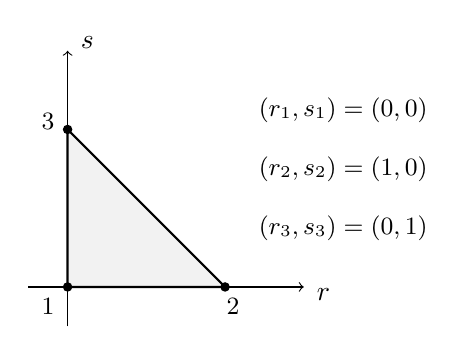
\begin{tikzpicture}
\draw[fill=gray!10,gray!10] (0.5,0.5)--(2.5,0.5)--(0.5,2.5)--cycle;
\draw[thick] (0.5,0.5)--(2.5,0.5)--(0.5,2.5)--cycle;
\draw [->] (0,0.5) -- (3.5,0.5);
\draw [->] (0.5,0) -- (0.5,3.5);
\node[] at (3.75,0.4) {$r$};
\node[] at (0.75,3.6) {$s$};
\draw[black,fill=black] (0.5,0.5)   circle (1.5pt);
\draw[black,fill=black] (2.5,0.5)   circle (1.5pt);
\draw[black,fill=black] (0.5,2.5)   circle (1.5pt);
\node[] at (0.25,0.25) {\small $1$};
\node[] at (2.6,0.25) {\small $2$};
\node[] at (0.25,2.6) {\small $3$};
\node[] at (4,2.75) {\small $(r_1,s_1)=(0,0)$};
\node[] at (4,2) {\small $(r_2,s_2)=(1,0)$};
\node[] at (4,1.25) {\small $(r_3,s_3)=(0,1)$};
\end{tikzpicture}
\end{center}
and the basis functions are simply
\begin{eqnarray}
\bN_1(r,s) &=& 1-r-s \\
\bN_2(r,s) &=& r \\
\bN_3(r,s) &=& s 
\end{eqnarray}
with the interpolation requirement $\bN_i(r_j,s_j)=\delta_{ij}$ fulfilled, 
as well as $\sum_i \bN_i=1$. 

Now, following the figure by Gresho and Sani, I build the reference element for the $P_1+P_0$ space:
\begin{center}
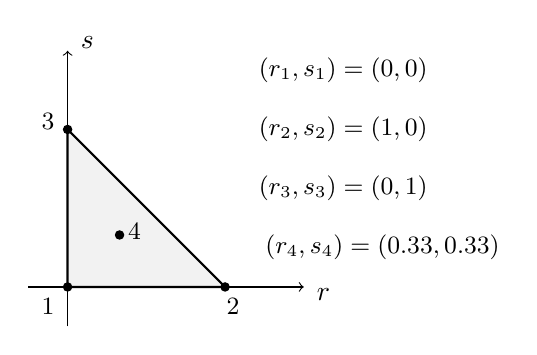
\begin{tikzpicture}
\draw[fill=gray!10,gray!10] (0.5,0.5)--(2.5,0.5)--(0.5,2.5)--cycle;
\draw[thick] (0.5,0.5)--(2.5,0.5)--(0.5,2.5)--cycle;
\draw [->] (0,0.5) -- (3.5,0.5);
\draw [->] (0.5,0) -- (0.5,3.5);
\node[] at (3.75,0.4) {$r$};
\node[] at (0.75,3.6) {$s$};
\draw[black,fill=black] (0.5,0.5)   circle (1.5pt);
\draw[black,fill=black] (2.5,0.5)   circle (1.5pt);
\draw[black,fill=black] (0.5,2.5)   circle (1.5pt);
\draw[black,fill=black] (1.16,1.16) circle (1.5pt);
\node[] at (0.25,0.25) {\small $1$};
\node[] at (2.6,0.25) {\small $2$};
\node[] at (0.25,2.6) {\small $3$};
\node[] at (1.35,1.2) {\small $4$};
\node[] at (4,3.25) {\small $(r_1,s_1)=(0,0)$};
\node[] at (4,2.5)    {\small $(r_2,s_2)=(1,0)$};
\node[] at (4,1.75) {\small $(r_3,s_3)=(0,1)$};
\node[] at (4.5,1) {\small $(r_4,s_4)=(0.33,0.33)$};
\end{tikzpicture}
\end{center}

$P_1+P_0$ means that the pressure inside the element is given by
\[
p^h(r,s) = a \bN_1(r,s)+ b\bN_2(r,s) + c\bN_3(r,s) + d\bN_4(r,s) 
\]
Note that it is then impossible to find $a,b,c,d$ such that the interpolation 
requirement $\bN_i(r_j,s_j)=\delta_{ij}$ is fulfilled.
In other words, the element is not interpolatory, i.e., there is no $\delta_{ij}$ property.% W.B. email

With regards to the 'element mass balance', W.B. states : 
\begin{displayquote}
{\color{darkgray}
the mass conservation requires that the function that is constant 1 
on one cell and zero on all other cells is part of the function space. 
That is indeed true -- it's the $\bN_4$ function. Indeed, that's the purpose of 
the enrichment with the $P_0$ part. It is not necessary that {\it all} shape functions are discontinuous.
}
\end{displayquote}




\textcite{bocg12} (2012) state: 
\begin{displayquote}
{\color{darkgray}
[...] the pressure space $Q_h$ is defined as the sum of two finite 
element spaces, namely $P_k+P_0$ ($k \ge d- 1$) [...] for the enhanced 
Hood–Taylor [...]. However, it can be easily observed that the sum is not direct, 
since globally constant functions can be represented exactly by means of piecewise 
$P_0$ or continuous $P_k$ ($k \ge 1$) elements.
Concerning the implementation of the method, we avoid the computation of the basis
functions of such a finite element by testing the discrete problem (2.3) 
with the basis 
functions of the two subspaces separately. By the above discussion it 
turns out that the resulting
matrix is rank-deficient, with kernel of dimension 1.
}
\end{displayquote}

The element pair is also discussed in \textcite{chen14} (2014).



%------------------------------------------------------------------
\subsubsection{The ${ Q}_2\times (Q_1+Q_0)$ pair} \label{ss:q2q1q0}
\begin{flushright} {\tiny {\color{gray} \tt  pair\_q2q1q0.tex}} \end{flushright}
%~~~~~~~~~~~~~~~~~~~~~~~~~~~~~~~~~~~~~~~~~~~~~~~~~~~~~~~~~~~~~~~~~~~~~~~~~~~~~~~~~~~~~~~~~~~~~~~~~~

It is a rather peculiar element pair (triplet?). The velocity space is the standard $Q_2$ space
but the pressure space is the sum of two spaces, i.e. $Q_1$ {\it and} $Q_0$.
Please see Section~\ref{ss:p2p1p0} on the ${\bm P}_2\times (P_1+P_0)$ element.

\begin{center}
\includegraphics[width=9cm]{images/pair_q2q1q0}\\
{\captionfont Taken from \textcite{grsa}'s book.}
\end{center}

It is implemented in \stone~120.


%------------------------------------------------------------------
\subsubsection{The ${ P}_3\times P_2$ pair} \label{ss:p3p2}
\index{general}{$P_3\times P_2 element$}
\begin{flushright} {\tiny {\color{gray} \tt pair\_p3p2.tex}} \end{flushright}
%~~~~~~~~~~~~~~~~~~~~~~~~~~~~~~~~~~~~~~~~~~~~~~~~~~~~~~~~~~~~~~~~~~~~~~~~~~~~~~~~~~~~~~~~~~~~~~~~~~

${\bm P}_3\times P_2$ mentioned in \textcite{sten90}.
The $P_3$ basis functions are presented in Section~\ref{basis:p3} and the $P_2$ basis
functions in Section~\ref{basis:p2}.
See \stone~120.


%------------------------------------------------------------------
\subsubsection{The Raviart-Thomas family} \label{ss:raviart_thomas}
\begin{flushright} {\tiny {\color{gray} \tt pair\_raviart\_thomas.tex}} \end{flushright}
%~~~~~~~~~~~~~~~~~~~~~~~~~~~~~~~~~~~~~~~~~~~~~~~~~~~~~~~~~~~~~~~~~~~~~~~~~~~~~~~~~~~~~~~~~~~~~~~~~~

- Raviart Thomas 0 RT0 \cite{rath77} ? mentioned/defined/drawn in 4.2.2 of 
Kanschat book. Also exist for quads see 4.2.37 
\textcite{hald03}: ``$P_1^\perp \times P_0$ symbol denotes an element with 
normal velocity nodes in the middle of each edge of the
triangulation [...]. This element, also called low order Raviart–Thomas element 
(Raviart and Thomas, 1977), is based on flux conservation on elements edges and 
the resulting scheme is very close to a finite volume scheme.''

Mentioned in \textcite{john16}, appendix B.3, example B.45: ``the normal component of v 
on each face is a constant. The normal component of functions from RT0 is
continuous across faces of the mesh cells.''

Check \textcite{brfo}

Mentioned in \textcite{chen93a} (1993).

\url{https://defelement.com/elements/raviart-thomas.html}


\url{
https://en.wikipedia.org/wiki/Raviart-Thomas_basis_functions
}

\url{
https://people.tamu.edu/~guermond//M661_FALL_2015/chap7.pdf
}

\url{
https://scicomp.stackexchange.com/questions/20245/raviart-thomas-elements-on-reference-square
}





%------------------------------------------------------------------
\subsubsection{The Bernaudi-Raugel pair} \label{ss:bernaudi_raugel}
\begin{flushright} {\tiny {\color{gray} pair\_bernaudi\_raugel.tex}} \end{flushright}
%~~~~~~~~~~~~~~~~~~~~~~~~~~~~~~~~~~~~~~~~~~~~~~~~~~~~~~~~~~~~~~~~~~~~~~~~~~~~~~~~~~~~~~~~~~~~~~~~~~

In \textcite{cakp15} (2015) we find: ``The BR-FEM after Bernardi and Raugel \cite{bera85} 
is a modification of the $P_2\times P_0$ FEM. It is sometimes also called reduced $P_2\times P_0$ FEM''.
They also state that this element also exists in 3D.

\begin{center}
\includegraphics[width=5cm]{images/pair_bernardi_raugel/cakp15}
\end{center}

It is also mentioned in \textcite{bobf13} although it seems it is there called the SMALL element (p474).

In Lederer: "Consider the case d = 2. [...] we only need to control 
the normal velocity at the edge, i.e. adding the
edge bubble for both components of the velocity seems to be sub optimal (with respect to
computational costs and the expected approximation properties). The idea now is to only
add the normal edge bubble."

According to \textcite{jolm17} (2017) (example 6.3), `` the velocity space in the Bernardi-Raugel
element consists of $P_1$ functions which are enriched with edge bubble functions''.
The authors also speak of 'reconstructing the test functions' and state: 
``the results of the method with reconstruction are generally more accurate.
In summary, the use of an appropriately reconstructed test function in the Bernardi–
Raugel pair of spaces led to a clear improvement of the accuracy of the computed
results compared with the standard method.''




%------------------------------------------------------------------
\subsubsection{The Scott-Vogelius pair} \label{ss:scott_vogelius}
\index{general}{Scott-Vogelius pair}
\begin{flushright} {\tiny {\color{gray} \tt pair\_scott\_vogelius.tex}} \end{flushright}
%~~~~~~~~~~~~~~~~~~~~~~~~~~~~~~~~~~~~~~~~~~~~~~~~~~~~~~~~~~~~~~~~~~~~~~~~~~~~~~~~~~~~~~~~~~~~~~~~~~

It originates in \fullcite{scvo85} (1985). 

 
In Remark 9 (p.29) of \textcite{aubb17} (2017) we find: 
\begin{displayquote}
{\color{darkgray}
We also remark that the discontinuous
pressure version of the Hood–Taylor element typically
results in an unstable method. However, stability can be
recovered by imposing certain restrictions on the mesh for
$k \ge 3$ (see \cite{voge83}; \cite{scvo85}), or
by taking advantage of suitable stabilization procedures for
$k\ge 1$ (see Mansfield, 1982; Boffi, 1995).
}
\end{displayquote}

In \textcite{fams21} (2021) we find:
\begin{displayquote}
{\color{darkgray}
The Scott-Vogelius element is given by choosing continuous piecewise 
polynomials of degree $k$ for the velocity and discontinuous piecewise 
polynomials of degree $k-1$ for the pressure. While this clearly
implies that $\nabla\cdot V_h \in Q_h$, inf-sup stability of the 
Scott–Vogelius element is more delicate, and is a topic of ongoing research. 
In two dimensions, Scott \& Vogelius proved \cite{scvo85} that the element is inf-sup
stable for $k\ge 4$ if the mesh does not have nearly singular vertices. 
In three dimensions, it was proven more recently in \cite{zhan11b} 
that the element is stable for $k\ge 6$ on uniform meshes. The stability on general
tetrahedral meshes continues to be an open question.

On barycentrically refined meshes, however, the pair is known to 
be stable for polynomial order
$k = d$, see [48, Section 4.6] for the 2D case and 
\cite{zhan05} for the 3D case. If one is willing to 
consider the more complicated Powell–Sabin split, the order 
can be reduced further to $k=d-1$ \cite{zhan08,zhan11a}. The two
refinement patterns are shown for the two dimensional case 
in Figure 1 [see below]. In this work we will consider
the case of $k \ge d$ on barycentrically refined meshes, but 
the arguments apply mutatis mutandis to the Powell–Sabin split.
}
\end{displayquote}

\begin{center}
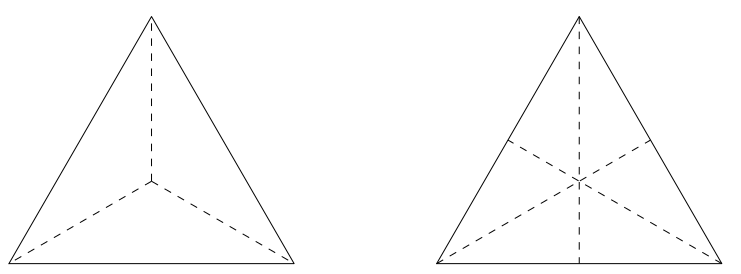
\includegraphics[width=9cm]{images/pair_scott_vogelius/scottvogelius_split}\\
{\captionfont 
Barycentrically refined triangle (also known as Alfeld split) on the left,
and Powell–Sabin split on the right.\\ Taken from \textcite{fams21} (2021).}
\end{center}

\index{general}{Powell-Sabin}

\textcite{cael11} (2011) state:
\begin{displayquote}
{\color{darkgray}
The SV element pair is not yet very well known,
and so we now give a brief description of it. In essence, the SV pair is the same as
the Taylor-Hood pair except that the pressure space is discontinuous and either
(i) for $k \ge d$, the mesh is a barycenter refinement of a regular mesh, or
(ii) for $k = 2, d = 3$, the mesh is formed from a barycenter refined mesh by
connecting the barycenter nodes (i.e., a Powell–Sabin tetrahedralization).
In short, polynomials of degree $k$ and $k-1$ are used to approximate the velocity
and pressure spaces, respectively, and the mesh ${\cal T}_h$ that is used must be derived from
a regular triangulation (tetrahedralization) of $\Omega$, where each element is refined as
stated above. With these mesh constructions, it was proved by Zhang in [42, 44] that
the SV elements are LBB stable, and, consequently, also have optimal approximation
properties. It is well known that the TH pair is LBB stable and admits optimal
approximation properties for these cases as well [9]. We will restrict our definition of
SV elements to these cases where they are LBB stable.
}
\end{displayquote}

On page 112 of \textcite{john16} we read:
\begin{displayquote}
{\color{darkgray}
The Scott–Vogelius finite element considers still $P_k/P^{disc}_{k-1}$, $k \ge d$, 
but on special meshes, which allow to show the satisfaction of the 
discrete inf-sup condition.
[...]
This pair of finite element spaces $P_k/P^{disc}_{k-1}$
are weakly divergence-free, which is a desirable property.
[...]
The fulfillment of the discrete inf-sup condition 
was proved already in \textcite{scvo85} (1985) in the two-dimensional 
case for $k\ge 4$ if there is no so-called singular vertex in the mesh.
An internal vertex is said to be singular if edges which meet at the vertex fall onto
two straight lines.

The basic idea to overcome this problem consists in using meshes 
without singular vertices. To this end, so-called barycentric-refined 
grids are constructed. Starting from any admissible triangular mesh, 
new edges are introduced by connecting all
vertices of a mesh cell with the barycenter of this mesh cell. 
This step creates smaller triangles.
On barycentric-refined meshes, the $P_k/P^{disc}_{k-1}$, $k=2,3$ 
pair of finite element spaces was shown to satisfy the discrete inf-sup
condition in Qin's phd thesis (1994). [...]

The use of the $P_2/P^{disc}_{1}$ pair of finite element spaces 
on barycentric-refined meshes can be found occasionally in the literature,
in particular to demonstrate the advantages of using pairs of finite element 
spaces which provide weakly divergence-free velocity solutions, 
e.g. see \textcite{john15} and refs therein.

}
\end{displayquote}


\begin{center}
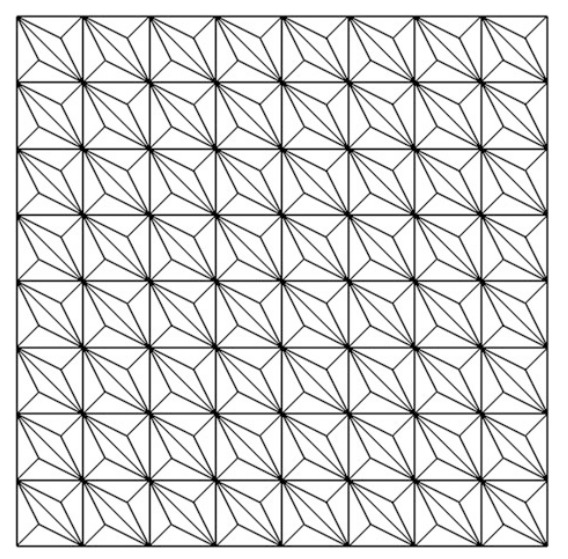
\includegraphics[width=6cm]{images/pair_scott_vogelius/john16}\\
{\captionfont Barycentric-refined simplicial grid on the unit square}
\end{center}

I hereafter present my own internal numbering for the mesh above (used in \stone~120 for example).
The quadrilateral has been cut once along a diagonal, and then an Alfeld split is used, thereby 
dividing the square in 6 triangles:

\begin{flushright} {\tiny {\color{gray} (tikz\_sv.tex)}} \end{flushright}
%~~~~~~~~~~~~~~~~~~~~~~~~~~~~~~~~~~~~~~~~~~~~~~~~~~~~~~~~~~~~~~~~~~~~~~~~~~~~~~~~~~~~~~~~~~~~~~~~~~


\begin{center} 
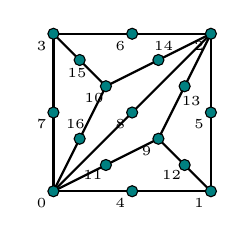
\begin{tikzpicture} 

%\draw[fill=gray!23,gray!23](0,0) rectangle (2.5,2.5);
%\draw[step=0.5cm,gray,very thin] (0,0) grid (2.5,2.5); %background grid

%ielx=1,iely=1,low
\draw[thick] (0,0)--(1.33333,0.66667);
\draw[thick] (2,0)--(1.33333,0.66667);
\draw[thick] (2,2)--(1.33333,0.66667);
%ielx=1,iely=1,high
\draw[thick] (0,0)--(0.666667,1.3333);
\draw[thick] (0,2)--(0.666667,1.3333);
\draw[thick] (2,2)--(0.666667,1.3333);

\draw[thick] (0,0) -- (2,0) -- (2,2) -- (0,2) -- cycle; 
\draw[thick] (0,0) -- (2,2) ; %diag


%\draw[thick] (6,0) -- (4,2) -- (6,4) ; 
\draw[black,fill=teal] ( 0.000000 , 0.000000)     circle (2pt); 
\node[] at ( -0.150000, -0.150000 ) {\tiny 0 }; 
\draw[black,fill=teal] ( 2.000000 , 0.000000)     circle (2pt); 
\node[] at ( 1.850000, -0.150000 ) {\tiny 1 }; 
\draw[black,fill=teal] ( 2.000000 , 2.000000)     circle (2pt); 
\node[] at ( 1.850000, 1.850000 ) {\tiny 2 }; 
\draw[black,fill=teal] ( 0.000000 , 2.000000)     circle (2pt); 
\node[] at ( -0.150000, 1.850000 ) {\tiny 3 }; 
\draw[black,fill=teal] ( 1.000000 , 0.000000)     circle (2pt); 
\node[] at ( 0.850000, -0.150000 ) {\tiny 4 }; 
\draw[black,fill=teal] ( 2.000000 , 1.000000)     circle (2pt); 
\node[] at ( 1.850000, 0.850000 ) {\tiny 5 }; 
\draw[black,fill=teal] ( 1.000000 , 2.000000)     circle (2pt); 
\node[] at ( 0.850000, 1.850000 ) {\tiny 6 }; 
\draw[black,fill=teal] ( 0.000000 , 1.000000)     circle (2pt); 
\node[] at ( -0.150000, 0.850000 ) {\tiny 7 }; 
\draw[black,fill=teal] ( 1.000000 , 1.000000)     circle (2pt); 
\node[] at ( 0.850000, 0.850000 ) {\tiny 8 }; 
\draw[black,fill=teal] ( 1.333333 , 0.666667)     circle (2pt); 
\node[] at ( 1.183333, 0.516667 ) {\tiny 9 }; 
\draw[black,fill=teal] ( 0.666667 , 1.333333)     circle (2pt); 
\node[] at ( 0.516667, 1.183333 ) {\tiny 10 }; 
\draw[black,fill=teal] ( 0.666667 , 0.3333)     circle (2pt); 
\node[] at ( 0.5, 0.2 ) {\tiny 11 }; 
\draw[black,fill=teal] ( 1.6667 , 0.3333)     circle (2pt); 
\node[] at ( 1.5, 0.2 ) {\tiny 12 }; 
\draw[black,fill=teal] ( 1.6667 , 1.3333)     circle (2pt); 
\node[] at ( 1.75, 1.15 ) {\tiny 13 }; 
\draw[black,fill=teal] ( 0.3333,0.666667)     circle (2pt); 
\node[] at ( 1.4,1.85 ) {\tiny 14}; 
\draw[black,fill=teal] ( 0.3333, 1.6667)     circle (2pt); 
\node[] at ( 0.3,1.5 ) {\tiny 15 }; 
\draw[black,fill=teal] ( 1.3333, 1.6667)     circle (2pt); 
\node[] at ( 0.28,0.85 ) {\tiny 16 }; 


\end{tikzpicture} 
%\end{center} 


%\begin{center} 
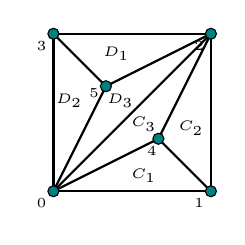
\begin{tikzpicture} 

%\draw[fill=gray!23,gray!23](0,0) rectangle (2.5,2.5);
%\draw[step=0.5cm,gray,very thin] (0,0) grid (2.5,2.5); %background grid

%ielx=1,iely=1,low
\draw[thick] (0,0)--(1.33333,0.66667);
\draw[thick] (2,0)--(1.33333,0.66667);
\draw[thick] (2,2)--(1.33333,0.66667);
%ielx=1,iely=1,high
\draw[thick] (0,0)--(0.666667,1.3333);
\draw[thick] (0,2)--(0.666667,1.3333);
\draw[thick] (2,2)--(0.666667,1.3333);

\draw[thick] (0,0) -- (2,0) -- (2,2) -- (0,2) -- cycle; 
\draw[thick] (0,0) -- (2,2) ; %diag

%\draw[thick] (6,0) -- (4,2) -- (6,4) ; 
\draw[black,fill=teal] ( 0.000000 , 0.000000)     circle (2pt); 
\node[] at ( -0.150000, -0.150000 ) {\tiny 0 }; 
\draw[black,fill=teal] ( 2.000000 , 0.000000)     circle (2pt); 
\node[] at ( 1.850000, -0.150000 ) {\tiny 1 }; 
\draw[black,fill=teal] ( 0.000000 , 2.000000)     circle (2pt); 
\node[] at ( -0.150000, 1.850000 ) {\tiny 3 }; 
\draw[black,fill=teal] ( 2.000000 , 2.000000)     circle (2pt); 
\node[] at ( 1.850000, 1.850000 ) {\tiny 2 }; 
\draw[black,fill=teal] ( 1.333333 , 0.666667)     circle (2pt); 
\node[] at ( 1.25, 0.516667 ) {\tiny 4 }; 
\draw[black,fill=teal] ( 0.666667 , 1.333333)     circle (2pt); 
\node[] at ( 0.516667, 1.25 ) {\tiny 5 }; 

\node[] at ( 1.15,0.2 ) {\tiny $C_1$ }; 
\node[] at ( 1.75,0.8 ) {\tiny $C_2$ }; 
\node[] at ( 1.15,0.85 ) {\tiny $C_3$ }; 

\node[] at ( 0.8,1.75 ) {\tiny $D_1$ }; 
\node[] at ( 0.2,1.15 ) {\tiny $D_2$ }; 
\node[] at ( 0.85,1.15 ) {\tiny $D_3$ }; 

\end{tikzpicture} 
\end{center} 



See also \textcite{jolm17} (2017) in which the $P_2\times P_1$, Scott-Vogelius ($P_2\times P_{-1}$), 
Bernardi-Raugel, and $P_2^+\times P_{-1}$ elements 
are compared for a thermo-mechanically driven convection problem in a triangle (see \stone~51, 
although I use the $P_1^+\times P_1$ element in this stone).


\begin{center}
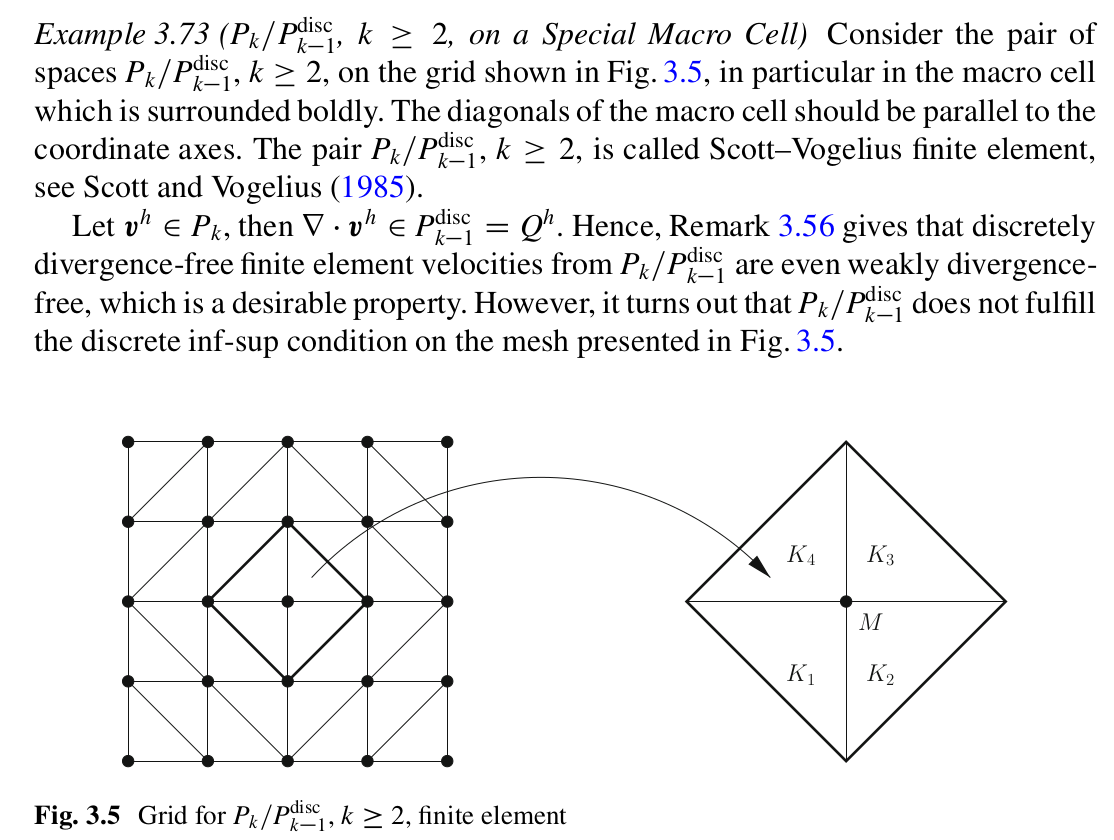
\includegraphics[width=10cm]{images/pair_scott_vogelius/john_scott_vogelius}\\
\captionfont{Taken from John \cite[p70]{john16}.} 
\end{center}


In \textcite{befh21} (2021) this element is used in its 
$(P_3)^2-P_2^{\text{disc}}$ form.

Note that some have proposed to use an incenter-based refinement instead of
a barycenter refinement since it lead to less pronounced aspect ratios\footnote{
The Scott-Vogelius Method for Stokes Problem on Anisotropic Meshes, K Kean, M Neilan, M Schneier,
\url{https://doi.org/10.48550/arXiv.2109.14780}}.
In geometry, the incenter of a triangle is a triangle center, a point defined for 
any triangle in a way that is independent of the triangle's placement or scale. 
The incenter may be equivalently defined as the point where the internal angle bisectors 
of the triangle cross or as the point equidistant from the triangle's sides.

Given the coordinates of the three vertices of a triangle ABC,
the coordinates of the incenter O are
\[
x_O=\frac{ax_A+bx_B+cx_C}{a+b+c}
\qquad
y_O=\frac{ay_A+by_B+cy_C}{a+b+c}
\] 
where $a$, $b$ and $c$ are the side lengths opposite vertex A, B and C.

 
Note that \textcite{zhan24} (2024) proposes a solution to the unstable issue: 
\begin{displayquote}
{\color{darkgray}
We show that the discrete velocity solution converges at
the optimal order when solving the steady state Stokes
equations by the ${\bm P}_k\times P_{-(k-1)}$ mixed finite element method for
$k \ge 4$ on 2D triangular grids or $k \ge 6$ on tetrahedral grids,
even in the case the inf-sup condition fails. By a simple
$L_2$-projection of the discrete $P_{k-1}$ pressure to the space of
continuous $P_{k-1}$ polynomials, we show this post-processed
pressure solution also converges at the optimal order. Both
2D and 3D numerical tests are presented, verifying the
theory.
}
\end{displayquote}

Rather interestingly, we find in \textcite{tesk12} (2012) a penalty-approach:
\begin{displayquote}
{\color{darkgray}
Other solutions to deal with the LBB condition include the Uzawa iteration method and penalty
methods. A combination of these two approaches results in the iterated penalty method presented in
Scott and Vogelius (1985). Let $r\in\R$ and $\rho\in\R^+$ be prescribed parameters. 
We wish to find $u^n\in V_h$ such that 
\[
a(u^n,v) + r(\nabla\cdot u^n,\nabla\cdot v) = (f,v) - (\nabla \cdot v, \nabla\cdot w^n)
\qquad \forall \; v\in V_h,
\]
where $w^{n+1}=w^n+\rho u^n$.
The pressure may be recovered from the auxiliary field $w$ via $p=\nabla\cdot w -C$, 
where $C$ is an arbitrary constant (since the pressure field is only determined up 
to an arbitrary constant). When computing the error in $p$, we subtract the average 
of $\nabla\cdot w$ to account for $C$. The algorithm initially assumes
$w^0=0$, and then solves [the equation above] and updates $w$. 
The process is repeated until $\| u^{n+1}-u^n\|<\epsilon$, 
where $\epsilon$ is a prescribed tolerance. This method involves only one function space, but
it requires a higher-order continuous element $(q\ge 4)$ and it solves the divergence-free criterion
exactly. The iteration count and accuracy are dependent upon the penalty parameters $\rho$ and $r$. 
The implementation of this formulation is presented in [the following figure]:
\begin{center}
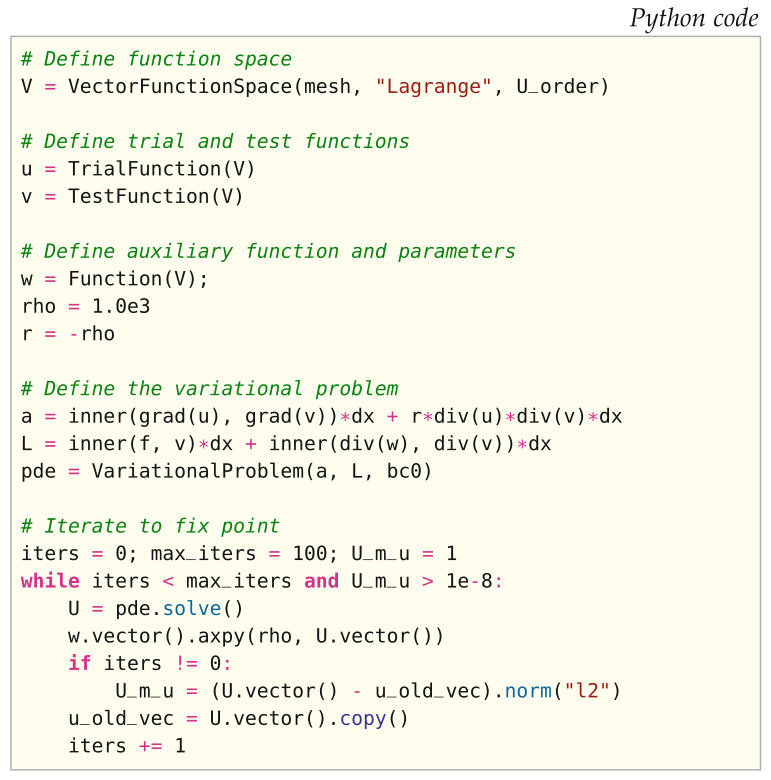
\includegraphics[width=6cm]{images/pair_scott_vogelius/tesk12}
\end{center}

}
\end{displayquote}



\begin{center}
\url{https://defelement.com/elements/scott-vogelius.html}
\end{center}




%------------------------------------------------------------------
\subsubsection{The BDM (Brezzi-Douglas-Marini) pair} \label{ss:bdm}
\index{general}{BDM element}
\index{general}{BDM element}
\begin{flushright} {\tiny {\color{gray} \tt  pair\_bdm.tex}} \end{flushright}
%~~~~~~~~~~~~~~~~~~~~~~~~~~~~~~~~~~~~~~~~~~~~~~~~~~~~~~~~~~~~~~~~~~~~~~~~~~~~~~~~~~~~~~~~~~~~~~~~~~

This element is mentioned in Kanschat book \cite{kanschat}, section 4.2.14. 
It also exists for quads see section 4.2.39 in the same book.
It is mentioned in \textcite{chen93a} (1993), also check the book by \textcite{brfo}.
It is well described in \textcite{kanschat17}.
There is an entire chapter (14) of \textcite{ergu21_72} dedicated to H(div) and 
section 14.5.1 to BDM elements. 
Check section 4.1.1 of \cite{aubb17} for triangles and quads.

\begin{center}
\url{https://defelement.com/elements/brezzi-douglas-marini.html}
\end{center}

\begin{itemize}
%++++++++++++++++++++++++++++++++++++++++++++++
\item In \textcite{lomw12} we read:

The Brezzi-Douglas-Marini element was introduced by Brezzi, Douglas and Marini in two dimensions 
(for triangles) in \textcite{brdm85} (1985). The element can be viewed as an alternative to the
Raviart-Thomas element using a complete polynomial space. It was later extended to three 
dimensions (tetrahedra, prisms and cubes) in \textcite{nede86} (1986) 
and \textcite{brdd87} (1987). The definition given
here is based on that of \textcite{nede86} (1986).

The Brezzi-Douglas-Marini element was introduced for mixed formulations of second-order elliptic 
equations. However, it is also useful for weakly symmetric discretizations of the elastic stress
tensor; see Farhloul and Fortin (1997); Arnold et al. (2007).

\begin{center}
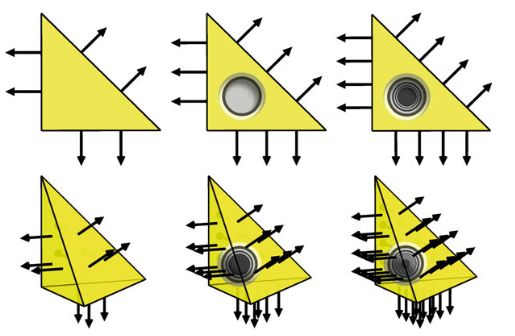
\includegraphics[width=8cm]{images/pair_bdm/bdm_lomw12}\\
{\captionfont Taken from \cite{lomw12}. }
\end{center}

The dimension of $BDM_q$ is $(q+1)(q+2)$ for a triangle and $\frac12(q+1)(q+2)(q+3)$
for a tetrahedron.

Check book for definition.

A slight modification of the Brezzi-Douglas-Marini element constrains the element space ${\cal V}$ by
only allowing normal components on the boundary of polynomial degree $q-1$ (rather than the full
polynomial degree $q$). Such an element was suggested on rectangles by \textcite{brdf87} (1987), and the
triangular analogue was given in \textcite{brfo}. In similar spirit, elements with differing
degrees on the boundary suitable for varying the polynomial degree between triangles were derived
in \textcite{brdm85b} (1985).

%++++++++++++++++++++++++++++++++++++++++++++++
\item On the defelement website\footnote{\url{https://defelement.org/elements/brezzi-douglas-marini.html}}
we find a lot of information. Note that the mapping is set to 'contravariant Piola'. 
\todo[inline]{I still need to understand and write about this!}
It belongs to the categories 'Vector-valued elements', and 'H(div) conforming elements'

\begin{center}
% -------------------------------------------------------
% This plot is from DefElement (https://defelement.org)
% and is available under a Creative Commons Attribution
% 4.0 International (CC BY 4.0) license:
% https://creativecommons.org/licenses/by/4.0/
% -------------------------------------------------------
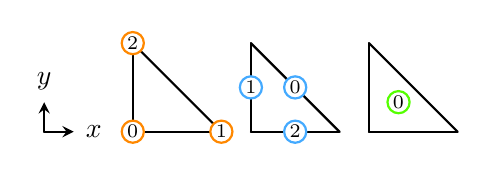
\begin{tikzpicture}[x=1cm,y=1cm]
\definecolor{customcolor0}{HTML}{000000}
\definecolor{customcolor1}{HTML}{44AAFF}
\definecolor{customcolor2}{HTML}{AAAAAA}
\definecolor{customcolor3}{HTML}{DD2299}
\definecolor{customcolor4}{HTML}{FFFFFF}
\definecolor{customcolor5}{HTML}{FF8800}
\definecolor{customcolor6}{HTML}{55FF00}
\draw[-stealth,customcolor0,line width=0.8pt,line cap=round] (25.0,25.0) -- (25.375,25.0);
\draw[-stealth,customcolor0,line width=0.8pt,line cap=round] (25.0,25.0) -- (25.0,25.375);
\node[customcolor0,anchor=west] at (25.405,25.0) {$x$};\node[customcolor0,anchor=south] at (25.0,25.405) {$y$};\draw[customcolor0,line width=0.8pt,line cap=round] (27.25,25.0) -- (26.125,26.125);
\draw[customcolor0,line width=0.8pt,line cap=round] (26.125,25.0) -- (26.125,26.125);
\draw[customcolor0,line width=0.8pt,line cap=round] (26.125,25.0) -- (27.25,25.0);
\draw[customcolor5,line width=0.8pt,fill=customcolor4] (26.125,25.0) circle (4.0pt);
\node[customcolor0,anchor=center] at (26.125,25.0) {\scriptsize 0};\draw[customcolor5,line width=0.8pt,fill=customcolor4] (27.25,25.0) circle (4.0pt);
\node[customcolor0,anchor=center] at (27.25,25.0) {\scriptsize 1};\draw[customcolor5,line width=0.8pt,fill=customcolor4] (26.125,26.125) circle (4.0pt);
\node[customcolor0,anchor=center] at (26.125,26.125) {\scriptsize 2};\draw[customcolor0,line width=0.8pt,line cap=round] (28.75,25.0) -- (27.625,26.125);
\draw[customcolor1,line width=0.8pt,fill=customcolor4] (28.1875,25.5625) circle (4.0pt);
\node[customcolor0,anchor=center] at (28.1875,25.5625) {\scriptsize 0};\draw[customcolor0,line width=0.8pt,line cap=round] (27.625,25.0) -- (27.625,26.125);
\draw[customcolor1,line width=0.8pt,fill=customcolor4] (27.625,25.5625) circle (4.0pt);
\node[customcolor0,anchor=center] at (27.625,25.5625) {\scriptsize 1};\draw[customcolor0,line width=0.8pt,line cap=round] (27.625,25.0) -- (28.75,25.0);
\draw[customcolor1,line width=0.8pt,fill=customcolor4] (28.1875,25.0) circle (4.0pt);
\node[customcolor0,anchor=center] at (28.1875,25.0) {\scriptsize 2};\draw[customcolor6,line width=0.8pt,fill=customcolor4] (29.5,25.375) circle (4.0pt);
\node[customcolor0,anchor=center] at (29.5,25.375) {\scriptsize 0};\draw[customcolor0,line width=0.8pt,line cap=round] (30.25,25.0) -- (29.125,26.125);
\draw[customcolor0,line width=0.8pt,line cap=round] (29.125,25.0) -- (29.125,26.125);
\draw[customcolor0,line width=0.8pt,line cap=round] (29.125,25.0) -- (30.25,25.0);
\end{tikzpicture}
\\
{\captionfont Taken from DefElement \url{https://defelement.org/img/ref-triangle.html}. I have altered 
the font size. Orange: nodes; Blue: edges.}
\end{center}


I reproduce below the figures and basis functions pertaining to the Degree 1 triangle, 
but the site also shows Degree 2 triangle, Degree 1 \& 2 tetrahedron, and so-called 
Lagrange variants.

\begin{center}
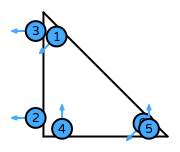
\includegraphics[width=3cm]{images/pair_bdm/element-Brezzi-Douglas-Marini-variant-equispaced-triangle-1-dofs}
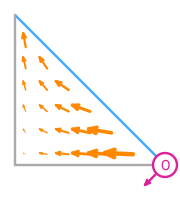
\includegraphics[width=3cm]{images/pair_bdm/element-Brezzi-Douglas-Marini-variant-equispaced-triangle-1-0}
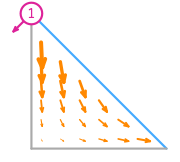
\includegraphics[width=3cm]{images/pair_bdm/element-Brezzi-Douglas-Marini-variant-equispaced-triangle-1-1}
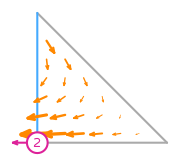
\includegraphics[width=3cm]{images/pair_bdm/element-Brezzi-Douglas-Marini-variant-equispaced-triangle-1-2}\\
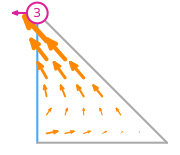
\includegraphics[width=3cm]{images/pair_bdm/element-Brezzi-Douglas-Marini-variant-equispaced-triangle-1-3}
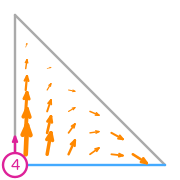
\includegraphics[width=3cm]{images/pair_bdm/element-Brezzi-Douglas-Marini-variant-equispaced-triangle-1-4}
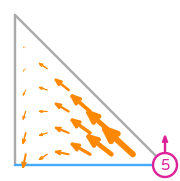
\includegraphics[width=3cm]{images/pair_bdm/element-Brezzi-Douglas-Marini-variant-equispaced-triangle-1-5}\\
{\captionfont Pink: degrees of freedom.}
\end{center}


${\cal V}$ is spanned by 
\[
\left(\begin{array}{c}
1 \\ 0
\end{array}\right),
\left(\begin{array}{c}
0 \\ 1
\end{array}\right),
\left(\begin{array}{c}
x \\ 0
\end{array}\right),
\left(\begin{array}{c}
0 \\ x
\end{array}\right),
\left(\begin{array}{c}
y \\ 0
\end{array}\right),
\left(\begin{array}{c}
0 \\ y
\end{array}\right)
\]
with 
\begin{itemize}
\item DOF \#0 is associated with edge 0 of the reference element with $\vec{\bN}_0$ basis function.
\item DOF \#1 is associated with edge 0 of the reference element with $\vec{\bN}_1$ basis function.
\item DOF \#2 is associated with edge 1 of the reference element with $\vec{\bN}_2$ basis function.
\item DOF \#3 is associated with edge 1 of the reference element with $\vec{\bN}_3$ basis function.
\item DOF \#4 is associated with edge 2 of the reference element with $\vec{\bN}_4$ basis function.
\item DOF \#5 is associated with edge 2 of the reference element with $\vec{\bN}_5$ basis function.
\end{itemize}
and
\begin{eqnarray}
\vec{\bN}_0 &=&  \left(\begin{array}{c} -4x \\ 2y        \end{array}\right) \nn\\  
\vec{\bN}_1 &=&  \left(\begin{array}{c} 2x \\ -4y        \end{array}\right) \nn\\  
\vec{\bN}_2 &=&  \left(\begin{array}{c} 4x+6y-4 \\ -2y   \end{array}\right) \nn\\  
\vec{\bN}_3 &=&  \left(\begin{array}{c} -2x-6y+2 \\ 4y   \end{array}\right) \nn\\  
\vec{\bN}_4 &=&  \left(\begin{array}{c} 2x \\ -6x-4y+4   \end{array}\right) \nn\\  
\vec{\bN}_5 &=&  \left(\begin{array}{c} -4x \\ 6x +2y -2 \end{array}\right) \nn
\end{eqnarray}

 

\item In \cite{brdf87} we read:
\begin{displayquote}
The object of this paper is to present families of rectangular mixed finite
éléments that are derived from the elements of \cite{brdm85} 
in two space variables and of \cite{brdd87} in three space variables.
\end{displayquote}














\end{itemize}



%------------------------------------------------------------------
\subsubsection{The DSSY pair} \label{ss:pair_dssy2D}
\index{general}{Nonconforming element}
\index{general}{DSSY element}
\index{general}{Nonconforming element}
\index{general}{DSSY element}
\begin{flushright} {\tiny {\color{gray} \tt pair\_dssy2D.tex}} \end{flushright}
%~~~~~~~~~~~~~~~~~~~~~~~~~~~~~~~~~~~~~~~~~~~~~~~~~~~~~~~~~~~~~~~~~~~~~~~~~~~~~~~~~~~~~~~~~~~~~~~~~~

This element is often referred to as the 'DSSY' element because of the 
four authors of the original paper: Douglas, Santos, sheen and Ye (1999) \cite{doss99}.

The non-conforming finite element space $Q_l$ is defined based on the 
reference square element on $[-1,1]^2$ :
\[
Q_l = \text{Span} \left\{ 1, r, s, \theta_l(r)-\theta_l(s)  \right\}
\qquad l=1,\; \text{or} \; 2
\]
with
\begin{eqnarray}
\theta_1(r)  &=& r^2-\frac53r^4  \nn\\
\theta_1'(r) &=& 2r-\frac{20}{3}r^3  \nn\\
\theta_2(r)  &=& r^2-\frac{25}{6} r^4 + \frac72 r^6 \\ 
\theta_2'(r) &=& 2r-\frac{50}{3} r^3 + 21 r^5
\end{eqnarray}
The dimension of $Q_l$ is four and the $\theta_l$ functions look like:
\begin{center}
\includegraphics[width=7cm]{images/dssy/theta1}
\includegraphics[width=7cm]{images/dssy/theta2}
\end{center}
We have:
\begin{itemize}
\item $\theta_1(r=-1)=\theta_1(r=+1)=-\frac23$, $\theta_1(r=0)=0$ 
\item $\theta_2(r=-1)=\theta_2(r=+1)=\frac13$, $\theta_2(r=0)=0$ 
\end{itemize}
The nodes are situated at the mid-edges of the quadrilateral:

\input{tikz/tikz_dssy2D}

The basis function corresponding to the node (1, 0) is given by
\begin{mdframed}[backgroundcolor=blue!5]
\begin{eqnarray}
\bN_1(r,s)^{(l)} &=& \frac{1}{4} - \frac{1}{2} r + \frac{\theta_l(r)-\theta_l(s)}{4 \theta_l(1)}  \nn\\
\bN_2(r,s)^{(l)} &=& \frac{1}{4} + \frac{1}{2} r + \frac{\theta_l(r)-\theta_l(s)}{4 \theta_l(1)}  \nn\\
\bN_3(r,s)^{(l)} &=& \frac{1}{4} - \frac{1}{2} s - \frac{\theta_l(r)-\theta_l(s)}{4 \theta_l(1)}  \nn\\
\bN_4(r,s)^{(l)} &=& \frac{1}{4} + \frac{1}{2} s - \frac{\theta_l(r)-\theta_l(s)}{4 \theta_l(1)}  
\end{eqnarray}
\end{mdframed}
We can easily verify that $\sum\limits_i \bN_i(r,s,t)=1$ and that $\bN_i(\vec{r}_j)=\delta_{ij}$:
\begin{eqnarray}
\bN_1^{(l)}(r_1,s_1) 
&=& \frac{1}{4} -\frac{1}{2} (-1) + \frac{\theta_l(-1)-\theta_l(0)}{4 \theta_l(1)}  
= \frac{1}{4} +\frac{1}{2}  + \frac{\theta_l(-1)}{4 \theta_l(1)}  
= \frac{1}{4} +\frac{1}{2}  + \frac{1}{4}   = 1 \nn\\
\bN_1^{(l)}(r_2,s_2)
&=& \frac{1}{4} -\frac{1}{2} (+1) + \frac{\theta_l(+1)-\theta_l(0)}{4 \theta_l(1)}  
= \frac{1}{4} -\frac{1}{2} + \frac{\theta_l(+1)}{4 \theta_l(1)}  
= \frac{1}{4} -\frac{1}{2} + \frac{1}{4}   = 0 \nn\\
\bN_1^{(l)}(r_3,s_3)
&=& \frac{1}{4} -\frac{1}{2} (0) + \frac{\theta_l(0)-\theta_l(-1)}{4 \theta_l(1)}  
= \frac14 -\frac14  = 0 \nn\\
\bN_1^{(l)}(r_4,s_4)
&=& \frac{1}{4} -\frac{1}{2} (0) + \frac{\theta_l(0)-\theta_l(+1)}{4 \theta_l(1)}  
= \frac14 -\frac14  = 0 \nn\\
\bN_2^{(l)}(r_1,s_1) 
&=& \frac{1}{4} + \frac{1}{2} (-1) + \frac{\theta_l(-1)-\theta_l(0)}{4 \theta_l(1)}  
= \frac14 -\frac12 + \frac14 = 0 \nn\\
\bN_2^{(l)}(r_2,s_2)
&=& \frac{1}{4} + \frac{1}{2} (+1) + \frac{\theta_l(+1)-\theta_l(0)}{4 \theta_l(1)}  
= \frac14 + \frac12 + \frac14 =1 \nn\\
\bN_2^{(l)}(r_3,s_3)
&=& \frac{1}{4} + \frac{1}{2} (0) + \frac{\theta_l(0)-\theta_l(-1)}{4 \theta_l(1)}  
= \frac14 - \frac14 = 0 \nn\\
\bN_2^{(l)}(r_4,s_4)
&=& \frac{1}{4} + \frac{1}{2} (0) + \frac{\theta_l(0)-\theta_l(+1)}{4 \theta_l(1)}  
= \frac14 - \frac14 = 0 \nn\\
\bN_3^{(l)}(r_1,s_1)
&=& \frac{1}{4} - \frac{1}{2} (0) - \frac{\theta_l(-1)-\theta_l(0)}{4 \theta_l(1)} 
= \frac14 -\frac14 = 0\nn\\
\bN_3^{(l)}(r_2,s_2)
&=& \frac{1}{4} - \frac{1}{2} (0) - \frac{\theta_l(+1)-\theta_l(0)}{4 \theta_l(1)} 
= \frac14 -\frac14 = 0\nn\\
\bN_3^{(l)}(r_3,s_3)
&=& \frac{1}{4} - \frac{1}{2} (-1) - \frac{\theta_l(0)-\theta_l(-1)}{4 \theta_l(1)} 
= \frac14 +\frac12 + \frac14 = 1\nn\\
\bN_3^{(l)}(r_4,s_4)
&=& \frac{1}{4} - \frac{1}{2} (+1) - \frac{\theta_l(0)-\theta_l(+1)}{4 \theta_l(1)} 
= \frac14 -\frac12 + \frac14 = 0\nn\\
\bN_4^{(l)}(r_1,s_1)
&=& \frac{1}{4} + \frac{1}{2} (0) - \frac{\theta_l(-1)-\theta_l(0)}{4 \theta_l(1)}  
= \frac14 -\frac14 =0\nn\\
\bN_4^{(l)}(r_2,s_2)
&=& \frac{1}{4} + \frac{1}{2} (0) - \frac{\theta_l(+1)-\theta_l(0)}{4 \theta_l(1)}  
= \frac14 -\frac14 =0\nn\\
\bN_4^{(l)}(r_3,s_3)
&=& \frac{1}{4} + \frac{1}{2} (-1) - \frac{\theta_l(0)-\theta_l(-1)}{4 \theta_l(1)}  
= \frac14 -\frac12 +\frac14 = 0 \nn\\
\bN_4^{(l)}(r_4,s_4)
&=& \frac{1}{4} + \frac{1}{2} (1) - \frac{\theta_l(0)-\theta_l(1)}{4 \theta_l(1)}  
= \frac14 +\frac12 +\frac14 = 1 \nn
\end{eqnarray}

The basis functions can also be explicitly written for $\theta_1$ as in Cai \etal \cite{cady99}:
\begin{eqnarray}
\bN_1(r,s)^{(l)} 
&=& \frac{1}{4} - \frac{1}{2} r - \frac38 \left[\left( r^2-\frac53r^4 \right) - \left(s^2-\frac53s^4 \right) \right] \nn\\
\bN_2(r,s)^{(l)} 
&=& \frac{1}{4} + \frac{1}{2} r - \frac38 \left[\left( r^2-\frac53r^4 \right) - \left(s^2-\frac53s^4 \right) \right] \nn\\
\bN_3(r,s)^{(l)} 
&=& \frac{1}{4} - \frac{1}{2} s + \frac38 \left[\left( r^2-\frac53r^4 \right) - \left(s^2-\frac53s^4 \right) \right] \nn\\
\bN_4(r,s)^{(l)} 
&=& \frac{1}{4} + \frac{1}{2} s + \frac38 \left[\left( r^2-\frac53r^4 \right) - \left(s^2-\frac53s^4 \right) \right] 
\end{eqnarray}

The derivatives of the basis functions are as follows:
\begin{eqnarray}
\partial_r \bN_1(r,s)^{(l)} &=&  - \frac{1}{2}  + \frac{\theta_l'(r)}{4 \theta_l(1)}  \nn\\
\partial_r \bN_2(r,s)^{(l)} &=&  + \frac{1}{2}  + \frac{\theta_l'(r)}{4 \theta_l(1)}  \nn\\
\partial_r \bN_3(r,s)^{(l)} &=&  - \frac{\theta_l'(r)}{4 \theta_l(1)}  \nn\\
\partial_r \bN_4(r,s)^{(l)} &=&  - \frac{\theta_l'(r)}{4 \theta_l(1)}  
\end{eqnarray}

\begin{eqnarray}
\partial_s \bN_1(r,s)^{(l)} &=&   -\frac{\theta_l'(s)}{4 \theta_l(1)}  \nn\\
\partial_s \bN_2(r,s)^{(l)} &=&   -\frac{\theta_l'(s)}{4 \theta_l(1)}  \nn\\
\partial_s \bN_3(r,s)^{(l)} &=&   - \frac{1}{2} + \frac{\theta_l'(s)}{4 \theta_l(1)}  \nn\\
\partial_s \bN_4(r,s)^{(l)} &=&   + \frac{1}{2} + \frac{\theta_l'(s)}{4 \theta_l(1)}  
\end{eqnarray}



Note that a correction was issued in \textcite{cads00} (2000) if a 
true quadrilateral (i.e., one having two opposite, nonparallel edges) is included in
the partition. The authors state that in the case of rectangles the original method is fine.

\Literature: 
Park \& Sheen (2003) \cite{pash03},
Jeon \etal (2013) \cite{jens13},
Park, Sheen \& Shin (2013) \cite{pass13},
Bangerth \etal (2017) \cite{baks17},
Sheen (2020) \cite{shee20}


%------------------------------------------------------------------
\subsubsection{The Han pair} \label{ss:han}
\index{general}{Han element}
\index{general}{Nonconforming element}
\index{general}{Han element}
\index{general}{Nonconforming element}
\begin{flushright} {\tiny {\color{gray} \tt  pair\_han.tex}} \end{flushright}
%~~~~~~~~~~~~~~~~~~~~~~~~~~~~~~~~~~~~~~~~~~~~~~~~~~~~~~~~~~~~~~~~~~~~~~~~~~~~~~~~~~~~~~~~~~~~~~~~~~

It is based on \textcite{han84} (also mentioned in Sheen (2020) \cite{shee20}).
The nodes are at the same location as for the RT element above, but 
there is an additional bubble function in the middle:

\input{tikz/tikz_han}

Inside the reference element we assume that a field $f$
can be represented by 
\begin{eqnarray}
f^h(r,s) 
%&=& a+ br +cs +d \phi(r) +e \phi(s) \nn\\
&=& a+ br +cs +d \underbrace{\frac{5r^4-3r^2}{2}}_{\phi(r)}
+e \underbrace{\frac{5s^4-3s^2}{2}}_{\phi(s)} \nn
\end{eqnarray}
We then must have 
\begin{align}
f_1 &= f^h(r=1,s=0) &= a+ b +d \nn\\
f_2 &= f^h(r=0,s=1) &= a+ c +e \nn\\
f_3 &= f^h(r=-1,s=0) &= a- b +d \nn\\
f_4 &= f^h(r=0,s=-1) &= a -c +e \nn\\
f_5 &= f^h(r=0,s=0) &= a  \nn
\end{align}
and we easily get 
\[
a = f_5 
\qquad
f_1-f_3 = 2b
\qquad 
f_2-f_4 = 2c
\]
followed by
\[
d=f_1-a-b = f_1 - f_5 - \frac{1}{2}(f_1-f_3) = \frac{f_1-2f_5+f_3}{2}
\]
and 
\[
e = f_2-a-c = f_2 - f_5 -  \frac{1}{2}(f_2-f_4) = \frac{f_2 -2f_5+f_4 }{2}
\]
Finally:
\[
f(r,s) = 
f_5 +
\frac{1}{2}(f_1-f_3) r+
\frac{1}{2}(f_2-f_4) s+
\frac{f_1-2f_5+f_3}{2} \phi(r)+
\frac{f_2 -2f_5+f_4 }{2} \phi(s)
\]
i.e.
\[
f(r,s) = 
\left(\frac{r + \phi(r)}{2} \right)f_1 +
\left(\frac{s+\phi(s)}{2} \right)f_2 +
\left(-\frac{r-\phi(r)}{2} \right)f_3 +
\left(-\frac{s - \phi(s)}{2} \right)f_4 +
\left(1-\phi(r)-\phi(s) \right)f_5 
\]
which has us define 
\begin{eqnarray}
\bN_1(r,s) &=& \frac{r + \phi(r)}{2} \nn\\
\bN_2(r,s) &=& \frac{s+\phi(s)}{2} \nn\\
\bN_3(r,s) &=& -\frac{r-\phi(r)}{2} \nn\\
\bN_4(r,s) &=& -\frac{s - \phi(s)}{2}\nn\\
\bN_5(r,s) &=& 1-\phi(r)-\phi(s)\nn
\end{eqnarray}
We have of course the following properties $\sum\limits_{i=1}^5 \bN_i(r,s) = 1$ and 
$\bN_i(r_j,s_j) = \delta_{ij},\;  i,j \in 1,5$. 
The partial derivatives of the basis functions are as follows
\begin{eqnarray}
\partial_r \bN_1(r,s) &=& \frac{1 + \phi'(r)}{2} \nn\\
\partial_r \bN_2(r,s) &=& 0 \nn\\
\partial_r \bN_3(r,s) &=& -\frac{1-\phi'(r)}{2} \nn\\
\partial_r \bN_4(r,s) &=& 0 \nn\\
\partial_r \bN_5(r,s) &=& -\phi'(r) \nn\\
\partial_s \bN_1(r,s) &=& 0 \nn\\
\partial_s \bN_2(r,s) &=& \frac{1 + \phi'(s)}{2} \nn\\
\partial_s \bN_3(r,s) &=&  0 \nn\\
\partial_s \bN_4(r,s) &=& -\frac{1-\phi'(s)}{2} \nn\\
\partial_s \bN_5(r,s) &=& -\phi'(s) \nn
\end{eqnarray}
This element is implemented in the {\tt stone\_han.py} file in \stone~77 and also in \stone~120. 








%------------------------------------------------------------------
\subsubsection{The Divergence-free nonconforming $P_1^{NC}\times P_0$ pair} \label{ss:p1ncp0}
\begin{flushright} {\tiny {\color{gray} \tt pair\_p1ncp0.tex}} \end{flushright}
%~~~~~~~~~~~~~~~~~~~~~~~~~~~~~~~~~~~~~~~~~~~~~~~~~~~~~~~~~~~~~~~~~~~~~~~~~~~~~~~~~~~~~~~~~~~~~~~~~~

It belongs to the Crouzeix-Raviart family. 
The midside nodes are used as degrees of freedom for the velocities.
It is mentioned in Section~6.3 of \textcite{bobf08} (2008): 
\begin{displayquote}
{\color{darkgray}
[...]
It is exactly divergence free. Another important feature of this
element is that it can be seen as a "mass conservation" scheme. The present element
has been generalized to second order in \textcite{foso83} (1983).
It must also be said that coerciveness may be a problem for the $P_1^{NC} \times P_0$ 
element, as it does not satisfy the discrete version of Korn's inequality. 
This issue has been deeply investigated and clearly illustrated in \textcite{arno93} (1993).}
\end{displayquote}

\input{tikz/tikz_p1ncp0}

At page 170 of \cite{braess} it is stated that {\color{darkgray} ``an analogous quadrilateral element was 
developed and studied by \textcite{ratu92} (1992)''} (see Section~\ref{ss:RTq1p0}).

In \textcite{bobf13} we find: 
\begin{displayquote}
{\color{darkgray}
We consider the classical (almost\footnote{What does that mean?!}) 
stable nonconforming triangular 
element introduced in \textcite{crra73}, in which mid-side nodes are used as degrees of 
freedom for the velocities. This generates
a piecewise linear nonconforming approximation; pressures are taken constant on
each element. It is also possible to build a three-dimensional
version of this element, using mid-face nodes as degrees of freedom.
\\
..
\\
It must also be recalled that coercivity is a problem for the $P_1^{NC}\times P_0$ 
element. The trouble is that the bilinear form (8.2.1) is not coercive on the 
nonconforming space $V_h$ and we do not have the discrete version of Korn's inequality.}
\end{displayquote}


It is also mentioned in \textcite{john16}, appendix B.3, example B.43, in 2D and 3D, 
in \textcite{brfo} (example 8.1), and studied extensively in \textcite{john98} (1998). 

\begin{center}
\includegraphics[width=8cm]{images/pair_p1ncp0/john98}\\
{\captionfont Taken from \textcite{john98}.}
\end{center}

In \textcite{jolm17} (2017) the authors show results obtained with this element (fig 6) 
but also explain that these are obtained with so-called reconstructed test functions.
 


%------------------------------------------------------------------
\subsubsection{The Chen nonconforming ${ Q}_1\times Q_0$ pair (?)} \label{ss:chenq0}
\begin{flushright} {\tiny {\color{gray} \tt pair\_chen.tex}} \end{flushright}
%~~~~~~~~~~~~~~~~~~~~~~~~~~~~~~~~~~~~~~~~~~~~~~~~~~~~~~~~~~~~~~~~~~~~~~~~~~~~~~~~~~~~~~~~~~~~~~~~~~

What follows is tentative!

This space is proposed in \textcite{chen93b} (1993), albeit not in the 
context of the Stokes equations.

It is based on the mid-point variant of the RT basis functions, 
\begin{eqnarray}
\bN_1(r,s) &=& \frac{1}{4} (1-2s-(r^2-s^2)) \nonumber\\
\bN_2(r,s) &=& \frac{1}{4} (1+2r+(r^2-s^2)) \nonumber\\
\bN_3(r,s) &=& \frac{1}{4} (1+2s-(r^2-s^2)) \nonumber\\
\bN_4(r,s) &=& \frac{1}{4} (1-2r+(r^2-s^2)) \nonumber
\end{eqnarray}
to which a $P_2$ bubble is added
\[
\phi(r,s) = 1-\frac34(r^2+s^2)
\]
Note thath this function is zero at locations $\pm 1/\sqrt{3}$ 
on all four edges and exactly 1 in the middle. 

A field $f$ is represented inside the element by 
\[
f^h(r,s)=a \bN_1(r,s)
+b \bN_2(r,s)
+c \bN_3(r,s)
+d \bN_4(r,s)
+e \phi(r,s)
\]
We immediately see that this space is not interpolatory, i.e. the basis function $\phi(r,s)$ cannot be 1 in the middle and 0 at the other four nodes. 

\textcite{chen} also extends this to 3D in the paper. 

This space is used for velocity and a $Q_0$ space is used for 
pressure in \stone~120 (only because the basis functions above are
based on the Rannacher-Turek ones).


%----------------------------
\subsubsection{Other FE element pairs}

\begin{itemize}

\item ${\bm Q}_2\times Q_2$: This element is never used, probably because 
a) it is unstable, b) it is very costly. 
There is one reference to it in \cite{hufb86}.

\item ${\bm Q}_1\times P_{-1}$ Bilinear velocities,  piecewise linear discontinuous polynomial pressure.

\item See Fortin \cite{fort81} for various stable low order elements other than the enriched 
${\bm Q}_1^+ \times P_0$

\item ${\bm Q}_1\times Q_1$ + nonconforming null edge average \cite{fros07}

\item check \textcite{dhhu86} (1986) many flavours of triangles and quads.

\item Bercovier-Pironneau element pair, or $P_1isoP_2$.See \textcite{bocg12} (2012).

\end{itemize}

%.........................................................................
\subsubsection{A note about incompressibility and standard mixed methods}

What follows is nicely explained and demonstrated in John \etal \cite{jolm17}. In their 
example 1.1 they look at the velocity error of benchmark VJ2 (see Section~\ref{mms9}) 
which analytical solution is a zero velocity field. They show that for the MINI, 
Taylor-Hood and Crouzeix-Raviart triangular elements the velocity error grows 
with the magnitude of the rhs. They also make this statement:
``there are important applications, e.g., natural
convection problems, where the pressure is larger than the velocity by orders
of magnitude. In such situations, one cannot expect to compute accurate
velocity fields with classical mixed methods, at least for low order methods.''


 %-----------------

\newpage %%%%%%%%%%%%%%%%%%%%%%%%%%%%%%%%%%%%%%%%%%%%%%%%%%%%%%%%%%%%%%%%%%%%%%%%%%%%%%%%%%%%%%%%%%
\section{The penalty approach for viscous flow}\label{sec:penalty}\input{penalty} %-------------

\newpage %%%%%%%%%%%%%%%%%%%%%%%%%%%%%%%%%%%%%%%%%%%%%%%%%%%%%%%%%%%%%%%%%%%%%%%%%%%%%%%%%%%%%%%%%%
\section{The mixed FEM for viscous flow} \label{sec:mixed} \index{general}{Mixed Formulation}
\begin{flushright} {\tiny {\color{gray} mixed.tex}} \end{flushright}

\subsection{In three dimensions}

The FEM formulation of the Stokes equation is quite complex so 
we simplify things as much as possible for now by 
assuming the flow to be \underline{incompressible}, 
\underline{isoviscous} and \underline{isothermal}. 

The methodology to derive the discretised equations of the mixed system is 
quite similar to the one we have used in the case of the penalty formulation.
The big difference comes from the fact that we are now solving for both 
velocity and pressure at the same time, and that we therefore must solve 
the mass and momentum conservation equations together.
As before, velocity inside an element is given by 
\begin{equation}
{\vec \upnu}^h({\vec r})=\sum_{i=1}^{m_v} \bN_i^\upnu({\vec r})\;  {\vec \upnu}_i
\label{mixed01}
\end{equation}
where $N_i^{\upnu}$ are the polynomial basis functions for the velocity,
and the summation runs over the $m_v$ velocity nodes composing the element.
A similar expression is used for pressure:
\begin{equation}
p^h({\vec r})=\sum_{i=1}^{m_p} \bN_i^p({\vec r}) \; p_i
\label{mixed02}
\end{equation}
Note that the velocity is a vector while pressure (and temperature)
is a scalar. There are then $ndof_v=ndim$ velocity degrees of freedom per node
and $ndof_p=1$ pressure degrees of freedom.
It is also very important to remember that the numbers of 
velocity nodes and pressure nodes for a given element 
are more often than not different and that velocity and pressure
nodes need not be colocated. Indeed, unless 
so-called 'stabilised elements' are used, we have $m_v>m_p$, which 
means that the polynomial order of the velocity field is higher than 
the polynomial order of the pressure field (usually by value 1).

Other notations will be sometimes used for Eqs.~\eqref{mixed01} and \eqref{mixed02}:
\begin{equation}
u^h({\vec r}) = \vec{\bN}^\upnu \cdot \vec{u}
\quad\quad\quad\quad
v^h({\vec r}) = \vec{\bN}^\upnu \cdot \vec{v}
\quad\quad\quad\quad
w^h({\vec r}) = \vec{\bN}^\upnu \cdot \vec{w}
\quad\quad\quad\quad
p^h({\vec r}) = \vec{\bN}^p \cdot \vec{p}
\end{equation} 
where ${\vec \upnu}=(u,v,w)$ and $\vec{\bN}^\upnu$ is the vector containing 
all basis functions evaluated at location ${\vec r}$:
\begin{eqnarray}
\vec{\bN}^v &=& \left( \bN_1^\upnu({\vec r}),  \bN_2^\upnu({\vec r}),  
\bN_3^\upnu({\vec r}), \dots  \bN_{m_v}^\upnu({\vec r}) \right) \\
\vec{\bN}^p &=& \left( \bN_1^p({\vec r}),  \bN_2^p({\vec r}),  
\bN_3^p({\vec r}), \dots  \bN_{m_p}^p({\vec r}) \right)
\end{eqnarray}
and with 
\begin{eqnarray}
\vec{u} &=& \left( u_1,  u_2,  u_3, \dots  u_{m_v} \right) \\
\vec{v} &=& \left( v_1,  v_2,  v_3, \dots  v_{m_v} \right) \\
\vec{w} &=& \left( w_1,  w_2,  w_3, \dots  w_{m_v} \right) \\
\vec{p} &=& \left( p_1,  p_2,  p_3, \dots  p_{m_p} \right) 
\end{eqnarray}
We will now establish the weak form of the momentum conservation equation. 
We start again from 
\begin{eqnarray}
{\vec \nabla}\cdot {\bm \sigma} + {\vec b} &=& {\vec 0} \\
{\vec \nabla}\cdot {\vec \upnu} &=& 0
\end{eqnarray}
For the $\bN_i^\upnu$'s and $\bN_i^p$ 'regular enough', we can write:
\begin{eqnarray}
\int_{\Omega_e} \bN_i^\upnu {\vec \nabla}\cdot {\bm \sigma}\;  dV
+ \int_{\Omega_e} \bN_i^\upnu  {\vec b} \; dV
&=& \vec 0 \\
\int_{\Omega_e} \bN_i^p {\vec \nabla}\cdot {\vec v} \; dV &=& 0
\end{eqnarray}
We can integrate by parts and drop the surface term\footnote{We will come back to this at a later stage}:
\begin{eqnarray}
\int_{\Omega_e} {\vec \nabla } \bN_i^\upnu \cdot {\bm \sigma} dV
&=& \int_{\Omega_e} \bN_i^\upnu  {\vec b} \; dV \\
\int_{\Omega_e} \bN_i^p {\vec \nabla}\cdot {\vec v} \; dV &=& 0
\end{eqnarray}
or, 
\begin{equation}
\int_{\Omega_e} 
\left(
\begin{array}{cccccc}
\frac{\partial \bN_i^\upnu}{\partial x} & 0 & 0& 
\frac{\partial \bN_i^\upnu}{\partial y} & 
\frac{\partial \bN_i^\upnu}{\partial z} & 0\\  \\
0 & \frac{\partial \bN_i^\upnu}{\partial y} & 0  & 
\frac{\partial \bN_i^\upnu}{\partial x}  & 0 &
\frac{\partial \bN_i^\upnu}{\partial z}  \\ \\
0 & 0 & \frac{\partial \bN_i^\upnu}{\partial z} &  0 & 
\frac{\partial \bN_i^\upnu}{\partial x} &  
\frac{\partial \bN_i^\upnu}{\partial y} 
\end{array}
\right)
\cdot
\left(
\begin{array}{c}
\sigma_{xx}\\
\sigma_{yy}\\
\sigma_{zz}\\
\sigma_{xy}\\
\sigma_{xz}\\
\sigma_{yz}\\
\end{array}
\right)
d\Omega = \int_{\Omega_e} \bN_i^\upnu {\vec b} \; dV
\end{equation}
The above equation can ultimately be written:
\begin{equation}
\int_{\Omega_e} {\bm B}^T \cdot 
\left(
\begin{array}{c}
\sigma_{xx}\\
\sigma_{yy}\\
\sigma_{zz}\\
\sigma_{xy}\\
\sigma_{xz}\\
\sigma_{yz}
\end{array}
\right)
dV
=
\int_{\Omega_e} {\vec \bN}_b\; dV
\end{equation}
We have previously established that the strain rate 
vector $\vec{\dot \varepsilon}$ is:
\begin{equation}
\vec{\dot\varepsilon}=
\left(
\begin{array}{c}
\frac{\partial u}{\partial x} \\ \\
\frac{\partial v}{\partial y} \\ \\
\frac{\partial w}{\partial z} \\ \\
\frac{\partial u}{\partial y}\! +\! \frac{\partial v}{\partial x} \\ \\
\frac{\partial u}{\partial z}\! +\! \frac{\partial w}{\partial x} \\ \\
\frac{\partial v}{\partial z}\! +\! \frac{\partial w}{\partial y} 
\end{array}
\right)
=
\left(
\begin{array}{c}
\sum\limits_i \frac{\partial \bN_i^\upnu}{\partial x} u_i \\ \\
\sum\limits_i \frac{\partial \bN_i^\upnu}{\partial y} v_i \\ \\
\sum\limits_i \frac{\partial \bN_i^\upnu}{\partial z} w_i \\ \\
\sum\limits_i (\frac{\partial \bN_i^\upnu}{\partial y} u_i\! +\! 
\frac{\partial \bN_i^\upnu}{\partial x} v_i) \\ \\
\sum\limits_i (\frac{\partial \bN_i^\upnu}{\partial z} u_i\! +\! 
\frac{\partial \bN_i^\upnu}{\partial x} w_i) \\ \\
\sum\limits_i (\frac{\partial \bN_i^\upnu}{\partial z} v_i\! +\! 
\frac{\partial \bN_i^\upnu}{\partial y} w_i) 
\end{array}
\right)
=
\underbrace{
\left(
\begin{array}{ccccccccccc}
\frac{\partial \bN_1^\upnu}{\partial x} & 0 & 0 &  \cdots  & 
\frac{\partial \bN_{m_v}^\upnu}{\partial x} & 0 & 0 \\ \\
0 & \frac{\partial \bN_1^\upnu}{\partial y} & 0 & \cdots & 0 & 
\frac{\partial \bN_{m_v}^\upnu}{\partial y} & 0 \\ \\
0 & 0 & \frac{\partial \bN_1^\upnu}{\partial z} & \cdots & 0 & 0 & 
\frac{\partial \bN_{m_v}^\upnu}{\partial z} 
\\ \\
\frac{\partial \bN_1^\upnu}{\partial y} &  \frac{\partial \bN_1^\upnu}{\partial x} &  
0 & \cdots  &\frac{\partial N_{m_v}^\upnu}{\partial x} 
& \frac{\partial \bN_{m_v}^\upnu}{\partial x} & 0 \\ \\
\frac{\partial \bN_1^\upnu}{\partial z} & 0 & \frac{\partial \bN_1^\upnu}{\partial x} & \cdots &
\frac{\partial \bN_{m_v}^\upnu}{\partial z} & 0 & \frac{\partial \bN_{m_v}^\upnu}{\partial x} \\  \\
0 &  \frac{\partial \bN_1^\upnu}{\partial z}  & \frac{\partial \bN_1^\upnu}{\partial y} & \cdots &
0 &  \frac{\partial \bN_{m_v}^\upnu}{\partial z}  & \frac{\partial \bN_{m_v}^\upnu}{\partial y} 
\end{array}
\right) 
}_{\bm B}
\!
\cdot
\!
\underbrace{
\left(
\begin{array}{c}
u_1 \\ v_1 \\ w_1 \\ u_2 \\ v_2 \\ w_2 \\ u_3 \\ v_3 \\ \dots \\ u_{m_v} \\ v_{m_v} \\ w_{m_v}
\end{array}
\right)
}_{\vec{\cal V}}
\end{equation}
or, $\vec{\dot \varepsilon}={\bm B}\cdot \vec{\cal V}$ where ${\bm B}$ is the gradient 
matrix and $\vec{\cal V}$ is the vector of all velocity degrees of freedom for the 
element. The matrix ${\bm B}$ is then of size $6 \times (m_v\cdot ndof_v) $ and the vector
$\vec{\cal V}$ is $m_v \cdot ndof_v$ long.
we have 
\begin{eqnarray}
\sigma_{xx}&=&-p + 2\eta \dot\varepsilon_{xx}^d \\
\sigma_{yy}&=&-p + 2\eta \dot\varepsilon_{yy}^d \\
\sigma_{zz}&=&-p + 2\eta \dot\varepsilon_{zz}^d \\
\sigma_{xy}&=& \hspace{8.5mm}  2\eta \dot\varepsilon_{xy}^d \\
\sigma_{xz}&=& \hspace{8.5mm}  2\eta \dot\varepsilon_{xz}^d \\
\sigma_{yz}&=& \hspace{8.5mm}  2\eta \dot\varepsilon_{yz}^d 
\end{eqnarray}
Since we here only consider incompressible flow, we have $\dot{\bm \varepsilon}^d=\dot{\bm \varepsilon}$
so
\begin{equation}
\vec{\sigma} 
=-\left( 
\begin{array}{c}
1 \\ 1 \\ 1 \\ 0 \\ 0 \\ 0
\end{array}
\right) p+ {\bm C} \cdot \vec{\dot\varepsilon}
=
- \left(
\begin{array}{c}
1 \\ 1 \\ 1 \\ 0 \\ 0 \\ 0
\end{array}
\right)
\vec{N^p} \cdot {\vec P}  + 
{\bm C} \cdot  {\bm B}\cdot {\vec V}
\end{equation}
with
\begin{equation}
{\bm C}=
\eta
\left(
\begin{array}{cccccc}
2 & 0 & 0 & 0 & 0 & 0\\
0 & 2 & 0 & 0 & 0 & 0\\
0 & 0 & 2 & 0 & 0 & 0\\ 
0 & 0 & 0 & 1 & 0 & 0\\ 
0 & 0 & 0 & 0 & 1 & 0\\ 
0 & 0 & 0 & 0 & 0 & 1
\end{array}
\right)
\quad\quad\quad
\vec{\dot \varepsilon} = 
\left(
\begin{array}{c}
\dot \varepsilon_{xx} \\
\dot \varepsilon_{yy} \\
\dot \varepsilon_{zz} \\
2\dot \varepsilon_{xy}\\ 
2\dot \varepsilon_{xz} \\
2\dot \varepsilon_{yz} 
\end{array}
\right)  \label{eq:mixedC}
\end{equation}
Let us define matrix ${\bm \bN}^p$ of size $6\times m_p$:
\begin{equation}
{\bm \bN}^p=
\left(
\begin{array}{c}
1 \\ 1 \\ 1 \\ 0 \\ 0 \\ 0
\end{array}
\right)
\vec{\bN^p} 
=
\left(
\begin{array}{c}
\vec{\bN^p} \\
\vec{\bN^p} \\
\vec{\bN^p} \\
0 \\
0 \\
0
\end{array}
\right)
\end{equation}
so that
\begin{equation}
\vec{\sigma} 
= - {\bm \bN}^p
 \cdot {\vec P}  + 
{\bm C} \cdot  {\bm B}\cdot {\vec V}
\end{equation}
finally
\begin{equation}
\int_{\Omega_e} {\bm B}^T \cdot 
[
- {\bm \bN}^p  \cdot {\vec P}  + {\bm C} \cdot  {\bm B}\cdot {\vec V}
]
\; d\Omega
=
\int_{\Omega_e} {\bm \bN}_b \; d\Omega 
\end{equation}
or,
\begin{equation}
\underbrace{\left(-\int_{\Omega_e} {\bm B}^T \cdot 
{\bm \bN}^p  
\; d\Omega \right)}_{\G} \cdot {\vec P} 
+
\underbrace{
\left(
\int_{\Omega_e} {\bm B}^T \cdot 
{\bm C} \cdot  {\bm B}
\; d\Omega
\right)}_{\K}
\cdot {\vec V}
=
\underbrace{\int_{\Omega_e} {\vec \bN}_b \; d\Omega }_{\vec f}
\end{equation}
where the matrix $\K$ is of size $(m_v \cdot ndof_v \times m_v \cdot ndof_v)$, 
and matrix ${\G}$ is of size $(m_v \cdot ndof_v \times m_p \cdot ndof_p)$.
Turning now to the mass conservation equation:
\begin{eqnarray}
\vec 0&=&\int_{\Omega_e} \vec{\bN}^p {\vec \nabla}\cdot {\vec v} \; d\Omega \nonumber\\
&=& \int_{\Omega_e} \vec{\bN}^p \sum_{i=1}^{m_v} 
\left( \frac{\partial \bN_i^\upnu}{\partial x} u_i + \frac{\partial \bN_i^\upnu}{\partial y} v_i 
+ \frac{\partial \bN_i^\upnu}{\partial z} w_i 
\right)  
d\Omega \nonumber\\
&=& 
\int_{\Omega_e} 
\left(
\begin{array}{c}
\bN_1^p \left(
\sum\limits_{i=1}^{m_v} \frac{\partial \bN_i^\upnu}{\partial x} u_i +
\sum\limits_{i=1}^{m_v} \frac{\partial \bN_i^\upnu}{\partial y} v_i +
\sum\limits_{i=1}^{m_v} \frac{\partial \bN_i^\upnu}{\partial z} w_i  \right) \\
\bN_2^p \left(
\sum\limits_{i=1}^{m_v} \frac{\partial \bN_i^\upnu}{\partial x} u_i +
\sum\limits_{i=1}^{m_v} \frac{\partial \bN_i^\upnu}{\partial y} v_i +
\sum\limits_{i=1}^{m_v} \frac{\partial \bN_i^\upnu}{\partial z} w_i  \right) \\
\bN_3^p \left(
\sum\limits_{i=1}^{m_v} \frac{\partial \bN_i^\upnu}{\partial x} u_i +
\sum\limits_{i=1}^{m_v} \frac{\partial \bN_i^\upnu}{\partial y} v_i +
\sum\limits_{i=1}^{m_v} \frac{\partial \bN_i^\upnu}{\partial z} w_i  \right) \\
\dots \\
\bN_{m_p}^p \left(
\sum\limits_{i=1}^{m_v} \frac{\partial \bN_i^\upnu}{\partial x} u_i +
\sum\limits_{i=1}^{m_v} \frac{\partial \bN_i^\upnu}{\partial y} v_i +
\sum\limits_{i=1}^{m_v} \frac{\partial \bN_i^\upnu}{\partial z} w_i  \right) 
\end{array}
\right) dV \nonumber \\  %%%%%%%%%%%%%%%%%%%%%%%%%%
&=& 
\int_{\Omega_e} 
\left(
\begin{array}{cccccc}
{\bN}_1^p & {\bN}_1^p & {\bN}_1^p & 0 & 0 & 0 \\\\
{\bN}_2^p & {\bN}_2^p & {\bN}_2^p & 0 & 0 & 0 \\\\
{\bN}_3^p & {\bN}_3^p & {\bN}_3^p & 0 & 0 & 0 \\\\
\vdots & \vdots & \vdots & \vdots & \vdots & \vdots \\\\
{\bN}_{m_p}^p & {\bN}_{m_p}^p & {\bN}_{m_p}^p & 0 &0 & 0 
\end{array}
\right)
\cdot
\left(
\begin{array}{c}
\sum\limits_i \frac{\partial \bN_i^\upnu}{\partial x} u_i \\ \\
\sum\limits_i \frac{\partial \bN_i^\upnu}{\partial y} v_i \\ \\
\sum\limits_i \frac{\partial \bN_i^\upnu}{\partial z} w_i \\ \\
\sum\limits_i (\frac{\partial \bN_i^\upnu}{\partial y} u_i\! +\! 
\frac{\partial \bN_i^\upnu}{\partial x} v_i) \\ \\
\sum\limits_i (\frac{\partial \bN_i^\upnu}{\partial z} u_i\! +\! 
\frac{\partial \bN_i^\upnu}{\partial x} w_i) \\ \\
\sum\limits_i (\frac{\partial \bN_i^\upnu}{\partial z} v_i\! +\! 
\frac{\partial \bN_i^\upnu}{\partial y} w_i) 
\end{array}
\right)
\; dV \nonumber\\ %%%%%%%%%%%%%%%%%%%%%%%%%%
&=& 
\int_{\Omega_e} 
\underbrace{
\left(
\begin{array}{cccccc}
{\bN}_1^p & {\bN}_1^p & {\bN}_1^p & 0 & 0 & 0 \\
{\bN}_2^p & {\bN}_2^p & {\bN}_2^p & 0 & 0 & 0 \\
{\bN}_3^p & {\bN}_3^p & {\bN}_3^p & 0 & 0 & 0 \\
\vdots & \vdots & \vdots & \vdots & \vdots & \vdots \\
{\bN}_{m_p}^p & {\bN}_{m_p}^p & {\bN}_{m_p}^p & 0 &0 & 0 
\end{array}
\right)
}_{({\bm \bN}^p)^T}
\cdot
\vec{\dot \varepsilon} \; dV  \nonumber \\
&=& 
\left(\int ({\bm \bN}^p)^T \cdot {\bm B} \; dV \right) \cdot \vec{V} \nonumber\\
&=& -\G_e^T \cdot {\vec V}
\end{eqnarray}

Note that it is common to actually start from $- \vec\nabla\cdot\vec v=0$ (see Eq.(3) in \cite{mabl14})
so as to arrive at $\G_e^T \cdot {\vec V}=\vec 0$


Ultimately we obtain the following system for each element:
\[
\left(
\begin{array}{cc}
\K_e & \G_e \\
-\G_e^T & 0
\end{array}
\right)
\cdot
\left(
\begin{array}{c}
\vec{V} \\ \vec{P} 
\end{array}
\right)
=
\left(
\begin{array}{c}
\vec{f}_e \\ 0 
\end{array}
\right)
\]
Such a matrix is then generated for each element and then must me assembled into the 
global F.E. matrix. 
Note that in this case the elemental Stokes matrix is antisymmetric. 
One can also define the following symmetric modified Stokes matrix:
\begin{equation}
\left(
\begin{array}{cc}
\K_e & \G_e \\
\G_e^T & 0
\end{array}
\right)
\cdot
\left(
\begin{array}{c}
\vec{V} \\ \vec{P} 
\end{array}
\right)
=
\left(
\begin{array}{c}
\vec{f}_e \\ 0 
\end{array}
\right)
\label{eq:KGGT}
\end{equation}
This matrix is symmetric, but indefinite. It is non-singular 
if $ker(\mathbb{G}^T)={ 0}$, which is the case if 
the compatibility condition holds.





{\color{red} CHECK:}
Matrix $\mathbb{K}$ is the viscosity matrix. Its size is $(ndof_v * N_v)\times (ndof_v * N_v)$ where $ndof_v$ is the number of velocity degrees of freedom per node (typically 1,2 or 3) and $N_v$ is the number of velocity nodes.
The size of matrix $\mathbb{G}$ is $(ndof_v * N_v)\times (ndof_p * N_p)$ where $ndof_p(=1)$  is the number of velocity degrees of freedom per node and $N_p$ is the number of pressure nodes. Conversely, the size of matrix $\mathbb{G}^T$ is $(ndof_p * N_p)\times (ndof_v * N_v)$.
The size of the global FE matrix is $N = ndof_v * N_v + ndof_p * N_p$
Note that matrix $\mathbb{K}$ is analogous to a discrete Laplacian operator, matrix $\mathbb{G}$ to a discrete gradient operator, and matrix $\mathbb{G}^T$ to a discrete divergence operator.





%--------------------------------------------------------------------------------
\subsubsection{On the physical dimensions of the Stokes matrix blocks}
We start from the Stokes equations:

\begin{eqnarray}
- {\vec \nabla p} + {\vec \nabla} \cdot (2 \eta \dot{\bm \varepsilon} ) + \rho \vec{g} &=& \vec{0}  \\
\vec \nabla \cdot \vec \upnu &=& 0 
\end{eqnarray}
We have
$[p]=ML^{-1}T^{-2}$, $[\vec\nabla]=L^{-1}$, so the dimensions of the terms in the first equation 
are: $ML^{-2}T^{-2}$. The blocks $\K$ and $\G$
stem from the weak form which is obtained by multiplying the strong form equations by the (dimensionless)
basis functions and integrating over the 3D domain, so that it follows that 
\[
[ \K \cdot \vec {\cal V}] = [\G \cdot \vec {\cal P}] = [\vec f] = (ML^{-2}T^{-2}) \cdot  L^3 = MLT^{-2} 
\]
We can then easily deduce:
\[
[\K]=MT^{-1}
\quad
\quad
[\G]=L^2
\]
%and finally this also imposes that $[\G^T V]= L^3T^{-1} $, and also that $[\C P]=L^3T^{-1} $,
%i.e. $[\C]=M^{-1}L^4T$ (analogous to $h^3/\mu$, which is also the dimension of the Schur
%complement $\SSS$). One can easily verify that $[\G^T \K \G]=[\C]$.

Turning to the mass conservation equation, we have $[\vec \nabla \cdot \vec \upnu]=L^{-1}LT^{-1}=T^{-1}$, 
which yields the discretised weak form $\G \cdot \vec{\cal V}=0$ so that $[\G \cdot \vec{\cal V}]=L^3 T^{-1}$ and
we of course recover $[\G]=L^2$.

If we wanted both equations to have the same dimensions, we would need to multiply the second one by a 
characteristic quantity which dimension is $M L^{-2} T^{-1}$, i.e. for example $\eta/L$ (since $[\eta]=ML^{-1}T^{-1}$).
This is indeed what we end up doing in practice, see Section~\ref{pscaling}.
   

%--------------------------------------------------------------------------------
\subsubsection{On elemental level mass balance}
Note that in what is above no assumption has been made about whether 
the pressure basis functions are continuous or discontinuous from one 
element to another. 

Indeed, as mentioned in Gresho \& Sani \cite{grsa}, since the 
weak formulation of the momentum equation involves
integration by parts of ${\vec \nabla }p$, the resulting weak form contains 
no derivatives of pressure. This introduces the possibility of approximating it
by functions (piecewise polynomials, of course) that are not $C^0$-continuous, 
and indeed this has been done and is quite popular/useful (e.g. $P_0$ or $P_{-1}$). 

It is then worth noting that {\sl only} discontinuous pressure 
elements assure an element-level mass balance \cite{grsa}:
if for instance $\bN_i^p$ is piecewise-constant on element $e$ (of value 1), the 
elemental weak form of the mass conservation equation is 
\[
\int_{\Omega_e} N_i^p {\vec \nabla} \cdot {\vec \upnu} = 
\int_{\Omega_e} {\vec \nabla} \cdot {\vec \upnu} = 
\int_{\Gamma_e} {\vec n} \cdot {\vec \upnu} = 0
\]
One potentially unwelcome consequence of using 
discontinuous pressure elements is that they 
do not possess uniquely defined pressure 
on the element boundaries; they are dual valued there, 
and often multi-valued at certain velocity nodes. 

%--------------------------------------------------------------------------------
\subsubsection{On the ${\bm C}$ matrix}

The relationship between deviatoric stress and deviatoric strain rate tensor is 
\begin{eqnarray}
\bm \tau 
&=& 2 \eta \dot{\bm \varepsilon}^d \\
&=& 2 \eta \left( \dot{\bm \varepsilon} -\frac{1}{3}(\vec\nabla\cdot\vec \upnu) {\bm 1} \right) \\
&=& 2 \eta
\left[ 
\left(
\begin{array}{ccc}
\dot\varepsilon_{xx} & \dot\varepsilon_{xy} & \dot\varepsilon_{xz} \\ 
\dot\varepsilon_{yx} & \dot\varepsilon_{yy} & \dot\varepsilon_{yz} \\ 
\dot\varepsilon_{zx} & \dot\varepsilon_{zy} & \dot\varepsilon_{zz} 
\end{array}
\right)
-
\frac{1}{3}
(\dot\varepsilon_{xx} + \dot\varepsilon_{yy} +  \dot\varepsilon_{zz})
\left(
\begin{array}{ccc}
1 &0 &0 \\
0 &1 &0\\ 
0 &0 &1 
\end{array}
\right)
\right] \\
&=& \frac{2}{3} \eta
\left(
\begin{array}{ccc}
2\dot\varepsilon_{xx} -\dot\varepsilon_{yy} -\dot\varepsilon_{zz} & 
3\dot\varepsilon_{xy} &
3\dot\varepsilon_{xz} \\ 
3\dot\varepsilon_{yx} & 
-\dot\varepsilon_{yy} +2\dot\varepsilon_{yy} -\dot\varepsilon_{yy} & 
3\dot\varepsilon_{yz} \\ 
3\dot\varepsilon_{zx} & 
3\dot\varepsilon_{zy} & 
-\dot\varepsilon_{xx} -\dot\varepsilon_{yy} + 2\dot\varepsilon_{zz}  
\end{array}
\right)
\end{eqnarray}
so that 
\begin{equation}
\vec \tau  
= \frac{2}{3} \eta
\left(
\begin{array}{c}
2\dot\varepsilon_{xx} -\dot\varepsilon_{yy} -\dot\varepsilon_{zz} \\ 
-\dot\varepsilon_{yy} +2\dot\varepsilon_{yy} -\dot\varepsilon_{yy} \\ 
-\dot\varepsilon_{xx} -\dot\varepsilon_{yy} +2\dot\varepsilon_{zz} \\
3\dot\varepsilon_{xy} \\
3\dot\varepsilon_{xz} \\
3\dot\varepsilon_{yz} 
\end{array}
\right)
=
\underbrace{
\frac{\eta}{3}
\left(
\begin{array}{cccccc}
4 & -2& -2& 0& 0& 0\\
-2 & 4& -2& 0& 0& 0\\
-2 & -2& 4& 0& 0& 0\\
0 &0 &0 & 3& 0& 0\\
0 &0 &0 & 0& 3& 0\\
0 &0 &0 & 0& 0& 3 
\end{array}
\right)
}_{{\bm C}^d}
\cdot
\left(
\begin{array}{c}
\dot\varepsilon_{xx} \\
\dot\varepsilon_{yy} \\
\dot\varepsilon_{zz} \\
2\dot\varepsilon_{xy} \\
2\dot\varepsilon_{xz} \\
2\dot\varepsilon_{yz} 
\end{array}
\right)
=
{\bm C}^d \cdot \vec{\dot \varepsilon}
\label{eq:chap6:mixed:Cd}
\end{equation}
which is identical to the one in the Appendix A of Schmalholz (2008) \cite{schm08}.
In two dimensions, we have
\[
\vec\tau=\frac{1}{3}\eta 
\underbrace{
\left(
\begin{array}{ccc}
4 & -2 & 0 \\
-2 & 4 & 0 \\
0 &0 &  3 
\end{array}
\right)
}_{{\bm C}^d}
\cdot
\]
see for instance Andres-Martinez \etal (2015) \cite{anmp15}.

In the case where we assume incompressible flow from the beginning, 
i.e. $\dot{\bm \varepsilon}=\dot{\bm \varepsilon}^d$, 
then 
\begin{equation}
\vec \tau  
=
\underbrace{
\eta
\left(
\begin{array}{cccccc}
2 & 0& 0& 0& 0& 0\\
0 & 2& 0& 0& 0& 0\\
0 & 0& 2& 0& 0& 0\\
0 &0 &0 & 1& 0& 0\\
0 &0 &0 & 0& 1& 0\\
0 &0 &0 & 0& 0& 1 
\end{array}
\right)
}_{\bm C}
\cdot
\left(
\begin{array}{c}
\dot\varepsilon_{xx} \\
\dot\varepsilon_{yy} \\
\dot\varepsilon_{zz} \\
2\dot\varepsilon_{xy} \\
2\dot\varepsilon_{xz} \\
2\dot\varepsilon_{yz} 
\end{array}
\right)
=
{\bm C} \cdot \vec{\dot \varepsilon}
\end{equation}

%--------------------------------------------------------------------------------
\subsubsection{A slightly different formulation}

The momentum conservation equation can be written as follows:
\[
\vec\nabla\cdot( 2 \eta \dot{\bm \varepsilon}(\vec\upnu)) - \vec\nabla p + \vec b = \vec 0
\]
When the viscosity $\eta$ is constant and the flow is incompressible this equation becomes
\[
\eta \Delta \vec \upnu - \vec\nabla p + \vec b = \vec 0
\]
In this case the matrix ${\bm B}$ takes a different form (See Donea \& Huerta \cite[Eq. 6.24]{dohu03})
and one should be aware that this can have consequences for the Neumann boundary conditions. 

In Burstedde \etal (2009) \cite{bugs09} the authors state that when the Laplacian formulation is used 
it has the computational advantage that the velocity
components are coupled only through the incompressibility condition. 
While the two formulations are equivalent only for constant viscosity, they state 
that they employ the Laplacian approach formulation as a preconditioner for the viscous term. 

Concretely, we apply the same method as above, i.e. we reorganise the terms of the 
velocity gradient tensor in a vector:
\begin{eqnarray}
\vec\nabla \vec\upnu 
&\rightarrow &
\left(
\begin{array}{c}
\partial_x u \\
\partial_y u \\
\partial_z u \\
\partial_x v \\
\partial_y v \\
\partial_z v \\
\partial_x w \\
\partial_y w \\
\partial_z w 
\end{array}
\right)
=
\left(
\begin{array}{c}
\sum_i \partial_x \bN_i u_i \\
\sum_i \partial_y \bN_i u_i \\
\sum_i \partial_z \bN_i u_i \\
\sum_i \partial_x \bN_i v_i \\
\sum_i \partial_y \bN_i v_i \\
\sum_i \partial_z \bN_i v_i \\
\sum_i \partial_x \bN_i w_i \\
\sum_i \partial_y \bN_i w_i \\
\sum_i \partial_z \bN_i w_i 
\end{array}
\right) \nonumber\\
&=&
\underbrace{
\left(
\begin{array}{cccccccccc}
\partial_x \bN_1^\upnu & 0 & 0 & \partial_x \bN_2^\upnu & 0 & 0 & \cdots & \partial_x \bN^\upnu_{m_\upnu} & 0 & 0 \\
\partial_y \bN_1^\upnu & 0 & 0 & \partial_y \bN_2^\upnu & 0 & 0 & \cdots & \partial_y \bN^\upnu_{m_\upnu} & 0 & 0 \\
\partial_z \bN_1^\upnu & 0 & 0 & \partial_z \bN_2^\upnu & 0 & 0 & \cdots & \partial_z \bN^\upnu_{m_\upnu} & 0 & 0 \\
0 & \partial_x \bN_1^\upnu & 0 & 0& \partial_x \bN_2^\upnu & 0 & \cdots & 0 & \partial_x \bN^\upnu_{m_\upnu}  & 0 \\
0 & \partial_y \bN_1^\upnu & 0 & 0& \partial_y \bN_2^\upnu & 0 & \cdots & 0 & \partial_y \bN^\upnu_{m_\upnu}  & 0 \\
0 & \partial_z \bN_1^\upnu & 0 & 0& \partial_z \bN_2^\upnu & 0 & \cdots & 0 & \partial_z \bN^\upnu_{m_\upnu}  & 0 \\
0 & 0 & \partial_x \bN_1^\upnu  & 0& 0& \partial_x \bN_2^\upnu & \cdots & 0 & 0 & \partial_x \bN^\upnu_{m_\upnu}  \\
0 & 0 & \partial_y \bN_1^\upnu  & 0& 0& \partial_y \bN_2^\upnu & \cdots & 0 & 0 & \partial_y \bN^\upnu_{m_\upnu}  \\
0 & 0 & \partial_z \bN_1^\upnu  & 0& 0& \partial_z \bN_2^\upnu & \cdots & 0 & 0 & \partial_z \bN^\upnu_{m_\upnu}  \\
\end{array}
\right) 
}_{\bm B}
\!
\cdot
\!
\underbrace{
\left(
\begin{array}{c}
u_1 \\ v_1 \\ w_1 \\ u_2 \\ v_2 \\ w_2 \\ u_3 \\ v_3 \\ \dots \\ u_{m_v} \\ v_{m_v} \\ w_{m_v}
\end{array}
\right)
}_{\vec V} \nonumber
\end{eqnarray}
and in two dimensions:
\[
\vec\nabla \vec\upnu \rightarrow 
\left(
\begin{array}{c}
\partial_x u \\
\partial_y u \\
\partial_x v \\
\partial_y v 
\end{array}
\right)
=
\left(
\begin{array}{c}
\sum_i \partial_x \bN_i u_i \\
\sum_i \partial_y \bN_i u_i \\
\sum_i \partial_x \bN_i v_i \\
\sum_i \partial_y \bN_i v_i 
\end{array}
\right)
=
\underbrace{
\left(
\begin{array}{cccccccccc}
\partial_x \bN_1^\upnu & 0  & \partial_x \bN_2^\upnu & 0  & \cdots & \partial_x \bN_i^\upnu{m_\upnu} & 0 \\
\partial_y \bN_1^\upnu & 0  & \partial_y \bN_2^\upnu & 0  & \cdots & \partial_y \bN_i^\upnu{m_\upnu} & 0 \\
0 & \partial_x \bN_1^\upnu  & 0& \partial_x \bN_2^\upnu  & \cdots & 0 & \partial_x \bN_i^\upnu{m_\upnu}  \\
0 & \partial_y \bN_1^\upnu  & 0& \partial_y \bN_2^\upnu  & \cdots & 0 & \partial_y \bN_i^\upnu{m_\upnu}  
\end{array}
\right) 
}_{\bm B}
\cdot
\underbrace{
\left(
\begin{array}{c}
u_1 \\ v_1 \\ u_2 \\ v_2 \\ u_3 \\ v_3 \\ \dots \\ u_{m_v} \\ v_{m_v} 
\end{array}
\right)
}_{\vec V}
\]

If such a formulation is used, it makes more sense to actually group the unknowns as follows:
\[
\vec{\cal V}=(u_1, \dots, u_{m_\upnu},v_1,\dots,v_{m_\upnu}, w_1, \dots, w_{m_\upnu})
\]

We start from 
\[
\eta \Delta \vec\upnu -\vec\nabla p + \rho \vec{g} = \vec{0}
\]
In 2D Cartesian coordinates this becomes:
\begin{eqnarray}
\eta \Delta u - \partial_x p + \rho g_x &=& 0\\
\eta \Delta v - \partial_y p + \rho g_y &=& 0
\end{eqnarray}
or, 
\begin{eqnarray}
\eta \left(\frac{\partial^2 u}{\partial x^2} + \frac{\partial^2 u}{\partial y^2} \right) - \partial_x p + \rho g_x &=& 0\\
\eta \left(\frac{\partial^2 v}{\partial x^2} + \frac{\partial^2 v}{\partial y^2} \right) - \partial_y p + \rho g_y &=& 0
\end{eqnarray}
Assuming that we prescribe the normal velocity on all sides (i.e. no Neumann boundary conditions), we can establish the weak form of these equations:
\begin{eqnarray}
\underbrace{
\left(
\int_\Omega \eta (
\frac{\partial \vec{\bN}^\upnu}{\partial x}
\frac{\partial \vec{\bN}^\upnu}{\partial x} 
+
\frac{\partial \vec{\bN}^\upnu}{\partial y}
\frac{\partial \vec{\bN}^\upnu}{\partial y}) \;
dV \right) }_{\N}
\cdot \vec{\cal V}_x
+
\underbrace{
\left(
-\int_\Omega \frac{\partial \vec{\bN}^\upnu}{\partial x} \vec{\bN}^p \; dV
\right)}_{G_{x}}
\cdot \vec{\cal P} 
&=& \underbrace{ \int_\Omega \vec{\bN}^\upnu \rho g_x \; dV }_{\vec{f}_x}\\
\underbrace{
\left(
\int_\Omega \eta (
\frac{\partial \vec{\bN}^\upnu}{\partial x}
\frac{\partial \vec{\bN}^\upnu}{\partial x} 
+
\frac{\partial \vec{\bN}^\upnu}{\partial y}
\frac{\partial \vec{\bN}^\upnu}{\partial y}) \;
dV \right) }_{\N}
\cdot \vec{\cal V}_y
+
\underbrace{
\left(
-\int_\Omega \frac{\partial \vec{\bN}^\upnu}{\partial y} \vec{\bN}^p \; dV
\right)}_{G_{y}}
\cdot \vec{\cal P} 
&=& \underbrace{ \int_\Omega \vec{\bN}^\upnu \rho g_y \; dV }_{\vec{f}_y}
\end{eqnarray}
Turning now to the continuity equation
\[
-\vec\nabla\cdot\vec\upnu = 0
\]
or,
\[
-\frac{\partial u}{\partial x} 
-\frac{\partial v}{\partial y} =0
\]
Its weak form then is
\[
\underbrace{
\left(-\int_\Omega \vec{\bN}^p \frac{\partial \vec{\bN}^\upnu}{\partial x} dV
\right) \cdot \vec{\cal V}_x }_{G_x^T}
+
\underbrace{\left(- \int_\Omega \vec{\bN}^p \frac{\partial \vec{\bN}^\upnu}{\partial y}   dV \right)}_{G_y^T} \cdot \vec{\cal V}_y 
=0
\]
In the end:
\[
\left(
\begin{array}{ccc}
{\N} & 0 & {\G}_x  \\
0 & {\N} & {\G}_y  \\
\G_x & \G_y & 0 
\end{array}
\right)
\cdot
\left(
\begin{array}{c}
\vec{\cal V}_x \\
\vec{\cal V}_y \\
\vec{\cal P} 
\end{array}
\right)
=
\left(
\begin{array}{c}
\vec{f}_x \\
\vec{f}_y \\
0
\end{array}
\right)
\]

This approach is implemented in \stone~48. 






%-----------------------------------------------------------------------------------
\subsubsection{On the 'forgotten' surface terms}

FINISH write

%-----------------------------------------------------------------------------------
\subsubsection{Revisiting the penalty method}
\index{general}{Penalty Formulation}
\index{general}{Pressure Mass Matrix}

We have just seen that the discretised Stokes equation yield the 
following saddle point system:

%From \cite{segal}. In the discrete penalty function method,
%the (Navier-)stokes equations are discretized before applying
%the penalty function method. So we start with the formulation

\[
\left( \begin{array}{cc}
\K & \G  \\ 
\G^T & 0 
\end{array} \right) \cdot
\left( \begin{array}{c}  \vec{\cal V} \\ \vec{\cal P}  \end{array} \right) = 
\left( \begin{array}{c}  \vec{f} \\ \vec{0}  \end{array} \right) 
\]
One can perturb the continuity equation 
by a term $\C_\epsilon = \epsilon \mathbb{M}_p$
where $\mathbb{M}_p$ is the pressure mass matrix.
This yields
\[
\left( \begin{array}{cc}
\K & \G  \\ \G^T & -\mathbb{C}_\epsilon
\end{array} \right) \cdot
\left( \begin{array}{c}  \vec{\cal V} \\ \vec{\cal P}  \end{array} \right) = 
\left( \begin{array}{c}  \vec{f} \\ \vec{0}  \end{array} \right) 
\]
or,
\[
\vec{\cal P}= \frac{1}{\epsilon} \mathbb{M}_p^{-1} \cdot  \G^T \cdot \vec{\cal V}
\]
Substituting pressure in the first equation yields:
\begin{equation}
(\K + \frac{1}{\epsilon} \G \cdot \mathbb{M}_p^{-1} \cdot \G^T ) \cdot \vec{\cal V} = \vec{f} 
\label{eqdpf}
\end{equation}

If we want to solve these equations, it is necessary that the matrix $\mathbb{M}_p^{-1}$
can be computed easily.
This is for example the case if $\mathbb{M}_p$
is a lumped mass matrix (often done for Taylor-Hood elements). 
When discontinuous pressure elements are used,
$\mathbb{M}_p$ is in a block diagonal matrix, i.e. a diagonal matrix consisting of small matrices as diagonal elements. One can easily verify that these small matrices have the size of the number of pressure unknowns per element. Note that this is all carried out at the elemental level.

%Another practical aspect is that the building of the matrix $\mathbb{G} \mathbb{M}^{-1} \mathbb{G}^T$
%must be easy. Moreover, it would be very nice if this matrix could be built
%per element by element matrices. In that case the structures of ${\bm K}$
%and $\mathbb{G} \mathbb{M}^{-1} \mathbb{G}^T$ are identical and the solution of (\ref{eqdpf})
%is as simple as
%the solution of $\mathbb{K} {\bm u}={\bm f} $.




%--------------------------------------------------------------------------
\subsubsection{A much more compact derivation of the Stokes matrix blocks \label{sss:KGGT}}

What follows is inspired by chapter 6 of \textcite{dohu03}.
One can easily show that the weak form of the Stokes system can be written 
\begin{eqnarray}
\int_\Omega \vec\nabla \vec{\upomega} : {\bm \sigma} \; d\Omega
&=& \int_\Omega \vec\upomega \cdot \vec{b} \; d\Omega + \int_\Gamma \vec\upomega \cdot \vec{t} \; d\Gamma \\
\int_\Omega q \vec\nabla \cdot \vec{\upnu} \; d\Omega &=& 0
\end{eqnarray}
where $\vec\upomega$ and $q$ are the velocity and pressure test functions respectively, 
and with 
\[
\vec\nabla \vec{\upomega} :\ {\bm \sigma} 
= \sum_{i,j}^{ndim} \frac{\partial \upomega _i}{\partial x_j} \sigma_{ij}
\]
Assuming the Cauchy stress ${\bm \sigma}$ is given by the linear Stokes' law
${\bm \sigma} = -p {\bm 1} + {\bm \tau}$ with 
${\bm \tau} = 2\eta \dot{\bm \epsilon}(\vec\upnu) = {\cal C}: \vec\nabla\vec\upnu$
where ${\cal C}$ is a fourth-order tensor with 
${\cal C}_{ijkl} = \eta (\delta_{ik} \delta_{jl}+ \delta_{il}\delta_{jk})$. 
Then 
\begin{eqnarray}
\int_\Omega \vec\nabla \vec{\upomega} : {\bm \sigma} \; d\Omega
&=& \int_\Omega \vec\nabla \vec{\upomega} : ( -p {\bm 1} + {\bm \tau}) \; d\Omega \nonumber\\
&=& - \int_\Omega p \; \vec\nabla  \vec{\upomega} : {\bm 1}  \; d\Omega 
+ \int_\Omega \vec\nabla \vec{\upomega} : {\bm \tau} \; d\Omega \nonumber\\
&=& - \int_\Omega p \; \vec\nabla\cdot  \vec{\upomega}   \; d\Omega 
+ \int_\Omega \vec\nabla \vec{\upomega} : {\cal C} : \vec\nabla \vec\upnu\; d\Omega 
\end{eqnarray}
The weak form of the Stokes system now takes the form
\begin{eqnarray}
- \int_\Omega p \; \vec\nabla\cdot  \vec{\upomega}   \; d\Omega 
+ \int_\Omega \vec\nabla \vec{\upomega} : {\cal C} : \vec\nabla \vec\upnu\; d\Omega 
&=& \int_\Omega \vec\upomega \cdot \vec{b} \; d\Omega + \int_\Gamma \vec\upomega \cdot \vec{t} \; d\Gamma \\
\int_\Omega q \vec\nabla \cdot \vec{\upnu} \; d\Omega &=& 0
\end{eqnarray}
Actually, the bilinear form with the two double dot products is not particularly convenient so 
it is always rewritten in terms of the strain rate vector
\[
\vec{\dot \varepsilon}(\vec\upnu) = 
\left(
\begin{array}{c}
\dot \varepsilon_{xx}(\vec\upnu) \\
\dot \varepsilon_{yy}(\vec\upnu) \\
\dot \varepsilon_{zz}(\vec\upnu) \\
2\dot \varepsilon_{xy}(\vec\upnu)\\ 
2\dot \varepsilon_{xz}(\vec\upnu)\\
2\dot \varepsilon_{yz}(\vec\upnu) 
\end{array}
\right)
\]
as one can easily show that 
\[
\vec\nabla \vec{\upomega} : {\cal C} : \vec\nabla \vec\upnu = 
\vec{\dot \varepsilon}(\vec\upomega)^T \cdot {\bm C}_\eta \cdot \vec{\dot \varepsilon}(\vec\upnu)
\]
with 
\[
{\bm C}_\eta=
\eta
\left(
\begin{array}{cccccc}
2 & 0 & 0 & 0 & 0 & 0\\
0 & 2 & 0 & 0 & 0 & 0\\
0 & 0 & 2 & 0 & 0 & 0\\ 
0 & 0 & 0 & 1 & 0 & 0\\ 
0 & 0 & 0 & 0 & 1 & 0\\ 
0 & 0 & 0 & 0 & 0 & 1
\end{array}
\right)
\]
and since 
$\vec{\dot \varepsilon}(\vec\upnu) = {\bm B} \cdot \vec{\cal V}$
and
$\vec{\dot \varepsilon}(\vec\upomega) = {\bm B} \cdot \vec{\cal W}$
then
\begin{eqnarray}
\int_\Omega \vec\nabla\vec{\upomega} : {\cal C} : \vec\nabla \vec\upnu  \; d\Omega
&=& \int_\Omega
\vec{\dot \varepsilon}(\vec\upomega)^T \cdot {\bm C}_\eta \cdot \vec{\dot \varepsilon}(\vec\upnu) \; d\Omega \nonumber\\
&=& \int_\Omega
\vec{\cal W}^T \cdot {\bm B}^T \cdot {\bm C}_\eta \cdot {\bm B} \cdot \vec{\cal V} \; d\Omega \nonumber\\ 
&=& \vec{\cal W}^T \cdot \int_\Omega  {\bm B}^T \cdot {\bm C}_\eta \cdot {\bm B}  \; d\Omega \cdot \vec{\cal V} \nonumber\\
&=& \vec{\cal W}^T \cdot \mathbb{K} \cdot \vec{\cal V} 
\end{eqnarray}

Let us now turn to the mass conservation equation:
\[
\int_\Omega q \vec\nabla \cdot \vec{\upnu} \; d\Omega 
=\int_\Omega \vec{\cal Q}^T \vec{\cal N}^p \vec\nabla \cdot \vec{\upnu} \; d\Omega  
=\vec{\cal Q}^T \cdot \int_\Omega \vec{\cal N}^p \vec\nabla \cdot \vec{\upnu} \; d\Omega  
\]
We have $\vec\nabla \cdot \vec{\upnu} = Tr[\dot{\bm \varepsilon}(\vec\upnu)]$ but also 
\begin{eqnarray}
\vec\nabla \cdot \vec{\upnu} 
&=& 
\left(
\begin{array}{cccccc}
1 & 1 & 1 & 0 & 0 & 0
\end{array}
\right)
\cdot
\left(
\begin{array}{c}
\dot \varepsilon_{xx}(\vec\upnu) \\
\dot \varepsilon_{yy}(\vec\upnu) \\
\dot \varepsilon_{zz}(\vec\upnu) \\
2\dot \varepsilon_{xy}(\vec\upnu)\\ 
2\dot \varepsilon_{xz}(\vec\upnu)\\
2\dot \varepsilon_{yz}(\vec\upnu) 
\end{array}
\right) \nonumber\\
&=&
\left(
\begin{array}{cccccc}
1 & 1 & 1 & 0 & 0 & 0
\end{array}
\right)
\cdot
\vec{\dot \varepsilon}(\vec\upnu)  \nonumber\\
&=&
\left(
\begin{array}{cccccc}
1 & 1 & 1 & 0 & 0 & 0
\end{array}
\right)
\cdot
{\bm B} \cdot \vec{\cal V}
\end{eqnarray}
so that 
\begin{eqnarray}
\vec{\cal N}^p  \vec\nabla \cdot \vec{\upnu}
&=& \vec{\cal N}^p  
\left(
\begin{array}{cccccc}
1 & 1 & 1 & 0 & 0 & 0
\end{array}
\right)
\cdot
{\bm B} \cdot \vec{\cal V} \nonumber\\
&=&
\left(
\begin{array}{cccccc}
\vec{\cal N}^p & \vec{\cal N}^p & \vec{\cal N}^p & 0 & 0 & 0
\end{array}
\right)
\cdot
{\bm B} \cdot \vec{\cal V} \nonumber\\
&=&
{\bm \bN}^T \cdot {\bm B} \cdot \vec{\cal V}
\end{eqnarray}
Finally 
\begin{eqnarray}
\int_\Omega q \vec\nabla \cdot \vec{\upnu} \; d\Omega 
&=& \vec{\cal Q}^T \cdot \int_\Omega {\bm \bN}^T \cdot {\bm B} \; d\Omega \cdot \vec{\cal V} \nonumber\\
&=& - \vec{\cal Q}^T \cdot \mathbb{G}^T \cdot \vec{\cal V} 
\end{eqnarray}
where 
\[
\mathbb{G} = -\int_\Omega {\bm B}^T \cdot {\bm \bN}\; d\Omega 
\]

Obviously the term 
$- \int_\Omega p \; \vec\nabla  \vec{\upomega} : {\bm 1}  \; d\Omega 
=- \int_\Omega p \; \vec\nabla \cdot \vec{\upomega}   \; d\Omega $
will take the form
$\vec{\cal P}^T \cdot {\bm G}^T \cdot \vec{\cal W} = 
\vec{\cal W}^T \cdot {\bm G} \cdot \vec{\cal P} $
so that 

\[
- \int_\Omega p \; \vec\nabla\cdot  \vec{\upomega}   \; d\Omega 
+ \int_\Omega \vec\nabla \vec{\upomega} : {\cal C} : \vec\nabla \vec\upnu\; d\Omega 
=
\vec{\cal W}^T \cdot {\bm G} \cdot \vec{\cal P} 
+
\vec{\cal W}^T \cdot \mathbb{K} \cdot \vec{\cal V} 
=
\vec{\cal W}^T \cdot \left( {\bm G} \cdot \vec{\cal P} + \mathbb{K} \cdot \vec{\cal V} \right)
\]
The rhs are handled as shown previously. 
Since these relationships must work for any test function then
it means that what multiplies $\vec{\cal W}$ and $\vec{\cal Q}$ must be null
and we recover Eq.~\eqref{eq:KGGT}.

Note that this approach is quite versatile since it does not require to specify the 
coordinate system. The vector $\vec{\dot \varepsilon}$ will contain the components of the 
strain rate tensor and in the end the matrix ${\bm B}$ will reflect the exact 
form of the strain rate tensor terms (see axisymmetric formulation).


\subsubsection{Pressure scaling \label{pscaling}} 
\index{general}{pressure scaling}
\begin{flushright} {\tiny {\color{gray} pressure\_scaling.tex}} \end{flushright}
%~~~~~~~~~~~~~~~~~~~~~~~~~~~~~~~~~~~~~~~~~~~~~~~~~~~~~~~~~~~~~~~~~~~~~~~~~~~~~~~~~~~~~~~~~~~~~~~~~~

As nicely explained in the 
step 32 of deal.ii\footnote{\url{https://www.dealii.org/9.0.0/doxygen/deal.II/step\_32.html}},
we often need to scale the $\G$ block since it is many orders of magnitude smaller than $\K$ (especially in geodynamics where viscosities are $\sim 10^{22}$), 
which introduces large inaccuracies in the solving process to the point that the solution is nonsensical. 
This scaling coefficient is $\eta/L$ where $\eta$ and $L$ are representative viscosities and lengths. 
We start from 
\[
\left(
\begin{array}{cc}
\K & \G \\ \G^T & -\C 
\end{array}
\right)
\cdot
\left(
\begin{array}{c}
\vec{\cal V} \\ \vec{\cal P}
\end{array}
\right)
=
\left(
\begin{array}{c}
\vec{f} \\ \vec{h}
\end{array}
\right)
\]
and introduce the scaling coefficient as follows (which in fact does not alter the solution at all):
\[
\left(
\begin{array}{cc}
\K & \frac{\eta}{L}\G \\ \frac{\eta}{L}\G^T & - \frac{\eta^2}{L^2} \C 
\end{array}
\right)
\cdot
\left(
\begin{array}{c}
\vec{\cal V} \\\frac{L}{\eta} \vec{\cal P}
\end{array}
\right)
=
\left(
\begin{array}{c}
 \vec{f} \\ \frac{\eta}{L} \vec{h}
\end{array}
\right)
\]
We then end up with the modified Stokes system:
\[
\left(
\begin{array}{cc}
\K & \underline{\G} \\ \underline{\G}^T & \underline{\C} 
\end{array}
\right)
\cdot
\left(
\begin{array}{c}
\vec{\cal V} \\ \underline{\vec{\cal P}}
\end{array}
\right)
=
\left(
\begin{array}{c}
\vec{f} \\ \underline{\vec{h}}
\end{array}
\right)
\]
where 
\[
\underline{\G}=\frac{\eta}{L}\G
\quad\quad
\quad\quad
\underline{\vec{\cal P}}=\frac{L}{\eta} \vec{\cal P}
\quad\quad
\quad\quad
\underline{\C}=\frac{\eta^2}{L^2} \C
\quad\quad
\quad\quad
\underline{\vec{h}}=\frac{\eta}{L}\vec{h}
\]
After the solve phase, we recover the real pressure with $\vec{\cal P}=\frac{\eta}{L}\underline{\vec{\cal P}}$.





 %-----------------------------







%--------------------------------------------------------------------------------
\subsection{Going from 3D to 2D}

The world is three-dimensional. However, for many different reasons one may wish to solve problems
which are two-dimensional. 

Following ASPECT manual, we  will think of two-dimensional models in the following way: 
\begin{itemize}
\item We assume that the domain we want to solve on is a two-dimensional cross section (in the $x-y$ plane) 
that extends infinitely far in both negative and positive $z$ direction.  
\item We assume that the velocity is zero in the $z$ direction and that all variables 
have no variation in the $z$ direction. 
\end{itemize}

As a consequence, two-dimensional models are three-dimensional ones in which the $z$ 
component of the velocity is zero and so are all $z$ derivatives.
This allows to reduce the momentum conservation equations from 3 equations to 2 equations. 
However, contrarily to what is often seen, the 3D definition of the deviatoric strain rate 
remains, i.e. in other words:
\begin{equation}
\dot{\bm \varepsilon}^d = \dot{\bm \varepsilon} -\frac{1}{3}(\vec\nabla\cdot\vec v) {\bm 1} 
\end{equation}
and not $1/2$.
In light of all this, the full strain rate tensor and the 
deviatoric strain rate tensor in 2D are given by:

\begin{eqnarray}
{\bm \varepsilon}&=&
\left(
\begin{array}{ccc}
\dot\varepsilon_{xx} & \dot\varepsilon_{xy} & \dot\varepsilon_{xz} \\ 
\dot\varepsilon_{yx} & \dot\varepsilon_{yy} & \dot\varepsilon_{yz} \\ 
\dot\varepsilon_{zx} & \dot\varepsilon_{zy} & \dot\varepsilon_{zz} 
\end{array}
\right)
=
\left(
\begin{array}{ccc}
\frac{\partial u}{\partial x} & \frac{1}{2}\left(\frac{\partial u}{\partial y} + \frac{\partial v}{\partial x}\right)  & 0 \\
\frac{1}{2}\left(\frac{\partial u}{\partial y} + \frac{\partial v}{\partial x}\right)  &  \frac{\partial v}{\partial y} & 0 \\
0 & 0 & 0
\end{array}
\right) \\
\dot{\bm \varepsilon}^d &=&
\frac{1}{3}
\left(
\begin{array}{ccc}
2 \frac{\partial u}{\partial x} - \frac{\partial v}{\partial y} &  
 \frac{1}{2}\left(\frac{\partial u}{\partial y} + \frac{\partial v}{\partial x}\right) &
0 \\ 
 \frac{1}{2}\left(\frac{\partial u}{\partial y} + \frac{\partial v}{\partial x}\right) &
- \frac{\partial u}{\partial x} +2 \frac{\partial v}{\partial y} &  
0 \\ 
0 & 0 & -\frac{\partial u}{\partial x} - \frac{\partial v}{\partial y}
\end{array}
\right)
\end{eqnarray}
Although the bottom right term may be surprising, it is of no consequence when this expression of the deviatoric strain rate is used in the Stokes equation:
\[
{\vec \nabla} \cdot 2\eta \dot{\bm \varepsilon}^d
=
\]
{\color{red} FINISH!}

In two dimensions the velocity is then $\vec\upnu=(u,v)$ and the FEM building blocks and matrices are simply:
\begin{equation}
\vec{\dot\varepsilon}
=
\left(
\begin{array}{c}
\dot \varepsilon_{xx} \\\\
\dot \varepsilon_{yy} \\\\
2\dot \varepsilon_{xy} 
\end{array}
\right)
=
\left(
\begin{array}{c}
\frac{\partial u}{\partial x} \\ \\
\frac{\partial v}{\partial y} \\ \\
\frac{\partial u}{\partial y} + \frac{\partial v}{\partial x} \\
\end{array}
\right)
=
\underbrace{
\left(
\begin{array}{ccccccccccc}
\frac{\partial N_1^\upnu}{\partial x} & 0 & 
\frac{\partial N_2^\upnu}{\partial x} & 0 & 
\frac{\partial N_3^\upnu}{\partial x} & 0 & \dots & 
\frac{\partial N_{m_v}^\upnu}{\partial x} & 0
\\  \\
0 & \frac{\partial N_1^\upnu}{\partial y} & 
0 & \frac{\partial N_2^\upnu}{\partial y} &
0 & \frac{\partial N_3^\upnu}{\partial y} & \dots & 
0 & \frac{\partial N_{m_v}^\upnu}{\partial x} 
\\ \\
\frac{\partial N_1^\upnu}{\partial y} &  \frac{\partial N_1^\upnu}{\partial x} &  
\frac{\partial N_2^\upnu}{\partial y} &  \frac{\partial N_2^\upnu}{\partial x} & 
\frac{\partial N_3^\upnu}{\partial y} &  \frac{\partial N_3^\upnu}{\partial x} &   \dots &  
\frac{\partial N_{m_v}^\upnu}{\partial y} &  \frac{\partial N_{m_v}^\upnu}{\partial x}  
\end{array}
\right) 
}_{\bm B}
\cdot
\underbrace{
\left(
\begin{array}{c}
u_1 \\ v_1 \\ u_2 \\ v_2 \\ u_3 \\ v_3 \\ \dots \\ u_{m_v} \\ v_{m_v}
\end{array}
\right)
}_{\vec V}
\end{equation}

we have 
\begin{eqnarray}
\sigma_{xx}&=&-p + 2\eta \dot\varepsilon_{xx} \\
\sigma_{yy}&=&-p + 2\eta \dot\varepsilon_{yy} \\
\sigma_{xy}&=& \hspace{5.5mm} + 2\eta \dot\varepsilon_{xy} 
\end{eqnarray}
so
\begin{equation}
\vec{\sigma} 
=-\left( 
\begin{array}{c}
1 \\ 1 \\ 0 
\end{array}
\right) p+ {\bm C} \cdot \vec{\dot\varepsilon}
=
- \left(
\begin{array}{c}
1 \\ 1 \\ 0 
\end{array}
\right)
\vec{N^p} \cdot {\vec P}  + 
{\bm C} \cdot  {\bm B}\cdot {\vec V}
\end{equation}
with
\begin{equation}
{\bm C}=
\eta
\left(
\begin{array}{ccc}
2 & 0 & 0 \\
0 & 2 & 0 \\
0 & 0 & 1  
\end{array}
\right)
\quad\quad\quad
\text{or}
\quad\quad\quad
{\bm C}=
\frac{\eta}{3}
\left(
\begin{array}{ccc}
4 & -2 & 0 \\
-2 & 4 & 0 \\
0 & 0 & 3  
\end{array}
\right)
\end{equation}
{\color{red} check the right C}

Finally the matrix ${\bm N}^p$ is of size $3\times m_p$:
\begin{equation}
{\bm N}^p=
\left(
\begin{array}{c}
1 \\ 1 \\ 0
\end{array}
\right)
\vec{N^p} 
=
\left(
\begin{array}{c}
\vec{N^p} \\
\vec{N^p} \\
0
\end{array}
\right)
\end{equation}



\newpage
%--------------------------------------------------------------------------------
\subsection{The cylindrical axisymmetric case} \label{ss:cyl_axi}
\begin{flushright} {\tiny {\color{gray} mixed\_axisymmetric.tex}} \end{flushright}
%~~~~~~~~~~~~~~~~~~~~~~~~~~~~~~~~~~~~~~~~~~~~~~~~~~~~~~~~~~~~~~~~~~~~~~~~~~~~~~~~~



In cylindrical coordinates the velocity gradient is given by 
\begin{equation}
\vec\nabla \vec{\upnu}  =
\left(
\begin{array}{ccc}
{\partial \, \upnu_r \over \partial \, r} &
{1 \over r} {\partial \, \upnu_r \over \partial \, \theta} - {\upnu_{\theta} \over r} &
{\partial \, \upnu_r \over \partial z} \\
\\
{\partial \, \upnu_{\theta} \over \partial \, r} &
{1 \over r} {\partial \, \upnu_{\theta} \over \partial \, \theta} + 
{\upnu_r \over r} &
{\partial \, \upnu_{\theta} \over \partial z} \\
\\
{\partial \, \upnu_{z} \over \partial \, r} &
{1 \over r} {\partial \, \upnu_{z} \over \partial \, \theta} &
{\partial \, \upnu_{z} \over \partial z}
\end{array}
\right)
\end{equation}
In the case of axisymmetry, and in this case symmetry about the $z$ axis, there is invariance with respect to the rotation around the axis so stresses and other quantities are independent of the $\theta$ coordinate, or simply put $\partial_\theta \rightarrow 0$.
The velocity gradient simplifies to:
\begin{equation}
\vec\nabla \vec{\upnu}  =
\left(
\begin{array}{ccc}
{\partial \, \upnu_r \over \partial \, r} &
- {\upnu_{\theta} \over r} &
{\partial \, \upnu_r \over \partial z} \\
\\
{\partial \, \upnu_{\theta} \over \partial \, r} &
{\upnu_r \over r} &
{\partial \, \upnu_{\theta} \over \partial z} \\
\\
{\partial \, \upnu_{z} \over \partial \, r} &
0 &
{\partial \, \upnu_{z} \over \partial z}
\end{array}
\right)
\end{equation}
Also, it follows logically that $\upnu_\theta=0$ so that ultimately:
\begin{equation}
\vec\nabla \vec{\upnu}  =
\left(
\begin{array}{ccc}
\frac{\partial \upnu_r}{\partial r} & 0 & {\partial \upnu_r \over \partial z} \\\\
0 & {\upnu_r \over r} & 0 \\ \\
{\partial \upnu_{z} \over \partial  r} & 0 & {\partial  \upnu_{z} \over \partial z}
\end{array}
\right)
\end{equation}
and the strain rate tensor is then given by 
\begin{equation}
\dot{\bm \varepsilon}(\vec{\upnu})
=\frac12\left(\vec\nabla \vec{\upnu}+\vec\nabla \vec{\upnu}^T\right)
=
\left(
\begin{array}{ccc}
{\partial \, \upnu_r \over \partial \, r} &
0 &
\frac12({\partial \upnu_{z} \over \partial r} + {\partial \upnu_r \over \partial z}) \\ \\
0 & {\upnu_r \over r} & 0 \\ \\
\frac12({\partial \upnu_{z} \over \partial r} + {\partial \upnu_r \over \partial z} ) & 0 & {\partial \upnu_{z} \over \partial z} 
\end{array}
\right)
\end{equation}
The velocity divergence $\vec\nabla \cdot \vec{\upnu}$ is simply the trace of $\dot{\bm \varepsilon}(\vec{\upnu})$ so 
\[
\vec\nabla \cdot \vec{\upnu}
= {\partial \upnu_r \over \partial r} +{\upnu_r \over r}
+{\partial \upnu_{z} \over \partial z}
\]
The components of the $\vec{\dot{\varepsilon}}(\vec{v})$ vector are
\[
\vec{\dot{\varepsilon}}(\vec \upnu)
=
\left(
\begin{array}{c}
\dot\varepsilon_{rr} \\
\dot\varepsilon_{\theta\theta} \\
\dot\varepsilon_{zz} \\
2\dot\varepsilon_{r\theta} \\
2\dot\varepsilon_{rz} \\
2\dot\varepsilon_{\theta z} 
\end{array}
\right)
=
\left(
\begin{array}{c}
\frac{\partial \upnu_r}{\partial r} \\ 
\frac{\upnu_r}{r} \\ 
\frac{\partial \upnu_z}{\partial z} \\ 
0 \\ 
\frac{\partial \upnu_z}{\partial r}+\frac{\partial \upnu_r}{\partial z} \\ 
0
\end{array}
\right)
\]
We see that there are two zeroes and consequently
we only keep the four non zero components:
\[
\vec{\dot{\varepsilon}}(\vec \upnu)
=
\left(
\begin{array}{c}
\frac{\partial \upnu_r}{\partial r} \\ 
\frac{\upnu_r}{r} \\ 
\frac{\partial \upnu_z}{\partial z} \\ 
\frac{\partial \upnu_z}{\partial r}+\frac{\partial \upnu_r}{\partial z} 
\end{array}
\right)
\]
Only displacements in the $r$ and $z$ directions remain (note that $\dot\varepsilon_{\theta\theta}$ 
is in fact equal to $\upnu_r/r$). In what follows I rename $u=\upnu_r$ and $w=\upnu_z$ to simplify notations. 
Then, inside an element we have 
\begin{eqnarray}
u^h(r,z) &=& \sum_{i=1}^{m_\upnu} \bN_i^\upnu(r,z) u_i \\
w^h(r,z) &=& \sum_{i=1}^{m_\upnu} \bN_i^\upnu(r,z) w_i
\end{eqnarray}
where $\bN_i^\upnu$ are the velocity basis functions attached 
to the $m_\upnu$ nodes of the element.
We compute the elements of the $\vec{\dot{\varepsilon}}(\vec\upnu)$ vector as follows:
\begin{eqnarray}
\dot\varepsilon_{rr} &=&
\frac{\partial u^h}{\partial r} 
= \sum_{i=1}^m \frac{\partial \bN_i}{\partial r}(r,z) \; u_i \\
\dot\varepsilon_{\theta\theta} &=& \frac{u_r^h}{r} = 
\frac{1}{r}\sum_{i=1}^m \bN_i(r,z) \;  u_i \\
\dot\varepsilon_{zz} &=& 
\frac{\partial w^h}{\partial z}
= \sum_{i=1}^m \frac{\partial \bN_i}{\partial z}(r,z) \; w_i \\
2\dot\varepsilon_{rz} &=& \frac{\partial u^h}{\partial z}
+ \frac{\partial w^h}{\partial r}
= \sum_{i=1}^m \frac{\partial \bN_i}{\partial z}(r,z) u_i 
+ \sum_{i=1}^m \frac{\partial \bN_i}{\partial r}(r,z) w_i 
\end{eqnarray}
and then 
\begin{equation}
\vec{\dot\varepsilon}^h=
\left(
\begin{array}{c}
\frac{\partial u^h}{\partial r} \\ \\
\frac{u^h}{r} \\ \\
\frac{\partial w^h}{\partial z} \\ \\
\frac{\partial u^h}{\partial z} + \frac{\partial w^h}{\partial r} 
\end{array}
\right)
=
\underbrace{
\left(
\begin{array}{ccccccccc}
\frac{\partial \bN_1}{\partial r} &  0 &  
\frac{\partial \bN_2}{\partial r} &  0 & 
\cdots & \cdots &
\frac{\partial \bN_{m_\upnu}}{\partial r} &  0 
\\  \\
\frac{\bN_1}{r}  & 0 &  
\frac{\bN_2}{r}  & 0 & 
\cdots & \cdots &
\frac{\bN_{m_\upnu}}{r}  & 0  
\\  \\
0 & \frac{\partial \bN_1}{\partial z}  &
0 & \frac{\partial \bN_2}{\partial z}  &  
\cdots & \cdots &
0 & \frac{\partial \bN_{m_\upnu}}{\partial z}   
\\ \\
\frac{\partial \bN_1}{\partial z} & \frac{\partial \bN_1}{\partial r}  &
\frac{\partial \bN_2}{\partial z} & \frac{\partial \bN_2}{\partial r}  & \cdots & \cdots &
\frac{\partial \bN_{m_\upnu}}{\partial z} & \frac{\partial \bN_{m_\upnu}}{\partial r}  
\end{array}
\right)
}_{\bm B (4\times 2 m_\upnu) }
\cdot
\underbrace{
\left(
\begin{array}{c}
u_1 \\  w_1 \\ u_2 \\  w_2  \\ \vdots \\ u_{m_\upnu} \\ w_{m_\upnu} 
\end{array}
\right)
}_{\vec{\cal V} ( 2m_\upnu \times1)}
\end{equation}
or $\vec{\dot{\varepsilon}}^h= {\bm B} \cdot \vec{\cal V}$, where $\vec{\cal V}$ is the vector 
of velocity dofs for an element.

Following the presentation of Section~\ref{sss:KGGT}, 
we know that we will obtain 


\begin{equation}
\underbrace{\left(-\int_{\Omega_e} {\bm B}^T \cdot 
{\bm \bN}^p  
\; dV \right)}_{\G_e} \cdot {\vec P} 
+
\underbrace{
\left(
\int_{\Omega_e} {\bm B}^T \cdot 
{\bm C} \cdot  {\bm B}
\; dV
\right)}_{\K_e}
\cdot {\vec V}
=
\underbrace{\int_{\Omega_e} {\vec \bN}_b \; dV }_{{\vec f}_e}
\end{equation}
with 
\[
{\bm C}_\eta= \eta
\left(
\begin{array}{cccc}
2 & 0 & 0 & 0  \\
0& 2 & 0& 0  \\
0 & 0 & 2 & 0  \\
0 & 0 & 0 & 1
\end{array}
\right)
\]

\note{
We have in cylindrical coordinates $dV= r dr d\theta dz$. The integral 
over the $\theta$ coordinate yields a factor $2\pi$ so for instance 
\begin{equation}
\mathbb{K}_e 
= 2 \pi \iint_{\Omega_e} {\bm B}^T \cdot {\bm C} \cdot {\bm B}\; {\color{red} r} drdz
\end{equation}
Note the $r$ term in the integrand.
The integration can now be performed as simply as was the case in the plane strain problem.
}

Note that it is common to actually start from $- \vec\nabla\cdot\vec v=0$ 
(see Eq.~(3) in \cite{mabl14})
so as to arrive at $\G_e^T \cdot {\vec V}=\vec 0$.
Ultimately we obtain the following system for each element:
\[
\left(
\begin{array}{cc}
\K_e & \G_e \\
\G_e^T & 0
\end{array}
\right)
\cdot
\left(
\begin{array}{c}
\vec{\cal V} \\ \vec{\cal P} 
\end{array}
\right)
=
\left(
\begin{array}{c}
\vec{f}_e \\ 0 
\end{array}
\right)
\]
Such a matrix is then generated for each element and then must me assembled into the
global F.E. matrix.

Unfortunately there is not much teaching/practical material to be found 
in the literature with regards to axisymmetric flow. For example 
\textcite{dohu03} do not even mention this problem. 
In \textcite{hugh} we find:

\begin{center}
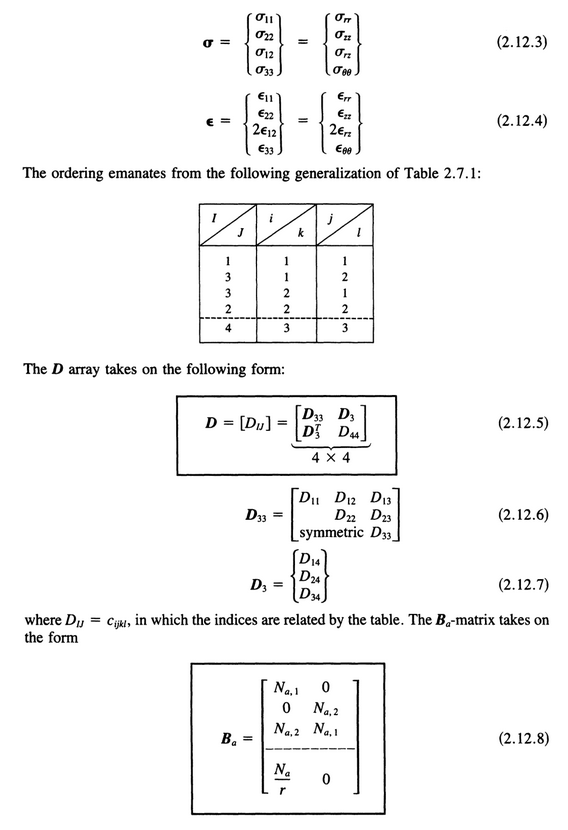
\includegraphics[width=10cm]{images/axisymmetry/hughes1}
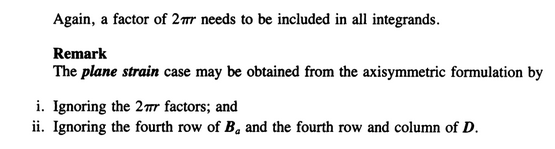
\includegraphics[width=10cm]{images/axisymmetry/hughes2}\\
{\captionfont Taken from pages 101 of \fullcite{hugh}.}
\end{center}


Also check page 469 of Gresho \& Sani's book, and 
see their remark on axisymmetric case for the N-S equations on page 545.

\Literature:
\begin{itemize}
\item \fullcite{ruas03}
\item \fullcite{leli12} 
\end{itemize}






 %----------------------

\newpage %%%%%%%%%%%%%%%%%%%%%%%%%%%%%%%%%%%%%%%%%%%%%%%%%%%%%%%%%%%%%%%%%%%%%%%%%%%%%%%%%%%%%%%%%%
\section{Mappings \& Jacobians \label{ss:mappings}} \begin{flushright} {\tiny {\color{gray} mappings.tex}} \end{flushright}
%~~~~~~~~~~~~~~~~~~~~~~~~~~~~~~~~~~~~~~~~~~~~~~~~~~~~~~~~~~~~~~~~~~~~~~~~~~~~~~~~~~~~~~~~~~~~~~~~~~

\index{general}{Isoparametric}
\index{general}{Subparametric} 
\index{general}{Superparametric}

The name {\sl isoparametric} derives from the fact that the same ('iso') 
functions are used as basis functions and for the mapping to the reference element.

More generally, if $n_e$ denotes the number of nodes of an element and $n_g$ denotes the 
number of nodes describing the geometry of the element, 
then the element is termed {\sl subparametric} when $n_g<n_e$ and 
{\sl superparametric} when $n_g>n_e$.

%...........................................
\subsubsection{Linear mapping on a triangle}

\begin{verbatim}
2
|\     s
| \    |_r
|  \
3===1
\end{verbatim}

Let us assume that the coordinates of the vertices are 
$(x_1,y_1)$,  
$(x_2,y_2)$, and 
$(x_3,y_3)$.
The coordinates inside the reference element are $(r,s)$ with 
$0\le r \le 1$ and $0 \le s \le 1$. We then simply have the 
following relationship, i.e. any point of the reference element 
can be mapped to the physical triangle as follows:
\begin{eqnarray}
x&=& r x_1 + s x_2 + (1-r-s) x_3 \\
y&=& r y_1 + s y_2 + (1-r-s) y_3 
\end{eqnarray} 
Note that the functions $r$, $s$ and $1-r-s$ are in fact the 
$P_1$ basis functions (see Section~\ref{ss:p1}).
There is also an inverse map, which is easily computed:
\begin{eqnarray}
r&=& \frac{(y_2-y_3)(x-x_3)-(x_2-x_3)(y-y_3)}{(x_1-x_3)(y_2-y_3)-(y_1-y_3)(x_2-x_3)} \\
s&=& \frac{-(y_1-y_3)(x-x_3)+(x_1-x_3)(y-y_3)}{(x_1-x_3)(y_2-y_3)-(y_1-y_3)(x_2-x_3)} 
\end{eqnarray} 
\begin{remark}
The denominator will not vanish, because it is a multiple of the area of the 
triangle. If the three points
are distinct then the area cannot be zero.
\end{remark}

%................................................
\subsubsection{Bilinear mapping on a quadrilateral}

The \index{general}{reference element} reference element 
is in the $(r,s)$ space. It is a square of size $2\times2$ 
centered around the origin, i.e. $(r,s)\in[-1,1]\times[-1,1]$. 
We wish to map it to the quadrilateral in the $(x,y)$ space 
(and vice versa):

\begin{center}
\includegraphics[width=8cm]{images/mappings/bilinear/mapping_bilinear.png}
\end{center}

The coordinates of the vertices are 
$(x_1,y_1)$, $(x_2,y_2)$, $(x_3,y_3)$ and $(x_4,y_4)$.
We then simply have the 
following relationship, i.e. any point of the reference element 
can be mapped to the physical quadrilateral as follows:
\begin{eqnarray}
x&=& \bN_1(r,s) x_1 + \bN_2(r,s) x_2 + \bN_3(r,s) x_3 + \bN_4(r,s) x_4 \\
y&=& \bN_1(r,s) y_1 + \bN_2(r,s) y_2 + \bN_3(r,s) y_3 + \bN_4(r,s) y_4 
\end{eqnarray} 
where the $Q_1$ basis functions $\bN_i(r,s)$ are defined in Section~\ref{sec:elts1D}.

In the following example the program randomly generates 10000 points 
inside the reference 
element and computes their mapping into the $(x,y)$ space. 

\begin{lstlisting}
x1=-1 ; y1=-2
x2=3  ; y2=-1
x3=2  ; y3=2
x4=-3 ; y4=1

npts=10000
r=np.zeros(npts,dtype=np.float64)   
s=np.zeros(npts,dtype=np.float64)   
x=np.zeros(npts,dtype=np.float64)   
y=np.zeros(npts,dtype=np.float64)   

for i in range(0,npts):
    # compute random r,s coordinates
    r[i]=random.uniform(-1.,+1)
    s[i]=random.uniform(-1.,+1)
    # compute basis function values at r,s
    N1=0.25*(1-r[i])*(1-s[i])
    N2=0.25*(1+r[i])*(1-s[i])
    N3=0.25*(1+r[i])*(1+s[i])
    N4=0.25*(1-r[i])*(1+s[i])
    # compute x,y coordinates
    x[i]=N1*x1+N2*x2+N3*x3+N4*x4
    y[i]=N1*y1+N2*y2+N3*y3+N4*y4

np.savetxt('rs.ascii',np.array([r,s]).T)
np.savetxt('xy.ascii',np.array([x,y]).T)
\end{lstlisting}

\begin{center}
\includegraphics[width=7cm]{images/mappings/bilinear/rs.pdf}
\includegraphics[width=7cm]{images/mappings/bilinear/xy.pdf}
\end{center}

There is also an inverse map, which is not so easily computed (see Section~\ref{sec:amiin}).
However, if the quadrilateral in the $(x,y)$ space is a rectangle of size $(h_x,h_y)$, 
the inverse mapping is trivial:
\begin{eqnarray}
r&=&\frac{x-x_1}{x_2-x_1} \\
s&=&\frac{y-y_1}{y_4-y_1} 
\end{eqnarray}
Also in the case of rectangular elements of size $(h_x,h_y)$
the basis functions can easily be written as functions of $(x,y)$:
\begin{eqnarray}
\bN_1(x,y) &=& \left( \frac{x_3 -x }{h_x}  \right) \left( \frac{y_3 -y }{h_y}  \right) \nn\\
\bN_2(x,y) &=& \left( \frac{x - x_1}{h_x}  \right) \left( \frac{y_3 -y }{h_y}  \right) \nn\\
\bN_3(x,y) &=& \left( \frac{x - x_1}{h_x}  \right) \left( \frac{y - y_1}{h_y}  \right) \nn\\
\bN_4(x,y) &=& \left( \frac{x_3 -x }{h_x}  \right) \left( \frac{y - y_1}{h_y}  \right) \nn 
\end{eqnarray}
On the one hand, any variable defined on the element can be approximated using the basis functions:
\begin{equation}
f^h(r,s)=\sum_i \bN_i(r,s) f_i.
\end{equation}
If we treat the coordinate variables $x$ and $y$ themselves as functions, 
then the basis functions can be used to construct the mapping:
\begin{equation}
x(r,s)=\sum_i \bN_i(r,s) x_i 
\qquad
y(r,s)=\sum_i \bN_i(r,s) y_i,  \label{eqxy}
\end{equation}
leading to write
\begin{eqnarray}
\frac{\partial x}{\partial r} &=& \sum_i \frac{\partial \bN_i}{\partial r} x_i \\
\frac{\partial x}{\partial s} &=& \sum_i \frac{\partial \bN_i}{\partial s} x_i \\
\frac{\partial y}{\partial r} &=& \sum_i \frac{\partial \bN_i}{\partial r} y_i \\
\frac{\partial y}{\partial s} &=& \sum_i \frac{\partial \bN_i}{\partial s} y_i 
\end{eqnarray}
On the other hand we also have 
\begin{eqnarray}
\frac{\partial f}{\partial r} &=&
\frac{\partial f}{\partial x}\frac{\partial x}{\partial r}
+\frac{\partial f}{\partial y}\frac{\partial y}{\partial r} \\
\frac{\partial f}{\partial s} &=&
\frac{\partial f}{\partial x}\frac{\partial x}{\partial s}
+\frac{\partial f}{\partial y}\frac{\partial y}{\partial s}
\end{eqnarray}
or in matrix form:
\begin{equation}
\left(
\begin{array}{c}
\frac{\partial f}{\partial r} \\ \\
\frac{\partial f}{\partial s}
\end{array}
\right)
=
\underbrace{
\left(
\begin{array}{cc}
\frac{\partial x}{\partial r} & \frac{\partial y}{\partial r} \nonumber\\ \\
\frac{\partial x}{\partial s} & \frac{\partial y}{\partial s} \nonumber
\end{array}
\right)
}_{\bm J}
\cdot
\left(
\begin{array}{c}
\frac{\partial f}{\partial x} \\ \\
\frac{\partial f}{\partial y}
\end{array}
\right)
\end{equation}
where ${\bm J}$ is called the Jacobian of the transformation
By inverting the Jacobian matrix, the desired derivatives with respect to $x$
and $y$ can be obtained:

We have:
\[
\left(
\begin{array}{c}
\frac{\partial f}{\partial x} \\ \\
\frac{\partial f}{\partial y}
\end{array}
\right)
=
{\bm J}^{-1} \cdot 
\left(
\begin{array}{c}
\frac{\partial f}{\partial r} \\ \\
\frac{\partial f}{\partial s}
\end{array}
\right)
\]
The inverse of the Jacobian matrix can be simply obtained in 
2D (Cramer's rule for $2\times2$ matrices\footnote{\url{https://en.wikipedia.org/wiki/Cramers_rule}}):
\[
{\bm J}^{-1} = \frac{1}{|{\bm J}|} 
\left(
\begin{array}{cc}
\frac{\partial y}{\partial s} & -\frac{\partial y}{\partial r} \nonumber\\ \\
-\frac{\partial x}{\partial s} & \frac{\partial x}{\partial r} \nonumber
\end{array}
\right)
\]
The presence of the determinant in the denominator implies that it cannot 
be zero anywhere, or in other words: the mapping is not valid if $|{\bm J}|$
is zero anywhere over the element.

\begin{remark}
\textcite{hua90} (1990) has published analytical inverse transformation 
for quadrilateral isoparametric elements, i.e. how to compute ${\bm J}^{-1}$ 
as a function of space coordinates and not just at the quadrature points. 
\end{remark}

Let us look at this by means of a simple example and let us consider the following 
element:
\begin{center}
\includegraphics[width=4cm]{images/mappings/fournode/ex1}
\end{center}
Then a $Q_1$ mapping yields:
\begin{eqnarray}
x(r,s) &=& \sum_i \bN_i(r,s) x_i = \bN_2 + 2\bN_3 = \frac{1}{4} (3+3r+ s+rt) \nn\\
y(r,s) &=& \sum_i \bN_i(r,s) y_i = 2\bN_3 + \bN_4 = \frac{1}{4} (3+r+ 3s+rt) 
\end{eqnarray}
The Jacobian matrix is then
\begin{equation}
{\bm J} = 
\left(
\begin{array}{cc}
\frac{\partial x}{\partial r} & \frac{\partial y}{\partial r} \nonumber\\ \\
\frac{\partial x}{\partial s} & \frac{\partial y}{\partial s} \nonumber
\end{array}
\right)
=
\frac{1}{4}
\left(
\begin{array}{cc}
3+s & 1+s \\
1+r & 3+r
\end{array}
\right)
\end{equation}
and its determinant is 
\begin{equation}
|{\bm J}|=\frac{1}{4} [(3+s)(3+r)-(1+s)(1+r)]=\frac{1}{2}+\frac{1}{8}r+\frac{1}{8}s
\end{equation}
It is clear that $|{\bm J}|>0$ for $-1\leq r \leq +1$ and $-1\leq s \leq +1$. 

Let us now consider another example, the following element:
\begin{center}
\includegraphics[width=3.5cm]{images/mappings/fournode/ex2}
\end{center}
It follows that
\begin{eqnarray}
x(r,s) &=& \sum_i \bN_i(r,s) x_i = \frac{1}{4}(1+r)(7+5s) \\ 
y(r,s) &=& \sum_i \bN_i(r,s) y_i = \frac{1}{4}(17+5r+7s-5rs)
\end{eqnarray}
and the determinant:
\[
|{\bm J}|=\frac{3}{2}-\frac{15r}{4}+\frac{15s}{4}
\]
is zero for $r-s=2/5$. This mapping is invalid!

\begin{remark}
Problems also arise when the Jacobian matrix is nearly singular due to round-off errors.
To avoid problems linked to badly shaped elements, it is recommended that the inside
angles of an element are larger than $15\degree$ and less than $165\degree$.
\end{remark}

From Eq.~\eqref{eqxy}, we can also write:
\begin{eqnarray}
dx &=& \frac{\partial x}{\partial r} dr + \frac{\partial x}{\partial s} ds \\
dy &=& \frac{\partial y}{\partial r} dr + \frac{\partial y}{\partial s} ds 
\end{eqnarray}
or, 
\begin{equation}
\left(
\begin{array}{c}
dx \\ dy
\end{array}
\right)
={\bm J}\cdot
\left(
\begin{array}{c}
dr \\ ds
\end{array}
\right)
\end{equation}
This means that integrating over the 'real' element in $(x,y)$ space
can be simply done by integrating of the reference element in the 
$(r,s)$ space. This is the cornerstone of most of the implementation of the 
Finite Element Method, the second integral being carried out by means 
of the Gauss-Legendre quadrature.

\begin{equation}
\iint_{\Omega_e} ... \; dx dy = \int_{-1}^{+1} \int_{-1}^{+1} ...|{\bm J}| \; dr ds
\end{equation}


%.................................................................
\subsubsection{Biquadratic mapping of a straight-edge face $Q_2$ element }

\begin{center}
\includegraphics[width=8cm]{images/mappings/biquadratic/mapping1}
\end{center}

The reference element now contains 9 nodes: 1,3,7,9 are the corners, nodes
2,4,6,8 are the mid-face points and node 5 is in the middle\footnote{Note that 
this numbering is quite arbitrary}.
The mapping from the $(r,s)$ space to the $(x,y)$ space is then as follows:

\begin{eqnarray}
\left(
\begin{array}{c}
x(r,s) \\ y(r,s)
\end{array}
\right)
&=&
\bN_1(r,s)
\left(
\begin{array}{c}
x_1 \\ y_1
\end{array}
\right)
+
\bN_2(r,s)
\left(
\begin{array}{c}
x_2 \\ y_2
\end{array}
\right)
+
\bN_3(r,s)
\left(
\begin{array}{c}
x_3 \\ y_3
\end{array}
\right)
+
\bN_4(r,s)
\left(
\begin{array}{c}
x_4 \\ y_4
\end{array}
\right) \nonumber\\
&+&
\bN_5(r,s)
\left(
\begin{array}{c}
x_5 \\ y_5
\end{array}
\right)
+
\bN_6(r,s)
\left(
\begin{array}{c}
x_6 \\ y_6
\end{array}
\right)
+
\bN_7(r,s)
\left(
\begin{array}{c}
x_7 \\ y_7
\end{array}
\right)
+
\bN_8(r,s)
\left(
\begin{array}{c}
x_4 \\ y_8
\end{array}
\right) \nonumber\\
&+&
\bN_9(r,s)
\left(
\begin{array}{c}
x_9 \\ y_9
\end{array}
\right) 
\nonumber
\end{eqnarray}
where the $Q_2$ basis functions have been obtained in Section~\ref{ss:q22d}:
\begin{eqnarray}
\bN_1(r,t)&=& 0.5r(r-1)  0.5t(t-1) \nonumber\\
\bN_2(r,t)&=&      (1-r^2)  0.5t(t-1) \nonumber\\
\bN_3(r,t)&=& 0.5r(r+1)  0.5t(t-1) \nonumber\\
\bN_4(r,t)&=& 0.5r(r-1)       (1-t^2) \nonumber\\
\bN_5(r,t)&=&      (1-r^2)       (1-t^2) \nonumber\\
\bN_6(r,t)&=& 0.5r(r+1)       (1-t^2) \nonumber\\
\bN_7(r,t)&=& 0.5r(r-1)  0.5t(t+1) \nonumber\\
\bN_8(r,t)&=&      (1-r^2)  0.5t(t+1) \nonumber\\
\bN_9(r,t)&=& 0.5r(r+1)  0.5t(t+1) \nonumber
\end{eqnarray}


\begin{lstlisting}
x1=-1                 ; y1=-2
x3=3                  ; y3=-1
x9=2                  ; y9=2
x7=-3                 ; y7=1
x2=0.5*(x1+x3)        ; y2=0.5*(y1+y3)
x4=0.5*(x1+x7)        ; y4=0.5*(y1+y7)
x6=0.5*(x3+x9)        ; y6=0.5*(y3+y9)
x8=0.5*(x7+x9)        ; y8=0.5*(y7+y9)
x5=0.25*(x1+x3+x7+x9) ; y5=0.25*(y1+y3+y7+y9)

npts=10000
r=np.zeros(npts,dtype=np.float64)   
s=np.zeros(npts,dtype=np.float64)   
xQ1=np.zeros(npts,dtype=np.float64)   
yQ1=np.zeros(npts,dtype=np.float64)   
xQ2=np.zeros(npts,dtype=np.float64)   
yQ2=np.zeros(npts,dtype=np.float64)   

for i in range(0,npts):
    # compute random r,s coordinates
    r[i]=random.uniform(-1.,+1)
    s[i]=random.uniform(-1.,+1)
    # compute Q2 basis function values at r,s
    N1= 0.5*r[i]*(r[i]-1.) * 0.5*s[i]*(s[i]-1.)
    N2=       (1.-r[i]**2) * 0.5*s[i]*(s[i]-1.)
    N3= 0.5*r[i]*(r[i]+1.) * 0.5*s[i]*(s[i]-1.)
    N4= 0.5*r[i]*(r[i]-1.) *       (1.-s[i]**2)
    N5=       (1.-r[i]**2) *       (1.-s[i]**2)
    N6= 0.5*r[i]*(r[i]+1.) *       (1.-s[i]**2)
    N7= 0.5*r[i]*(r[i]-1.) * 0.5*s[i]*(s[i]+1.)
    N8=       (1.-r[i]**2) * 0.5*s[i]*(s[i]+1.)
    N9= 0.5*r[i]*(r[i]+1.) * 0.5*s[i]*(s[i]+1.)
    # compute x,y coordinates
    xQ2[i]=N1*x1+N2*x2+N3*x3+N4*x4+N5*x5+N6*x6+N7*x7+N8*x8+N9*x9
    yQ2[i]=N1*y1+N2*y2+N3*y3+N4*y4+N5*y5+N6*y6+N7*y7+N8*y8+N9*y9
    # compute Q1 basis function values at r,s
    N1=0.25*(1-r[i])*(1-s[i])
    N2=0.25*(1+r[i])*(1-s[i])
    N3=0.25*(1+r[i])*(1+s[i])
    N4=0.25*(1-r[i])*(1+s[i])
    # compute x,y coordinates
    xQ1[i]=N1*x1+N2*x3+N3*x9+N4*x7
    yQ1[i]=N1*y1+N2*y3+N3*y9+N4*y7

np.savetxt('rs.ascii',np.array([r,s]).T)
np.savetxt('xyQ1.ascii',np.array([xQ1,yQ1]).T)
np.savetxt('xyQ2.ascii',np.array([xQ2,yQ2]).T)
\end{lstlisting}

The code is available in {\tt /images/mappings/biquadratic}
Note that the coordinates of point 5 are defined being those of the barycenter
of the quadrilateral. More on this choice later.

\begin{center}
a)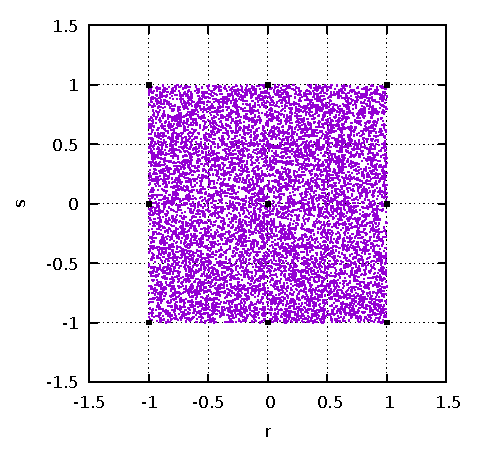
\includegraphics[width=5.6cm]{images/mappings/biquadratic/rs.pdf}
b)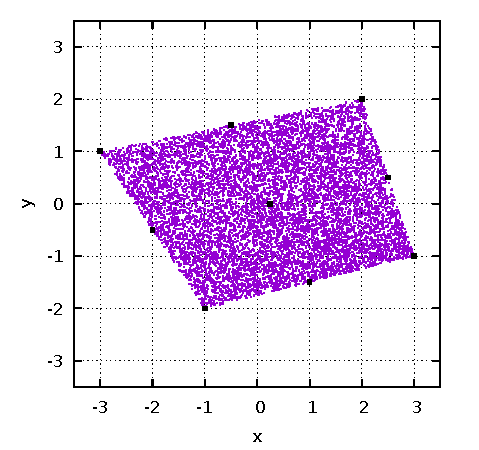
\includegraphics[width=5.6cm]{images/mappings/biquadratic/xyQ1.pdf}
c)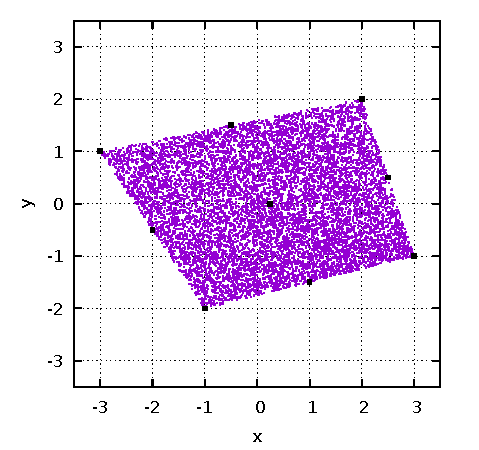
\includegraphics[width=5.6cm]{images/mappings/biquadratic/xyQ2.pdf}\\
{\captionfont a) 10,000 random points in the reference element; 
b,c) image of these points by means of a bilinear and biquadratic mapping 
respectively.\\ When the sides of the element
are straight we see that a $Q_1$ mapping is sufficient.}
\end{center}

%.................................................................
\subsubsection{Biquadratic mapping of a not-so straight-line face $Q_2$ element }

We now carry out the same exercise as before but nodes 2 and 8 are no more 
in the middle of nodes 1-3 and 7-9 respectively.
The code is available in {\tt /images/mappings/biquadratic2}.

\begin{center}
a)\includegraphics[width=4.5cm]{images/mappings/biquadratic2/rs.pdf}
b)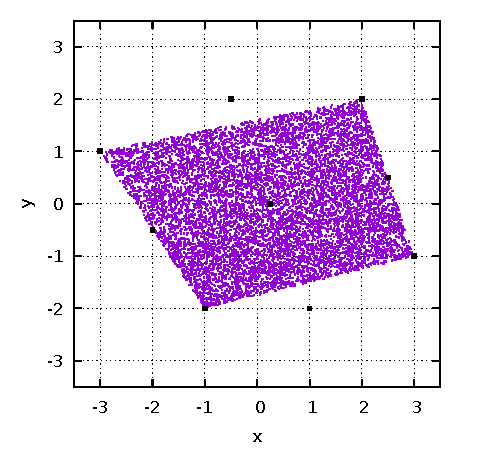
\includegraphics[width=4.5cm]{images/mappings/biquadratic2/xyQ1.pdf}
c)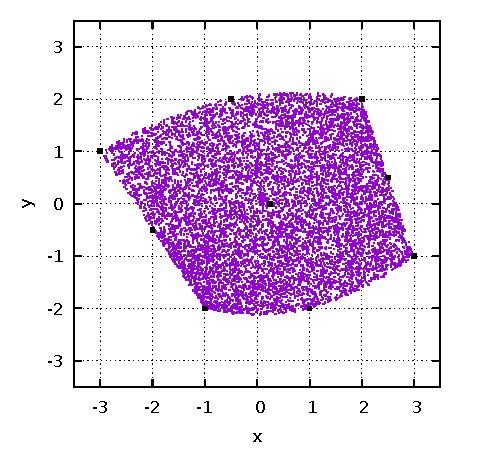
\includegraphics[width=4.5cm]{images/mappings/biquadratic2/xyQ2.pdf}\\
{\captionfont a) 10,000 random points in the reference element; 
b,c) image of these points by means of a bilinear and biquadratic mapping 
respectively.} 
\end{center}

In this case we see that 
the $Q_2$ mapping manages to better capture the 'real' shape of the element.
Since nodes 2 and 8 have moved, we could now ask ourselves 
where we should place node 5? In this example we set it as follows
but it is somewhat arbitrary.
\begin{lstlisting}
x5=(x1+x2+x3+x4+x6+x7+x8+x9)/8. 
y5=(y1+y2+y3+y4+y6+y7+y8+y9)/8.
\end{lstlisting}
We will come back to this later.

%.......................................................................
\subsubsection{Bilinear, biquadratic and bicubic mapping in an annulus }

In the light of what precedes, we can now ask ourselves how this translates to 
a real geodynamic case. Let us then consider the case of an annular domain, 
a cross section of a hollow sphere. 
When using quadrilateral elements, the mesh will look similar to this:

\begin{center}
\includegraphics[width=6cm]{images/mappings/curved/annulus_mesh}
\end{center}

We here focus on $Q_1$, $Q_2$ and $Q_3$ mappings. We single out an element, 
and arbitrarily define it as follows in polar coordinates:
\begin{lstlisting}
theta1=23./180.*np.pi
theta2=52./180.*np.pi
R1=1.
R2=1.5
\end{lstlisting}
The $Q_1$ mapping requires four points, the $Q_2$ nine points and the $Q_3$
sixteen points. 
The code used in the following is available at {\tt ./images/mappings/curved/}.
These are placed equidistantly in the $r,\theta$ coordinate
system, as shown hereunder:

\begin{center}
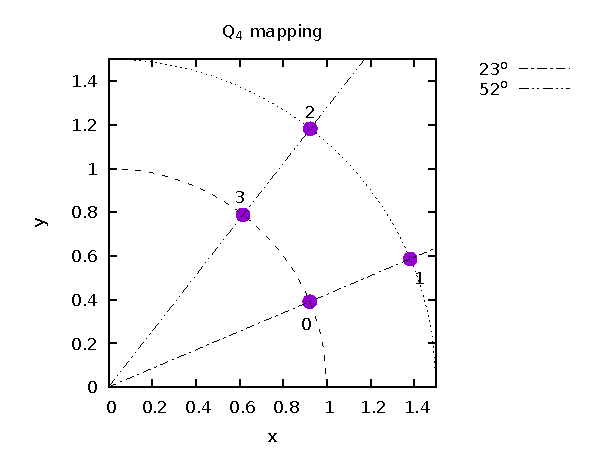
\includegraphics[width=5.7cm]{images/mappings/curved/nodesQ1.pdf}
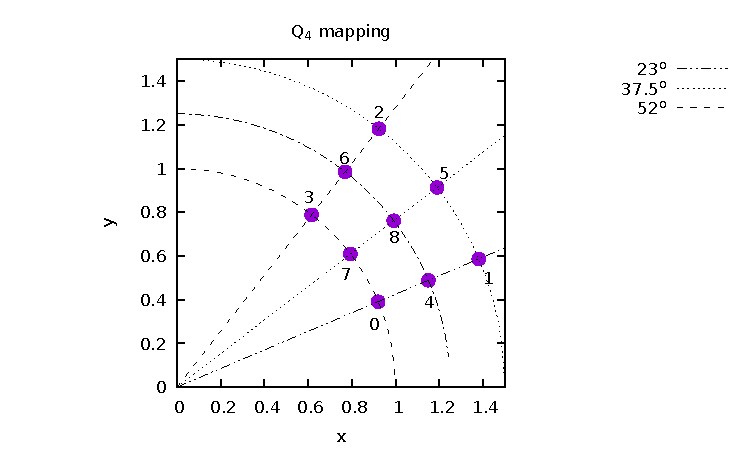
\includegraphics[width=5.7cm]{images/mappings/curved/nodesQ2.pdf}
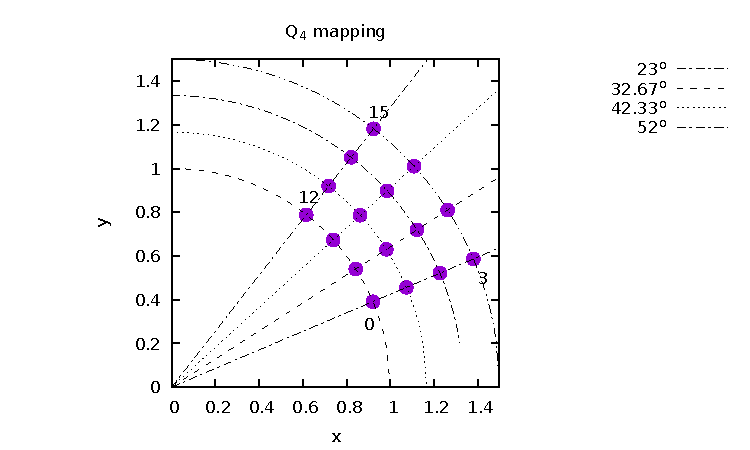
\includegraphics[width=5.7cm]{images/mappings/curved/nodesQ3.pdf}\\
{\captionfont Left to right: position of the nodes for the $Q_1$, $Q_2$ and $Q_3$ mappings.
$Q_4$ is not shown.}
\end{center}

As before, we randomly shoot 10,000 points inside the reference element 
and map these out in the $x,y$ space. Resulting swarms of points are shown 
in the following figures:

\begin{center}
\includegraphics[width=5.7cm]{images/mappings/curved/xy1_keep.pdf}
\includegraphics[width=5.7cm]{images/mappings/curved/xy2_keep.pdf}
\includegraphics[width=5.7cm]{images/mappings/curved/xy3_keep.pdf}\\
{\captionfont Left to right: position of the mapped points for the $Q_1$, $Q_2$ and $Q_3$ mappings.
$Q_4$ is not shown.}
\end{center}

The image of a square with a $Q_1$ mapping is obviously a quadrilateral
so that it looks like quite a few points land outside of the domain $R_1\leq r\leq R_2$.
Note that points are well within $23\degree \leq \theta \leq 52\degree$, which can 
simply be explained by the fact that the faces of the element joining $R_1$
to $R_2$ are straight lines.

However, it looks like the biquadratic and bicubic mappings are doing a much better 
job at mapping the region of space $R_1\leq r\leq R_2$. In order to characterise 
this better, we now place 10,000 points on the bottom face of 
the reference element (i.e. $s=-1$)
and once again compute their coordinates in the the $x,y$ space:

\begin{center}
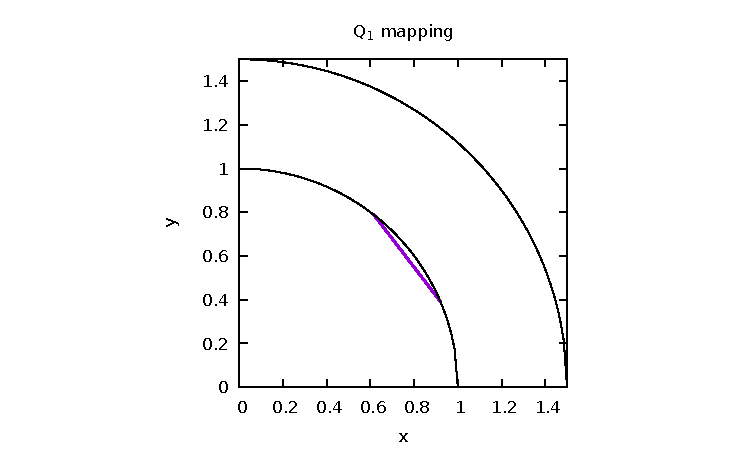
\includegraphics[width=8cm]{images/mappings/curved/xy1.pdf}
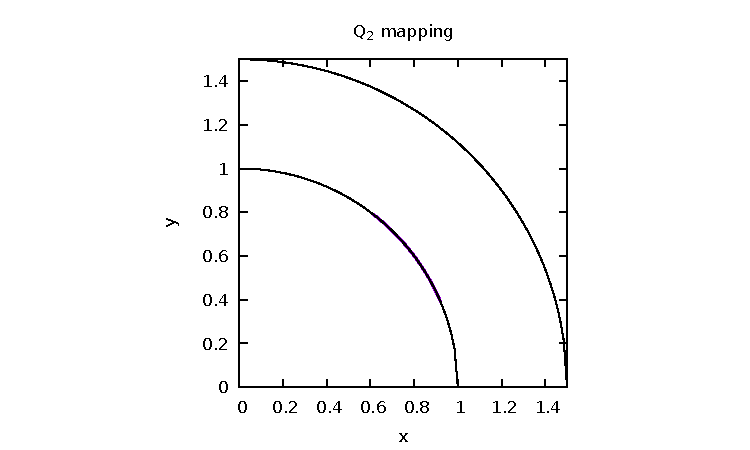
\includegraphics[width=8cm]{images/mappings/curved/xy2.pdf}\\
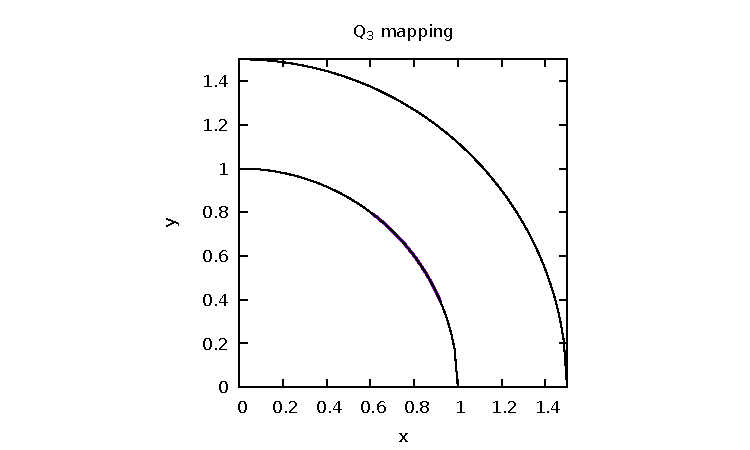
\includegraphics[width=8cm]{images/mappings/curved/xy3.pdf}
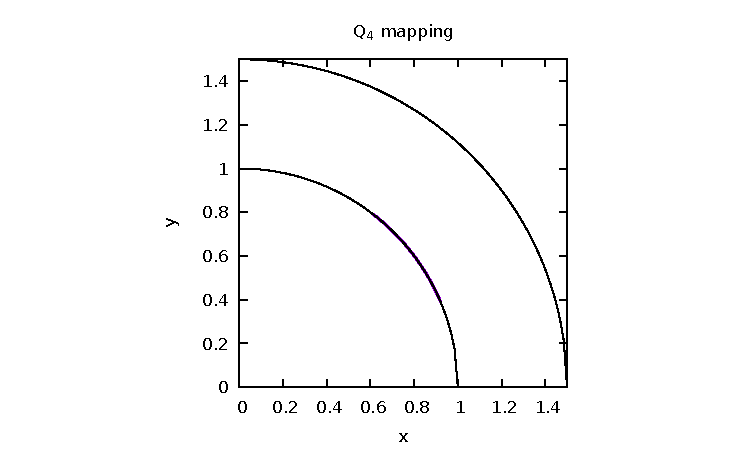
\includegraphics[width=8cm]{images/mappings/curved/xy4.pdf}\\
{\captionfont Position of the mapped points for the $Q_1$, $Q_2$, $Q_3$ and $Q_4$ mappings.}
\end{center}

For each point $i$ we now compute the distance $r_i$ 
to the origin, which, if the 
mapping was perfect, would be exactly equal to $R_1=1$. 
On the following plots are shown the error $r_i-1$ for all 
points, from $r=-1$ to $r=+1$.

\begin{center}
\includegraphics[width=8cm]{images/mappings/curved/innerline_error_Q1mapping.pdf}
\includegraphics[width=8cm]{images/mappings/curved/innerline_error_Q2mapping.pdf}\\
\includegraphics[width=8cm]{images/mappings/curved/innerline_error_Q3mapping.pdf}
\includegraphics[width=8cm]{images/mappings/curved/innerline_error_Q4mapping.pdf}\\
{\captionfont Radius error of the mapped points for the $Q_1$, $Q_2$, $Q_3$ and $Q_4$ mappings.}
\end{center}

We see that the amplitude of the error decreases with the order of the mapping used, 
which is why for instance \aspect uses a $Q_4$ mapping by default\footnote{I find it also quite striking 
that the $Q_4$ mapping outperforms the $Q_3$ one by two orders of magnitude...}.
Actually, in this particular case, the equation which describes the circle is not a 
polynomial so that no high-order mapping will ever be able to {\it exactly} 
represent the curved boundary of the element!

Another interesting point to keep in mind is that the location of the quadrature points
in the $x,y$ space is also determined by the mapping used, which can have consequences
on the accuracy of the integration and it will be reflected (for instance) on the 
error convergence rate.

As already mentioned previously, 
the coordinates of the nodes of the element in the $x,y$ are 
uniquely determined when they are on the convex hull of the element (
for instance nodes 0-7 for $Q_2$) but we need to choose the position 
of the last nodes which are inside the element. Unfortunately, this choice is 
not neutral. 

Finally, we can explore the importance of the mapping in combination with 
numerical quadrature. For each mapping we compute the area of the element
by means of a 3x3, 4x4 or 5x5 quadrature.

\begin{verbatim}
**********Q1*********
nqperdim= 3 0.3030060126539606 rel. error -0.04215361698430029
nqperdim= 4 0.3030060126539606 rel. error -0.04215361698430012 ~ 4%
nqperdim= 5 0.3030060126539606 rel. error -0.04215361698430012
**********Q2*********
nqperdim= 3 0.3162980025394154 rel. error -0.00013569026611326453
nqperdim= 4 0.3162980025394155 rel. error -0.00013569026611308905 ~ 0.01%
nqperdim= 5 0.3162980025394154 rel. error -0.00013569026611326453
**********Q3*********
nqperdim= 3 0.3163472223929359 rel. error 1.9900899402587318e-05
nqperdim= 4 0.316347222392936  rel. error 1.9900899402938278e-05 ~ 0.002%
nqperdim= 5 0.316347222392936  rel. error 1.9900899402938278e-05
**********Q4*********
nqperdim= 3 0.3163409410866220 rel. error 4.477021014282521e-08
nqperdim= 4 0.3163409541901677 rel. error 8.619243716974044e-08 ~ 0.000008%
nqperdim= 5 0.316340954190168  rel. error 8.619243804713484e-08
\end{verbatim}

Here again the $Q_4$ mapping makes quite the difference. 

\newpage

%..................................................................
\subsubsection{Biquadratic mapping - the middle node conundrum}

Python code at {\tt images/mappings/biquadratic3}.

As mentioned before, unless the element is a straight-edge quadrilateral, 
determining the (best) position of the middle node is not trivial. Or is it?


\begin{verbatim}

4--7--3
|     |
8  9  6   (reference element)
|     |
1--5--2

\end{verbatim}

We will here consider 5 different elements:

\begin{center}
\includegraphics[width=3.5cm]{images/mappings/biquadratic3/elt0/element0}
\includegraphics[width=3.5cm]{images/mappings/biquadratic3/elt1/element1}
\includegraphics[width=3.5cm]{images/mappings/biquadratic3/elt2/element2}
\includegraphics[width=3.5cm]{images/mappings/biquadratic3/elt3/element3}
\includegraphics[width=3.5cm]{images/mappings/biquadratic3/elt4/element4}\\
{\captionfont From left to right: element 0,1,2,3,4.}
\end{center}

We can think of multiple ways to come up with the 'center' of the element, 
i.e. the location of point I.

\begin{itemize}
\item {\python center=0}: 
\[
x_9=(x_1+x_2+x_3+x_4)/4 
\qquad
y_9=(y_1+y_2+y_3+y_4)/4
\]

\item {\python center=1}: 
\[
x_9=(x_1+x_2+x_3+x_4+x_5+x_6+x_7+x_8)/8 
\qquad
y_9=(y_1+y_2+y_3+y_4+y_5+y_6+y_7+y_8)/8
\]
\item {\python center=2}:
\[
x_9=(x_1+x_2+x_3+x_4+3x_5+3x_6+3x_7+3x_8)/16. 
\qquad
y_9=(y_1+y_2+y_3+y_4+3y_5+3y_6+3y_7+3y_8)/16.
\]
\item {\python center=3}: (only element=4)
\[
x_9=\frac12(R_1+R_2)\cos(3\pi/8) 
\qquad
y_9=\frac12(R_1+R_2)\sin(3\pi/8)
\]
\item {\python center=4}: I is the center of mass. 
The element is defined by $R_1<r<R_2$ and $\theta_1<\theta<\theta_2$.

We need to compute\footnote{\url{https://en.wikipedia.org/wiki/Center_of_mass}}
\begin{eqnarray}
\vec{R} 
&=&\frac{1}{M} \int \vec{r} \rho(\vec r) dV \nn\\
&=&\frac{1}{M} \rho_0 \int \vec{r} dV\nn\\
&=&\frac{1}{M} \frac{M}{V} \int \vec{r} dV\nn\\
&=&\frac{1}{V} \int \vec{r} dV\nn\\
&=&\frac{1}{V} \int \left(\begin{array}{c} x \\ y \end{array}\right)  dV\nn\\
&=&\frac{1}{V} \int \left(\begin{array}{c} r \cos \theta \\ r \sin\theta \end{array}\right)dV\nn\\
&=&\frac{1}{V} \int_{R_1}^{R_2} \int_{\theta_1}^{\theta_2} \left(\begin{array}{c} r \cos \theta 
\\ r \sin\theta \end{array}\right)  r dr d\theta\nn\\
&=&\frac{1}{\frac12 (R_2^2-R_1^2) (\theta_2-\theta_1)} \frac13(R_2^3-R_1^3) 
\left(
\begin{array}{c}
\sin\theta_2-\sin\theta_1 \\
-\cos\theta_2+\cos\theta_1 
\end{array}
\right) \nn\\
&\simeq& 
\left(
\begin{array}{c}
0.5801028000103104\\
1.4004920473554983
\end{array}
\right) 
\end{eqnarray}
which corresponds to $r=1.5158816686291174$ and $\theta=67.5^o=3\pi/8$.

\item {\python center=5}: variable position
\end{itemize}


isoparametric mapping. 


At each point $(r,s)$ we compute the error $|\sum_i N_i(r,s) x_i^2 - (\sum_i N_i(r,s) x_i)^2|$.

position of edges (setting r=+- 1, s=+-1) independent of position of middle node since shape functions are zero there

area indep of position middle node ?



%....................
\paragraph{Element 0}

In this case all only {\python center=0,1,2,4} are applicable but they all 
lead to the same point I with $x_I=0,y_I=0$. This means that the position of 
quadrature points is also independent of the {\python center} parameter.
 
\begin{center}
\includegraphics[width=5.7cm]{images/mappings/biquadratic3/elt0/jcob}
\includegraphics[width=5.7cm]{images/mappings/biquadratic3/elt0/error_posx2}
\includegraphics[width=5.7cm]{images/mappings/biquadratic3/elt0/error_posy2}\\
{\captionfont 10,000 points at random.} 
\end{center}

%....................
\paragraph{Element 1}

In this case all only {\python center=0,1,2,4} are applicable but they all 
lead to the same point I with $x_I=0,y_I=0$. This means that the position of 
quadrature points is also independent of the {\python center} parameter.
 
\begin{center}
\includegraphics[width=5.7cm]{images/mappings/biquadratic3/elt1/jcob}
\includegraphics[width=5.7cm]{images/mappings/biquadratic3/elt1/error_posx2}
\includegraphics[width=5.7cm]{images/mappings/biquadratic3/elt1/error_posy2}\\
{\captionfont 10,000 points at random.} 
\end{center}


%....................
\paragraph{Element 2} .

\begin{center}
\includegraphics[width=5.7cm]{images/mappings/biquadratic3/elt2/jcob_0}
\includegraphics[width=5.7cm]{images/mappings/biquadratic3/elt2/jcob_1}
\includegraphics[width=5.7cm]{images/mappings/biquadratic3/elt2/jcob_2}\\
\includegraphics[width=5.7cm]{images/mappings/biquadratic3/elt2/error_posx2_0}
\includegraphics[width=5.7cm]{images/mappings/biquadratic3/elt2/error_posx2_1}
\includegraphics[width=5.7cm]{images/mappings/biquadratic3/elt2/error_posx2_2}\\
\includegraphics[width=5.7cm]{images/mappings/biquadratic3/elt2/error_posy2_0}
\includegraphics[width=5.7cm]{images/mappings/biquadratic3/elt2/error_posy2_1}
\includegraphics[width=5.7cm]{images/mappings/biquadratic3/elt2/error_posy2_2}\\
{\captionfont 50,000 points at random. From left to right: center=0,1,2.} 
\end{center}




%....................
\paragraph{Element 3} .

\begin{center}
\includegraphics[width=5.7cm]{images/mappings/biquadratic3/elt3/jcob_0}
\includegraphics[width=5.7cm]{images/mappings/biquadratic3/elt3/jcob_1}
\includegraphics[width=5.7cm]{images/mappings/biquadratic3/elt3/jcob_2}\\
{\captionfont 50,000 points at random. From left to right: center=0,1,2.} 
\end{center}




%....................
\paragraph{Element 4}


\begin{center}
\includegraphics[width=5.7cm]{images/mappings/biquadratic3/elt4/jcob_0}
\includegraphics[width=5.7cm]{images/mappings/biquadratic3/elt4/jcob_1}
\includegraphics[width=5.7cm]{images/mappings/biquadratic3/elt4/jcob_2}\\
\includegraphics[width=5.7cm]{images/mappings/biquadratic3/elt4/jcob_3}
\includegraphics[width=5.7cm]{images/mappings/biquadratic3/elt4/jcob_4}\\
{\captionfont 50,000 points at random. From left to right: center=0,1,2,3,4.} 
\end{center}




\begin{center}
\includegraphics[width=8.5cm]{images/mappings/biquadratic3/elt4/nodes}
\includegraphics[width=8.5cm]{images/mappings/biquadratic3/elt4/quads}\\
{\captionfont Left: position of the nodes. Right position of quadrature points with 
nqperdim=3.}
\end{center}

\begin{verbatim}

\end{verbatim}

Area does not depend on position of middle node?!




\vspace{1cm}

\Literature 
\begin{itemize}
\item \fullcite{yuhy94}
\end{itemize}








 
 %-----------------------------

\newpage %%%%%%%%%%%%%%%%%%%%%%%%%%%%%%%%%%%%%%%%%%%%%%%%%%%%%%%%%%%%%%%%%%%%%%%%%%%%%%%%%%%%%%%%%%
\section{Solving the elastic equations} 
{\large \color{orange} This will be moved to Section \ref{chapt:elasticity}}


NOW BEING REWORKED IN OVERLEAF

In what follows $\vec\upnu$ now stands for the displacement vector, i.e. 
with units of length, not velocity. 
As before, the displacement inside an element is given by 
\begin{equation}
{\vec \upnu}^h({\vec r})=\sum_{i=1}^{m_v} N_i({\vec r})\;  {\vec \upnu}_i
\label{mixed01_el}
\end{equation}
where $N_i$ are the polynomial basis functions for the displacement.
Pressure does not appear in the equations so this is not a case of 
mixed FE as for the viscous Stokes flow. 

Other notations are sometimes used for Eqs.(\ref{mixed01_el}):
\begin{equation}
u^h({\vec r}) = \vec{N} \cdot \vec{u}
\quad\quad\quad\quad
v^h({\vec r}) = \vec{N} \cdot \vec{v}
\quad\quad\quad\quad
w^h({\vec r}) = \vec{N} \cdot \vec{w}
\end{equation} 
where ${\vec \upnu}=(u,v,w)$ and $\vec{N}$ 
is the vector containing all basis functions evaluated at location ${\vec r}$:
\begin{eqnarray}
\vec{N}^v &=& \left( N_1({\vec r}),  N_2({\vec r}),  N_3({\vec r}), \dots  N_{m_v}({\vec r}) \right) \\
\vec{N}^p &=& \left( N_1^p({\vec r}),  N_2^p({\vec r}),  N_3^p({\vec r}), \dots  N_{m_p}^p({\vec r}) \right)
\end{eqnarray}
and with 
\begin{eqnarray}
\vec{u} &=& \left( u_1,  u_2,  u_3, \dots  u_{m_v} \right) \\
\vec{v} &=& \left( v_1,  v_2,  v_3, \dots  v_{m_v} \right) \\
\vec{w} &=& \left( w_1,  w_2,  w_3, \dots  w_{m_v} \right) \\
\end{eqnarray}

%............................................
\paragraph{In three dimensions} We start from
\[
{\bm \sigma} = \lambda (\vec\nabla\cdot \vec\upnu) {\bm 1}+ 2\mu {\bm \varepsilon}
\]
where $\mu$ is the shear modulus and $\lambda$ the Lam{\'e} parameter.

\begin{eqnarray}
\sigma_{xx} &=& (\lambda+2\mu)  \varepsilon_{xx} + \lambda \varepsilon_{yy} + \lambda \varepsilon_{zz} \nn\\
\sigma_{yy} &=& \lambda \varepsilon_{xx} + (\lambda+2\mu)  {\varepsilon}_{yy} + \lambda \varepsilon_{zz}\nn\\
\sigma_{zz} &=& \lambda \varepsilon_{xx} + \lambda \varepsilon_{yy} + (\lambda+2\mu)  {\varepsilon}_{zz} \nn\\
\sigma_{xy} &=& 2\mu  {\varepsilon}_{xy} \nn\\
\sigma_{xz} &=& 2\mu  {\varepsilon}_{xz} \nn\\
\sigma_{yz} &=& 2\mu  {\varepsilon}_{yz} 
\end{eqnarray}
or, 
\[
\vec\sigma =
\left(
\begin{array}{c}
\sigma_{xx}\\ 
\sigma_{yy} \\
\sigma_{zz} \\
\sigma_{xy} \\
\sigma_{xz} \\
\sigma_{yz} 
\end{array}
\right)
=
\left(
\begin{array}{cccccc}
\lambda+2\mu & \lambda & \lambda & 0 & 0 & 0 \\
\lambda & \lambda+2\mu & \lambda & 0 & 0 & 0 \\
\lambda & \lambda & \lambda+2\mu & 0 & 0 & 0 \\
0 & 0 & 0 & \mu & 0 & 0\\
0 & 0 & 0 & 0 & \mu & 0\\
0 & 0 & 0 & 0 & 0 & \mu
\end{array}
\right)
\cdot
\left(
\begin{array}{c}
\varepsilon_{xx} \\
\varepsilon_{yy} \\
\varepsilon_{zz} \\
2\varepsilon_{xy} \\
2\varepsilon_{xz} \\
2\varepsilon_{yz} 
\end{array}
\right)
=\vec\varepsilon
\]
The rest of the procedure is pretty straightforward since it follows the same 
ideas as for the mixed viscous case, except that we here build the $\K$ matrix 
only as follows:
\[
\K=\int_{\Omega_e} {\bm B}^T \cdot {\bm D} \cdot {\bm B} \; dV 
\]




%............................................
\paragraph{In two dimensions} The above relationships simplify to 
\begin{eqnarray}
\sigma_{xx} &=& (\lambda+2\mu)  \varepsilon_{xx} + \lambda \varepsilon_{yy} \\
\sigma_{yy} &=& \lambda \varepsilon_{xx} + (\lambda+2\mu)  \dot{\varepsilon}_{yy} \\
\sigma_{xy} &=& 2\mu  \dot{\varepsilon}_{xy} 
\end{eqnarray}
so 

\[
\vec\sigma =
\left(
\begin{array}{c}
\sigma_{xx}\\ 
\sigma_{yy} \\
\sigma_{xy} 
\end{array}
\right)
=
\left(
\begin{array}{ccc}
\lambda+2\mu & \lambda & 0 \\ 
\lambda & \lambda+2\mu & 0 \\
0 & 0 & \mu 
\end{array}
\right)
\cdot
\left(
\begin{array}{c}
\varepsilon_{xx} \\
\varepsilon_{yy} \\
2\varepsilon_{xy} 
\end{array}
\right)
=\vec\varepsilon
\]







%%%%%%%%%%%%%%%%%%%%%%%%%%%%%%%%%%%%%%%%%%%%%%%%%%%%%%%%%%%%%%%%%%%%%%
\subsubsection{The axisymmetric case} \label{ss:fem_elast_axis}


We start from 
\begin{equation}
{\bm \sigma} = \lambda \vec\nabla\cdot\vec{u}\;  {\bm 1}
+2 \mu {\bm \varepsilon}(\vec{u})
\label{eq:elast_as}
\end{equation}
In cylindrical coordinates the velocity gradient is given by 
\[
\vec\nabla \vec{u}  =
\left(
\begin{array}{ccc}
{\partial \, u_r \over \partial \, r} &
{1 \over r} {\partial \, u_r \over \partial \, \theta} - {u_{\theta} \over r} &
{\partial \, u_r \over \partial z} \\
\\
{\partial \, u_{\theta} \over \partial \, r} &
{1 \over r} {\partial \, u_{\theta} \over \partial \, \theta} + {u_r \over r} &
{\partial \, u_{\theta} \over \partial z} \\
\\
{\partial \, u_{z} \over \partial \, r} &
{1 \over r} {\partial \, u_{z} \over \partial \, \theta} &
{\partial \, u_{z} \over \partial z}
\end{array}
\right)
\]
In the case of axisymmetry, and in this case symmetry about the $z$ axis, there is invariance with respect to the rotation around the axis so stresses and other quantities are independent of the $\theta$ coordinate, or simply put $\partial_\theta \rightarrow 0$.
The velocity gradient simplifies to:
\[
\vec\nabla \vec{u}  =
\left(
\begin{array}{ccc}
{\partial \, u_r \over \partial \, r} &
- {u_{\theta} \over r} &
{\partial \, u_r \over \partial z} \\
\\
{\partial \, u_{\theta} \over \partial \, r} &
{u_r \over r} &
{\partial \, u_{\theta} \over \partial z} \\
\\
{\partial \, u_{z} \over \partial \, r} &
0 &
{\partial \, u_{z} \over \partial z}
\end{array}
\right)
\]
Also, it follows logically that $u_\theta=0$ so that ultimately:
\[
\vec\nabla \vec{u}  =
\left(
\begin{array}{ccc}
\frac{\partial u_r}{\partial r} & 0 & {\partial  u_r \over \partial z} \\\\
0 & {u_r \over r} & 0 \\ \\
{\partial u_{z} \over \partial  r} & 0 & {\partial  u_{z} \over \partial z}
\end{array}
\right)
\]
and the strain tensor is then given by 
\begin{equation}
\label{eq:strain_ass} 
{\bm \varepsilon}(\vec{u})
=\frac12\left(\vec\nabla \vec{u}+\vec\nabla \vec{u}^T\right)
=
\left(
\begin{array}{ccc}
{\partial \, u_r \over \partial \, r} &
0 &
\frac12({\partial u_{z} \over \partial r} + {\partial u_r \over \partial z}) \\ \\
0 & {u_r \over r} & 0 \\ \\
\frac12({\partial u_{z} \over \partial r} + {\partial u_r \over \partial z} ) & 0 & {\partial u_{z} \over \partial z} 
\end{array}
\right)
\end{equation}
The term $\vec\nabla \cdot \vec{u}$ is simply the trace of ${\bm \varepsilon}(\vec{u})$ so 
\[
\vec\nabla \cdot \vec{u}
= {\partial u_r \over \partial r} +{u_r \over r}
+{\partial u_{z} \over \partial z}
\]
Finally the full stress tensor is then 
\begin{eqnarray}
{\bm \sigma}
&=&
\left(
\begin{array}{ccc}
\lambda({\partial  u_r \over \partial  r}
+{u_r \over r} +{\partial  u_{z} \over \partial z}) +
2\mu {\partial  u_r \over \partial  r} &
0 & \mu({\partial u_{z} \over \partial  r} + {\partial u_r \over \partial z} ) \\
\\
0 & \lambda({\partial u_r \over \partial r}
+{u_r \over r} +{\partial u_{z} \over \partial z}) + 2\mu{u_r \over r} & 0 \\
\\
\mu({\partial u_{z} \over \partial r} + {\partial u_r \over \partial z} )&0 & \lambda({\partial u_r \over \partial r}
+{u_r \over r} +{\partial u_{z} \over \partial z}) +
2\mu{\partial  u_{z} \over \partial z}
\end{array}
\right) \nonumber\\ \nonumber\\
&=&
\left(
\begin{array}{ccc}
(\lambda+ 2\mu) {\partial u_r \over \partial r}
+\lambda ({u_r \over r} +{\partial  u_{z} \over \partial z})  &
0 &
\mu({\partial u_{z} \over \partial  r} + {\partial u_r \over \partial z} ) \\
\\
0 &
(\lambda+2\mu) \frac{u_r}{r}
+ \lambda({\partial  u_r \over \partial r}
+{\partial u_{z} \over \partial z}) &
0 \\
\\
\mu({\partial u_{z} \over \partial r} + {\partial u_r \over \partial z} ) &
0 &
(\lambda+2\mu) \frac{\partial u_z}{\partial z}
+\lambda({\partial u_r \over \partial r}
+{u_r \over r} ) 
\end{array}
\right) \nonumber
\end{eqnarray}

As we did in the 2D case, we rewrite the six independent stress terms in to a vector $\vec\sigma$ and we use Eq.~\eqref{eq:elast_as} to arrive at:
\[
\vec{\sigma}=
\left(
\begin{array}{c}
\sigma_{rr} \\
\sigma_{\theta\theta} \\
\sigma_{zz} \\
\sigma_{r\theta} \\
\sigma_{rz} \\
\sigma_{\theta z} 
\end{array}
\right)
=
\left(
\begin{array}{cccccc}
\lambda+2\mu & \lambda & \lambda & 0 & 0 & 0 \\
\lambda & \lambda+2\mu & \lambda & 0 & 0 & 0 \\
\lambda & \lambda & \lambda+2\mu & 0 & 0 & 0 \\
0 & 0 & 0 & \mu & 0 & 0\\
0 & 0 & 0 & 0 & \mu & 0\\
0 & 0 & 0 & 0 & 0 & \mu
\end{array}
\right)
\cdot
\left(
\begin{array}{c}
\varepsilon_{rr} \\
\varepsilon_{\theta\theta} \\
\varepsilon_{zz} \\
2\varepsilon_{r\theta} \\
2\varepsilon_{rz} \\
2\varepsilon_{\theta z} 
\end{array}
\right)
=\vec\varepsilon(\vec u)
\]
or $\vec\sigma = {\bm D} \cdot \vec\varepsilon(\vec u)$. Notice the similarity of matrix ${\bm D}$ with the one of Section~(XXX) in the 3D penalty formulation case.
The components of the $\vec\varepsilon$ vector are
\[
\vec\varepsilon(\vec u)
=
\left(
\begin{array}{c}
\varepsilon_{rr} \\
\varepsilon_{\theta\theta} \\
\varepsilon_{zz} \\
2\varepsilon_{r\theta} \\
2\varepsilon_{rz} \\
2\varepsilon_{\theta z} 
\end{array}
\right)
=
\left(
\begin{array}{c}
\frac{\partial u_r}{\partial r} \\ 
\frac{u_r}{r} \\ 
\frac{\partial u_z}{\partial z} \\ 
0 \\ 
\frac{\partial u_z}{\partial r}+\frac{\partial u_r}{\partial z} \\ 
0
\end{array}
\right)
\]
We see that there are two zeroes and consequently we'll find that
$\sigma_{r\theta}$ and $\sigma_{\theta z}$ are also
identically zero, so we discard these and end up with only four stress components :
\[
\vec{\sigma}=
\left(
\begin{array}{c}
\sigma_{rr} \\
\sigma_{\theta\theta} \\
\sigma_{zz} \\
\sigma_{rz} \\
\end{array}
\right)
=
\left(
\begin{array}{cccc}
\lambda+2\mu & \lambda & \lambda & 0  \\
\lambda & \lambda+2\mu & \lambda & 0  \\
\lambda & \lambda & \lambda+2\mu & 0  \\
0 & 0 & 0 & \mu 
\end{array}
\right)
\cdot
\left(
\begin{array}{c}
\varepsilon_{rr} \\
\varepsilon_{\theta\theta} \\
\varepsilon_{zz} \\
2\varepsilon_{rz} 
\end{array}
\right)
%=\vec\varepsilon(\vec u)
\]
Note that in the literature the above relationship is often written 
\[
\left(
\begin{array}{c}
\sigma_{rr} \\
\sigma_{\theta\theta} \\
\sigma_{zz} \\
\sigma_{rz} \\
\end{array}
\right)
=
\frac{E}{(1+\nu)(1-2\nu)}
\left(
\begin{array}{cccc}
1-\nu & \lambda & \nu & 0  \\
\nu & 1-\nu & \nu & 0  \\
\nu & \nu & 1-\nu & 0  \\
0 & 0 & 0 & (1-2\nu)/2
\end{array}
\right)
\cdot
\left(
\begin{array}{c}
\varepsilon_{rr} \\
\varepsilon_{\theta\theta} \\
\varepsilon_{zz} \\
2\varepsilon_{rz} 
\end{array}
\right)
\]
which is equivalent since $E=2\mu(1+\nu)$ and $\lambda=\frac{\nu E}{(1+\nu)(1-2\nu)}$ (see for instance Section~5.2.4 in \cite{zita1}).   

Only displacements in the $r$ and $z$ directions remain (note that $\varepsilon_{\theta\theta}$ is in fact equal to $u_r/r$). In what follows I rename $u=u_r$ and $u_z=w$ to simplify notations. 
Then, inside an element we have 
\begin{eqnarray}
u^h(r,z) &=& \sum_{i=1}^m N_i(r,z) u_i \nonumber\\
w^h(r,z) &=& \sum_{i=1}^m N_i(r,z) w_i
\end{eqnarray}
where $N_i$ are the basis functions attached 
to the $m$ nodes of the element.
We compute the elements of the ${\bm \varepsilon}$ tensor of Eq.~\eqref{eq:strain_ass} as follows:
\begin{eqnarray}
\varepsilon_{rr} &=&
\frac{\partial u^h}{\partial r} 
= \sum_{i=1}^m \frac{\partial N_i}{\partial r}(r,z) \; u_i \\
\varepsilon_{\theta\theta} &=& \frac{u_r^h}{r} = 
\frac{1}{r}\sum_{i=1}^m N_i(r,z) \;  u_i \\
\varepsilon_{zz} &=& 
\frac{\partial w^h}{\partial z}
= \sum_{i=1}^m \frac{\partial N_i}{\partial z}(r,z) \; w_i \\
\varepsilon_{rz} &=& \frac12\frac{\partial u^h}{\partial z}
+\frac12 \frac{\partial w^h}{\partial r}
= \sum_{i=1}^m \frac{\partial N_i}{\partial z}(r,z) u_i 
+ \sum_{i=1}^m \frac{\partial N_i}{\partial r}(r,z) w_i 
\end{eqnarray}

\noindent Let us take $m=3$, i.e. linear triangles, for simplicity. Then 
the strain vector $\vec{\varepsilon}^h$ is given by
\[
\vec\varepsilon^h=
\left(
\begin{array}{c}
\frac{\partial u^h}{\partial r} \\ \\
\frac{u^h}{r} \\ \\
\frac{\partial w^h}{\partial z} \\ \\
\frac{\partial u^h}{\partial z} + \frac{\partial w^h}{\partial r} 
\end{array}
\right)
=
\underbrace{
\left(
\begin{array}{ccccccccc}
\frac{\partial N_1}{\partial r} &  0 &  
\frac{\partial N_2}{\partial r} &  0 &
\frac{\partial N_3}{\partial r} &  0 \\  \\
\frac{N_1}{r}  & 0 &  
\frac{N_2}{r}  & 0 &
\frac{N_3}{r}  & 0 \\  \\
 0 & \frac{\partial N_1}{\partial z}  &
 0 & \frac{\partial N_2}{\partial z}  &
 0 & \frac{\partial N_3}{\partial z}  \\ \\
\frac{\partial N_1}{\partial z} & \frac{\partial N_1}{\partial r}  &
\frac{\partial N_2}{\partial z} & \frac{\partial N_2}{\partial r}  &
\frac{\partial N_3}{\partial z} & \frac{\partial N_3}{\partial r}   
\end{array}
\right)
}_{\bm B (4\times 6) }
\cdot
\underbrace{
\left(
\begin{array}{c}
u1 \\  w1 \\ u2 \\  w2 \\ u3 \\ w3 
\end{array}
\right)
}_{\vec U (6\times1)}
\]
or $\vec\varepsilon^h= {\bm B} \cdot \vec{U}$
and finally 
\[
\underbrace{
\left(
\begin{array}{c}
\sigma_{rr} \\
\sigma_{\theta\theta} \\
\sigma_{zz} \\
\sigma_{rz} 
\end{array}
\right)
}_{\vec{\sigma}}
=
\underbrace{
\left(
\begin{array}{cccc}
\lambda+2\mu & \lambda & \lambda & 0  \\
\lambda & \lambda+2\mu & \lambda & 0  \\
\lambda & \lambda & \lambda+2\mu & 0  \\
0 & 0 & 0 & \mu 
\end{array}
\right)
}_{\bm D}
\!
\cdot
\!
\underbrace{
\left(
\begin{array}{ccccccccc}
\frac{\partial N_1}{\partial r} &  0 &  
\frac{\partial N_2}{\partial r} &  0 &
\frac{\partial N_3}{\partial r} &  0 \\  \\
\frac{N_1}{r}  & 0 &  
\frac{N_2}{r}  & 0 &
\frac{N_3}{r}  & 0 \\  \\
 0 & \frac{\partial N_1}{\partial z}  &
 0 & \frac{\partial N_2}{\partial z}  &
 0 & \frac{\partial N_3}{\partial z}  \\ \\
\frac{\partial N_1}{\partial z} & \frac{\partial N_1}{\partial r}  &
\frac{\partial N_2}{\partial z} & \frac{\partial N_2}{\partial r}  &
\frac{\partial N_3}{\partial z} & \frac{\partial N_3}{\partial r}   
\end{array}
\right)
}_{\bm B (4\times 6) }
\!
\cdot
\!
\underbrace{
\left(
\begin{array}{c}
u1 \\  w1 \\ u2 \\  w2 \\ u3 \\ w3 
\end{array}
\right)
}_{\vec U (6\times1)}
\]
or, 
\[
\boxed{
\vec\sigma = {\bm D} \cdot {\bm B} \cdot \vec{U}
}
\]
Note that in 2D, the matrix ${\bm D}$ is $3\times3$ and 
${\bm B}$ is $3\times 6$.

\todo[inline]{I do not know yet how to arrive at what follows}

\noindent The $6\times 6$ stiffness matrix is then 
\[
\K = \iiint {\bm B}^T \cdot {\bm D} \cdot {\bm B}\; dV
\]
with $dV= r dr d\theta dz$ in cylindrical coordinates. The integral 
over the $\theta$ coordinate yields a factor $2\pi$ so 
\[
\K = 2 \pi \iint {\bm B}^T \cdot {\bm D} \cdot {\bm B}\; {\color{red} r} drdz
\]
The integration can now be performed as simply as was the case in the plane stress problem.

\todo[inline]{write the derivation for the rhs}


Note that in practice the matrix ${\bm D}$ is computed as follows (see for example Stone~63):
\[
{\bm D}
=
\left(
\begin{array}{cccc}
\lambda+2\mu & \lambda & \lambda & 0  \\
\lambda & \lambda+2\mu & \lambda & 0  \\
\lambda & \lambda & \lambda+2\mu & 0  \\
0 & 0 & 0 & \mu 
\end{array}
\right)
=
\lambda
\left(
\begin{array}{cccc}
1 & 1 & 1 & 0  \\
1 & 1 & 1 & 0  \\
1 & 1 & 1 & 0  \\
0 & 0 & 0 & 0 
\end{array}
\right)
+
\mu
\left(
\begin{array}{cccc}
2 & 0 & 0 & 0 \\
0 & 2 & 0 & 0 \\
0 & 0 & 2 & 0 \\
0 & 0 & 0 & 1  
\end{array}
\right)
\]


The divergence of the stress tensor is given by
\begin{eqnarray}
\vec\nabla \cdot {\bm \sigma}
& = &
\left[ {1 \over r} {\partial \over \partial \, r} \left( r \, \sigma_{\!rr} \right) + 
{1 \over r} {\partial \, \sigma_{\!r\theta} \over \partial \, \theta} +
{\partial \, \sigma_{\!rz} \over \partial z} - {\sigma_{\theta \theta} \over r} \right] \vec{ e}_r \\
& + &
\left[ {1 \over r} {\partial \over \partial \, r} \left( r \, \sigma_{\!r\theta} \right) + 
{1 \over r} {\partial \, \sigma_{\!\theta\theta} \over \partial \, \theta} +
{\partial \, \sigma_{\!\theta z} \over \partial z} + {\sigma_{r \theta} \over r} \right] \vec{e}_\theta \\
& + &
\left[ {1 \over r} {\partial \over \partial \, r} \left( r \, \sigma_{\!rz} \right) + 
{1 \over r} {\partial \, \sigma_{\!\theta z} \over \partial \, \theta} +
{\partial \, \sigma_{\!zz} \over \partial z} \right] \vec{e}_z
\end{eqnarray}
Since $\sigma_{r\theta}=\sigma_{\theta r}=0$ 
and $\sigma_{z\theta}=\sigma_{\theta z}=0$
and since $\partial_\theta \rightarrow 0$
then 
\begin{eqnarray}
\vec\nabla \cdot {\bm \sigma}
& = &
\left[ {1 \over r} {\partial \over \partial \, r} \left( r \, \sigma_{\!rr} \right) + 
{\partial \, \sigma_{\!rz} \over \partial z} - {\sigma_{\theta \theta} \over r} \right] \vec{ e}_r \\
& + &
\left[ {1 \over r} {\partial \over \partial \, r} \left( r \, \sigma_{\!rz} \right) 
 +
{\partial \, \sigma_{\!zz} \over \partial z} \right] \vec{e}_z
\end{eqnarray}

Then 
\begin{eqnarray}
\vec\nabla \cdot {\bm \sigma}|_r
&=&  {1 \over r} {\partial \over \partial \, r} \left( r \, \sigma_{\!rr} \right) + 
{\partial \, \sigma_{\!rz} \over \partial z} - {\sigma_{\theta \theta} \over r} \\
&=& 
\frac{\partial \sigma_{rr}}{\partial r} + \frac1r (\sigma_{rr}-\sigma_{\theta \theta} ) + \frac{\partial \sigma_{rz}}{\partial z} \\
&=& 
\frac{\partial \sigma_{rr}}{\partial r} + \frac{2\mu}{r} 
({\partial \, u_r \over \partial \, r} - \frac{u_r}{r} ) 
+ \frac{\partial \sigma_{rz}}{\partial z} \\
\vec\nabla \cdot {\bm \sigma}|_z
&=& \frac{\partial \sigma_{rz}}{\partial r} + \frac{\sigma_{rz}}{r}
 + {\partial \, \sigma_{\!zz} \over \partial z} 
\end{eqnarray}





 %--------------------------------------

\newpage %%%%%%%%%%%%%%%%%%%%%%%%%%%%%%%%%%%%%%%%%%%%%%%%%%%%%%%%%%%%%%%%%%%%%%%%%%%%%%%%%%%%%%%%%%
\section{The case against the $Q_1\times P_0$ element} \input{case_against_q1p0} %-----------------

\newpage %%%%%%%%%%%%%%%%%%%%%%%%%%%%%%%%%%%%%%%%%%%%%%%%%%%%%%%%%%%%%%%%%%%%%%%%%%%%%%%%%%%%%%%%%%
\section{Isoviscous Stokes for incompressible flow}\label{ss:isovisc} \begin{flushright} {\tiny {\color{gray} isoviscous\_stokes.tex}} \end{flushright}
%~~~~~~~~~~~~~~~~~~~~~~~~~~~~~~~~~~~~~~~~~~~~~~~~~~~~~~~~~~~~~~~~~~~~~~~~~~~~~~~~~~~~~~~~~~~~~~~~~~

We start from the momentum equation:
\begin{equation}
-{\vec \nabla}p + {\vec \nabla}\cdot (2 \eta \dot{\bm \varepsilon}^d(\vec\upnu) ) + \rho {\vec g} = \vec{0}
\end{equation}
When the viscosity is constant in space, it can be taken out of the divergence operator:
\begin{equation}
-{\vec \nabla}p + 2 \eta {\vec \nabla}\cdot \dot{\bm \varepsilon}^d(\vec\upnu)  + \rho {\vec g} = \vec{0}
\end{equation}

Let us for simplicity look at a 2D Cartesian formulation of this equation and for incompressible flow:
\begin{eqnarray}
2 {\vec \nabla}\cdot \dot{\bm \varepsilon}^d (\vec\upnu)
&=& \vec\nabla \cdot \left( \vec\nabla \vec\upnu + \vec\nabla \vec\upnu ^T \right) \nonumber\\ 
&=& 
(\partial_x \; \partial_y) \cdot
\left(
\begin{array}{cc}
\partial_x u & \partial_x v \\
\partial_y u & \partial_y v 
\end{array}
\right) + 
(\partial_x \; \partial_y) \cdot
\left(
\begin{array}{cc}
\partial_x u & \partial_y u \\
\partial_x v & \partial_y v 
\end{array}
\right) \nonumber\\
&=&( \partial_x^2 u + \partial_y^2 u , \partial_x^2 v + \partial_y^2 v )
+(\partial_x \partial_x u + \partial_y \partial_x v , 
 \partial_x \partial_y u + \partial_y \partial_y v)  \nonumber\\
&=&( \partial_x^2 u + \partial_y^2 u , \partial_x^2 v + \partial_y^2 v )
+(\partial_x \underbrace{(\partial_x u + \partial_y v)}_{=0} , 
  \partial_y \underbrace{(\partial_x u + \partial_y v)}_{=0}  \nonumber\\
&=&( \partial_x^2 u + \partial_y^2 u , \partial_x^2 v + \partial_y^2 v )
\end{eqnarray}
and then finally the Stokes equation is:
\begin{equation}
-\vec\nabla p  + \eta \Delta \vec \upnu + \rho \vec g = \vec{0}
\end{equation}

The mass conservation equation remains unchanged and so does the pressure gradient term. 
We shall then focus on the weak form of the previously obtained term.
We multiply it by a velocity test function $\bN_i^\upnu$ and integrate over an element\footnote{
As per usual we discard the surface term when integrating by parts}: 
\begin{eqnarray}
&&\int_{\Omega_e} \bN_i^\upnu \Delta \vec\upnu^h dV \nonumber\\
&=&\int_{\Omega_e}  \left(\begin{array}{c}
\bN_i^\upnu \Delta u^h \\
\bN_i^\upnu \Delta v^h 
\end{array}\right) dV \nonumber\\
&=&\int_{\Omega_e}  \left(\begin{array}{c}
\bN_i^\upnu \vec\nabla \cdot \vec\nabla u^h \\
\bN_i^\upnu \vec\nabla \cdot \vec\nabla v^h 
\end{array}\right) dV \nonumber\\
&=&
\int_{\Omega_e}   \left(\begin{array}{c}
\vec\nabla \bN_i^\upnu \cdot \vec\nabla u^h \\
\vec\nabla \bN_i^\upnu \cdot \vec\nabla v^h 
\end{array}\right) dV \nonumber\\
&=&
\int_{\Omega_e}
\left(\begin{array}{c}
\partial_x \bN_i^\upnu \partial_x u^h + \partial_y \bN_i^\upnu \partial_y u^h \\ 
\partial_x \bN_i^\upnu \partial_x v^h + \partial_y \bN_i^\upnu \partial_y v^h 
\end{array}\right) dV \nonumber\\
&=&\int_{\Omega_e}
\left(
\begin{array}{cccc}
\partial_x \bN_i^\upnu & \partial_y \bN_i^\upnu & 0 & 0 \\ 
0 & 0 & \partial_x \bN_i^\upnu & \partial_y \bN_i^\upnu  \\ 
\end{array}
\right)
\!\cdot\!
\left(
\begin{array}{c}
\partial_x u^h \\
\partial_y u^h \\
\partial_x v^h \\
\partial_y v^h 
\end{array}
\right) dV \nonumber\\
&=&\int_{\Omega_e}
\left(
\begin{array}{cccc}
\partial_x \bN_i^\upnu & \partial_y \bN_i^\upnu & 0 & 0 \\ 
0 & 0 & \partial_x \bN_i^\upnu & \partial_y \bN_i^\upnu  \\ 
\end{array}
\right)
\!\cdot\!
\left(
\begin{array}{cccccccccc}
\partial_x \bN_1^\upnu & 0  & \partial_x \bN_2^\upnu & 0  & \cdots & \partial_x \bN^\upnu_{m_\upnu} & 0 \\
\partial_y \bN_1^\upnu & 0  & \partial_y \bN_2^\upnu & 0  & \cdots & \partial_y \bN^\upnu_{m_\upnu} & 0 \\
0 & \partial_x \bN_1^\upnu  & 0& \partial_x \bN_2^\upnu  & \cdots & 0 & \partial_x \bN^\upnu_{m_\upnu}  \\
0 & \partial_y \bN_1^\upnu  & 0& \partial_y \bN_2^\upnu  & \cdots & 0 & \partial_y \bN^\upnu_{m_\upnu}  
\end{array}
\right) 
\!\cdot\!
\left(
\begin{array}{c}
u_1 \\ v_1 \\ u_2 \\ v_2 \\ \dots \\ u_{m_v} \\ v_{m_v} 
\end{array}
\right) dV \nonumber
\end{eqnarray}
Writing this equation for $i=1,...m_\upnu$, we obtain:
\[
\int
\left(
\begin{array}{cccc}
\partial_x \bN_1^\upnu & \partial_y \bN_1^\upnu & 0 & 0 \\ 
0 & 0 & \partial_x \bN_1^\upnu & \partial_y \bN_1^\upnu  \\ 
\partial_x \bN_2^\upnu & \partial_y \bN_2^\upnu & 0 & 0 \\ 
0 & 0 & \partial_x \bN_2^\upnu & \partial_y \bN_2^\upnu  \\ 
\vdots & \vdots & \vdots & \vdots \\
\vdots & \vdots & \vdots & \vdots \\
\partial_x \bN_{m_\upnu}^\upnu & \partial_y \bN_{m_\upnu}^\upnu & 0 & 0 \\ 
0 & 0 & \partial_x \bN_{m_\upnu}^\upnu & \partial_y \bN_{m_\upnu}^\upnu  \\ 
\end{array}
\right)
\cdot
\left(
\begin{array}{cccccccccc}
\partial_x \bN_1^\upnu & 0  & \partial_x \bN_2^\upnu & 0  & \cdots & \partial_x \bN^\upnu_{m_\upnu} & 0 \\
\partial_y \bN_1^\upnu & 0  & \partial_y \bN_2^\upnu & 0  & \cdots & \partial_y \bN^\upnu_{m_\upnu} & 0 \\
0 & \partial_x \bN_1^\upnu  & 0& \partial_x \bN_2^\upnu  & \cdots & 0 & \partial_x \bN^\upnu_{m_\upnu}  \\
0 & \partial_y \bN_1^\upnu  & 0& \partial_y \bN_2^\upnu  & \cdots & 0 & \partial_y \bN^\upnu_{m_\upnu}  
\end{array}
\right) 
\cdot
\underbrace{
\left(
\begin{array}{c}
u_1 \\ v_1 \\ u_2 \\ v_2 \\ \dots \\ u_{m_v} \\ v_{m_v} 
\end{array}
\right) }_{\vec V}
dV
\]
or, 
\[
{\bm K}_\eta= \eta \int_{\Omega_e} {\bm B}^T  \cdot {\bm B} \; dV 
\]
where ${\bm B}$ is a $(ndim*ndim) \times (m_v*ndofV)$ matrix (see also Eq. 6.24 of \textcite{dohu03}). 

In three dimensions, the matrix ${\bm B}$ is given by
\[
\left(
\begin{array}{cccccccccc}
\partial_x \bN_1^\upnu & 0  & \partial_x \bN_2^\upnu & 0  & \cdots & \partial_x \bN^\upnu_{m_\upnu} & 0 \\
\partial_y \bN_1^\upnu & 0  & \partial_y \bN_2^\upnu & 0  & \cdots & \partial_y \bN^\upnu_{m_\upnu} & 0 \\
\partial_z \bN_1^\upnu & 0  & \partial_z \bN_2^\upnu & 0  & \cdots & \partial_z \bN^\upnu_{m_\upnu} & 0 \\
0 & \partial_x \bN_1^\upnu  & 0& \partial_x \bN_2^\upnu  & \cdots & 0 & \partial_x \bN^\upnu_{m_\upnu}  \\
0 & \partial_y \bN_1^\upnu  & 0& \partial_y \bN_2^\upnu  & \cdots & 0 & \partial_y \bN^\upnu_{m_\upnu}  \\
0 & \partial_z \bN_1^\upnu  & 0& \partial_z \bN_2^\upnu  & \cdots & 0 & \partial_z \bN^\upnu_{m_\upnu}  
\end{array}
\right) 
\]



 %--

\newpage %%%%%%%%%%%%%%%%%%%%%%%%%%%%%%%%%%%%%%%%%%%%%%%%%%%%%%%%%%%%%%%%%%%%%%%%%%%%%%%%%%%%%%%%%%
\section{$Q_1\times P_0$ macro-elements} \label{ss:meshtopos} 
%......................................
\subsubsection{The Stenberg macro-element} 

This macro-element is introduced in \textcite{sten84} (1984). 

\input{tikz/tikz_stenberg}

Gresho \& Sani \cite{grsa} state: "For fans of $Q_1\times Q_0$ who want 
guaranteed optimal convergence of both $u$ and $p$ (with however larger error 
constants caused by the distorted shapes?), one way to assure this is
to discretise via the macro elements above, each composed of five $Q_1\times Q_0$
quadrilaterals. Such checkerboard-killer meshes have been employed in practice
by (at least) Bath\'e \cite{chba93}. Both the macro-element and the proof are
due to Stenberg \cite{sten84}."

Chapelle \& Bathe \cite{chba93}: "the numerical inf-sup test is passed for this mesh and in fact,
this behavior was proven analytically (see Brezzi \& Fortin \cite{brfo}, see 
also Le Tallec \& Ruas \cite{leru86}).

\begin{center}
\includegraphics[width=5cm]{images/meshtopos/qizh07}\\
{\captionfont Taken from Qin \& Zhang (2007) \cite{qizh07}.}
\end{center}

Implemented in \stone~78.

\Literature: Fig 3.12 of Elman \etal book \cite{elsw}. Mentioned in \textcite{qizh07b} (2007).

%......................................
\subsubsection{The Le Tallec macro-element} 

This macro-element is introduced in \textcite{leta81} (1981).

\input{tikz/tikz_letallec}

This macro-element has been proven stable in \cite{leta81,leru86}, i.e. it satisfies 
the stability condition (see Section~\ref{ss:pair}).
It is also mentioned in Qin \& Zhang (2007) \cite{qizh07}.

Implemented in \stone 78.

%..............................................
\subsubsection{The Qin \& Zhang macro-elements}

In their paper \textcite{qizh07} (2007) the authors mention the Stenberg and Le Tallec
macro-elements and also introduce three new ones:

\begin{minipage}{0.31\textwidth}
\input{tikz/tikz_qizh07a}
\end{minipage}\hfill 
\begin{minipage}{0.31\textwidth}
\input{tikz/tikz_qizh07b}
\end{minipage}\hfill 
\begin{minipage}{0.31\textwidth}
\input{tikz/tikz_qizh07c}
\end{minipage}

They also indicate that although stable, these macro-elements are inferior 
to the above two (Stenberg \& Le Tallec). 

%..............................................
\subsubsection{New macro-elements ?}

\begin{center}
\includegraphics[width=4cm]{images/meshtopos/m21}
\includegraphics[width=4cm]{images/meshtopos/m22}
\end{center}

I came up with these, no idea whether these are stable/usable or better than the others.



 %------------------

\newpage %%%%%%%%%%%%%%%%%%%%%%%%%%%%%%%%%%%%%%%%%%%%%%%%%%%%%%%%%%%%%%%%%%%%%%%%%%%%%%%%%%%%%%%%%%
\section{Solving the Stokes system \label{sec:solvers}} \begin{flushright} {\tiny {\color{gray} solvers.tex}} \end{flushright}
%~~~~~~~~~~~~~~~~~~~~~~~~~~~~~~~~~~~~~~~~~~~~~~~~~~~~~~~~~~~~~~~~~~~~~~~~~~~~~~~~~~~~~~~~~~~~~~~~~~

Let us start again from the (full) Stokes system:
\begin{equation}
\underbrace{
\left(
\begin{array}{cc}
\K & \G \\ \G^T & -\C 
\end{array}
\right)
}_{\cal A}
\cdot
\left(
\begin{array}{c}
\vec{\cal V} \\ \vec{\cal P}
\end{array}
\right)
=
\left(
\begin{array}{c}
\vec{f} \\ \vec{h}
\end{array}
\right)
\label{StokesSyst}
\end{equation}
We need to solve this system in order to obtain the solution, i.e. the $\vec{\cal V}$ 
and $\vec{\cal P}$ vectors. But how? 
Unfortunately, this question is not simple to answer and the appropriate method depends on many 
parameters, but mainly on how big the matrix blocks are and what the condition number of the matrix $\K$ is. 

First let us start with an obvious question: couldn't we just compute the inverse of the matrix ${\cal A}$?
Under the assumption that the inverse of $\K$ and $\SSS$ exists, we can and we find\footnote{The matrix 
$\C$ is here omitted but it bears no consequences on the conclusion.}
\[
{\cal A}^{-1} = 
\left(
\begin{array}{cc}
\K & \G \\ \G^T & 0
\end{array}
\right)^{-1}
=
\left(
\begin{array}{cc}
\K^{-1} + \K^{-1} \cdot \G \cdot\SSS^{-1} \cdot\G^T \cdot\K^{-1} & -\K^{-1} \cdot\G \cdot\SSS^{-1} \\ 
-\SSS^{-1} \cdot\G^T \cdot\K^{-1}  &  \SSS^{-1}
\end{array}
\right)
\]
However, such an expression is of limited interest in the numerical solution of saddle
point problems since it showcases 5 times the inverse of $\K$ and more importantly
the inverse of the Schur complement matrix $\S$ which is likely to be a full matrix so 
that we never want to compute it explicitely.


As concisely explained in Clevenger \& Heister (2021) \cite{clhe21}, 
there are three common approaches used in the literature for solving the above equation on large scales:
\begin{itemize}
\item a pressure corrected, Schur complement CG scheme, using multigrid as an 
approximation to the velocity block;
\item a block-preconditioned Krylov
method, also using multigrid on the velocity block.
For this method, there are two main types:
\begin{itemize}
\item GMRES\cite{mabl15,rumi15} (or any Krylov method not requiring symmetry) with
block-triangular preconditioner (This is what \aspect does):
\[
{\bm P} = \left(
\begin{array}{cc}
\K & \G \\
0 & - \SSS
\end{array}
\right)
\]

\item MINRES\cite{gmhj16} with block-diagonal preconditioner
\[
{\bm P} = \left(
\begin{array}{cc}
\K & 0 \\
0 & - \SSS
\end{array}
\right)
\]

\end{itemize}


\item an all-at-once multigrid performed on the entire Stokes
system, using Uzawa-type smoothers.
\end{itemize}


\Literature: Preconditioners for Incompressible Navier-Stokes Solvers \cite{seuv10}

Saddle point preconditioners have been extensively discussed and studied \cite{bewa08}, \cite{dewu04}

Diagonal preconditioners in \cite{shrb01}, \cite{babc94}.

Pragmatic solvers for 3D Stokes problems with heterogeneous coefficients \cite{samb20}

%...................................................
\subsection{When using the penalty formulation}

In this case we are only solving for 
velocity since pressure has been eliminated and is later recovered in a post-processing step:
\[
(\K_\eta+\K_\lambda) \cdot \vec {\cal V} = \vec f
\]
 We also know that 
the penalty factor $\lambda$ is many orders of magnitude higher than the viscosity and 
in combination with the use of the $Q_1 \times P_0$ element the resulting matrix 
condition number is very high so that the use of iterative solvers is precluded. 
Indeed codes such as \sopale \cite{full95}, \douar \cite{brtf08}, \fantom \cite{thie11} 
or \sulec \cite{qube11} relying on the penalty formulation all use direct solvers.
The most popular are BLKFCT\footnote{\url{http://dm.unife.it/blkfclt/}}, 
MUMPS\footnote{\url{http://mumps.enseeiht.fr/}}\cite{amdu89,amdl00,amdk01,amgl06,ambl19}, 
PasTiX \cite{herr02},
WSMP\footnote{\url{http://www.research.ibm.com/projects/wsmp}} \cite{GUPTA94ieee,GUPTA09sc-long},
UMFPACK and CHOLMOD\footnote{\url{http://faculty.cse.tamu.edu/davis/suitesparse.html}}
, SuperLU\footnote{\url{https://portal.nersc.gov/project/sparse/superlu/}}, 
PARDISO\footnote{\url{https://www.pardiso-project.org/}}
\cite{pardiso-6.0a,pardiso-6.0b,pardiso-6.0c}, or those inside 
PETSc\footnote{\url{https://www.mcs.anl.gov/petsc/}}.

Braun \etal (2008) \cite{brtf08} list the following features of direct solvers:
\begin{itemize}
\item Robust
\item Black-box operation
\item Difficult to parallelize
\item Memory consumption
\item Limited scalability
\end{itemize}

The main advantage of direct solvers is used in this case: They can solve ill-conditioned 
matrices. However, memory requirements for the storage of number of nonzeros in the 
Cholesky matrix grow very fast as the number of equations/grid size increases, especially in 3D,
to the point that even modern computers with tens of Gb of RAM cannot deal with a $\sim 100^3$ element mesh.
This explains why direct solvers are often used for 2D problems and rarely in 3D with noticeable 
exceptions \cite{thfb08,yahb09,brya10,lobh10,alht11,alht12,alhf13,whbb14,neew18}. 

%....................................................................
\subsection{Uzawa algorithms and the Schur complement approach }

\index{general}{Uzawa algorithm}

Let us write the above system as two equations:
\begin{eqnarray}
\K \cdot \vec{\cal V} + \G \cdot \vec{\cal P} &=& \vec{f} \\
\G^T \cdot  \vec{\cal V} - \C \cdot \vec{\cal P} &=& \vec{h} 
\end{eqnarray}
The first line can be re-written 
$\vec{\cal V}=\K^{-1}\cdot (\vec{f} - \G \cdot \vec{\cal P})$ and can be inserted in the second:
\begin{equation}
\G^T\cdot \vec{\cal V} =\G^T \cdot  [ \K^{-1} \cdot  (\vec{f} - \G \cdot  \vec{\cal P}) ] - \C\cdot \vec{\cal P} = \vec{h} 
\end{equation}
or, 
\begin{mdframed}[backgroundcolor=blue!5]
\begin{equation}
(\G^T \cdot \K^{-1} \cdot \G + \C) \cdot \vec{\cal P} = \G^T \cdot \K^{-1}\cdot \vec{f} - \vec{h} 
\end{equation}
\end{mdframed}
The matrix $\SSS= \G^T \cdot \K^{-1} \cdot \G + \C$ is called the Schur complement. 
\index{general}{Schur Complement} 
It is Symmetric (since $\K$ is symmetric) and  Positive-Definite\footnote{$M$ 
positive definite $\iff$ $x^TMx>0$ $\forall \; x\in \mathbb{R}^n \setminus {\bm 0}$ }
(SPD) \index{general}{SPD} if $Ker({\G})=0$. 
Having solved this equation (i.e. we have obtained $\vec{\cal P}$), the velocity can be recovered by solving 
$\K\cdot \vec{\cal V} =\vec{f}- \G \cdot \vec{\cal P}$. 

\begin{remark}
The Schur complement matrix naturally occurs when the Stokes matrix is decomposed using 
a LDU block-factorisation. Indeed, we have 
\[
\left(
\begin{array}{cc}
\K & \G \\ 
\G^T & 0
\end{array}
\right)
=
\left(
\begin{array}{cc}
{\bm I} & 0 \\ 
\G^T \cdot \K^{-1} & {\bm I}
\end{array}
\right)
\cdot
\left(
\begin{array}{cc}
\K & 0 \\ 
0 & -\SSS
\end{array}
\right)
\cdot
\left(
\begin{array}{cc}
{\bm I} & \K^{-1} \cdot \G \\ 
0 & {\bm I}
\end{array}
\right)
\]
\end{remark}

For now, let us assume that we have built the $\SSS$ matrix\footnote{We will 
revisit this topic later on, but be aware that we never build $\SSS$ in practice.} 
and the right hand 
side $\underline{\vec{f}}=\G^T \cdot \K^{-1} \cdot \vec{f} - \vec{h}$.
We must solve $\SSS\cdot \vec{\cal P} = \underline{\vec{f}}$.
It is easy to see that $\SSS$ is actually a full matrix (i.e. not sparse) and 
aside from the costs of building it explicitly using a direct solver would require 
a lot of memory so that we must then turn to iterative methods. 

\index{general}{Richardson Iterations}
One can resort to so-called Richardson iterations, defined as follows 
(e.g., see Varga \cite{varga}, p141):
in solving the matrix equation ${\bm A}\cdot {\vec X}={\vec b}$,
the Richardson iterative method is defined by: 
\begin{equation}
{\vec X}_{k+1} = {\vec X}_k + \alpha_k (-{\bm A} \cdot {\vec X}_k + {\vec b})
\quad\quad
m\geq 0 
\end{equation}
where the $\alpha_k$'s are real scalars. 
It is easy to see that when the method converges then ${\vec X}_{k+1} \simeq {\vec X}_k$  and then 
for $\alpha_k\neq 0$ then ${\bm A}\cdot {\vec X}={\vec b}$ is satisfied. 
In our case, it writes:
\begin{eqnarray}
\vec {\cal P}_{k+1} 
&=& \vec {\cal P}_{k} + \alpha_k ( - \SSS \cdot \vec{\cal P}_{k}  +  \underline{\vec{f}}) \nonumber\\
&=& \vec {\cal P}_{k} + \alpha_k \left[ - (\G^T \cdot \K^{-1} \cdot \G + \C)  \cdot \vec{\cal P}_{k} 
+  (\G^T \cdot \K^{-1} \cdot \vec{f} - \vec{h}   ) \right] \nonumber\\
&=& \vec {\cal P}_{k} + \alpha_k \left[ \G^T \cdot \K^{-1} \cdot ( - \G \cdot \vec{\cal P}_{k} + \vec{f}) 
-\C \cdot \vec{\cal P}_{k} - \vec{h} 
\right] \nonumber\\
&=& \vec {\cal P}_{k} + \alpha_k \left[ \G^T \cdot \K^{-1} \cdot ( \K\cdot \vec{\cal V}_k)
-\C \cdot \vec{\cal P}_{k}  - \vec{h} \right] \nonumber\\
&=& \vec {\cal P}_{k} + \alpha_k \left( \G^T \cdot \vec{\cal V}_k -\C \cdot \vec{\cal P}_{k} - \vec{h} \right) 
\end{eqnarray}
The above iterations are then carried out and for each new pressure field the associated velocity field 
is computed. The method of using Richardson iterations applied to the Schur complement 
is commonly called the Uzawa algorithm (see Braess \cite[p221]{braess}
\footnote{I have slightly 
altered the indices of the velocities wrt the book}).

\begin{mdframed}[backgroundcolor=blue!5]
\underline{\bf Uzawa algorithm (1)}: assume $\vec{\cal P}_0$ known
\begin{eqnarray}
\text{solve} \qquad \mathbb{K} \cdot \vec{\cal V}_k &=& \vec f - \mathbb{G}\cdot \vec {\cal P}_{k} \\
\vec{\cal P}_{k+1} &=& 
\vec{\cal P}_{k}  + \alpha_k (\mathbb{G}^T\cdot \vec{\cal V}_k  -\C \cdot \vec{\cal P}_{k} -\vec h)
\quad
\quad
\quad
\quad
k=0,1,2, ... \label{uzaa2}
\end{eqnarray}
\end{mdframed}


This method is rather simple to implement, although
what makes an appropriate set of $\alpha_k$ values is not straightforward, which is why 
the conjugate gradient is often preferred, as detailed in the next section. 

It is known that such iterations will converge for $0< \alpha < \rho(\SSS)= \lambda_{max}(\SSS)$ 
where $\rho(\SSS)$ is the spectral radius of the matrix $\SSS$
which is essentially the largest, in absolute value, eigenvalue of $\SSS$ (neither of which 
can be computed easily).  
It can also be proven that the rate of convergence depends on the condition number of the matrix.

Richardson iterations are part of the family of stationary iterative 
methods\footnote{\url{https://mathworld.wolfram.com/StationaryIterativeMethod.html}}, 
since it can be rewritten 
\begin{equation}
{\vec X}_{k+1} = ({\bm I} - \alpha_k {\bm A} ) \cdot {\vec X}_k + \alpha_k {\vec b}
\end{equation}
which is the definition of a stationary method. 
The four main stationary methods are the Jacobi method, 
Gauss-Seidel method, successive overrelaxation method (SOR), 
and symmetric successive overrelaxation method (SSOR)
\index{general}{Jacobi Iterative Method}
\index{general}{Gauss-Seidel Iterative Method}
\index{general}{SOR Iterative Method}
\index{general}{SSOR Iterative Method}


Since the $\alpha$ parameter is the key to a successful Uzawa algorithm, 
this issue has of course been looked into. What follows is 
presented in p221 of Braess \cite{braess}.
For the analysis of the Uzawa algorithm, we define the residue
\[
\vec {\cal R}_k = \vec h - \mathbb{G}^T \cdot \vec{\cal V}_k  +\C \cdot \vec{\cal P}_{k}
\]
In addition, suppose the solution of the saddle point problem is denoted
by $(\vec{\cal V}^\star,\vec{\cal P}^\star)$ so that we have
\[
\vec{f} = \K \cdot \vec{\cal V}^\star + \G \cdot \vec{\cal P}^\star
\qquad
{\rm and}
\qquad
\vec{h} = \G^T \cdot \vec{\cal V}^\star - \C \cdot \vec{\cal P}^\star 
\]

Now substituting the iteration formula for ${\cal V}_k$, and inserting $\vec{f}$ and $\vec{h}$ from above,
we get
\begin{eqnarray}
\vec{\cal R}_k 
&=& \vec{h} -\G^T  \cdot \vec{\cal V}_k  +\C \cdot \vec{\cal P}_{k} \nn\\
&=& \vec{h} -\mathbb{G}^T\cdot \mathbb{K}^{-1} (\vec f - \mathbb{G}\cdot \vec{\cal P}_{k})  +\C \cdot \vec{\cal P}_{k}\\
&=& (\G^T\cdot\vec{\cal V}^\star - \C \cdot \vec{\cal P}^\star) -\mathbb{G}^T\cdot \mathbb{K}^{-1} (\K\cdot\vec{\cal V}^\star 
+ \G\cdot\vec{\cal P}^\star - {\G}\cdot \vec{\cal P}_{k})+\C \cdot \vec{\cal P}_{k} \\
&=& ({\G}^T \cdot \mathbb{K}^{-1} \cdot \mathbb{G} + \C)\cdot (\vec {\cal P}_{k} - \vec{\cal P}^\star) 
\end{eqnarray}
From Eq.~\eqref{uzaa2} it follows that:
\begin{eqnarray}
\vec{\cal P}_{k+1} - \vec{\cal P}_{k}  
&=& \alpha\; (\mathbb{G}^T\cdot \vec{\cal V}_k -\C \cdot \vec{\cal P}_{k} -\vec h) \\
&=& -\alpha\; \vec{\cal R}_k \\ 
&=& -\alpha\; ( \mathbb{G}^T \cdot \mathbb{K}^{-1} \cdot \mathbb{G} + \C )
\cdot (\vec {\cal P}_{k} -\vec{\cal P}^\star)\\ 
&=& \alpha\; (\mathbb{G}^T \cdot \mathbb{K}^{-1} \cdot \mathbb{G} + \C) \cdot 
(\vec{\cal P}^\star - \vec {\cal P}_{k} ) 
\end{eqnarray}
Thus the Uzawa algorithm is equivalent to applying the gradient method 
to the reduced equation using a fixed step size. 
In particular, the iteration converges for
$
\alpha < 2 || \G^T \cdot \K^{-1} \cdot \G + \C||^{-1}
$
and one can show that the good step size $\alpha_k$ is given by 
\begin{equation}
\alpha_k = \frac{\vec{\cal R}_k \cdot \vec{\cal R}_k}
{(\G \cdot \vec{\cal R}_k)\cdot (\K^{-1}\cdot \G \cdot \vec{\cal R}_k)}
\label{uzaa3}
\end{equation}
\todo[inline]{include matrix $\C$!}


However, if we were to use this rule formally, we would 
need an additional multiplication by $\K^{-1}$ in every step 
of the iteration. This can be avoided by storing an 
auxiliary vector. 
Note that this algorithm is presented in Zienkiewicz \etal (1985) \cite{zivt85} 
in the context of viscoplastic flow.

%Note that in \cite{glow} it is stated: the convergence of this algorithm is proved for 
%$\alpha \in (0,2\mu/d)$ (where $d$ is the number of dimensions).
%\todo[inline]{check this, and report page number}

As mentioned above, there is a way to rework the original Uzawa algorithm 
to include Eq. (\ref{uzaa3}). It is yields a modified 
Uzawa algorithm (see p222 of Braess \cite{braess}
\footnote{I have slightly 
altered the indices of the velocities wrt the book}):


\begin{mdframed}[backgroundcolor=blue!5]
\underline{\bf Uzawa algorithm (2)}: assume $\vec{\cal P}_0$ known. 
Solve $\mathbb{K}\cdot \vec{\cal V}_0 = \vec f - \mathbb{G}\cdot  \vec{\cal P}_0$. 
For $k=0,1,2,...$, compute 
\begin{eqnarray}
\vec{\cal R}_k=\vec q_k &=& \vec h-\mathbb{G}^T \cdot \vec{\cal V}_k + \C \cdot \vec{\cal P}_{k}\\
\vec{p}_k &=& {\G}\cdot q_k \\
\vec H_k &=& {\K}^{-1}\cdot \vec{p}_k \\
\alpha_k &=& \frac{\vec q_k \cdot \vec q_k}{\vec{p}_k \cdot \vec H_k} \\
\vec {\cal P}_k &=& \vec {\cal P}_{k-1} - \alpha_k  \vec q_k \\
\vec {\cal V}_{k} &=& \vec {\cal V}_{k-1} + \alpha_k  \vec H_k
\end{eqnarray}
\end{mdframed}


\Literature: Cahouet \& Chabard (1988) \cite{cach88}, Cao (2003) \cite{cao03}.





%...................................................
\subsection{Conjugate gradient and the Schur complement approach }
\label{ss:schurpcg}

\index{general}{CG} \index{general}{Conjugate Gradient}
Since the Schur matrix $\SSS$ is Symmetric Positive Definite, 
the Conjugate Gradient (CG) method\footnote{\url{https://en.wikipedia.org/wiki/Conjugate_gradient_method}} \cite{hest52} 
is very appropriate to solve this system. 

Indeed, looking at the definition of Wikipedia: "{\it In mathematics, the conjugate gradient method is an algorithm 
for the numerical solution of particular systems of linear equations, namely those whose matrix is symmetric and positive-definite. 
The conjugate gradient method is often implemented as an iterative algorithm, applicable to sparse systems that are too large 
to be handled by a direct implementation or other direct methods such as the Cholesky decomposition. 
Large sparse systems often arise when numerically solving partial differential equations or optimization problems.}"

A simple Google search tells us that the Conjugate Gradient algorithm is as follows:

\begin{minipage}{0.40\textwidth}
\centering
{\captionfont Algorithm as obtained from Wikipedia.}\\
\frame{\includegraphics[width=7cm]{images/solvers/cgwiki}}
\end{minipage}\hfill
\begin{minipage}{0.50\textwidth}
The same algorithm with our notations:\\
$\vec{r}_0 = \underline{\vec{f}} - \SSS \cdot \vec{\cal P}_0$\\
$\vec{p}_0 = \vec{r}_0$\\
$k=0$ \\
repeat\\
\hspace{8mm} $\alpha_k = (\vec{r}_k^T\cdot \vec{r}_k )/(\vec{p}_k^T \cdot \SSS\cdot  \vec{p}_k )$\\
\hspace{8mm} $\vec{\cal P}_{k+1} = \vec{\cal P}_k+\alpha_k \vec{p}_k$\\
\hspace{8mm} $\vec{r}_{k+1} = \vec{r}_k - \alpha_k \; \SSS \cdot \vec{p}_k $ \\
\hspace{8mm} $\beta_k=(\vec{r}_{k+1}^T \cdot \vec{r}_{k+1})/(\vec{r}_k^T \cdot \vec{r}_k)$ \\
\hspace{8mm} $\vec{p}_{k+1} =\vec{r}_{k+1}+ \beta_k \vec{p}_k$ \\
$k=k+1$ \\
end repeat\\
return $\vec{\cal P}_{k+1}$ as the result
\end{minipage}

\vspace{.5cm}

This algorithm is of course explained in detail in many textbooks such as Saad \cite{saad},
in Zhong, Yuen, Moresi \& Knepley (2012) \cite{zhym12}, and in Section~\ref{ss:itsolvers}.

Let us look at this algorithm more closely. The parts which may prove to be somewhat tricky 
are those involving the matrix the Schur complement matrix since we wish never to build 
it explicitely. We start the iterations with a guess pressure $\vec{\cal P}_0$ (and an initial guess velocity 
which could be obtained by 
solving $\K\cdot \vec{\cal V}_0 =\vec{f}- \G\cdot \vec{\cal P}_0$).
\begin{eqnarray}
\vec{r}_0 
&=& \underline{\vec{f}}-\SSS \cdot \vec{\cal P}_0 \\
&=& \G^T\cdot \K^{-1}\cdot \vec{f} - \vec{h} - (\G^T\cdot \K^{-1}\cdot \G + \C)\cdot \vec{\cal P}_0 \\ 
&=& \G^T\cdot \K^{-1}\cdot (\vec{f} - \G\cdot \vec{\cal P}_0) - \vec{h} \\
&=& \G^T\cdot \K^{-1}\cdot \K\cdot \vec{\cal V}_0 -\C \cdot \vec{\cal P}_0 - \vec{h} \\ 
&=& \G^T\cdot \vec{\cal V}_0  -\C \cdot \vec{\cal P}_0   - \vec{h} 
\end{eqnarray}
We see that we were able to compute $\SSS \cdot \vec{\cal P}_0$ without ever forming the 
Schur complement matrix explicitely. We now turn to the $\alpha_k$ coefficient:
\[
\alpha_k 
= \frac{\vec{r}_k^T\cdot \vec{r}_k }{\vec{p}_k \cdot \SSS\cdot  \vec{p}_k } 
= \frac{\vec{r}_k^T \cdot \vec{r}_k }{\vec{p}_k\cdot (\G^T \cdot \K^{-1} \cdot \G +\C )\cdot \vec{p}_k } 
= \frac{\vec{r}_k^T \cdot \vec{r}_k }{(\G\cdot \vec{p}_k)^T \cdot  \K^{-1} \cdot (\G \cdot \vec{p}_k) + \vec{p}_k\cdot \C\cdot \vec{p}_k } 
\]
We then define $\tilde{\vec{p}}_k = \G \cdot \vec{p}_k$, so that $\alpha_k$ can be computed as follows:
\begin{enumerate}
\item compute $\tilde{\vec{p}}_k = \G \cdot  \vec{p}_k$
\item solve $\K\cdot  \vec{d}_k = \tilde{\vec{p}}_k$
\item compute 
\[
\alpha_k=\frac{\vec{r}_k^T \cdot \vec{r}_k}{\tilde{\vec{p}}_k^T \cdot \vec{d}_k 
+ \vec{p}_k\cdot^T \C\cdot \vec{p}_k }
\]
\end{enumerate}
Then we need to look at the term $\SSS\cdot \vec{p}_k$:
\[
\SSS\cdot \vec{p}_k = (\G^T\cdot \K^{-1}\cdot \G\cdot +\C )\vec{p}_k 
= \G^T\cdot \K^{-1}\cdot \tilde{\vec{p}}_k  + \C\cdot \vec{p}_k= \G^T\cdot  \vec{d}_k + \C \cdot \vec{p}_k
\]
We can then rewrite the CG algorithm as follows: 
\begin{itemize}
\item choose $\vec{\cal P}_0$
\item compute $\vec{\cal V}_0$ solution of $\K\cdot \vec{\cal V}_0 =\vec{f}- \G\cdot \vec{\cal P}_0$ 
\item $\vec{r}_0 = \G^T\cdot \vec{\cal V}_0 - \C \cdot \vec{\cal P}_0 - \vec{h}$ 
\item if $\vec{r}_0$ is sufficiently small, then return $(\vec{\cal V}_0,\vec{\cal P}_0)$ as the result
\item $\vec{p}_0=\vec{r}_0$
\item $k=0$
\item repeat
\begin{itemize}
\item compute $\tilde{\vec{p}}_k = \G\cdot \vec{p}_k$
\item solve $\K\cdot  \vec{d}_k = \tilde{\vec{p}}_k$
\item compute $\alpha_k=(\vec{r}_k^T \cdot  \vec{r}_k)/
              (\tilde{\vec{p}}_k^T\cdot \vec{d}_k + \vec{p}_k^T\cdot \C\cdot\vec{p}_k)$
\item $\vec{\cal P}_{k+1} = \vec{\cal P}_k+\alpha_k \vec{p}_k$
\item $\vec{r}_{k+1} = \vec{r}_k - \alpha_k (\G^T \cdot \vec{d}_k + \C \cdot \vec{p}_k) $
\item if $\vec{r}_{k+1}$ is sufficiently small, then exit loop
\item $\beta_k=(\vec{r}_{k+1}^T \cdot \vec{r}_{k+1})/(\vec{r}_k^T \cdot \vec{r}_k)$
\item $\vec{p}_{k+1} =\vec{r}_{k+1}+ \beta_k \vec{p}_k$
\item $k=k+1$
\end{itemize}
\item return $\vec{\cal P}_{k+1}$ as result
\end{itemize}
We see that we have managed to solve the Schur complement equation with the Conjugate Gradient method
without ever building the matrix $\SSS$. Having obtained the pressure solution $\vec{\cal P}_{k+1}$, 
we can easily recover 
the corresponding velocity with $\K\cdot \vec{\cal V}_{k+1} =\vec{f}- \G\cdot \vec{\cal P}_{k+1}$. 
However, this is rather unfortunate because it requires yet another solve with the $\K$ matrix. 
As it turns out, we can slightly alter the above algorithm to have it update the velocity 
as well so that this last solve is unnecessary.

We have 
\begin{eqnarray}
\vec{\cal V}_{k+1} 
&=& \K^{-1}\cdot (f - \G\cdot \vec{\cal P}_{p+1} )\\
&=& \K^{-1}\cdot (f - \G\cdot (\vec{\cal P}_k+\alpha_k \vec{p}_k) ) \\
&=& \K^{-1}\cdot (f - \G\cdot \vec{\cal P}_k) - \alpha_k \K^{-1}\cdot \G \cdot \vec{p}_k \\
&=& \vec{\cal V}_k - \alpha_k \K^{-1}\cdot \tilde{\vec{p}}_k  \\
&=& \vec{\cal V}_k - \alpha_k \vec{d}_k 
\end{eqnarray}
and we can insert this minor extra calculation inside the algorithm and get the velocity solution 
nearly for free. The final CG algorithm is then 

\begin{mdframed}[backgroundcolor=blue!5]
\underline{\bf solver\_cg}: assume $\vec{\cal P}_0$ known
\begin{itemize}
\item compute $\vec{\cal V}_0=\K^{-1}\cdot (\vec{f}-\G \cdot \vec{\cal P}_0)$
\item $\vec{r}_0 = \G^T\cdot \vec{\cal V}_0 -\C \cdot \vec{\cal P}_0 - \vec{h}$ 
\item if $\vec{r}_0$ is sufficiently small, then return $(\vec{\cal V}_0,\vec{\cal P}_0)$ as the result
\item $\vec{p}_0=\vec{r}_0$
\item $k=0$
\item repeat
\begin{itemize}
\item compute $\tilde{\vec{p}}_k = \G \cdot \vec{p}_k$
\item solve $\K\cdot \vec{d}_k = \tilde{p}_k$
\item compute $\alpha_k=(\vec{r}_k^T \cdot  \vec{r}_k)/(\tilde{\vec{p}}_k^T \cdot \vec{d}_k 
      + \vec{p}_k^T \cdot \C\cdot \vec{p}_k)$
\item $\vec{\cal P}_{k+1} = \vec{\cal P}_k+\alpha_k \vec{p}_k$
\item $ \vec{\cal V}_{k+1} = \vec{\cal V}_k - \alpha_k \vec{d}_k$
\item $\vec{r}_{k+1} = \vec{r}_k - \alpha_k (\G^T \cdot \vec{d}_k + \C \cdot \vec{p}_k) $
\item if $\vec{r}_{k+1}$ is sufficiently small ($||\vec{r}_{k+1}||_2/||\vec{r}_0||_2 <tol$), then exit loop
\item $\beta_k=(r_{k+1}^T r_{k+1})/(r_k^T r_k)$
\item $\vec{p}_{k+1} =\vec{r}_{k+1}+ \beta_k \vec{p}_k$
\item $k=k+1$
\end{itemize}
\item return $\vec{\cal P}_{k+1}$ as result
\end{itemize}
\end{mdframed}

\begin{remark}
The matrix $\C$ is rarely present unless for example when stabilised elements are used 
such as the stabilised $Q_1\times P_0$ or the stabilised $Q_1\times Q_1$ elements.
\end{remark}

This iterative algorithm will converge to the solution with a rate which depends on 
the condition number of the $\SSS$ matrix, which is not easy to compute since 
$\SSS$ is never built. However, it has been established that large viscosity contrasts in the domain 
will have a negative impact on the convergence. 

\begin{remark} 
This algorithm requires one solve with matrix $\K$ per iteration 
but says nothing about the method employed to do so (direct or iterative solver)
nor the corresponding preconditioner.
\end{remark} 

\index{general}{Preconditioned Conjugate Gradient}  
One thing we know improves the convergence of any iterative solver is the use of a 
preconditioner matrix and therefore now focus on the Preconditioned Conjugate Gradient (PCG) method.
Once again we turn to Wikipedia\footnote{\url{https://en.wikipedia.org/wiki/Conjugate_gradient_method}}:

\begin{minipage}{0.40\textwidth}
\centering
{\captionfont Algorithm as obtained from Wikipedia.}\\
\frame{\includegraphics[width=7cm]{images/solvers/pcgwiki}}
\end{minipage}\hfill
\begin{minipage}{0.50\textwidth}
The same algorithm with our notations:\\
$\vec{r}_0 = \underline{\vec{f}} - \SSS \cdot \vec{\cal P}_0$\\
$\vec{z}_0= {\bm M}^{-1} \cdot \vec{r}_0$ \\
$\vec{p}_0 = \vec{z}_0$\\
$k=0$ \\
repeat\\
\hspace{8mm} $\alpha_k = (\vec{r}_k^T\cdot \vec{z}_k )/(\vec{p}_k^T \cdot \SSS\cdot  \vec{p}_k )$\\
\hspace{8mm} $\vec{\cal P}_{k+1} = \vec{\cal P}_k+\alpha_k \vec{p}_k$\\
\hspace{8mm} $\vec{r}_{k+1} = \vec{r}_k - \alpha_k \; \SSS \cdot \vec{p}_k $ \\
\hspace{8mm} $\vec{z}_{k+1} = {\bm M}^{-1} \cdot \vec{r}_{k+1}$ \\
\hspace{8mm} $\beta_k=(\vec{z}_{k+1}^T \cdot \vec{r}_{k+1})/(\vec{z}_k^T \cdot \vec{r}_k)$ \\
\hspace{8mm} $\vec{p}_{k+1} =\vec{z}_{k+1}+ \beta_k \vec{p}_k$ \\
$k=k+1$ \\
end repeat\\
return $\vec{\cal P}_{k+1}$ as the result
\end{minipage}

\vspace{.5cm}

Unsurprisingly we find the same algorithm in Saad \cite{saad}:

\frame{\includegraphics[width=7cm]{images/solvers/saad}}

Note that in the algorithm above the preconditioner matrix ${\bm M}$ 
has to be symmetric positive-definite and fixed, i.e., cannot change from iteration to iteration. 
We see that this algorithm introduces an additional vector $\vec{z}$ and a solve with the 
matrix ${\bm M}$ at each iteration, which means that ${\bm M}$ must 
be such that solving ${\bm M}\cdot \vec{x}= \vec{f}$ 
where $\vec{f}$ is a given rhs vector must be cheap. Ultimately, the PCG algorithm applied to 
the Schur complement equation takes the form:

\begin{mdframed}[backgroundcolor=blue!5]
\underline{\bf solver\_pcg}: assume $\vec{\cal P}_0$ known
\begin{itemize}
\item compute ${\cal V}_0=\K^{-1}(f-\G{\cal P}_0)$
\item $\vec{r}_0 = \G^T {\cal V}_0 - \C \cdot \vec{\cal P}_0 - \vec{h}$
\item if $\vec{r}_0$ is sufficiently small, then return $(\vec{\cal V}_0,\vec{\cal P}_0)$ as the result
\item $\vec{z}_0= M^{-1} \cdot \vec{r}_0$ 
\item $\vec{p}_0=\vec{z}_0$
\item $k=0$
\item repeat
\begin{itemize}
\item compute $\tilde{\vec{p}}_k = \G \cdot \vec{p}_k$
\item solve $\K\cdot  \vec{d}_k = \tilde{\vec{p}}_k$
\item compute $\alpha_k=(\vec{r}_k^T \cdot \vec{z}_k)/(\tilde{\vec{p}}_k^T \cdot \vec{d}_k
      + \vec{p}_k^T\cdot\C \cdot \vec{p}_k$)
\item $\vec{\cal P}_{k+1} = {\cal P}_k+\alpha_k \vec{p}_k$
\item $\vec{\cal V}_{k+1} = {\cal V}_k - \alpha_k \vec{d}_k$
\item $\vec{r}_{k+1} = \vec{r}_k - \alpha_k (\G^T \cdot \vec{d}_k + \C \cdot \vec{p}_k) $
\item if $\vec{r}_{k+1}$ is sufficiently small (i.e. $||\vec{r}_{k+1}||_2/||\vec{r}_0||_2 <tol$), 
      then exit loop
\item $\vec{z}_{k+1}=M^{-1} \cdot \vec{r}_{k+1}$
\item $\beta_k=(\vec{z}_{k+1}^T \cdot  \vec{r}_{k+1})/(\vec{z}_k^T \cdot  \vec{r}_k)$
\item $\vec{p}_{k+1} =\vec{z}_{k+1}+ \beta_k \vec{p}_k$
\item $k=k+1$
\end{itemize}
\item return $\vec{\cal P}_{k+1}$ as result
\end{itemize}
\end{mdframed}

Following Zhong \etal \cite{zhym12} one can define the following matrix as preconditioner:
\[
{\bm M} = diag \left[ \G^T (diag [\K]  )^{-1} \G \right]
\]
which is the preconditioner used for the Citcom codes (see appendix \ref{app:codes}). It 
can be constructed while the FEM matrix is being built/assembled
and it is trivial to invert. The entries in
$diag[\K]$ are the average viscosity in the elements associated
with a given degree of freedom.

Another very cheap way of building ${\bm M}$ for $Q_1\times P_0$ lements 
is to realise that the matrix $\SSS$ has dimensions element surface/volume 
divided by viscosity. We can then postulate 
\[
M_{e,e} = \frac{|\Omega|_e}{\eta_e} 
\]
where $e$ is an element and $\eta_e$ is the (average viscosity) inside the element.
For higher order elements, we need to use the pressure mass matrix.

These two preconditioners and two other variants are implemented in \stone 16 for 
$Q_1\times P_0$ elements.

%......................................................
\subsection{Generalized Conjugate Residual approach (Geenen \etal (2009))}

This approach is presented in Geenen \etal (2009) \cite{geum09}. 
The saddle point problem arising from the constrained Stokes equation is 
solved with a Krylov method, GCR \cite{vavu94}, right preconditioned (postconditioned) 
with a block triangular preconditioner (BTR) \cite{brpa88}.

The preconditioner ${\bm P}$ is given by
\[
{\bm P} = \left(
\begin{array}{cc}
\K & \G \\
0 & - \tilde{\SSS}
\end{array}
\right)
\]

The GCR algorithm \cite{eies83} in this case is taken from Vuik \etal (2000) \cite{vusb00}
and makes use of the block triangular preconditioner as follows:
\begin{itemize}
\item[] $\vec{r}_0 = \vec{b} - {\bm A}\cdot \vec{x}^0$
\item[] for $k$=0,1,2,...
\begin{itemize}
\item $\vec{s}^{k+1}={\bm P}^{-1} \cdot \vec{r}^k$
\item $\vec{v}^{k+1} = {\bm A}\cdot \vec{s}^{k+1}$
\item for i=0,1,...$k$
\begin{itemize}
\item $\vec{v}^{k+1}=\vec{v}^{k+1} - (\vec{v}^{k+1},\vec{v}^{i}) \vec{v}^i$
\item $\vec{s}^{k+1}=\vec{s}^{k+1} - (\vec{v}^{k+1},\vec{v}^{i}) \vec{s}^i$
\end{itemize}
\item end for
\item $\vec{v}^{k+1}=\vec{v}^{k+1} / \| \vec{v}^{k+1} \|_2$
\item $\vec{s}^{k+1}=\vec{s}^{k+1} / \| \vec{v}^{k+1} \|_2$  
\item $\vec{x}^{k+1} = \vec{x}^k + (\vec{v}^{k+1},\vec{r}^k) \vec{s}^{k+1} $
\item $\vec{r}^{k+1} = \vec{r}^k - (\vec{v}^{k+1}, \vec{r}^k) \vec{v}^{k+1}$
\end{itemize}
\item[] end for
\end{itemize}

As explained in Geenen \etal, instead of constructing ${\bm P}^{-1}$
explicitely and applying it to $\vec{r}$, we instead solve the system 
${\bm P}\cdot \vec{s} = \vec{r}$. We first decompose $\vec{r}$ and $\vec{s}$
as follows:
\[
\vec{r}^k = \left( \begin{array}{c} \vec{r}_\upnu^k \\ \vec{r}_p^k   \end{array} \right)
\qquad
\vec{s}^{k+1} = \left( \begin{array}{c} \vec{s}_\upnu^{k+1} \\ \vec{s}_p^{k+1}   \end{array} \right)
\]
so that we have to solve 
\[
\left(
\begin{array}{cc}
\K & \G \\
0 & - \tilde{\SSS}
\end{array}
\right)
\cdot
\left( \begin{array}{c} \vec{s}_\upnu^{k+1} \\ \vec{s}_p^{k+1}   \end{array} \right)
=
\left( \begin{array}{c} \vec{r}_\upnu^k \\ \vec{r}_p^k   \end{array} \right)
\]
This is actually rather trivial because of the upper triangular nature of the preconditioner ${\bm P}$.
It immediately follows:
\begin{eqnarray}
\tilde{\SSS}\cdot  \vec{s}_p^{k+1} &=& -\vec{r}_p^k   \\
\K \cdot \vec{s}_\upnu^{k+1} &=& \vec{r}_\upnu^k - \G \cdot \vec{s}_p^{k+1}
\end{eqnarray}
As before we now must specify how we solve the above two equations (and we must therefore
make a choice about the approximate Schur complement $\tilde{\SSS}$).

In the paper they take ${\bm  M}_p$, the pressure mass matrix scaled with the inverse of viscosity 
as an approximation to the Schur complement $\tilde{\SSS}$, which is spectrally equivalent.
Note that sometimes this mass matrix can be lumped which makes solving with it trivial and fast.

The inner solve with $\K$ is carried out with a CG solvers preconditioned with AMG. They 
state that ``Using AMG as a preconditioner to CG for the subsystem solution
guarantees $h$-independent convergence of the solver during the preconditioner construction phase.''

%......................................................
\subsection{Using MINRES a la Burstedde \etal (2008)}

This approach is presented in Burstedde \etal (2008) \cite{bugg08}.
They state that neglecting the off-diagonal blocks motivates use of the symmetric
positive definite preconditioner:
\[
{\bm P} = \left(
\begin{array}{cc}
\tilde{\K} & 0 \\
0 & \tilde{\SSS}
\end{array}
\right)
\]
where $\tilde{\K}$ is a variable-viscosity discrete vector Laplacian
approximation of $\K$ (see explanations in \cite{bugs09}), 
which is motivated by the fact that
for constant viscosity and Dirichlet boundary conditions,
$\K$ and $\tilde\K$ are equivalent. 
$\tilde{\SSS}$ is an approximation of
the Schur complement given by a lumped mass matrix
weighted by the inverse viscosity $\eta^{-1}$. The resulting
diagonal matrix $\tilde{\SSS}$ is spectrally equivalent to $\SSS$ \cite{elsw}.
They also use AMG as preconditioner for the inner solves. 

Note that Burstedde \etal  (2008) \cite{bugg08} relies on stabilised 
$Q_1\times Q_1$ elements from Dohrmann \& Bochev \cite{dobo04} 
so that their Stokes matrix does feature the associated $-\C$ block.
Subsequent papers do so too, see Burstedde \etal (2009) \cite{bugs09}, 
Burstedde \etal (2013) \cite{busa13}.
The same solver structure based on MINRES is used in these articles too.

%---------------------------------------------
\subsection{The Augmented Lagrangian approach}
\index{general}{Augmented Lagrangian}

see LaCoDe paper \cite{demh19}.

We start from the saddle point Stokes system:
\begin{equation}
\left(
\begin{array}{cc}
\K & \G \\ \G^T & 0 
\end{array}
\right)
\cdot
\left(
\begin{array}{c}
\vec{\cal V} \\ \vec{\cal P}
\end{array}
\right)
=
\left(
\begin{array}{c}
\vec{f} \\ \vec{h}
\end{array}
\right)
\label{StokesSyst2}
\end{equation}
The AL method consists of subtracting $\lambda^{-1} \mathbb{M}_p \cdot \vec{\cal P}$ from the left and 
right-side of the mass conservation equation (where $\mathbb{M}_p$ is the pressure mass matrix) 
and introducing the following iterative scheme:
\begin{equation}
\left(
\begin{array}{cc}
\K & \G \\ \G^T & -\lambda^{-1} \mathbb{M}_p
\end{array}
\right)
\cdot
\left(
\begin{array}{c}
\vec{\cal V}^{k+1} \\ \vec{\cal P}^{k+1}
\end{array}
\right)
=
\left(
\begin{array}{c}
\vec{f} \\ \vec{h} - \lambda^{-1} \mathbb{M}_p \cdot \vec{\cal P}^k
\end{array}
\right)
\label{ALStokes}
\end{equation}
where $k$ is the iteration counter and $\lambda$ is an artificial compressibility term which has 
the dimensions of dynamic viscosity. 
The choice of $\lambda$ can be difficult as too low or too high a value yields either erroneous results and/or terribly ill-conditioned matrices. LaCoDe paper (!!) use such a method and report that $\lambda=\max_\Omega({\eta})$
works well. 
Note that at convergence we have $||\vec{\cal P}^{k+1}-\vec{\cal P}^k||<\epsilon$ and then Eq.(\ref{ALStokes}) converges to Eq.(\ref{StokesSyst2}) and the velocity and pressure fields are solution of the unmodified system Eq.(\ref{StokesSyst2}).

The introduction of this term serves one purpose: allowing us to solve the system in a segregated manner (i.e. computing successive iterates of the velocity and pressure fields until convergence is reached).
The second line of Eq.~(\ref{ALStokes}) is 
\[
\G^T \cdot \vec{\cal V}^{k+1} - \lambda^{-1} \mathbb{M}_p \cdot \vec{\cal P}^{k+1} = \vec{h} - \lambda^{-1} \mathbb{M}_p \cdot \vec{\cal P}^k
\]
and can therefore be rewritten
\[
\vec{\cal P}^{k+1} = \vec{\cal P}^k + \lambda \mathbb{M}_p^{-1} \cdot (\G^T \cdot \vec{\cal V}^{k+1} - \vec h)
\]
We can then substitute this expression of $\vec{\cal P}^{k+1}$ in the first equation. This yields:
\begin{eqnarray}
\K \cdot \vec{\cal V}^{k+1}  
&=& \vec f - \G \cdot {\cal P}^{k+1}) \\
\K \cdot \vec{\cal V}^{k+1}  
&=& \vec f - \G \cdot ( \vec{\cal P}^k + \lambda \mathbb{M}_p^{-1} \cdot  (\G^T \cdot \vec{\cal V}^{k+1} - \vec h)  ) \\
\K \cdot \vec{\cal V}^{k+1} + \lambda \G \cdot \mathbb{M}_p^{-1} \cdot \G^T \cdot \vec{\cal V}^{k+1} 
&=& \vec f - \G \cdot ( \vec{\cal P}^k - \lambda \mathbb{M}_p^{-1}\vec h)  ) \\
\underbrace{  \left(  \K  + \lambda \G \cdot \mathbb{M}_p^{-1} \cdot \G^T \right)   }_{\tilde{\K}  } \cdot \vec{\cal V}^{k+1} 
&=& \underbrace{ \vec f - \G \cdot ( \vec{\cal P}^k - \lambda \mathbb{M}_p^{-1}\vec h)  )}_{\vec{f}^{k+1}} \\
\end{eqnarray}
The iterative algorithm goes as follows:
\begin{mdframed}[backgroundcolor=blue!5]
\begin{enumerate}
\item if it is the first timestep, set $\vec{\cal P}^0=0$ , otherwise set it to the pressure of the previous timestep.
\item calculate $\tilde{\K}$
\item calculate $\vec{f}^{k+1}$
\item solve $\tilde{\K} \cdot \vec{\cal V}^{k+1} = \vec{f}^{k+1}$
\item update pressure with 
$\vec{\cal P}^{k+1} = \vec{\cal P}^k + \lambda \mathbb{M}_p^{-1} \cdot (\G^T \cdot \vec{\cal V}^{k+1} - \vec h)$
\end{enumerate}
\end{mdframed}

\begin{remark} 
If discontinuous pressures are used, the pressure mass matrix can be inverted element by element which is 
cheaper than inverting $\mathbb{M}_p$ as a whole.
\end{remark}

\begin{remark} 
This method has obvious ties with the penalty method. 
\end{remark}

\begin{remark} 
If $\lambda >> \max_\Omega{\eta}$ then the matrix $\tilde{\K}$ is ill-conditioned and an iterative solver must be used.
\end{remark}

\newpage
%------------------------------------------------------------------------------
\subsection{The SIMPLE method}


{\tiny {\color{gray} I have no idea where I got what follows ...}} 

The SIMPLE method (Semi-Implicit Method for Pressure-Linked Equations)
has been introduced by Patankar \& Spalding (1972) \cite{pasp72} as an iterative method to solve
the finite volume discretized incompressible Navier-Stokes equations. 
%The algorithm
%is based on the following steps:
%\begin{itemize}
%\item First the pressure is assumed to be known from the previous iteration.
%\item Then the velocity is solved from the momentum equations. The newly obtained
%velocities do not satisfy the continuity equation since the pressure is only a
%guess.
%\item In the next substeps the velocities and pressures are corrected in order to
%satisfy the discrete continuity equation.
%\end{itemize}
In a nutshell, the algorithm follows from a block LU decomposition
\begin{equation}
\left(
\begin{array}{cc}
\K & \G \\ \G^T & -\C 
\end{array}
\right)
\cdot
\left(
\begin{array}{c}
\vec{\cal V} \\ \vec{\cal P}
\end{array}
\right)
=
\left(
\begin{array}{cc}
\K & 0 \\ 
\G^T & -\SSS
\end{array}
\right)
\cdot
\left(
\begin{array}{cc}
{\bm I} & \K^{-1} \cdot \G \\
0 & {\bm I} 
\end{array}
\right)
\cdot
\left(
\begin{array}{c}
\vec{\cal V} \\ \vec{\cal P}
\end{array}
\right)
=
\left(
\begin{array}{c}
\vec{f} \\ \vec{h}
\end{array}
\right)
\end{equation}
The approximation $\K^{-1}$ as ${\bm D}_\K^{-1} = (diag(\K))^{-1}$ leads to the 
SIMPLE algorithm. In this case the approximation of the Schur complement matrix is given by
$\tilde{\SSS} = \G^T\cdot  {\bm D}_\K^{-1} \cdot \G$  and the decomposition looks like
\[
\left(
\begin{array}{cc}
\K & \G \\ \G^T & -\C 
\end{array}
\right)
\simeq
\left(
\begin{array}{cc}
\K & 0 \\ 
\G^T & -\tilde{\SSS}
\end{array}
\right)
\cdot
\left(
\begin{array}{cc}
{\bm I} & {\bm D}_\K^{-1} \cdot \G \\
0 & {\bm I} 
\end{array}
\right)
\]

Before we can write out the SIMPLE algorithm, we must first take a small detour via so-called
distributive iterative methods \cite{vusb00,tack10}. \index{general}{Distributive Iterative Method}
Let us consider the linear system 
\[
{\bm A}\cdot \vec{x}=\vec{b}
\] 
A stationary iterative method is defined as follows:
\[
\vec{x}^{k+1}= {\bm B}\cdot \vec{x}^{k}+ \vec{c}
\]
where $\vec{c}=({\bm I}-{\bm B})\cdot {\bm A}^{-1}\cdot \vec{b}$. 
Left-multiplying all terms by $({\bm I}-{\bm B})^{-1}$ first and then left-multiplying again 
by ${\bm A}$  we arrive at:
\[
{\bm A}\cdot ({\bm I}-{\bm B})^{-1}\cdot \vec{x}^{k+1}
={\bm A}\cdot ({\bm I}-{\bm B})^{-1}\cdot {\bm B}\cdot 
\vec{x}^{k} + {\bm A}\cdot ({\bm I}-{\bm B})^{-1} \cdot \vec{c}
\]
We define ${\bm M}={\bm A}\cdot ({\bm I}-{\bm B})^{-1} $ so that now
\[
{\bm M}\cdot\vec{x}^{k+1}={\bm M}\cdot {\bm B}\cdot \vec{x}^{k}+\vec{b} 
\]
We define ${\bm N}={\bm M}\cdot {\bm B}$
and finally 
\[
{\bm M}\cdot\vec{x}^{k+1}={\bm N}\cdot \vec{x}^{k}+\vec{b} 
\]
Note that ${\bm M}-{\bm N}={\bm M}-{\bm M}\cdot {\bm B}
= {\bm M}\cdot  ({\bm I}-{\bm B}) 
= {\bm A}\cdot ({\bm I}-{\bm B})^{-1}\cdot ({\bm I}-{\bm B}) 
= {\bm A}$. 
Let us now write the original system 
${\bm A}\cdot \vec{x}=\vec{b}$ as $({\bm A}\cdot {\bm B})\cdot ({\bm B}^{-1}\cdot \vec{x})=\vec{b}$
or, $ \underline{\bm A}\cdot  \underline{\vec{x}}=\vec{b} $
with 
$\vec{x}={\bm B}\cdot \underline{\vec{x}}$
and 
$\underline{\bm A}={\bm A}\cdot {\bm B}$.
Splitting $\underline{\bm A}={\bm M}-{\bm N}$ again yields 
\[
{\bm M}\cdot \underline{\vec{x}}^{k+1}={\bm N}\cdot \underline{\vec{x}}^{k}+\vec{b} 
\]
Using $\vec{x}={\bm B}\cdot \underline{\vec{x}}$, we get 
\[
{\bm M}\cdot {\bm B}^{-1}\cdot \vec{x}^{k+1} = {\bm N}\cdot {\bm B}^{-1}\cdot  \vec{x}^{k}+\vec{b} 
\]
We then have 
\begin{eqnarray}
\vec{x}^{k+1}
&=&  {\bm B}\cdot {\bm M}^{-1} \cdot[ {\bm N} \cdot  {\bm B}^{-1}  \cdot \vec{x}^{k}+ \vec{b}  ] \\
&=&  {\bm B}\cdot {\bm M}^{-1} \cdot[ ({\bm M} - \underline{\bm A}) \cdot  {\bm B}^{-1}\cdot \vec{x}^{k}+\vec{b}  ]\\
&=&  {\bm B}\cdot {\bm M}^{-1} \cdot[ ({\bm M} - {\bm A}\cdot {\bm B}) \cdot  {\bm B}^{-1}\cdot  \vec{x}^{k}+ \vec{b}  ]\\
&=&  {\bm B}\cdot {\bm M}^{-1} \cdot[ {\bm M}\cdot {\bm B}^{-1} \cdot \vec{x}^{k} - {\bm A}\cdot {\bm B}\cdot  {\bm B}^{-1} \cdot \vec{x}^{k}+\vec{b}  ]\\
&=&  {\bm B}\cdot {\bm M}^{-1} \cdot[ {\bm M}\cdot {\bm B}^{-1} \cdot \vec{x}^{k} - {\bm A}\cdot \vec{x}^{k}+ \vec{b}  ]\\
&=&  \vec{x}^k + {\bm B}\cdot {\bm M}^{-1}\cdot [ \vec{b}    - {\bm A} \cdot \vec{x}^{k}  ]
\end{eqnarray}
Finally, we have the following recursion:
\begin{equation}
\boxed{\vec{x}^{k+1} = \vec{x}^k +{\bm B} \cdot {\bm M} ^{-1}\cdot (\vec{b} -{\bm A}\cdot \vec{x}^{k}  ) }
\label{eq:simplerec}
\end{equation}
Coming back to the SIMPLE algorithm, we start from 
\[
{\bm A}=
\left(
\begin{array}{cc}
\K & \G \\
\G^T & 0
\end{array}
\right)
\]
The matrix ${\bm B}$ is then chosen to be 
\[
{\bm B}=
\left(
\begin{array}{cc}
{\bm I} & -\K^{-1} \G \\
0 & {\bm I}
\end{array}
\right)
\]
We then have 
\[
{\bm A}\cdot  {\bm B} = 
\left(
\begin{array}{cc}
\K & \G \\
\G^T & 0
\end{array}
\right)
\cdot 
\left(
\begin{array}{cc}
{\bm I} & -\K^{-1} \G \\
0 & {\bm I}
\end{array}
\right)
=
\left(
\begin{array}{cc}
\K & 0 \\
\G^T & -\SSS
\end{array}
\right)
\]
where $\SSS=\G^T\K^{-1}\G$.
Let us recall that we define ${\bm D}_\K =diag(\K)$ and $\hat{\SSS}=\G^T \cdot {\bm D}_\K^{-1} \cdot \G$. 
We further define 
\[
{\bm M}=
\left(
\begin{array}{cc}
\K & 0 \\
\G^T & -\hat{\SSS}
\end{array}
\right)
\]
and ${\bm N}$ follows from the splitting ${\bm A}\cdot {\bm B}= {\bm M} - {\bm N}$. 
(Note that we do not need to form nor use ${\bm N}$).

The standard SIMPLE algorithm also replaces $\K^{-1}$  by  ${\bm D}_\K^{-1}$ in ${\bm B}$ so that 
${\bm B}$ is approximated by:
\[
{\bm B}=
\left(
\begin{array}{cc}
{\bm I} & -{\bm D}_\K^{-1} \G \\
0 & {\bm I}
\end{array}
\right)
\]
in the iterations.
We can define 
\[
\vec{r}^k=
\vec{b}-{\bm A}\cdot \vec{x}^k = 
\left(
\begin{array}{c}
\vec{f} \\ \vec{h}
\end{array}
\right)
-
\left(
\begin{array}{cc}
\K & \G \\
\G^T & 0
\end{array}
\right)
\cdot
\left(
\begin{array}{c}
\vec{\cal V}^k \\ \vec{\cal P}^k
\end{array}
\right)
=
\left(
\begin{array}{c}
\vec{r}_{\cal V}^k \\ \vec{r}_{\cal P}^k
\end{array}
\right)
\]

The iteration loop of Eq.~\eqref{eq:simplerec} then takes the form 
\[
\left(
\begin{array}{c}
\vec{\cal V}^{k+1} \\ 
\vec{\cal P}^{k+1}
\end{array}
\right)
=
\left(
\begin{array}{c}
V^k \\ P^k
\end{array}
\right)
+ 
{\bm B}  {\bm M} ^{-1}
\left(
\begin{array}{c}
r_V^k \\ r_P^k
\end{array}
\right)
=
\left(
\begin{array}{c}
V^k \\ P^k
\end{array}
\right)
+ 
\left(
\begin{array}{c}
\delta V^k \\ \delta P^k
\end{array}
\right)
\quad\quad
\textrm{with}\quad\quad
\left(
\begin{array}{c}
\delta V^k \\ \delta P^k
\end{array}
\right)
=
{\bm B}  {\bm M} ^{-1}
\left(
\begin{array}{c}
\vec{r}_{\cal V}^k \\ 
\vec{r}_{\cal P}^k
\end{array}
\right)
\]
This last equation can be rewritten\footnote{Remember 
that $({\bm A}\cdot {\bm B})^{-1}={\bm B}^{-1}\cdot {\bm A}^{-1}$}:
\[
{\bm M} \cdot 
\left[ {\bm B}^{-1} \cdot 
\left(
\begin{array}{c}
\delta \vec{\cal V}^k \\ 
\delta \vec{\cal P}^k
\end{array}
\right)
\right]
=
\left(
\begin{array}{c}
\vec{r}_{\cal V}^k \\ 
\vec{r}_{\cal P}^k
\end{array}
\right)
\]
We then have to solve 
\begin{equation}
{\bm M} 
\cdot
\left(
\begin{array}{c}
\delta^\star \vec{\cal V}^k \\ 
\delta^\star \vec{\cal P}^k
\end{array}
\right)
=
\left(
\begin{array}{cc}
\K & 0 \\
\G^T & -\hat{\SSS}
\end{array}
\right)
\cdot
\left(
\begin{array}{c}
\delta^\star \vec{\cal V}^k \\ 
\delta^\star \vec{\cal P}^k
\end{array}
\right)
=
\left(
\begin{array}{c}
\vec{r}_{\cal V}^k \\ 
\vec{r}_{\cal P}^k
\end{array}
\right)
\label{simple1aa}
\end{equation}
and then compute
\begin{equation}
\left(
\begin{array}{c}
\delta \vec{\cal V}^k \\ 
\delta \vec{\cal P}^k
\end{array}
\right)
=
{\bm B}  
\left(
\begin{array}{c}
\delta^\star \vec{\cal V}^k \\ 
\delta^\star \vec{\cal P}^k
\end{array}
\right)
\label{simple2aa}
\end{equation}
Fortunately Eq.~\eqref{simple1aa} translates into:
\begin{eqnarray}
\K \cdot \delta^\star \vec{\cal V}^k &=&  \vec{r}_{\cal V}^k   \\
\hat{\SSS} \cdot  \delta^\star \vec{\cal P}^k &=&  - \vec{r}_P^k + \G^T \cdot \delta^\star \vec{V}^k 
\end{eqnarray}
and Eq.~\eqref{simple2aa} translates into:
\[
\left(
\begin{array}{c}
\delta \vec{\cal V}^k \\ 
\delta \vec{\cal P}^k
\end{array}
\right)
=
\left(
\begin{array}{cc}
{\bm I} & -{\bm D}_\K^{-1}\cdot \G \\
0 & {\bm I}
\end{array}
\right)
\cdot
\left(
\begin{array}{c}
\delta^\star \vec{\cal V}^k \\ 
\delta^* \vec{\cal P}^k
\end{array}
\right)
\]
or, 
\begin{eqnarray}
\delta \vec{\cal V}_k &=& \delta^\star \vec{\cal V}^k 
-{\bm D}_\K^{-1}\cdot \G \cdot\delta^\star \vec{\cal P}_k \\
\delta \vec{\cal P}_k &=& \delta^\star \vec{\cal P}^k
\end{eqnarray}


The final algorithm will then look as follows:

\begin{mdframed}[backgroundcolor=blue!5]
\begin{enumerate}
\item compute the residuals 
\begin{eqnarray}
\vec{r}_{\cal V} &=& \vec{f} - \K \cdot \vec{\cal V}^{(k)} - \G \cdot \vec{\cal P}^{(k)} \nn\\
\vec{r}_{\cal P} &=& \vec{h} - \G^T \cdot \vec{\cal V}^{(k)}
\end{eqnarray}
\item Solve $\K  \cdot \delta^\star \vec{\cal V}^k =  \vec{r}_{\cal V}^k  $
\item Solve $\hat{\SSS} \cdot \delta^\star \vec{\cal P}^k =  \vec{r}_{\cal P}^k - \G^T \cdot  \delta^\star V^k $
\item Compute $\delta \vec{\cal V}^k = \delta^\star \vec{\cal V}^k -{\bm D}_\K^{-1} \cdot \G \cdot \delta^\star \vec{\cal P}_k $
\item Update $\delta \vec{\cal P}^k = \delta^\star \vec{\cal P}^k$
\item Update 
\begin{eqnarray}
\vec{\cal V}^{(k+1)} &=& \vec{\cal V}^{(k)} + \omega_{\cal V} \delta \vec{\cal V}^{(k)} \nn\\
\vec{\cal P}^{(k+1)} &=& \vec{\cal P}^{(k)} + \omega_{\cal P} \delta \vec{\cal P}^{(k)} 
\end{eqnarray}
\end{enumerate}
\end{mdframed}
where the parameters $\omega_{\cal V}$ and $\omega_{\cal P}$ are between 0 and 1. 

\Literature: 
\begin{itemize}
\item \fullcite{eche13}, 
\item \fullcite{brsa97b}, 
\item \fullcite{urvs09} for SIMPLE(R) algorithm, 
\item \fullcite{tack10}
\item \fullcite{john16}, page 666. 
\end{itemize}















\newpage
%...................................................
\subsection{The GMRES approach - NOT FINISHED}

The Generalized Minimal Residual method \cite{sasc86} 
is an extension of MINRES (which is only applicable to symmetric systems) 
to unsymmetric systems. 
Like MINRES, it generates a sequence of orthogonal vectors and 
combines these through a least-squares solve and update. However, 
in the absence of symmetry this can no longer be done with short recurrences. As a consequence, 
all previously computed vectors in the orthogonal sequence have to be retained and 
for this reason ''restarted'' versions of the method are used.

It must be said that the (preconditioned) GMRES method is actually 
much more difficult to implement 
than the (preconditioned) Conjugate Gradient method.
However, since it can deal with unsymmetric matrices, it means that it can be applied 
directly to the Stokes system matrix (as opposed to the CG method which 
is used on the Schur complement equation).

 
%In what follows we wish to solve the linear system ${\bm A}\cdot \vec x = \vec b$ and use the preconditioner 
%matrix ${\bm M}$.

\Literature: \cite[p208]{eijkhout} \cite{saad,saad93} \cite{babc94} \cite{ayac03}

\todo[inline]{finish GMRES algo description. not sure what to do, hard to explain, not easy to code.}

%Let $\vec x^{(0)}$ be an initial guess of the solution.

%for j=1,2,...

%    solve $\vec r$ from ${\bm M}\cdot \vec r = \vec b - {\bm A}\cdot \vec x^{(0)}$

%    $\vec v^{(1)}=\vec{r}/||\vec r||_2$

%    $\vec s = ||\vec r||_2 \; \vec e_1$

%    for i=1,2,...m
 
%        solve $\vec w$ from $\bm M \cdot \vec w = \bm A \cdot \vec v^{(i)}$

%        for k=1,...i

%            $h_{k,i}=(\vec w,\vec v^{(k)})$

%            $\vec w=\vec w-h_{k,i} \vec v^{(k)}$

%        end 

%        $h_{i+1,i}=||\vec w||_2$

%        $\vec v^{(i+1)} = \vec w/h_{i+1,i}$

%end 


\begin{center}
\includegraphics[width=8cm]{images/solvers/GMRESR}\\
{\captionfont Taken from ur Rehman, vuik \& Segal.}
\end{center}

the FGMRES approach \cite{deit13}

\Literature \cite{pasa75,mamo08,fumt11,knke04,kool00,kopo93} 

 %--------------------------

\newpage %%%%%%%%%%%%%%%%%%%%%%%%%%%%%%%%%%%%%%%%%%%%%%%%%%%%%%%%%%%%%%%%%%%%%%%%%%%%%%%%%%%%%%%%%%
\section{Boundary conditions}
\subsection{Imposing Dirichlet boundary conditions \label{ss:howtobc}} 
\begin{flushright} {\tiny {\color{gray} howtobc.tex}} \end{flushright}

Let us consider a quadrilateral element with one degree of freedom per node and let us assume that we are solving the temperature equation. The local matrix and right-hand side vector are given by 
\[
A_{el}(4\times 4) \quad\quad {\text and} \quad\quad B_{el}(4)
\]
Let us assume that we want to impose $\tilde{T}=10$ on the third node (local coordinates numbering). For instance, having built $A_{el}$ and $B_{el}$, the system looks like :
\[
\left(
\begin{array}{cccc}
3 & 1 & 6  & 9 \\
5 & 2 & 2  & 8 \\
7 & 4 & 11 & 2 \\
9 & 6 & 4  & 3
\end{array}
\right)
\left(
\begin{array}{c}
T_1 \\ T_2 \\ T_3 \\ T_4
\end{array}
\right)
=
\left(
\begin{array}{c}
4 \\ 3 \\ 1 \\ 2
\end{array}
\right)
\]

\begin{itemize}

\item \underline{Technique 1:} Penalty approach. Replace the hereabove system by
\[
\left(
\begin{array}{cccc}
3 & 1 & 6  & 9 \\
5 & 2 & 2  & 8 \\
7 & 4 & 11 +  10^{12} & 2 \\
9 & 6 & 4  & 3
\end{array}
\right)
\left(
\begin{array}{c}
T_1 \\ T_2 \\ T_3 \\ T_4
\end{array}
\right)
=
\left(
\begin{array}{c}
4 \\ 3 \\ \tilde{T}\times (11 + 10^{12}) \\ 2
\end{array}
\right)
\]




\item \underline{Technique 2:} One can choose not to solve for $T_3$ anymore, i.e. not to consider it as a degree of freedom, remove the corresponding 
equation and therefore write the linear system as follows:

\begin{eqnarray}
3 T_1 + T_2 + 6 T_3 + 9 T_4 &=& 4 \nn\\
5 T_1 + 2T_2 + 2 T_3 + 8 T_4 &=& 3 \nn\\
7 T_1 + 4T_2 + 11 T_3 + 2 T_4 &=& 1 \nn\\
9 T_1 + 6T_2 + 4 T_3 + 3 T_4 &=& 2\nn
\end{eqnarray}
or, 
\[
3 T_1 + T_2 + \quad  + 9 T_4 = 4 - 6T_3
\]
\[
5 T_1 + 2T_2 + \quad + 8 T_4 = 3 - 2T_3
\]
\[
7 T_1 + 4T_2 + 11T_3 + 2 T_4 = 1 
\]
\[
9 T_1 + 6T_2 + \quad + 3 T_4 = 2 - 4T_3
\]
and in the end:
\[
3 T_1 + T_2 + 9 T_4 = 4 - 6T_3
\]
\[
5 T_1 + 2T_2 + 8 T_4 = 3 - 2T_3
\]
\[
9 T_1 + 6T_2 +  3 T_4 = 2 - 4T_3
\]


\item \underline{Technique 3:} Since we want to impose $T_3=10$, then we can write 
\[
3 T_1 + T_2 + \quad  + 9 T_4 = 4 - 6T_3
\]
\[
5 T_1 + 2T_2 + \quad + 8 T_4 = 3 - 2T_3
\]
\[
0 + 0 + T_3 + 0 = 10
\]
\[
9 T_1 + 6T_2 + \quad + 3 T_4 = 2 - 4T_3
\]
and in matrix form :
\[
\left(
\begin{array}{cccc}
3 & 1 & 0  & 9 \\
5 & 2 & 0  & 8 \\
0 & 0 & 1 & 0 \\
9 & 6 & 0  & 3
\end{array}
\right)
\left(
\begin{array}{c}
T_1 \\ T_2 \\ T_3 \\ T_4
\end{array}
\right)
=
\left(
\begin{array}{c}
4 - A_{13} T_3\\ 3 - A_{23}T_3 \\ 10 \\ 2-A_{43} T_3
\end{array}
\right)
\]

\end{itemize}

The first technique is not a good idea in practice as it introduces very large 
values and will likely derail the solver. The second option is somewhat difficult
to implement as it means that elemental matrix and rhs sizes will change from 
element to element and it therefore requires more book-keeping.
The third technique is the one adopted throughout this document. 

As shown in \textcite{wuxl08} (2008), it is better to replace the 1 on the diagonal 
by the former diagonal term as it reduces the condition number of the matrix. 
The rhs must then be modified accordingly.

\Literature Behr (2004) \cite{behr04}

\todo{ASK DAVE for permission} This is an excerpt of an email sent to me by Dave May in May 2014: 
{\it 
Never ever ever impose bc's using a penalty approach.
For problems with a fixed mesh topology and time dependent Dirichlet domain (e.g. the segment 
of the boundary with Dirichlet bc's 
maybe change size/shape over time - for example with a true stick/slip type interface), it's nice to define the matrix 
with the dimension associated with the mesh+basis and leave all bc's in the operator. 
Leaving the bc's in the operator can be implemented in a manner which still retains the operators symmetry (assuming 
it was symmetric to begin with). This leaves the choice of what to stick on the diagonal. Simply using "1" could 
screw up the spectrum of the matrix and kill the iterative solver performance. A better choice would be to insert 
a diagonal entry closely related to the operator; e.g. something that looks like the diagonal entry 
of $\int 2 \eta \epsilon(u) : \epsilon(v) dV$ (for the discrete stress tensor term). 

Removing Dirichlet bc's entirely for the discrete operator sounds attractive. The code will like the FE theory 
and you will only be solving for variables which are "unknowns" (compared with the above). 
However, introducing a time dependent Dirichlet domain means the matrix must be re-sized, as should its non-zero structure 
be re-allocated. Also, implemented multi-grid is annoying when the Dirichlet entries are removed. In fact, most of  
the code associated with stripping out Diriclet bc's is annoying and ugly. However, removing the bcs ensures symmetry, 
it ensures the discrete operator will have a nice spectrum (c.f. the above option). Also, stripping out bcs usually 
increases overall storage as you have one representation of the discrete vectors given to the solver which will be  
of size (N-n) and in your mesh you will have a repsentation of length N. ``N'' being the total number of dofs in your 
system, ``n'' being the number of Dirichlet constrained dofs in your system. }
 
 %-----------
\newpage %-----------------------------------------------------------------------------------------
\subsection{In-out flux boundary conditions for lithospheric models}\label{kin_bc} \index{general}{Essential Boundary Conditions}
\index{general}{Natural Boundary Conditions}
\begin{flushright} {\tiny {\color{gray} kinematic\_bc.tex}} \end{flushright}


\begin{center}
\includegraphics[width=8cm]{images/boundary_conditions/bc1}
\end{center}


\begin{center}
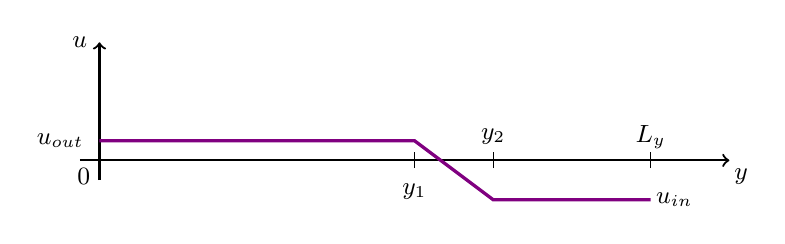
\begin{tikzpicture}
%\draw[fill=gray!23,gray!23](0,0) rectangle (10,3);
%\draw[step=0.5cm,gray,very thin] (0,0) grid (10,3); %background grid
\draw[thick,->] (0.75,1) -- (9,1)  ; 
\draw[thick,->] (1,0.75) -- (1,2.5)  ; 
\draw[-] (5,0.9) -- (5,1.1)  ; 
\draw[-] (6,0.9) -- (6,1.1)  ; 
\draw[-] (8,0.9) -- (8,1.1)  ; 
\draw[very thick, violet] (1,1.25)--(5,1.25) -- (6,0.5) -- (8,0.5) ; 
\node[] at (0.8,0.8) {\small $0$};
\node[] at (9.15,0.8) {\small $y$};
\node[] at (5,0.6) {\small $y_1$};
\node[] at (6,1.3) {\small $y_2$};
\node[] at (8,1.3) {\small $L_y$};
\node[] at (8.3,0.5) {\small $u_{in}$};
\node[] at (0.5,1.25) {\small $u_{out}$};
\node[] at (0.75,2.5) {\small $u$};
\end{tikzpicture}
\end{center}



The velocity on the side is given by
\begin{eqnarray}
u(y) &=& u_{out} \quad\quad y<y_1 \nn\\
u(y) &=& \frac{u_{in}-u_{out}}{y_2-y_1}(y-y_1) + u_{out} \quad\quad y_1<y<y_2 \nn\\
u(y) &=& u_{in} \quad\quad y>y_2 \nn
\end{eqnarray}
Note that $u_{in}$ and $u_{out}$ can be positive or negative, but 
of opposite signs.
The requirement for volume conservation is:
\[
\Phi=\int_{0}^{L_y} u(y) dy = 0
\]
Having chosen $u_{in}$ (the velocity of the plate), one can then compute $v_{out}$
as a function of $y_1$ and $y_2$.

\begin{eqnarray}
\Phi
&=&
\underbrace{\int_{0}^{y_1} u(y) dy}_{\Phi_1}  +
\underbrace{\int_{y_1}^{y_2} u(y) dy }_{\Phi_2}  +
\underbrace{\int_{y_2}^{L_y} u(y) dy }_{\Phi_3}\nn
\end{eqnarray}
with
\begin{eqnarray}
\Phi_1 &=& u_{out} y_1 \nn\\
\Phi_2 
&=& \int_{y_1}^{y_2} u(y) dy \nn\\
&=& \int_{y_1}^{y_2} \left[ \frac{u_{in}-u_{out}}{y_2-y_1}(y-y_1) + u_{out}   \right] dy \nn\\
&=& \int_{y_1}^{y_2} \frac{u_{in}-u_{out}}{y_2-y_1}(y-y_1)  dy  +   \int_{y_1}^{y_2}  u_{out} dy \nn\\
&=& \frac{u_{in}-u_{out}}{y_2-y_1} \int_{y_1}^{y_2} (y-y_1)  dy  +   (y_2-y_1) u_{out}  \nn\\
&=& \frac{u_{in}-u_{out}}{y_2-y_1} \left[ \frac12 y^2 - y_1y   \right]_{y_1}^{y_2} +   (y_2-y_1) u_{out}  \nn\\
&=& \frac{u_{in}-u_{out}}{y_2-y_1} ( \frac12 y_2^2 - y_1y_2 - \frac12y_1^2 + y_1^2 ) +   (y_2-y_1) u_{out}  \nn\\
&=& \frac{u_{in}-u_{out}}{y_2-y_1} \frac12 ( y_2^2 - 2y_1y_2 + y_1^2 ) +   (y_2-y_1) u_{out}  \nn\\
&=& \frac{u_{in}-u_{out}}{y_2-y_1} \frac12 ( y_2-y_1 )^2 +   (y_2-y_1) u_{out}  \nn\\
&=& (u_{in}-u_{out}) \frac12 ( y_2-y_1 ) +   (y_2-y_1) u_{out}  \nn\\
&=& \frac{1}{2}(u_{in}+u_{out})(y_2-y_1)  \nn\\
\Phi_3 &=& (L_y-y_2) u_{in} \nn
\end{eqnarray}
so that in the end
\begin{eqnarray}
\Phi &=& \Phi_1+\Phi_2+\Phi_3 \nn\\
&=& u_{out} [y_1 + \frac{1}{2}(y_2-y_1) ] + u_{in} [ \frac{1}{2}(y_2-y_1)  + (L_y-y_2) ] \nn\\
&=& u_{out}\frac{1}{2} (y_1 + y_2 ) + u_{in} [ L_y - \frac{1}{2}(y_1+y_2) ] \nn
\end{eqnarray}
and finally, solving for $u_{out}$
\begin{mdframed}[backgroundcolor=blue!5]
\[
u_{out} = -u_{in} \frac{ L_y - \frac{1}{2}(y_1+y_2)}{ \frac{1}{2} (y_1 + y_2 ) }
\]
\end{mdframed}


In some cases one may wish to prescribe a zero velocity 
below the 660 discontinuity (given by $y=y_1$) on the following 
figure:

\begin{center}
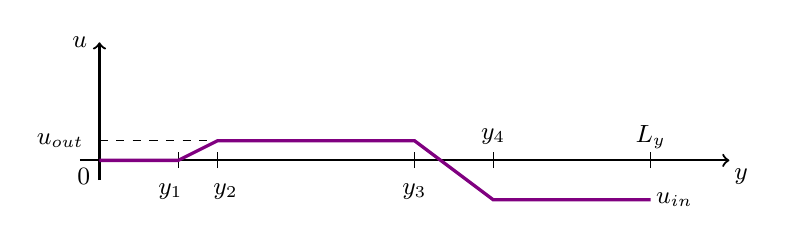
\begin{tikzpicture}
%\draw[fill=gray!23,gray!23](0,0) rectangle (10,3);
%\draw[step=0.5cm,gray,very thin] (0,0) grid (10,3); %background grid
\draw[thick,->] (0.75,1) -- (9,1)  ; 
\draw[thick,->] (1,0.75) -- (1,2.5)  ; 
\draw[-] (2,0.9) -- (2,1.1)  ; 
\draw[-] (2.5,0.9) -- (2.5,1.1)  ; 
\draw[-] (5,0.9) -- (5,1.1)  ; 
\draw[-] (6,0.9) -- (6,1.1)  ; 
\draw[-] (8,0.9) -- (8,1.1)  ; 
\draw[thin, dashed] (1,1.25) -- (2.5,1.25)  ; 
\draw[very thick, violet] (1,1)--(2,1)--(2.5,1.25)--(5,1.25) -- (6,0.5) -- (8,0.5) ; 
\node[] at (0.8,0.8) {\small $0$};
\node[] at (9.15,0.8) {\small $y$};
\node[] at (1.9,0.6) {\small $y_1$};
\node[] at (2.6,0.6) {\small $y_2$};
\node[] at (5,0.6) {\small $y_3$};
\node[] at (6,1.3) {\small $y_4$};
\node[] at (8,1.3) {\small $L_y$};
\node[] at (8.3,0.5) {\small $u_{in}$};
\node[] at (0.5,1.25) {\small $u_{out}$};
\node[] at (0.75,2.5) {\small $u$};
\end{tikzpicture}
\end{center}

 
\newpage %-----------------------------------------------------------------------------------------
\subsection{Periodic boundary conditions\label{ss_periodic}}\input{periodic} %---------------------
\newpage %-----------------------------------------------------------------------------------------
\subsection{Free-slip boundary conditions on annulus}\label{ss:fsbc_annulus}\begin{flushright} {\tiny {\color{gray} fsbc\_annulus.tex}} \end{flushright}
%~~~~~~~~~~~~~~~~~~~~~~~~~~~~~~~~~~~~~~~~~~~~~~~~~~~~~~~~~~~~~~~~~~~~~~~~~~~~~~~~~~~~~~~~~~~~~~~~~~

In the context of geodynamical modelling we often wish to prescribed free-slip 
boundary conditions on a given boundary of the domain. If the domain is a rectangle
which sides align with the Cartesian axis, then fixing $\upnu_x=0$ or $\upnu_y=0$
is simple and does indeed insure free-slip boundary conditions. 

However the situation is much more complicated in the case of a curved boundary, 
such as for instance the inner and outer boundaries of an annulus or spherical shell.

If the curved boundary is a circular, the procedure is as follows:
\begin{enumerate}
\item identify the node on the boundary which is to be fixed. 
\item compute its coordinate angle $\theta$ (and $\phi$ in 3D) 
\item do a rotation so as to bring it back onto the x-axis (2D) or z-axis (3D)
\item apply free slip boundary condition (now easy since parallel or perpendicular to axis)
\item rotate back
\end{enumerate}

This technique is implemented in \stone~\ref{f33}, \stone~\ref{f96} and \stone~\ref{f151}.

\paragraph{A few remarks about rotation matrices} 
In a given plane, the counter-clockwise rotation matrix by and angle $\theta$ is defined by 
\[
{\cal R}=
\left(
\begin{array}{cc}
\cos\theta & \sin\theta \\
-\sin\theta & \cos\theta
\end{array}
\right)
\]
The image of vector $\vec{V}$ by a rotation of angle $\theta$ is given by
\[
\vec{V}'={\cal R}\cdot \vec{V}
\]

Coordinate transformations of second-rank tensors involve the very same   
matrix as vector transforms. A transformation of the stress tensor ${\bm \sigma}$ ,
from the reference $xy$-coordinate system to ${\bm \sigma}'$ in a new $x'y'-$system is done as follows:
\[
{\bm \sigma}'={\cal R}\cdot {\bm \sigma}\cdot{\cal R}^T
\]



[from Wikipedia] A basic rotation (also called elemental rotation) is a rotation about one of the axes of a Coordinate system. 
The following three basic rotation matrices rotate vectors by an angle $\alpha$ 
about the x-, y-, or z-axis, in three dimensions, using the right-hand rule which codifies their 
alternating signs. 

\[
{\cal R}_x(\alpha)=
\left(
\begin{array}{ccc}
1 & 0 & 0 \\
0 & \cos\alpha & -\sin\alpha \\
0 & \sin\alpha & \cos\alpha
\end{array}
\right)
\]

\[
{\cal R}_y(\alpha)=
\left(
\begin{array}{ccc}
\cos\alpha & 0 & \sin\alpha \\
0 & 1 & 0 \\
-\sin\alpha & 0 &\cos\alpha
\end{array}
\right)
\]

\[
{\cal R}_z(\alpha)=
\left(
\begin{array}{ccc}
\cos\alpha & -\sin\alpha & 0\\
\sin\alpha & \cos\alpha & 0 \\
0 & 0 & 1 
\end{array}
\right)
\]

In my \elefant code
I first rotate around the $z$ axis by and angle $-\phi$ and then 
around axis $y$ by an angle $-\theta$ in the case of a spherical shell.

\[
{\cal R}_y(-\theta)=
\left(
\begin{array}{ccc}
\cos(-\theta) & 0 & \sin(-\theta) \\
0 & 1 & 0 \\
-\sin(-\theta) & 0 &\cos(-\theta)
\end{array}
\right)
=
\left(
\begin{array}{ccc}
\cos\theta & 0 & -\sin\theta \\
0 & 1 & 0 \\
\sin\theta & 0 &\cos\theta
\end{array}
\right)
\]

\[
{\cal R}_z(-\phi)
=
\left(
\begin{array}{ccc}
\cos(-\phi)& -\sin(-\phi) & 0\\
\sin(-\phi)& \cos(-\phi) & 0 \\
0 & 0 & 1 
\end{array}
\right)
=
\left(
\begin{array}{ccc}
\cos\phi& \sin\phi & 0\\
-\sin\phi& \cos\phi & 0 \\
0 & 0 & 1 
\end{array}
\right)
\]

These are the {\tt Rott} and {\tt Rotp} matrices in the routines.


\Literature
\begin{itemize}
\item 
Note that in some cases applying free slip boundary conditions on a curved boundary with a triangular mesh 
can be problematic as explained in \textcite{ditu13} (2013).
\item \fullcite{ensg82}
\item \fullcite{behr04} in which it is stated:\\
{\it 1. If the slip boundary coincides with a Cartesian coordinate plane, the implementation is trivial,
with the equations corresponding to the normal component of velocity simply being dropped
from the equation system.
2. If the slip boundary does not coincide with a Cartesian coordinate plane, the equations
corresponding to the velocity components at the boundary are locally aligned with the normal-
tangent-bi-tangent coordinate system, and the normal component of velocity is set to zero.
This procedure is described by \textcite{ensg82} (1982), who also advocate the use of consistent
normals for proper mass conservation.}
\end{itemize}
 %-

\newpage %%%%%%%%%%%%%%%%%%%%%%%%%%%%%%%%%%%%%%%%%%%%%%%%%%%%%%%%%%%%%%%%%%%%%%%%%%%%%%%%%%%%%%%%%%
\section{Open boundary conditions}\label{ss:openbc}\begin{flushright} {\tiny {\color{gray} openbc.tex}} \end{flushright}
%~~~~~~~~~~~~~~~~~~~~~~~~~~~~~~~~~~~~~~~~~~~~~~~~~~~~~~~~~~~~~~~~~~~~~~~~~~~~~~~~~~~~~~~~~~~~~~~~~~

So-called open boundary conditions have a special meaning in computational geodynamics. 
They usually refer to the boundary conditions on the sides of Cartesian models, 
usually looking at subduction or rifting processes. 

In the literature boundary conditions on the vertical sidewalls are usually 
\begin{itemize}
\item no-slip (no flow at the boundary), 
\item free slip (impermeable); 
\item open to some particular form of through-flow.
\end{itemize}

Free slip is the most commonly used boundary condition while prescribed in- and outflow 
or periodic boundary conditions are also common. (REF?)

Taken from \textcite{chgv12} (2012):
``Open boundaries for which the horizontal in- and outflow are defined by a fully 
internally developed flow, have hardly been used [...]. 
Such open boundaries basically prescribe a hydrostatic pressure condition on 
the boundary preventing the model to collapse while horizontal in and outflow is free, 
in the sense that it is driven by the internal dynamics and the usual condition of 
incompressible flow. 
Among the range of boundary conditions used, open boundaries may fit best to 
real-mantle flow conditions surrounding subduction zones.''

Two examples of the use of such boundary conditions were found in 
the literature: \textcite{qusp10} (2010) and \textcite{chgv12} (212).

We start again from the variational form of the momentum equation, and focus on the term containing 
the full stress tensor ${\bm \sigma}$. 
Let us look at the stress tensor gradient, multiplied by the basis function $\bN$, integrated over the domain:
\begin{eqnarray}
\int_V \bN {\vec \nabla}\cdot {\bm \sigma} \; dV 
&=&\int_V \left[ {\vec \nabla}\cdot(\bN {\bm \sigma}) -{\vec \nabla} \bN \cdot {\bm \sigma}\right] \; dV \nonumber\\
&=& \int_V  {\vec \nabla}\cdot(\bN {\bm \sigma})\;  dV -\int_V  {\vec \nabla}\bN \cdot {\bm \sigma} \; dV
\end{eqnarray}
The right term yields the $\K$ and $\G$ matrices after discretisation, as seen in Section~\ref{XXX}.
Turning to the left term, we then make use of the Green-Gauss divergence 
theorem\footnote{\url{https://en.wikipedia.org/wiki/Divergence_theorem}} which states that for 
a continuously differentiable vector field $\vec{F}$:
\[
\int_V ({\vec \nabla} \cdot {\vec F})\; dV = \int _S {\vec F}\cdot {\vec n} \; dS
\]
so that (applying it now to tensors):
\[
\int_V  {\vec \nabla}\cdot(\bN {\bm \sigma})\;  dV =\int_S  \bN {\bm \sigma} \cdot {\vec n} \;  dS
\]
This right hand side term is responsible for the surface 
boundary conditions and cannot be neglected if one 
wishes to implement stress boundary conditions, 
such as the so-called open boundary conditions. 

Note that in \textcite{lige17} (2017) the authors describe an iterative algorithm that 
allows them to control the actual force applied at the boundary by 
scaling the kinematical boundary conditions

%.................................................................
\subsection{Two-dimensional case - $Q_1 \times P_0$ elements}

On the following figure two elements are represented, one on the 
left boundary, one on the right boundary:
\begin{center}
\includegraphics[width=5cm]{images/openbc/drawing.png}
\end{center}

The prescribed traction on the leftt boundary is
\[
{\vec t}={\bm \sigma}\cdot {\vec n}=
\left(
\begin{array}{cc}
-p_{bc} & 0 \\
0 & -p_{bc}
\end{array}
\right)
\cdot
\left(
\begin{array}{c}
-1 \\ 0
\end{array}
\right)
=
\left(
\begin{array}{c}
p_{bc} \\ 0
\end{array}
\right)
\]
The integral on the side of the element is then 
\[
\int_\Gamma \bN_i {\vec t} \; dS
\]
for $i=1,2,3,4$, which yields the following elemental rhs vector:
\[
\vec{F}_{el}=
\int_{\Gamma_{14}} 
\left(
\begin{array}{c}
\bN_1(x,y) t_x(x,y)\\
\bN_1(x,y) t_y(x,y)\\
\bN_2(x,y) t_x(x,y)\\
\bN_2(x,y) t_y(x,y)\\
\bN_3(x,y) t_x(x,y)\\
\bN_3(x,y) t_y(x,y)\\
\bN_4(x,y) t_x(x,y)\\
\bN_4(x,y) t_y(x,y)
\end{array}
\right)
\; dS
\]
It is worth noting that the integral takes place on the edge $\Gamma_{14}$ 
so that $\bN_2$ and $\bN_3$ are identically zero on this edge
and also $t_y=0$ 
so 
\[
\vec{F}_{el}=
\left(
\begin{array}{c}
\int_{\Gamma_{14}}  \bN_1(x,y) t_x(x,y) dS\\
0 \\
0 \\ 0 \\ 0 \\ 0 \\
\int_{\Gamma_{14}} \bN_4(x,y) t_x(x,y) dS\\
0
\end{array}
\right)
\]
If the traction (applied pressure) is constant over the element, 
then  
\[
\vec{F}_{el}=
t_x
\left(
\begin{array}{c}
\int_{\Gamma_{14}}  \bN_1(x,y)  dS\\
0 \\
0 \\ 0 \\ 0 \\ 0 \\
\int_{\Gamma_{14}} \bN_4(x,y)  dS\\
0
\end{array}
\right)
=
t_x
\left(
\begin{array}{c}
\int_{y_1}^{y_4} \bN_1(x,y) dy\\
0 \\
0 \\ 0 \\ 0 \\ 0 \\
\int_{y_1}^{y_4} \bN_4(x,y) dy\\
0
\end{array}
\right)
=
\frac{t_x h_y}{2}
\left(
\begin{array}{c}
1 \\
0 \\
0 \\ 0 \\ 0 \\ 0 \\
1 \\
0
\end{array}
\right)
\]
where $h_y$ is the height of the element along the segment. 



On the right boundary, we have $\bN_2=0$ and $\bN_3=0$, and since $t_y=0$ then 
the corresponding additional elemental right hand side vector writes:
\[
\vec{F}_{el} =
-\frac{t_x h_y}{2}
\left(
\begin{array}{c}
0\\
0\\
1 \\
0\\
1 \\
0\\
0\\
0
\end{array}
\right)
\] 

In the case where the traction is not constant over the edge, a numerical quadrature rule 
must be employed to integrate $\int_\Gamma \bN_i t_x dS$.



%....................................................................
\subsection{Three-dimensional case - $Q_1 \times P_0$ elements}

The right hand side is $ndof \times ndim = 8\times 3 = 24$ long. 

\begin{center}
\includegraphics[width=5.5cm]{images/openbc/drawing3D.png}
\end{center}

\begin{itemize}
\item The face $r=-1$ is made of nodes 1,4,5,8, so $\vec{n}=(-1,0,0)$.
Since $t_y=0$ and $t_z=0$ and $\bN_2=\bN_3=\bN_6=\bN_7$ on this face:
{\tiny
\[
\vec{F}_{el}=
\int_{\Gamma_{1458}} 
\left(
\begin{array}{c}
\bN_1(x,y,z) t_x(x,y,z)\\
\bN_1(x,y,z) t_y(x,y,z)\\
\bN_1(x,y,z) t_z(x,y,z)\\
\bN_2(x,y,z) t_x(x,y,z)\\
\bN_2(x,y,z) t_y(x,y,z)\\
\bN_2(x,y,z) t_z(x,y,z)\\
\bN_3(x,y,z) t_x(x,y,z)\\
\bN_3(x,y,z) t_y(x,y,z)\\
\bN_3(x,y,z) t_z(x,y,z)\\
\bN_4(x,y,z) t_x(x,y,z)\\
\bN_4(x,y,z) t_y(x,y,z)\\
\bN_4(x,y,z) t_z(x,y,z)\\
\bN_5(x,y,z) t_x(x,y,z)\\
\bN_5(x,y,z) t_y(x,y,z)\\
\bN_5(x,y,z) t_z(x,y,z)\\
\bN_6(x,y,z) t_x(x,y,z)\\
\bN_6(x,y,z) t_y(x,y,z)\\
\bN_6(x,y,z) t_z(x,y,z)\\
\bN_7(x,y,z) t_x(x,y,z)\\
\bN_7(x,y,z) t_y(x,y,z)\\
\bN_7(x,y,z) t_z(x,y,z)\\
\bN_8(x,y,z) t_x(x,y,z)\\
\bN_8(x,y,z) t_y(x,y,z)\\
\bN_8(x,y,z) t_z(x,y,z)
\end{array}
\right)
\; dS
=
\int_{\Gamma_{1458}} 
\left(
\begin{array}{c}
\bN_1(x,y,z) t_x\\
0 \\
0 \\
0\\
0\\
0\\
0\\
0\\
0\\
\bN_4(x,y,z) t_x\\
0\\
0\\
\bN_5(x,y,z) t_x\\
0\\
0\\
0\\
0\\
0\\
0\\
0\\
0\\
\bN_8(x,y,z) t_x\\
0 \\
0
\end{array}
\right)
\; dS
=
t_x
\left(
\begin{array}{c}
\int_{\Gamma_{1458}} \bN_1(x,y,z) dS\\ 
0\\
0\\
0\\
0\\
0\\
0\\
0\\
0\\
\int_{\Gamma_{1458}} \bN_4(x,y,z) dS\\ 
0\\
0\\
\int_{\Gamma_{1458}} \bN_5(x,y,z) dS\\
0\\
0\\
0\\
0\\
0\\
0\\
0\\
0\\
\int_{\Gamma_{1458}}  \bN_8(x,y,z) dS\\
0\\
0
\end{array}
\right)
=
\frac{h_yh_y t_x}{4}
\left(
\begin{array}{c}
1 \\
0\\
0\\
0\\
0\\
0\\
0\\
0\\
0\\
1\\
0\\
0\\
1\\
0\\
0\\
0\\
0\\
0\\
0\\
0\\
0\\
1\\
0\\
0
\end{array}
\right)
\]
}


\item
The face $r=+1$ is made of nodes 2,3,6,7, so $\vec{n}=(1,0,0)$.
so the non-zero terms are in positions $(4,7,16,19)$.

\item
The face $s=-1$ is made of nodes 1,2,5,6, so $\vec{n}=(0,-1,0)$.
so the non-zero terms are in positions $(2,5,14,17)$.

\item
The face $s=+1$ is made of nodes 3,4,7,8, so $\vec{n}=(0,+1,0)$.
so the non-zero terms are in positions $(8,11,20,23)$.

\end{itemize}


%.................................................................
\subsection{Two-dimensional case - $Q_2 \times Q_1$ elements}

We here too assume that we wish to prescribe a traction on the sides of a 2D domain
which are aligned with the vertical axis.

\subsubsection{constant traction}

It is not fundamentally different, except that the element counts 9 nodes, 
so the vector is $9\times 2=18$ long. 
The internal numbering of the nodes is as follows:
\begin{verbatim}
 velocity    pressure
 3---6---2   3-------2
 |       |   |       |
 7   8   5   |       |
 |       |   |       |
 0---4---1   0-------1
\end{verbatim}

On the left boundary nodes 0,3,7 are involved while on the right 
boundary nodes 1,2,5 are.
Assuming once again $t_x$ constant over the edge and $t_y=0$, we
have on the left side:

\[
\vec{F}_{el}=
\int_{\Gamma_{073}} 
\left(
\begin{array}{c}
\bN_0(x,y) t_x(x,y)\\
\bN_0(x,y) t_y(x,y)\\
\bN_1(x,y) t_x(x,y)\\
\bN_1(x,y) t_y(x,y)\\
\bN_2(x,y) t_x(x,y)\\
\bN_2(x,y) t_y(x,y)\\
\bN_3(x,y) t_x(x,y)\\
\bN_3(x,y) t_y(x,y)\\
\bN_4(x,y) t_x(x,y)\\
\bN_4(x,y) t_y(x,y)\\
\bN_5(x,y) t_x(x,y)\\
\bN_5(x,y) t_y(x,y)\\
\bN_6(x,y) t_x(x,y)\\
\bN_6(x,y) t_y(x,y)\\
\bN_7(x,y) t_x(x,y)\\
\bN_7(x,y) t_y(x,y)\\
\bN_8(x,y) t_x(x,y)\\
\bN_8(x,y) t_y(x,y)
\end{array}
\right)
dS
=
t_x 
\left(
\begin{array}{c}
\int_{\Gamma_{073}} \bN_0(x,y) dS\\
0 \\ 0 \\ 0 \\ 0 \\ 0 \\
\int_{\Gamma_{073}} \bN_3(x,y) dS \\
0 \\ 0 \\ 0 \\ 0 \\ 0 \\ 0 \\ 0 \\
\int_{\Gamma_{073}}  \bN_7(x,y) dS \\
0 \\ 0 \\ 0
\end{array}
\right)
=
t_x  \frac{h_y}{2}
\left(
\begin{array}{c}
\int_{-1}^{+1} \bN_0(r=-1,s) ds\\
0 \\ 0 \\ 0 \\ 0 \\ 0 \\
\int_{-1}^{+1} \bN_3(r=-1,s) ds \\
0 \\ 0 \\ 0 \\ 0 \\ 0 \\ 0 \\ 0 \\
\int_{-1}^{+1}  \bN_7(r=-1,s) ds \\
0 \\ 0 \\ 0
\end{array}
\right)
\]
We then compute
\begin{eqnarray}
\int_{-1}^{+1} \bN_0(r=-1,s) ds 
&=& \int_{-1}^{+1} \frac{1}{2}s(s-1) ds = \frac{1}{3} \\
\int_{-1}^{+1} \bN_3(r=-1,s) ds 
&=& \int_{-1}^{+1} \frac{1}{2}s(s+1) ds = \frac{1}{3} \\
\int_{-1}^{+1} \bN_7(r=-1,s) ds 
&=& \int_{-1}^{+1} (1-s^2) ds = \frac{4}{3} 
\end{eqnarray}
Note that the sum of the three terms is 2, as expected: on the edge
we have $\bN_0+\bN_3+\bN_7 =1$ so that the integral of the sum over the 
interval [-1,1] yields 2. Finally 
\[
\vec{F}_{el}
=
\frac{t_x  h_y}{6}
\left(
\begin{array}{c}
1 \\
0 \\
0 \\
0 \\
0 \\
0 \\
1 \\
0 \\
0 \\
0 \\
0 \\
0 \\
0 \\
0 \\
4 \\
0 \\
0 \\
0
\end{array}
\right)
\]
This is implemented in \stone 61, 64, 146, 148.





On the right boundary, we need to compute (careful with sign when implementing!)
\[
\vec{F}_{el}=
\int_{\Gamma_{152}} 
\left(
\begin{array}{c}
\bN_0(x,y) t_x(x,y)\\
\bN_0(x,y) t_y(x,y)\\
\bN_1(x,y) t_x(x,y)\\
\bN_1(x,y) t_y(x,y)\\
\bN_2(x,y) t_x(x,y)\\
\bN_2(x,y) t_y(x,y)\\
\bN_3(x,y) t_x(x,y)\\
\bN_3(x,y) t_y(x,y)\\
\bN_4(x,y) t_x(x,y)\\
\bN_4(x,y) t_y(x,y)\\
\bN_5(x,y) t_x(x,y)\\
\bN_5(x,y) t_y(x,y)\\
\bN_6(x,y) t_x(x,y)\\
\bN_6(x,y) t_y(x,y)\\
\bN_7(x,y) t_x(x,y)\\
\bN_7(x,y) t_y(x,y)\\
\bN_8(x,y) t_x(x,y)\\
\bN_8(x,y) t_y(x,y)
\end{array}
\right)
dS
=
t_x 
\left(
\begin{array}{c}
0 \\ 0 \\
\int_{\Gamma_{125}} \bN_1(x,y) dS \\ 0 \\ 
\int_{\Gamma_{125}} \bN_2(x,y) dS \\ 0 \\
0 \\ 0 \\
0 \\ 0 \\ 
\int_{\Gamma_{125}} \bN_5(x,y) dS \\
0 \\ 0 \\ 
0 \\ 0 \\ 
0 \\ 0
\end{array}
\right)
=
t_x  \frac{h_y}{2}
\left(
\begin{array}{c}
0 \\ 0 \\
\int_{-1}^{+1} \bN_1(-1,s) ds \\ 0 \\ 
\int_{-1}^{+1} \bN_2(-1,s) ds \\ 0 \\
0 \\ 0 \\
0 \\ 0 \\
\int_{-1}^{+1} \bN_5(-1,s) ds \\
0 \\ 0 \\
0 \\ 0 \\
0 \\ 0 
\end{array}
\right)
=
\frac{t_x h_y}{6}
\left(
\begin{array}{c}
0 \\ 0 \\
1 \\ 0 \\
1 \\ 0 \\
0 \\ 0 \\
0 \\ 0 \\
4 \\ 0 \\
0 \\ 0 \\
0 \\ 0 \\
0 \\ 0
\end{array}
\right)
\]

%---------------------------------------------------------------
\subsubsection{linear traction}

Let us now turn to the case where the traction we wish to apply 
on the boundary is not piecewise constant but linear.
We set $t_x(y)=ay+b$, so that on the right side (nodes, 1,2,5), we have to compute

\begin{eqnarray}
\int_{\Gamma_{125}} \bN_1(x,y) t_x(y) dS 
&=&\int_{\Gamma_{125}} \bN_1(x,y) (ay+b) dy \nn\\
&=&\frac{h_y}{2} \int_{-1}^1 \bN_1(r=1,s) [ay(s)+b] ds \nn
\end{eqnarray}
We have 
\[
s(y)=\frac{2}{h_y}(y-y_1)-1 
\qquad
\text{or}
\qquad
y(s)= \frac{h_y}{2}(s+1) +y_1
\]
and
\[
\bN_1(r,s) 
= \frac{1}{2}r(r+1)\frac{1}{2}s(s-1)
\qquad
\Rightarrow
\qquad
\bN_1(r=1,s) 
= \frac{1}{2}1(1+1)\frac{1}{2}s(s-1) 
= \frac{1}{2}s(s-1) 
\]
Then
\begin{eqnarray}
\int_{\Gamma_{125}} \bN_1(x,y) t_x(y) dS 
&=&\frac{h_y}{2} \int_{-1}^1 \bN_1(r=1,s) \left[ a \left(\frac{h_y}{2}(s+1) +y_1\right) +b \right] ds \nn\\
&=&\frac{h_y}{2} \int_{-1}^1 \frac12 s(s-1) \left[ a \left(\frac{h_y}{2}(s+1) +y_1\right) +b \right] ds \nn\\
&=&\frac{h_y}{4} \int_{-1}^1 s(s-1) \left[ \frac{a h_y}{2}(s+1) + (ay_1+b) \right] ds \nn\\
&=& \frac{h_y}{4} \left[
\frac{a h_y}{2} \int_{-1}^1 s(s-1) (s+1)  ds 
+(ay_1+b) \int_{-1}^1 s(s-1)   ds 
\right] \nn\\
&=& \frac{h_y}{4} 
\frac{a h_y}{2} \underbrace{\int_{-1}^1 s(s^2-1)  ds}_{=0} 
+\frac{h_y}{4} (ay_1+b) \underbrace{\int_{-1}^1 s(s-1)   ds}_{=2/3} \nn\\
&=& \frac{h_y}{6} (ay_1+b)
\end{eqnarray}

Let us now turn to $\bN_2$:
\[
\bN_2(r,s) = \frac12 r(r+1) \frac12 s(s+1)
\qquad
\Rightarrow
\qquad
\bN_2(r=1,s) = \frac12 s(s+1)
\]
Then
\begin{eqnarray}
\int_{\Gamma_{125}} \bN_2(x,y) t_x(y) dS 
&=&\frac{h_y}{2} \int_{-1}^1 \bN_2(r=1,s) \left[ a \left(\frac{h_y}{2}(s+1) +y_1\right) +b \right] ds \nn\\
&=&\frac{h_y}{2} \int_{-1}^1 \frac12 s(s+1) \left[ a \left(\frac{h_y}{2}(s+1) +y_1\right) +b \right] ds \nn\\
&=&\frac{h_y}{4} \int_{-1}^1 s(s+1) \left[ \frac{a h_y}{2}(s+1) + (ay_1+b) \right] ds \nn\\
&=& \frac{h_y}{4} \left[
\frac{a h_y}{2} \int_{-1}^1 s(s+1) (s+1)  ds 
+(ay_1+b) \int_{-1}^1 s(s+1)   ds 
\right] \nn\\
&=& \frac{h_y}{4} 
\frac{a h_y}{2} \underbrace{\int_{-1}^1 s(s+1)^2  ds}_{=4/3} 
+\frac{h_y}{4} (ay_1+b) \underbrace{\int_{-1}^1 s(s+1)  ds}_{=2/3} \nn \\
&=& \frac{h_y}{6} \left( a h_y + ay_1+b   \right)
\end{eqnarray}



And finally let us turn to $\bN_5$:
\[
\bN_5(r,s) = \frac12 r(r+1) (1-s^2)
\qquad
\Rightarrow
\qquad
\bN_5(r=1,s) =  (1-s^2)
\]
then
\begin{eqnarray}
\int_{\Gamma_{125}} \bN_5(x,y) t_x(y) dS 
&=&\frac{h_y}{2} \int_{-1}^1 \bN_2(r=1,s) \left[ a \left(\frac{h_y}{2}(s+1) +y_1\right) +b \right] ds \nn\\
&=&\frac{h_y}{2} \int_{-1}^1  (1-s^2) \left[ a \left(\frac{h_y}{2}(s+1) +y_1\right) +b \right] ds \nn\\
&=&\frac{h_y}{2} \int_{-1}^1 (1-s^2) \left[ \frac{a h_y}{2}(s+1) + (ay_1+b) \right] ds \nn\\
&=& \frac{h_y}{2} \left[
\frac{a h_y}{2} \int_{-1}^1 (1-s^2) (s+1)  ds 
+(ay_1+b) \int_{-1}^1 (1-s^2)   ds 
\right] \nn\\
&=& \frac{h_y}{2} \frac{a h_y}{2} \underbrace{\int_{-1}^1 (1-s^2)(1+s)  ds}_{=4/3} 
+\frac{h_y}{2} (ay_1+b) \underbrace{\int_{-1}^1 (1-s^2)  ds}_{=4/3} \nn \\
&=& \frac{h_y}{6} \left( 2 a h_y + 4ay_1+4 b   \right)
\end{eqnarray}
Note that by setting $a=0$ and $b=t_x$ we recover the expressions above for a 
piecewise constant value.

If we know $p_1$ and $p_2$ (say, for example that the lithostatic pressure has been computed on these nodes
and we wish to prescribe it on the side) then 
\[
t_y=ay+b = \underbrace{\frac{p_2-p_1}{y_2-y_1}}_{=a} y + \underbrace{p_1-\frac{p_2-p_1}{y_2-y_1} y_1}_{=b}
\]

On the left side (nodes 0,7,3), we have to compute
\begin{eqnarray}
\int_{073} \bN_0(x,y) (ay+b) dS
&=& \frac{h_y}{2} \int_{-1}^{+1} \bN_0(r=-1,s) [ay(s)+b] ds \\
\int_{073} \bN_3(x,y) (ay+b) dS 
&=& \frac{h_y}{2} \int_{-1}^{+1} \bN_3(r=-1,s) [ay(s)+b] ds  \\
\int_{073} \bN_7(x,y) (ay+b) dS 
&=& \frac{h_y}{2} \int_{-1}^{+1} \bN_7(r=-1,s) [ay(s)+b] ds  
\end{eqnarray}
with 
\begin{align}
\bN_0 (r,s) &= \frac12 r(r-1) \frac12 s(s-1)  \rightarrow  \bN_0 (-1,s) &=  \frac12 s(s-1) \nonumber\\  
\bN_3 (r,s) &= \frac12 r(r-1) \frac12 (1-s^2) \rightarrow  \bN_3 (-1,s) &=  (1-s^2) \nonumber\\
\bN_7 (r,s) &= \frac12 r(r-1) \frac12 s(s+1)  \rightarrow  \bN_7 (-1,s) &=  \frac12 s(s+1) \nonumber
\end{align}


If we know $p_0$ and $p_3$ then 
\[
t_x=ay+b = \underbrace{\frac{p_3-p_0}{y_3-y_0}}{=a} y + \underbrace{p_0-\frac{p_3-p_0}{y_3-y_0} y_0}_{=b}
\]










%\begin{center}
%\includegraphics[width=4cm]{FEM/openbc/openbc1.png}
%\includegraphics[width=4cm]{FEM/openbc/openbc2.png}\\
%{\small Example of a Stokes sphere sinking when 
%both $y=0$ and $y=L_y$ walls are subjected to
%open boundary conditions.}
%\end{center}


%.................................................................
\subsection{Two-dimensional case - Linear triangle elements}

Let us assume we want to apply a stress on the face 13 of the following element:
\begin{verbatim}
   1-------------3
    \           /
     \         /
      \       /
       \     /
        \   /
         \ /
          2
\end{verbatim}

The integral on the side of the element is $\int_\Gamma \bN_i {\vec t} \; dS$
for $i=1,2,3$, which yields the following elemental rhs vector:
\[
\vec{F}_{el}=
\int_{\Gamma_{13}} 
\left(
\begin{array}{c}
\bN_1(x,y) t_x(x,y)\\
\bN_1(x,y) t_y(x,y)\\
\bN_2(x,y) t_x(x,y)\\
\bN_2(x,y) t_y(x,y)\\
\bN_3(x,y) t_x(x,y)\\
\bN_3(x,y) t_y(x,y)
\end{array}
\right)
\; dS
=
\int_{\Gamma_{13}} 
\left(
\begin{array}{c}
0\\
\bN_1(x,y) t_y(x,y)\\
0\\
0\\
0\\
\bN_3(x,y) t_y(x,y)
\end{array}
\right)
\; dS
\]
since $t_x=0$ and there function $\bN_2$ will be zero on the edge.

We also arbitrarily set $y_1=y_3=0$. We have seen in Section~\ref{shpfct2d} that 
the basis functions (expressed as a function of the real coordinates $x,y$) 
for a linear triangle are given by:
\begin{eqnarray}
\bN_1(x,y) &=& \frac{1}{D}[(x_2y_3-x_3y_2) + (y_2-y_3)x + (x_3-x_2)y] \nn\\
\bN_2(x,y) &=& \frac{1}{D}[(x_3y_1-x_1y_3) + (y_3-y_1)x + (x_1-x_3)y] \nn\\
\bN_3(x,y) &=& \frac{1}{D}[(x_1y_2-x_2y_1) + (y_1-y_2)x + (x_2-x_1)y] \nn
\end{eqnarray}
with 
\[
D = 
\left|
\begin{array}{ccc}
1 & x_1 & y_1 \\
1 & x_2 & y_2 \\
1 & x_3 & y_3 
\end{array}
\right|
=
\left|
\begin{array}{ccc}
1 & x_1 & 0 \\
1 & x_2 & y_2 \\
1 & x_3 & 0 
\end{array}
\right|
=
-x_3y_2+x_1y_2
= y_2(x_1-x_3)
\]


\begin{eqnarray}
\int_{x_1}^{x_3} \bN_1(x,y=0) dx 
&=& \frac{1}{D} \int_{x_1}^{x_3} [(x_2y_3-x_3y_2) + (y_2-y_3)x ] \nn\\
&=& \frac{1}{D} \int_{x_1}^{x_3} [-x_3y_2 + y_2 x ] \qquad \text{since} y_1=y_3=0 \nn\\
&=& \frac{y_2}{D} \int_{x_1}^{x_3} (-x_3 +  x ) dx \nn\\
&=& \frac{y_2}{y_2(x_1-x_3)  } [ -x_3 x + \frac{1}{2}x^2]_{x_1}^{x_3} \nn\\ 
&=& \frac{1}{x_1-x_3 } [ -x_3 (x_3-x_1) + \frac{1}{2}(x_3^2-x_1^2)] \nn\\
&=& \frac{1}{x_1-x_3 } [ x_3 (x_1-x_3) + \frac{1}{2}(x_3-x_1)(x_3+x_1)] \nn\\
&=&  x_3 - \frac{1}{2}(x_3+x_1) \nn\\
&=&  \frac{1}{2} (x_3-x_1) \\
\int_{x_1}^{x_3} \bN_3(x,y=0) dx
&=& \frac{1}{D} \int_{x_1}^{x_3}    [(x_1y_2-x_2y_1) + (y_1-y_2)x ] dx \nn\\
&=& \frac{1}{D} \int_{x_1}^{x_3}    [x_1y_2 - y_2x ] dx \nn\\
&=& \frac{y_2}{D} \int_{x_1}^{x_3}    [x_1 - x ] dx \nn\\
&=& \frac{y_2}{y_2(x_1-x_3) } [x_1 x - \frac{1}{2} x^2]_{x_1}^{x_3}  \nn\\
&=& \frac{1}{x_1-x_3} [x_1 (x_3-x_1) - \frac{1}{2} (x_3^2-x_1^2)] \nn\\
&=& -x_1  + \frac{1}{2} (x_3+ x_1) \nn\\
&=& \frac{1}{2}( x_3 -x_1 )
\end{eqnarray}
Finally
\[
\vec{F}_{el}=
\frac{h t_y}{2}
\left(
\begin{array}{c}
0\\
1 \\
0\\
0\\
0\\
1 
\end{array}
\right)
\]





 %--------------------------------

\newpage %%%%%%%%%%%%%%%%%%%%%%%%%%%%%%%%%%%%%%%%%%%%%%%%%%%%%%%%%%%%%%%%%%%%%%%%%%%%%%%%%%%%%%%%%%
\section{About nullspaces} 
\subsection{Pressure normalisation, nullspace\label{ss_pnorm}} \begin{flushright} {\tiny {\color{gray} pressure\_normlisation.tex}} \end{flushright}
%~~~~~~~~~~~~~~~~~~~~~~~~~~~~~~~~~~~~~~~~~~~~~~~~~~~~~~~~~~~~~~~~~~~~~~~~~~~~~~~~~~~~~~~~~~~~~~~~~~


%..................................................
\subsubsection{Basic idea and naive implementation}

When Dirichlet boundary conditions are imposed everywhere on the boundary, 
pressure is only present by its gradient in 
the equations. It is thus determined up to an arbitrary constant (one speaks then 
of a nullspace of size 1).  \index{general}{Nullspace}
In such a case, one commonly impose the average of the pressure over the whole domain or on 
a subset of the boundary 
to have a zero average, i.e.
\begin{equation}
\int_\Omega p\; dV = 0
\end{equation}

Let us assume for example/simplicity that we are using \QonePzero elements. The pressure is constant 
inside each element so the integral above becomes:
\begin{equation}
\int_\Omega p\; dV = 
\sum_e  \int_{\Omega_e} p\; dV = 
\sum_e  p_e \int_{\Omega_e}\; dV = 
\sum_e  p_e V_e = 0
\end{equation}
where the sum runs over all elements $e$ of volume $V_e$.
This can be rewritten 
\[
\vec{L} \cdot \vec{\cal P}=0
\] 
and it is a constraint on the pressure solution which couples {\it all} pressure dofs. 
We can associate to it a Lagrange multiplier $\lambda$ so that we must solve the modified Stokes system:
\[
\left(
\begin{array}{ccc}
\K & \G & 0\\ 
\G^T & 0 & \vec{L}^T \\
0 & \vec{L} & 0
\end{array}
\right)
\cdot
\left(
\begin{array}{c}
\vec{\cal V} \\ \vec{\cal P} \\ \lambda
\end{array}
\right)
=
\left(
\begin{array}{c}
\vec{f} \\ \vec{h} \\ 0
\end{array}
\right)
\]
When higher order spaces are used for pressure (continuous or discontinuous)
one must then carry out the above integration numerically by means of (usually)
a Gauss-Legendre quadrature.

Although valid, this approach has one main disadvantage: it makes the Stokes matrix larger (although
marginally so -- only one row and column are added), but more importantly it prevents the use of some
of the solving strategies of Section \ref{sec:solvers}.


%..................................................
\subsubsection{Implementation -- the real deal}

Here is what Bochev and Gunzburger \cite[Section 7.6.4]{bogu09} have to say about this:
"[...] practical implementations cheat by substituting enforcement of the true zero mean constraint by using
procedures collectively known as setting the pressure datum. These procedures essentially 
amount to removing one degree of freedom from the pressure space.
Setting the pressure datum can be accomplished in many different ways, ranging
from specifying a pressure value at a grid node to more complicated approaches in
which a boundary traction is specified at a single node in lieu of the velocity condition; 
see [16, 24, 191] and the references cited therein for more details. Not surprisingly, 
in practice, the simplest approach of fixing the pressure value at a node also
happens to be the most widely used in practice."




The idea is actually quite simple and requires two steps:
\begin{enumerate}
\item remove the null space by prescribing the pressure at one location and solve the system;
\item post-process the pressure so as to arrive at a pressure field which fulfils the required normalisation (surface, volume, ...)
\end{enumerate}

The reason why it works is as follows: a constant pressure value lies in the null space, so that one can 
add or delete any value to the pressure field without consequence. As such I can choose said constant such that 
the pressure at a given node/element is zero. All other computed pressures are then relative to that one. 
The post-processing step will redistribute a constant value to all pressures (it will shift them up or down)
so that the normalising condition is respected. 


\Literature

In \url{https://scicomp.stackexchange.com/questions/27645/pressure-boundary-condition-in-lid-driven-cavity-using-finite-element-method}
we find:
{\it 
Zero mean pressure space is used for convenience when one is interested in FEA theory (basically, we cannot 
enforce $p(x_0)=p_0$ for $p \in L^2$ since it does not make sense); from the computational point of view, 
it is easier to fix one of the pressure DOFs (although you can subtract mean value at the post–processing step 
if you want to). When you are working w/ polynomial spaces—and this is exactly what you do in FEM 
-it is perfectly fine to enforce $p(x_0)=p_0$. Handle this constraint like you usually handle Dirichlet 
BCs (e.g., via modifying your matrix). It is also fine to ignore this constraint in some 
cases (e.g., Krylov solvers can do fine with this).
}


\url{
https://scicomp.stackexchange.com/questions/25134/mixed-finite-element-method-for-the-stokes-system-some-implementation-details}





 %----
\subsection{Removing rotational nullspace\label{ss_nullspace}} \input{nullspace} %-----------------

